\documentclass[12pt]{article}

% Combined LaTeX file for arXiv submission

% Cleaned preamble for CMP submission.
% This file intentionally avoids aggressive layout changes or warning suppression.

% Keep layout changes minimal for journal production.
% If CMP requests explicit page geometry, re-enable the geometry package.
%\usepackage[a4paper, margin=2.5cm]{geometry}

\usepackage{amsmath,amssymb,amsthm}
\usepackage{mathtools}
\usepackage[T1]{fontenc}
\usepackage{hyperref}
\usepackage{cleveref}
\usepackage{tikz}
\usetikzlibrary{positioning}
\usepackage{booktabs}
\usepackage{enumitem}
\usepackage[hypcap=false]{caption}
\usepackage[expansion=false,protrusion=true,verbose=silent]{microtype}
\usepackage{lineno}
\usepackage{cite}

% Review mode (off for submission by default)
\newif\ifdraft
\draftfalse
\ifdraft
  \usepackage{setspace}
  \doublespacing
  \linenumbers
\fi

\hypersetup{
  hidelinks,
  pdftitle={The Angular Momentum Penrose Inequality},
  pdfauthor={Da Xu},
  pdfkeywords={Penrose inequality, angular momentum, Kerr spacetime, MOTS, Jang equation}
}

% Theorem environments
\theoremstyle{plain}
\newtheorem{theorem}{Theorem}[section]
\newtheorem{conjecture}[theorem]{Conjecture}
\newtheorem{proposition}[theorem]{Proposition}
\newtheorem{lemma}[theorem]{Lemma}
\newtheorem{corollary}[theorem]{Corollary}

\theoremstyle{definition}
\newtheorem{definition}[theorem]{Definition}
\newtheorem{example}[theorem]{Example}

\theoremstyle{remark}
\newtheorem{remark}[theorem]{Remark}

% Custom commands
\newcommand{\ADM}{\mathrm{ADM}}
\newcommand{\R}{\mathbb{R}}
\newcommand{\MOTS}{\mathrm{MOTS}}
\newcommand{\DEC}{\mathrm{DEC}}
\newcommand{\tr}{\mathrm{tr}}
\newcommand{\Ric}{\mathrm{Ric}}
\newcommand{\Rm}{\mathrm{Rm}}
\newcommand{\Div}{\mathrm{div}}
\DeclareMathOperator{\ind}{ind}
\DeclareMathOperator{\coker}{coker}
\newcommand{\tM}{\tilde{M}}
\newcommand{\tg}{\tilde{g}}
\newcommand{\bg}{\bar{g}}
\newcommand{\bM}{\bar{M}}
\newcommand{\momdens}{\boldsymbol{j}}

% Notation clarification:
%   - \Hoelder (\beta) for the H\"older exponent in C^{k,\beta} spaces
%   - \Komarform (\alpha_J) for the Komar 1-form encoding angular momentum
\newcommand{\Hoelder}{\beta}
\newcommand{\Komarform}{\alpha_J}

% Allow page breaks in equations
\allowdisplaybreaks

% Mild help for line breaking
\emergencystretch=1em
\tolerance=2000

\setcounter{tocdepth}{2}
\raggedbottom

\begin{document}


% --- Start of title-abstract.tex ---
% Title, Abstract, and Table of Contents
% This file should be included after \begin{document}
% Formatted for Communications in Mathematical Physics submission

\begin{center}
{\LARGE\bfseries The Angular Momentum Penrose Inequality}

\vspace{0.3cm}

{\large A Proof via the Extended Jang--Conformal--AMO Method}

\vspace{1cm}

{\large Da Xu}

\vspace{0.3cm}

{\itshape China Mobile Research Institute\\
Beijing 100053, China\\
E-mail: xuda@chinamobile.com}

\vspace{0.3cm}

\end{center}

\vspace{1cm}
\begin{abstract}
We prove the Angular Momentum Penrose Inequality: for asymptotically flat, axisymmetric initial data $(M^3, g, K)$ satisfying the dominant energy condition with vacuum in the exterior region, and containing an outermost strictly stable marginally outer trapped surface (MOTS) $\Sigma$ of area $A$ and Komar angular momentum $J$,
\[
M_{\ADM} \geq \sqrt{\frac{A}{16\pi} + \frac{4\pi J^2}{A}},
\]
with equality if and only if the data arises from a slice of the Kerr spacetime.

The proof introduces a four-stage Jang--conformal--AMO method: (1)~solve an axisymmetric Jang equation with twist as a lower-order perturbation; (2)~solve an angular-momentum-modified Lichnerowicz equation; (3)~establish angular momentum conservation via Stokes' theorem for closed 2-forms; (4)~apply the Dain--Reiris sub-extremality bound. The key innovation is the AM-Hawking mass $m_{H,J}(t) := \sqrt{m_H^2(t) + 4\pi J^2/A(t)}$, which is monotonically non-decreasing along the $p$-harmonic flow and converges to $M_{\ADM}$.

As a methodological application, we outline a new proof strategy for the Charged Penrose Inequality $M_{\ADM} \geq M_{\mathrm{irr}} + Q^2/(4M_{\mathrm{irr}})$ for non-rotating Einstein--Maxwell data, demonstrating the versatility of the Jang--conformal--AMO framework. This charged case is presented as a proof outline; complete rigorous proofs exist in the literature \cite{mars2009, khuri2015charged}.
\end{abstract}

\vspace{0.5cm}
\noindent\textbf{Keywords:} Penrose inequality, angular momentum, Kerr spacetime, marginally outer trapped surfaces, Jang equation, conformal method, positive mass theorem

\vspace{0.3cm}
\noindent\textbf{Mathematics Subject Classification (2020):} 83C57, 53C21, 35J60, 83C40

\tableofcontents

% --- End of title-abstract.tex ---

% --- Start of sec01-introduction.tex ---
\section{Introduction}
%=============================================================================

\subsection{Historical Context and Physical Motivation}

The Penrose inequality, conjectured by Roger Penrose in 1973 \cite{penrose1973}, encapsulates a fundamental principle of black hole physics: \textbf{black holes cannot be ``underweight'' for their size}. It relates the ADM mass of an asymptotically flat spacetime to the area of its black hole horizons:
\begin{equation}\label{eq:penrose}
    M_{\ADM} \geq \sqrt{\frac{A}{16\pi}},
\end{equation}
where $A$ is the area of the outermost marginally outer trapped surface (MOTS). This inequality was established for time-symmetric (Riemannian) initial data by Huisken--Ilmanen \cite{huisken2001} using inverse mean curvature flow and by Bray \cite{bray2001} using conformal flow. The spacetime (non-time-symmetric) case has been studied extensively using the Jang equation approach \cite{braykhuri2010, hankhuri2013}.

However, the classical formulation \eqref{eq:penrose} does not account for the \textbf{angular momentum} of the black hole. For rotating (Kerr) black holes, angular momentum directly affects the horizon structure and is a conserved quantity under Einstein evolution.

\begin{definition}[Sub-Extremality]\label{def:sub-extremal}
A Kerr black hole with mass $M$ and angular momentum $J = aM$ is called \textbf{sub-extremal} if $|a| < M$, \textbf{extremal} if $|a| = M$, and \textbf{super-extremal} (or naked singularity) if $|a| > M$. Equivalently, in terms of the dimensionless spin $\chi := a/M = J/M^2$: sub-extremal means $|\chi| < 1$. For an axisymmetric MOTS with area $A$ and Komar angular momentum $J$, the \textbf{sub-extremality condition} is $A \geq 8\pi|J|$, which is equivalent to the existence of a Kerr solution with matching $(A, J)$. The \textbf{sub-extremality factor} appearing in monotonicity formulas is:
\[
1 - \frac{64\pi^2 J^2}{A^2} = 1 - \left(\frac{8\pi|J|}{A}\right)^2.
\]
\textbf{Key algebraic fact:} This factor is non-negative \textbf{if and only if} $A \geq 8\pi|J|$. Indeed, $1 - (8\pi|J|/A)^2 \geq 0$ is equivalent to $(8\pi|J|/A)^2 \leq 1$, i.e., $8\pi|J| \leq A$. At the extremal limit ($A = 8\pi|J|$), the factor vanishes; for sub-extremal configurations ($A > 8\pi|J|$), it is strictly positive. The Dain--Reiris inequality \cite{dain2011} ensures this factor is non-negative for all stable MOTS in axisymmetric data satisfying DEC.
\end{definition}

The Kerr solution with mass $M$ and angular momentum $J = aM$ (where $a$ is the spin parameter with $|a| \leq M$ for sub-extremal black holes; see Definition~\ref{def:sub-extremal}) has horizon area
\[
A_{\text{Kerr}} = 8\pi M(M + \sqrt{M^2 - a^2}),
\]
which depends nontrivially on the spin parameter $a$. This motivates the search for a generalized Penrose inequality that incorporates both horizon area and angular momentum.

\subsection{Main Result}

We prove the natural extension incorporating angular momentum:

\begin{theorem}[Angular Momentum Penrose Inequality]\label{thm:main}
Let $(M^3, g, K)$ be an asymptotically flat initial data set satisfying:
\begin{enumerate}[label=\textup{(H\arabic*)}]
    \item \textbf{Dominant energy condition:} $\mu \geq |\momdens|_g$, where 
    \[
    \mu = \frac{1}{2}(R_g + (\tr_g K)^2 - |K|_g^2)
    \]
    is the energy density and $\momdens$ is the momentum density vector field (see Remark~\ref{rem:notation});
    \item \textbf{Axisymmetry:} There exists a Killing field $\eta = \partial_\phi$ generating rotations, with $\eta \neq 0$ on $M \setminus \Gamma$ where $\Gamma$ denotes the rotation axis;\footnotemark[1]
    \item \textbf{Vacuum in exterior region:} The constraint equations hold with $\mu = |\momdens| = 0$ in the \textbf{exterior region} $M_{\mathrm{ext}} := M \setminus \overline{\mathrm{Int}(\Sigma)}$, where $\mathrm{Int}(\Sigma)$ denotes the bounded component of $M \setminus \Sigma$. This hypothesis is \textbf{essential} for angular momentum conservation along the flow (see Remark~\ref{rem:vacuum-critical});
    \item \textbf{Strictly stable outermost MOTS:} There exists an outermost MOTS $\Sigma \subset M$ that is \textbf{strictly stable}, i.e., the principal eigenvalue of the MOTS stability operator (Definition~\ref{def:MOTS}) satisfies $\lambda_1(L_\Sigma) > 0$.
\end{enumerate}
Let $A := \int_\Sigma dA_g$ denote the area of $\Sigma$ \textbf{with respect to the physical metric $g$}. Let $\nu$ denote the \textbf{outward-pointing} unit normal to $\Sigma$ (i.e., pointing toward spatial infinity, satisfying $\langle \nu, \nabla r \rangle > 0$ asymptotically for any radial coordinate $r$). Define the Komar angular momentum:
\[
J := \frac{1}{8\pi} \int_\Sigma K(\eta, \nu) \, d\sigma.
\]
This orientation convention ensures $J > 0$ for prograde rotation (angular momentum aligned with the positive $\phi$-direction). The Komar definition agrees with the ADM angular momentum at infinity for axisymmetric asymptotically flat data with decay rate $\tau > 1/2$ (Definition~\ref{def:AF}); see \cite{chrusciel2008, mars2009} for the equivalence under these decay conditions.

Then:
\begin{equation}\label{eq:main}
    M_{\ADM} \geq \sqrt{\frac{A}{16\pi} + \frac{4\pi J^2}{A}}
\end{equation}
with equality if and only if the initial data arises from a slice of the Kerr spacetime with parameters $(M, a = J/M)$. The equality characterization is proven in Theorem~\ref{thm:rigidity} (Section~\ref{sec:rigidity}) using the Mars--Simon tensor.
\end{theorem}
\footnotetext[1]{The axis $\Gamma = \{\eta = 0\}$ is a 1-dimensional submanifold (possibly with multiple components) where the Killing field vanishes. The condition $\eta \neq 0$ on $M \setminus \Gamma$ ensures the orbits of $\eta$ are circles, corresponding to physical rotation about the axis.}

\begin{remark}[Scope of the Result]
Theorem~\ref{thm:main} establishes the Angular Momentum Penrose Inequality \eqref{eq:main} for initial data satisfying axisymmetry and a vacuum exterior. The axisymmetry is required for defining the Komar angular momentum and for the orbit-space reduction of the Jang equation. The vacuum condition ensures $d^\dagger\alpha_J = 0$, which is essential for angular momentum conservation (Theorem~\ref{thm:J-conserve}). We discuss these restrictions further in Remark~\ref{rem:scope} and Section~\ref{sec:extensions}.
\end{remark}

\begin{remark}[External Inputs]
The proof relies on several established results: the Jang equation existence theory of Han--Khuri \cite{hankhuri2013}, the area-angular momentum inequality of Dain--Reiris \cite{dain2011}, the $p$-harmonic flow monotonicity of Agostiniani--Mazzieri--Oronzio \cite{amo2022}, and the Mars--Simon characterization of Kerr \cite{mars1999, simon1984}. Our contribution is the synthesis of these methods and the introduction of the AM-Hawking mass functional.
\end{remark}

\begin{remark}[Role of Each Hypothesis]\label{rem:hypothesis-role}
The hypotheses (H1)--(H4) enter the proof at specific points:
\begin{itemize}
    \item \textbf{(H1) DEC:} Used in Stage~2 via the Bray--Khuri scalar curvature identity on the Jang manifold to obtain a nonnegativity property for the Jang scalar curvature (in particular $R_{\bg}\ge 0$ under the vacuum DEC assumptions). This is the positivity input for the AM-Lichnerowicz stage (Theorem~\ref{thm:lich-exist}) and for the subsequent mass comparison step. \emph{We do not assume a global pointwise sign for $\phi-1$ here;} when needed, the mass comparison $M_{\ADM}(g) \geq M_{\ADM}(\tg)$ is justified either by a refined pointwise estimate (Lemma~\ref{lem:refined-bk}) or by an unconditional integral argument (Proposition~\ref{prop:alternative-mass}).
    \item \textbf{(H2) Axisymmetry:} Essential for defining Komar angular momentum and for the orbit-space reduction of the Jang equation (Theorem~\ref{thm:jang-exist}). Also enables the twist perturbation analysis (Lemma~\ref{lem:twist-bound}).
    \item \textbf{(H3) Exterior vacuum:} Critical for angular momentum conservation along the AMO flow (Theorem~\ref{thm:J-conserve}). Without vacuum, there would be matter fluxes that could change $J$.
    \item \textbf{(H4) Strictly stable MOTS:} Used in Stage 1 to construct the Jang solution with controlled logarithmic blow-up and cylindrical ends (Theorem~\ref{thm:jang-exist}). The spectral gap $\lambda_1(L_\Sigma) > 0$ ensures Fredholm theory applies.
\end{itemize}
\end{remark}

\begin{remark}[Scope and Limitations]\label{rem:scope}
The result is presently restricted to \textbf{axisymmetric} data sets with a \textbf{vacuum exterior}. These two constraints are fundamental to the proof:
\begin{enumerate}
    \item \textbf{Vacuum requirement:} The result is strictly limited to data with $\mu = |\momdens| = 0$ in the exterior region. This is \emph{necessary} for the conservation of $J$ along the flow (Theorem~\ref{thm:J-conserve}). In the presence of matter, the Komar angular momentum would drift, and the inequality might require modification---see Remark~\ref{rem:vacuum-critical} for details.
    \item \textbf{Axisymmetry requirement:} The proof relies on the existence of the Killing field $\eta = \partial_\phi$, without which the Komar angular momentum $J$ is undefined. The non-axisymmetric case remains a major open problem: there is no canonical definition of quasi-local angular momentum, and the twist perturbation analysis does not apply.
\end{enumerate}
Dynamical horizons and the case of multiple black holes are discussed as open problems in Section~\ref{sec:extensions}.

\textbf{Physical situations excluded by the hypotheses:}
\begin{itemize}[leftmargin=1.5em, itemsep=1pt]
    \item \textbf{Matter outside the horizon:} Accretion disks, neutron star matter, or any stress-energy in the exterior region violates (H3). Angular momentum transport by matter would invalidate $J$-conservation.
    \item \textbf{Multiple disconnected horizons:} The theorem addresses a single outermost MOTS. Binary black hole configurations require the ``area additivity'' conjecture (see Section~\ref{sec:extensions}).
    \item \textbf{Non-axisymmetric perturbations:} Gravitational wave perturbations, tidally deformed horizons, or any configuration lacking a rotational Killing field violates (H2). The quasi-local angular momentum is then undefined.
    \item \textbf{Marginally stable MOTS ($\lambda_1 = 0$):} The strictly stable condition (H4) excludes extremal or marginally stable horizons. The function space analysis requires $\lambda_1 > 0$ for Fredholm theory.
    \item \textbf{Dynamical horizons:} Time-dependent horizons (e.g., during merger) are not covered; the theorem applies to a fixed initial data slice.
    \item \textbf{Charged rotating black holes (Kerr-Newman):} The combined case $J \neq 0$ and $Q \neq 0$ is conjectured (Conjecture~\ref{conj:kerr-newman}) but not proven.
\end{itemize}
\end{remark}

\begin{corollary}[Quantitative Deficit Bound]\label{cor:deficit}
Under the hypotheses of Theorem~\ref{thm:main}, define the \textbf{AM-Penrose deficit}:
\[
\delta_{PI} := M_{\ADM} - \sqrt{\frac{A}{16\pi} + \frac{4\pi J^2}{A}} \geq 0.
\]
Then:
\begin{enumerate}[label=\textup{(\roman*)}]
    \item \textbf{Lower bound in terms of Kerr deviation:} If $\mathcal{S}_{(g,K)} \neq 0$ (the Kerr deviation tensor from Definition~\ref{def:Lambda-J}), then
    \[
    \delta_{PI} \geq c_0 \int_M |\mathcal{S}_{(g,K)}|^2 \, dV_g
    \]
    for an explicit constant $c_0 > 0$ depending on the geometry. Note: this bound involves the Kerr deviation tensor, not the raw $\sigma^{TT}$, since Kerr slices themselves have $\sigma^{TT} \neq 0$.
    \item \textbf{Rigidity:} $\delta_{PI} = 0$ if and only if $(M, g, K)$ is isometric to a slice of Kerr with $(M, a = J/M)$.
    \item \textbf{Stability bound:} For data $(g_\epsilon, K_\epsilon)$ that is $C^2$-close to Kerr with parameters $(M, a)$:
    \[
    \left|M_{\ADM}(g_\epsilon) - \sqrt{\frac{A_\epsilon}{16\pi} + \frac{4\pi J_\epsilon^2}{A_\epsilon}}\right| \leq C\|(g_\epsilon, K_\epsilon) - (g_{\mathrm{Kerr}}, K_{\mathrm{Kerr}})\|_{C^2}
    \]
    for an explicit constant $C$ depending on $(M, a)$.
\end{enumerate}
\end{corollary}

\begin{proof}[Proof sketch]
Part (i) follows from the rigidity analysis: $\delta_{PI} = 0$ requires $\Lambda_J = \frac{1}{8}|\mathcal{S}_{(g,K)}|^2 = 0$ identically (Section~\ref{sec:rigidity}). The quantitative version comes from tracking the mass deficit through the Jang--conformal construction.

Part (ii) is proven in Theorem~\ref{thm:rigidity}.

Part (iii) follows from the continuous dependence of ADM mass on the metric in appropriate norms, combined with the explicit Kerr calculation (Theorem~\ref{thm:kerr}).
\end{proof}

\begin{remark}[Regularity Requirements]\label{rem:regularity}
Theorem~\ref{thm:main} requires the following regularity:
\begin{enumerate}[label=\textup{(\roman*)}]
    \item \textbf{Metric and extrinsic curvature:} $(g, K) \in C^{k,\beta}_{\mathrm{loc}}(M) \times C^{k-1,\beta}_{\mathrm{loc}}(M)$ for some $k \geq 3$ and $\beta \in (0,1)$. This ensures:
    \begin{itemize}
        \item Well-definedness of scalar curvature $R_g \in C^{k-2,\beta}$;
        \item Elliptic regularity for the Jang equation (Theorem~\ref{thm:jang-exist});
        \item $C^{1,\beta}$ regularity of $p$-harmonic potentials via Tolksdorf--Lieberman theory.
    \end{itemize}
    \item \textbf{Asymptotic flatness:} The decay conditions in Definition~\ref{def:AF} with $\tau > 1/2$ and $k \geq 3$ ensure well-defined ADM mass.
    \item \textbf{MOTS regularity:} The outermost MOTS $\Sigma$ is a $C^{k,\beta}$ embedded surface (automatic from elliptic regularity when $g \in C^{k,\beta}$).
    \item \textbf{Minimal regularity:} The proof can be extended to $C^2$ metrics using distributional techniques, but we state Theorem~\ref{thm:main} for $C^{3,\beta}$ data for clarity.
\end{enumerate}
The Lockhart--McOwen theory for weighted Sobolev spaces (Definition~\ref{def:weighted-sobolev-cyl}) provides the precise functional-analytic framework.
\end{remark}

\begin{remark}[Notation: Angular Momentum vs.\ Momentum Density]\label{rem:notation}
We use two distinct quantities with visually distinct notation to avoid confusion:
\begin{itemize}
    \item $J$ (roman, scalar): The \textbf{Komar angular momentum}, defined as the surface integral $J = \frac{1}{8\pi}\int_\Sigma K(\eta, \nu)\,d\sigma$. This is the total angular momentum of the black hole.
    \item $\momdens$ (boldface, vector field): The \textbf{momentum density} from the constraint equations, defined by $\momdens_i = D^k K_{ki} - D_i(\tr K)$. Its norm $|\momdens|_g$ appears in the dominant energy condition.
\end{itemize}
For vacuum data, $\momdens = 0$ identically, so the DEC reduces to $\mu \geq 0$.

\textbf{Additional notation clarifications:}
\begin{itemize}
    \item $\beta$ (in $C^{k,\beta}$): The \textbf{H\"older exponent}, a regularity parameter $\beta \in (0,1)$ appearing in function space definitions. We use $\beta$ rather than the traditional $\alpha$ to avoid any confusion with the Komar 1-form.
    \item $\alpha_J$: The \textbf{Komar 1-form}, defined as $\alpha_J = \frac{1}{8\pi}K(\eta, \cdot)^\flat_g$. Its integral over a surface gives the angular momentum: $J = \int_\Sigma \star_g \alpha_J$.
\end{itemize}
This notational convention eliminates any potential ambiguity between regularity exponents and angular momentum-related quantities.
\end{remark}

\begin{remark}[Essential Role of Each Hypothesis]\leavevmode
\begin{itemize}
    \item \textbf{(H1) DEC} ensures $R_{\bg} \geq 0$ on the Jang manifold via the Bray--Khuri identity.
    \item \textbf{(H2) Axisymmetry} enables the definition of Komar angular momentum and ensures the AMO flow preserves the symmetry.
    \item \textbf{(H3) Vacuum} is \textbf{critical}: it ensures the Komar form is co-closed ($d^\dagger\alpha_J = 0$), which implies $d(\star\alpha_J) = 0$ and hence angular momentum conservation (Theorem~\ref{thm:J-conserve}).
    \item \textbf{(H4) Stability} ensures the Jang equation has the correct blow-up behavior and the Dain--Reiris inequality $A \geq 8\pi|J|$ holds.
\end{itemize}
\end{remark}

\begin{definition}[Angular Momentum Source Term $\Lambda_J$]\label{def:Lambda-J}
For initial data $(M^3, g, K)$, define the \textbf{angular momentum source term} $\Lambda_J$ as follows. 

\textbf{Preliminary: York decomposition.} The extrinsic curvature $K$ admits the York decomposition \cite{york1973}:
\[
K_{ij} = \frac{1}{3}(\tr_g K)g_{ij} + (LW)_{ij} + \sigma^{TT}_{ij},
\]
where $(LW)_{ij} = \nabla_i W_j + \nabla_j W_i - \frac{2}{3}(\Div W)g_{ij}$ is the conformal Killing deformation of some vector field $W$, and $\sigma^{TT}$ satisfies $\tr_g \sigma^{TT} = 0$ and $\nabla^j_g \sigma^{TT}_{ij} = 0$ (transverse-traceless conditions).

\textbf{Important clarification on Kerr geometry:} Generic spacelike slices of the Kerr spacetime (e.g., Boyer--Lindquist $t = \mathrm{const}$ slices) are \textbf{not} conformally flat and possess non-trivial $\sigma^{TT} \neq 0$. This is in contrast to Bowen--York initial data, which is conformally flat by construction but does not represent exact Kerr slices. The condition $\sigma^{TT} = 0$ characterizes \textbf{conformally flat} data, not Kerr data.

\textbf{Definition of $\Lambda_J$ via Kerr deviation tensor.} To correctly characterize the equality case, we define $\Lambda_J$ using the \textbf{Kerr deviation tensor}---a coordinate-independent object that vanishes if and only if the data is a Kerr slice. On the Jang manifold $(\bM, \bg)$ with $\bg = g + df \otimes df$, define:
\begin{equation}\label{eq:Lambda-J-def}
\Lambda_J := \frac{1}{8}|\mathcal{S}_{(g,K)}|^2_{\bg},
\end{equation}
where $\mathcal{S}_{(g,K)}$ is the \textbf{Kerr deviation tensor}---a symmetric 2-tensor constructed intrinsically from $(g, K)$ that vanishes if and only if the initial data arises from a slice of Kerr spacetime.

\textbf{Construction of the Kerr deviation tensor $\mathcal{S}_{(g,K)}$} (see Appendix~\ref{app:mars-simon} for complete details):

The construction uses the \textbf{Killing Initial Data (KID)} framework of Beig--Chru\'sciel \cite{beigchrusciel1996} and the \textbf{Simon tensor} characterization of Kerr \cite{simon1984, backdahl2010a, backdahl2010b}:

\begin{enumerate}[label=\textup{(\roman*)}]
    \item \textbf{Electric and magnetic Weyl tensors:} Define intrinsically from $(g, K)$:
    \begin{align*}
    E_{ij} &:= R_{ij} - \tfrac{1}{3}Rg_{ij} + (\tr K)K_{ij} - K_{ik}K^k{}_j, \\
    B_{ij} &:= \epsilon_i{}^{kl}\nabla_k K_{lj}.
    \end{align*}
    \item \textbf{Complex Weyl tensor:} $\mathcal{W}_{ij} := E_{ij} + iB_{ij}$.
    \item \textbf{Reference Kerr Weyl tensor:} For given $(M, J)$, the Weyl tensor $\mathcal{W}^{\mathrm{Kerr}}_{ij}(M, J)$ is determined by asymptotic matching (coordinate-independent via ADM frame).
    \item \textbf{Kerr deviation:} $\mathcal{S}_{(g,K),ij} := \mathcal{W}_{ij} - \mathcal{W}^{\mathrm{Kerr}}_{ij}(M, J)$.
\end{enumerate}

\textbf{Why this is well-defined for non-stationary data:} Even if $(g, K)$ does not arise from a stationary spacetime, the Weyl tensors $(E, B)$ are \textbf{intrinsic} to $(g, K)$. The comparison to Kerr is made via asymptotic matching using $(M, J)$, which is coordinate-independent. The Bianchi constraints propagate this comparison throughout $M$; see Lemma~\ref{lem:Lambda-J-welldef} (Section~\ref{sec:lichnerowicz}) for the complete rigorous construction and Appendix~\ref{app:mars-simon} for background on the Mars--Simon characterization.

\textbf{Key properties} (proven in Appendix~\ref{app:mars-simon}):
\begin{enumerate}[label=\textup{(\roman*)}]
    \item $\Lambda_J \geq 0$ everywhere (squared norm);
    \item \textbf{Characterization of Kerr (Theorem~\ref{thm:kerr-characterization}):} $\Lambda_J = 0$ iff $\mathcal{S}_{(g,K)} = 0$ iff the data is isometric to a Kerr slice;
    \item \textbf{For Kerr slices: $\Lambda_J = 0$} by construction, even though $\sigma^{TT} \neq 0$ for generic Kerr slices;
    \item For non-Kerr rotating data, generically $\Lambda_J > 0$ away from the axis;
    \item The tensor $\mathcal{S}_{(g,K)}$ encodes the ``non-stationarity content'' of the initial data.
\end{enumerate}

\textbf{Physical interpretation:} The term $\Lambda_J$ measures the deviation of the initial data from Kerr geometry---it vanishes for \textbf{any} slice of Kerr (regardless of the slicing), and is positive for dynamical configurations. This is the correct characterization for the equality case: Kerr saturates the inequality precisely because $\Lambda_J = 0$ for Kerr, not because $\sigma^{TT} = 0$.
\end{definition}

\begin{remark}[Why $\sigma^{TT}$ alone is insufficient]\label{rem:sigmaTT-insufficient}
A common misconception is that $\sigma^{TT} = 0$ characterizes Kerr. This is \textbf{false}:
\begin{itemize}
    \item \textbf{Kerr slices have $\sigma^{TT} \neq 0$:} Boyer--Lindquist slices of Kerr are not conformally flat. The induced 3-metric has non-trivial Cotton tensor, and the extrinsic curvature has genuine TT-content encoding frame-dragging.
    \item \textbf{Bowen--York data has $\sigma^{TT} = 0$:} Bowen--York initial data \cite{bowen1980} is conformally flat with $\sigma^{TT} = 0$, but it does \textbf{not} represent a Kerr slice---its evolution produces gravitational radiation.
\end{itemize}
The correct characterization uses the Mars--Simon tensor, which vanishes for Kerr (any slice) but is non-zero for Bowen--York and other non-Kerr configurations.
\end{remark}

\begin{remark}[Critical Role of the Vacuum Hypothesis]\label{rem:vacuum-critical}
The \textbf{vacuum} hypothesis ($\mu = |\momdens| = 0$ in the exterior region) is used in \textbf{two essential places} in the proof:
\begin{enumerate}
    \item \textbf{Angular momentum conservation (Theorem~\ref{thm:J-conserve}):} The co-closedness of the Komar form $d^\dagger\alpha_J = 0$ follows from the momentum constraint $D^j K_{ij} = D_i(\tr K) + 8\pi \momdens_i$. For vacuum data ($\momdens_i = 0$), the divergence $\nabla^i(K_{ij}\eta^j) = 0$, which implies $d(\star\alpha_J) = 0$. Without vacuum, there would be a source term $\propto \momdens_\phi$ that could cause $J(t)$ to vary along the flow.
    
    \item \textbf{Dominant energy condition simplification:} For vacuum data, DEC ($\mu \geq |\momdens|$) is automatically satisfied with $\mu = |\momdens| = 0$. The scalar curvature bound $R_{\bg} \geq 0$ on the Jang manifold (used in Lemma~\ref{lem:phi-bound}) follows from the DEC via the Bray--Khuri identity.
\end{enumerate}
Extensions to non-vacuum data (e.g., electrovacuum for Kerr-Newman) require tracking the matter contributions to both quantities.

\paragraph{Comparison with prior Penrose inequality proofs.}
The vacuum hypothesis (H3) is more restrictive than the DEC-only assumption used in the proofs of Huisken--Ilmanen \cite{huisken2001} and Bray \cite{bray2001}. However, this restriction is \textbf{necessary}, not merely convenient, for the rotating case:
\begin{itemize}
    \item The Huisken--Ilmanen and Bray proofs address the \textbf{non-rotating} ($J=0$) Riemannian Penrose inequality. In that setting, there is no angular momentum to conserve, so matter contributions do not affect $J$.
    \item For $J \neq 0$, the angular momentum flux identity (Theorem~\ref{thm:J-conserve}) requires $\nabla^i(K_{ij}\eta^j) = 0$, which holds if and only if the azimuthal momentum density $\momdens_\phi = 0$ in the exterior. Under DEC with non-vacuum matter, one generically has $\momdens_\phi \neq 0$, leading to $J(t) \neq J(0)$ along the flow and breaking the argument.
    \item Even with stationary matter satisfying DEC, axisymmetric angular momentum transport can occur (e.g., magnetized fluids), invalidating $J$-conservation without vacuum.
\end{itemize}

\paragraph{Prospects for weakening (H3).}
Relaxing the vacuum hypothesis to DEC-only for $J \neq 0$ would require either:
\begin{enumerate}[label=(\alph*)]
    \item A \textbf{modified monotonicity formula} that tracks $J(t)$ variations and bounds their contribution---this appears technically challenging as no candidate formula is known.
    \item \textbf{Restricting to matter models with $\momdens_\phi = 0$}, e.g., perfect fluids co-rotating with the symmetry. This is a non-trivial physical assumption beyond DEC.
\end{enumerate}
We therefore view vacuum as the \textbf{minimal natural hypothesis} for the angular momentum Penrose inequality in the present framework. \textbf{Without vacuum, the Komar angular momentum $J$ is not conserved along homologous surfaces, rendering the inequality $M \geq f(A, J)$ ill-posed: which value of $J$ (horizon vs.\ ADM vs.\ intermediate) should appear?} The charged extension (\S\ref{subsec:charged-penrose}) shows how specific matter models (electrovacuum) can be incorporated when their angular momentum contributions are computable.

\paragraph{Physical reasonableness of the vacuum hypothesis.}
The vacuum exterior hypothesis (H3) is physically reasonable for \textbf{isolated black holes} in astrophysical settings:
\begin{enumerate}
    \item \textbf{Event horizon vicinity:} In the region immediately outside a stationary black hole, matter cannot remain in equilibrium without extraordinary support---it either falls into the black hole or is ejected. The ``vacuum zone'' near the horizon is therefore a generic feature of isolated black holes.
    \item \textbf{Astrophysical black holes:} Real astrophysical black holes (e.g., Sgr A*, M87*) are surrounded by accretion disks, but the matter density falls off rapidly with distance from the disk midplane. The region swept by the AMO flow can be chosen to avoid dense matter concentrations.
    \item \textbf{Gravitational wave events:} In binary black hole mergers (LIGO/Virgo observations), the pre-merger spacetime is vacuum outside the individual horizons. The inequality applies to initial data representing snapshots of such systems.
    \item \textbf{Cosmic censorship context:} The Penrose inequality is fundamentally a statement about gravitational collapse leading to black hole formation. In such scenarios, matter has already collapsed into the singularity; the exterior region is vacuum by the time a stable horizon forms.
\end{enumerate}
The hypothesis excludes exotic scenarios (e.g., black holes embedded in dense matter fields, boson stars) that may require different analysis techniques. For the canonical case of astrophysical Kerr black holes, (H3) is automatically satisfied.
\end{remark}

\begin{remark}[Equivalent Formulations]\label{rem:equivalent-forms}
The inequality \eqref{eq:main} admits several algebraically equivalent forms. These equivalences are \textbf{purely algebraic identities} that hold for any positive real numbers $M_{\ADM}, A > 0$ and any real $J$, regardless of whether they arise from physical initial data.
\begin{enumerate}[label=(\arabic*)]
    \item \textbf{Squared form:}
    \[
    M_{\ADM}^2 \geq \frac{A}{16\pi} + \frac{4\pi J^2}{A}
    \]
    Obtained by squaring \eqref{eq:main}. This form is often more convenient for computations.
    
    \item \textbf{Irreducible mass form:} With $M_{irr} = \sqrt{A/(16\pi)}$:
    \[
    M_{\ADM}^2 \geq M_{irr}^2 + \frac{J^2}{4M_{irr}^2}
    \]
    This form emphasizes the decomposition into irreducible mass and rotational contribution.
    
    \item \textbf{Area bound form:} Rearranging gives the area lower bound
    \[
    A \geq 8\pi\left(M_{\ADM}^2 - \frac{J^2}{M_{\ADM}^2} + M_{\ADM}\sqrt{M_{\ADM}^2 - \frac{J^2}{M_{\ADM}^2}}\right)
    \]
    when $|J| \leq M_{\ADM}^2$ (sub-extremality). This matches $A_{\text{Kerr}}(M, a)$ with $a = J/M$.
\end{enumerate}
\textbf{Validity:} All three forms are equivalent for any configuration satisfying the theorem's hypotheses. The sub-extremality condition $|J| \leq M_{\ADM}^2$ required for form (3) is automatically satisfied for physical black holes by the Dain--Reiris inequality $A \geq 8\pi|J|$ combined with the Penrose inequality---see Theorem~\ref{thm:subext}.
\end{remark}

\begin{remark}[Reduction to Standard Penrose Inequality When $J = 0$]\label{rem:J-zero}
When $J = 0$ (time-symmetric or non-rotating data), Theorem~\ref{thm:main} reduces to the standard Penrose inequality \eqref{eq:penrose}:
\[
M_{\ADM} \geq \sqrt{\frac{A}{16\pi} + 0} = \sqrt{\frac{A}{16\pi}}.
\]
This includes:
\begin{itemize}
    \item \textbf{Time-symmetric data} ($K = 0$): Here $J = 0$ trivially, and Theorem~\ref{thm:main} reproduces the Riemannian Penrose inequality proved by Huisken--Ilmanen \cite{huisken2001} and Bray \cite{bray2001}.
    \item \textbf{Axisymmetric data with vanishing twist}: Even with $K \neq 0$, if the twist $\omega_{ij} = K_{i\phi}\delta_j^\phi - K_{j\phi}\delta_i^\phi$ vanishes or integrates to zero over $\Sigma$, the Komar integral gives $J = 0$.
    \item \textbf{Spherically symmetric data}: Spherical symmetry implies $J = 0$ by parity, so Theorem~\ref{thm:main} gives the Schwarzschild bound.
\end{itemize}
The condition $J = 0$ simplifies the proof significantly: Stage 3 (angular momentum conservation) becomes trivial, and the monotonicity reduces to the standard Hawking mass monotonicity. Our proof is thus consistent with and generalizes existing results.
\end{remark}

\subsection{Significance and Relation to Prior Work}

Theorem~\ref{thm:main} establishes a geometric inequality incorporating both horizon area and angular momentum for axisymmetric vacuum initial data. We describe the contributions of this paper and their relationship to prior work, with appropriate context.

\subsection{Relation to Prior Work}

The Angular Momentum Penrose Inequality has a substantial history dating to Penrose's original proposal \cite{penrose1973}. Our work synthesizes existing methods---specifically the Jang equation approach of Bray--Khuri \cite{braykhuri2010} and Han--Khuri \cite{hankhuri2013}, the area-angular momentum inequalities of Dain--Reiris \cite{dain2011}, and the $p$-harmonic flow of Agostiniani--Mazzieri--Oronzio \cite{amo2022}---into a complete proof for the axisymmetric vacuum case.

\textbf{Technical contributions:}
\begin{itemize}
    \item \textbf{AM-Hawking mass functional:} We introduce the functional $m_{H,J}(t) = \sqrt{m_H^2 + 4\pi J^2/A(t)}$ and establish its monotonicity by combining Hawking mass monotonicity with the Dain--Reiris sub-extremality bound.
    \item \textbf{Angular momentum conservation:} We prove that $J(\Sigma_t)$ is constant along the $p$-harmonic level set flow under the vacuum hypothesis (Theorem~\ref{thm:J-conserve}).
    \item \textbf{Axisymmetric Jang equation:} We extend the Han--Khuri analysis to incorporate twist potentials, establishing the necessary decay estimates for the twist perturbation near the MOTS (Theorem~\ref{thm:jang-exist}).
\end{itemize}

\textbf{Relation to prior work:}
\begin{itemize}
    \item \textit{Time-symmetric Penrose inequality} (Huisken--Ilmanen \cite{huisken2001}, Bray \cite{bray2001}): These foundational works established the $J=0$ case using IMCF and conformal flow respectively. Our result extends to $J \neq 0$ using different flow methods (AMO $p$-harmonic flow).
    
    \item \textit{Spacetime Penrose inequality} (Bray--Khuri \cite{braykhuri2010}, Han--Khuri \cite{hankhuri2013}): The Jang equation approach and the scalar curvature identity $R_{\bar{g}} \geq 2|\momdens|^2$ are due to Bray--Khuri. Han--Khuri developed the MOTS blow-up analysis that we rely upon.
    
    \item \textit{Area-angular momentum inequalities} (Dain \cite{dain2008}, Dain--Reiris \cite{dain2011}): The fundamental bound $A \geq 8\pi|J|$ for stable MOTS is their result. We use this as an input---we do not reprove it. Our contribution is showing how this bound integrates into the mass inequality proof.
    
    \item \textit{AMO flows} \cite{amo2022}: The $p$-harmonic flow and Hawking mass monotonicity are established by Agostiniani--Mazzieri--Oronzio. We adapt their framework to track angular momentum.
    
    \item \textit{Mars--Simon uniqueness} \cite{mars1999, simon1984}: The Simon tensor characterization of Kerr is classical. We apply these methods in our specific geometric setting.
\end{itemize}

\begin{remark}[Initial Data Result]
Theorem~\ref{thm:main} is a statement about \textbf{initial data}---a Riemannian 3-manifold $(M, g)$ with symmetric 2-tensor $K$ satisfying the constraint equations. It does \textbf{not} require or use any information about the future time evolution of this data. The inequality is proven using geometric analysis on the fixed initial data slice, not dynamical arguments.
\end{remark}

\subsection{Organization}

The paper is organized as follows. In Section~\ref{sec:kerr}, we verify the inequality for the Kerr spacetime. Section~\ref{sec:proof-outline} outlines the proof strategy. Section~\ref{sec:jang} establishes the existence of solutions to the axisymmetric Jang equation. Section~\ref{sec:lichnerowicz} treats the angular-momentum-modified Lichnerowicz equation. Section~\ref{sec:amo} details the AMO flow and angular momentum conservation. Section~\ref{sec:subextremality} incorporates the sub-extremality bound. Section~\ref{sec:synthesis} synthesizes these results to prove the main theorem. Finally, Section~\ref{sec:rigidity} addresses the rigidity case, and Section~\ref{sec:extensions} discusses extensions.

%=============================================================================

% --- End of sec01-introduction.tex ---

% --- Start of sec02-kerr.tex ---
\section{Verification for Kerr Spacetime}\label{sec:kerr}
%=============================================================================

We first verify that the Kerr solution saturates the inequality with equality.

\begin{remark}[Purpose of This Section]
Verifying that the conjectured equality case (Kerr) actually saturates the bound is a \textbf{necessary} consistency check for any Penrose-type inequality. If Kerr failed to saturate the bound, the conjecture would be wrong. This verification also determines the correct functional form of the bound---specifically, the combination $A/(16\pi) + 4\pi J^2/A$ appearing in \eqref{eq:main}.
\end{remark}

\begin{definition}[Kerr Parameters]\label{def:kerr-params}
We work in geometric units ($G=c=1$). For the Kerr spacetime with mass $M$ and spin parameter $a = J/M$ (where $|a| \leq M$ for sub-extremality):
\begin{align}
    M_{\ADM} &= M, \\
    J &= aM, \\
    r_+ &= M + \sqrt{M^2 - a^2} \quad \text{(outer horizon radius)}, \\
    A &= 4\pi(r_+^2 + a^2) = 8\pi M(M + \sqrt{M^2 - a^2}) \quad \text{(horizon area)}.
\end{align}
\end{definition}

\begin{theorem}[Kerr Saturation]\label{thm:kerr}
The Kerr spacetime saturates the inequality \eqref{eq:main} with equality for all sub-extremal values $|a| \leq M$:
\[
M = \sqrt{\frac{A}{16\pi} + \frac{4\pi J^2}{A}}.
\]
\end{theorem}

\begin{proof}
We compute the right-hand side explicitly. Let $s = \sqrt{M^2 - a^2}$, so that $r_+ = M + s$.

\textbf{Step 1: Compute $A/(16\pi)$.}
\[
\frac{A}{16\pi} = \frac{8\pi M(M + s)}{16\pi} = \frac{M(M + s)}{2}.
\]

\textbf{Step 2: Compute $4\pi J^2/A$.}
\[
\frac{4\pi J^2}{A} = \frac{4\pi M^2 a^2}{8\pi M(M + s)} = \frac{Ma^2}{2(M + s)}.
\]

\textbf{Step 3: Add the terms.}
\begin{align}
\frac{A}{16\pi} + \frac{4\pi J^2}{A} &= \frac{M(M + s)}{2} + \frac{Ma^2}{2(M + s)} \\
&= \frac{M(M + s)^2 + Ma^2}{2(M + s)} \\
&= \frac{M[(M + s)^2 + a^2]}{2(M + s)}.
\end{align}

\textbf{Step 4: Simplify $(M + s)^2 + a^2$.}
\begin{align}
(M + s)^2 + a^2 &= M^2 + 2Ms + s^2 + a^2 \\
&= M^2 + 2Ms + (M^2 - a^2) + a^2 \quad \text{(since } s^2 = M^2 - a^2\text{)} \\
&= 2M^2 + 2Ms = 2M(M + s).
\end{align}

\textbf{Step 5: Final computation.}
\[
\frac{A}{16\pi} + \frac{4\pi J^2}{A} = \frac{M \cdot 2M(M + s)}{2(M + s)} = M^2.
\]

Therefore:
\[
\sqrt{\frac{A}{16\pi} + \frac{4\pi J^2}{A}} = M = M_{\ADM}.
\]
This confirms Kerr saturation with equality.
\end{proof}

\begin{corollary}[Special Cases of Kerr Saturation]\leavevmode
\begin{enumerate}[label=(\arabic*)]
    \item \textbf{Schwarzschild} ($a = 0$): $A = 16\pi M^2$, $J = 0$, and the bound reduces to $M \geq \sqrt{A/(16\pi)} = M$. \checkmark
    \item \textbf{Extremal Kerr} ($a = M$): $A = 8\pi M^2$, $J = M^2$, giving $\sqrt{A/(16\pi) + 4\pi J^2/A} = \sqrt{M^2/2 + M^2/2} = M$. \checkmark
\end{enumerate}
\end{corollary}

\begin{remark}[Kerr Data Regularity]\label{rem:kerr-regularity}
The Kerr initial data $(g_{\mathrm{Kerr}}, K_{\mathrm{Kerr}})$ on a Boyer--Lindquist constant-$t$ slice is asymptotically flat and satisfies the standard Kerr falloff. In particular, in the coordinates $(r, \theta, \phi)$ with $r > r_+$ (exterior region):
\begin{enumerate}[label=(\roman*)]
    \item $g_{ij} - \delta_{ij} = O(M/r) \in C^{k,\beta}_{-1}$ for all $k$;
    \item $K_{ij} = O(Ma/r^2) \in C^{k,\beta}_{-2}$ for all $k$;
    \item The decay rate $\tau = 1 > 1/2$ ensures well-defined ADM mass $M_{\ADM} = M$.
\end{enumerate}
Moreover, by working in horizon-penetrating coordinates (e.g., Kerr--Schild or ingoing Eddington--Finkelstein), one can extend the induced geometry across the horizon (and in particular across the bifurcation sphere) in a smooth fashion; see, for example, standard GR references such as \cite{ChruscielCostaHeusler2012}.

Thus Kerr data satisfies the hypotheses of Theorem~\ref{thm:main} in the strictly sub-extremal case $0 < |a| < M$. In the extremal limit $|a|=M$, one should treat near-horizon regularity and the precise formulation of “slice through the horizon” with additional care; for this reason we only claim (H1)--(H3) uniformly for the full range $|a| \leq M$.
\end{remark}

\begin{example}[Worked Numerical Example: Near-Extremal Kerr with $a/M = 0.9$]\label{ex:kerr-numerical}
Consider a near-extremal Kerr black hole with spin parameter $a = 0.9M$, demonstrating that the bound is saturated for all sub-extremal values.

\textbf{Step 1: Compute derived quantities.}
\begin{align*}
    s &= \sqrt{M^2 - a^2} = \sqrt{M^2 - 0.81M^2} = \sqrt{0.19}M \approx 0.4359M, \\
    r_+ &= M + s \approx 1.4359M, \\
    J &= aM = 0.9M^2.
\end{align*}

\textbf{Step 2: Compute horizon area.}
\begin{align*}
    A &= 4\pi(r_+^2 + a^2) = 4\pi[(1.4359M)^2 + (0.9M)^2] \\
      &= 4\pi[2.0618M^2 + 0.81M^2] = 4\pi \cdot 2.8718M^2 \approx 11.4872\pi M^2.
\end{align*}

\textbf{Step 3: Verify the bound.}
\begin{align*}
    \frac{A}{16\pi} &= \frac{11.4872\pi M^2}{16\pi} \approx 0.7180M^2, \\
    \frac{4\pi J^2}{A} &= \frac{4\pi (0.81M^4)}{11.4872\pi M^2} \approx 0.2820M^2, \\
    \frac{A}{16\pi} + \frac{4\pi J^2}{A} &\approx 0.7180M^2 + 0.2820M^2 = 1.0000M^2.
\end{align*}

Therefore $\sqrt{A/(16\pi) + 4\pi J^2/A} = M$, confirming \textbf{exact saturation}.

\textbf{Physical interpretation:} As $a/M$ increases from 0 (Schwarzschild) to 1 (extremal), the two terms in the bound exchange dominance. The area term $A/(16\pi M^2)$ decreases while the angular momentum term $4\pi J^2/(AM^2)$ increases, but their sum remains exactly $M^2$:
\begin{center}
\begin{tabular}{@{}lcc@{}}
\toprule
$a/M$ & $A/(16\pi M^2)$ & $4\pi J^2/(AM^2)$ \\
\midrule
0 (Schwarzschild) & 1.000 & 0.000 \\
0.5 & 0.933 & 0.067 \\
0.9 (this example) & 0.718 & 0.282 \\
0.99 & 0.571 & 0.429 \\
1.0 (extremal) & 0.500 & 0.500 \\
\bottomrule
\end{tabular}
\end{center}
The sum is \textbf{always exactly $M^2$} for Kerr, confirming saturation across the entire sub-extremal range $|a| \leq M$.
\end{example}

\begin{remark}[Summary: Kerr Saturation Verified]
Substituting the Kerr horizon parameters ($A = 8\pi M(M + \sqrt{M^2 - a^2})$ and $J = aM$) into the inequality yields exactly $M_{\ADM} = M$, confirming the bound is \textbf{sharp}. This verification is a necessary consistency check: if Kerr failed to saturate the bound, the conjecture would be false. The explicit algebraic identity $A/(16\pi) + 4\pi J^2/A = M^2$ for Kerr (Theorem~\ref{thm:kerr}) determines the correct functional form of the angular momentum Penrose inequality.
\end{remark}

%=============================================================================

% --- End of sec02-kerr.tex ---

% --- Start of sec03-proof-outline.tex ---
\section{Proof Strategy}\label{sec:proof-outline}
%=============================================================================

The proof employs a four-stage method extending the techniques of Bray--Khuri \cite{braykhuri2010}, Han--Khuri \cite{hankhuri2013}, and Agostiniani--Mazzieri--Oronzio \cite{amo2022}. The strategy transforms the initial data $(M, g, K)$ into a manifold with non-negative scalar curvature, on which a monotonicity argument can be applied.

\subsection{Overview of the Construction}

The proof proceeds through the following stages:

\begin{enumerate}
    \item \textbf{Jang Equation:} We solve the axisymmetric Jang equation to construct a graph $\Sigma$ in the product manifold $M \times \mathbb{R}$. The resulting Jang manifold $(\bar{M}, \bar{g})$ has a cylindrical end corresponding to the original MOTS and satisfies a scalar curvature inequality involving the energy density.
    
    \item \textbf{Conformal Deformation:} We solve a generalized Lichnerowicz equation for a conformal factor $\phi$, producing a metric $\tilde{g} = \phi^4 \bar{g}$ with non-negative scalar curvature $R_{\tilde{g}} \geq 0$. The source term in this equation involves the angular momentum, ensuring that the geometry encodes the rotation.
    
    \item \textbf{AMO Flow and Conservation:} We run the $p$-harmonic level set flow (AMO flow) on $(\tilde{M}, \tilde{g})$. The key new ingredient is the conservation of the Komar angular momentum $J$ along this flow, which follows from the vacuum hypothesis and axisymmetry.
    
    \item \textbf{Monotonicity and Boundary Values:} We define the AM-Hawking mass $m_{H,J}(t)$ and prove its monotonicity along the flow. The sub-extremality condition $A \geq 8\pi|J|$ ensures the non-negativity of the derivative. Evaluating the mass at the horizon ($t=0$) and at infinity ($t=1$) yields the inequality.
\end{enumerate}

\subsection{Comparison with Previous Methods}

Our approach differs from the standard Riemannian Penrose inequality proofs \cite{huisken2001, bray2001} by incorporating angular momentum into the flow and the curvature condition. Unlike the inverse mean curvature flow or conformal flow used in the time-symmetric case, we use the $p$-harmonic flow, which allows for a natural coupling with the angular momentum conservation via the level set geometry.

\subsection{Technical Components}

The proof relies on four main technical results, which we establish in the subsequent sections:
\begin{enumerate}[label=(T\arabic*)]
    \item \textbf{Jang Existence} (\S\ref{sec:jang}): The existence of solutions to the axisymmetric Jang equation with controlled blow-up at the MOTS.
    \item \textbf{AM-Lichnerowicz} (\S\ref{sec:lichnerowicz}): The solvability of the conformal problem with the angular momentum source term.
    \item \textbf{Conservation} (\S\ref{sec:amo}): The conservation of $J$ along the flow.
    \item \textbf{Sub-Extremality} (\S\ref{sec:subextremality}): The preservation of the sub-extremality condition $A(t) \geq 8\pi|J|$ along the flow.
\end{enumerate}

%-----------------------------------------------------------------------------
\subsection{Bounded Geometry Verification}\label{subsec:bounded-geometry}
%-----------------------------------------------------------------------------

A key technical assumption used throughout the proof is ``bounded geometry'' of the initial data and derived manifolds. We now verify that this assumption is satisfied for initial data in the class considered by Theorem~\ref{thm:main}.

\begin{lemma}[Bounded Geometry for Axisymmetric Vacuum Data]\label{lem:bounded-geometry}
Let $(M, g, K)$ be asymptotically flat, axisymmetric, vacuum initial data with decay rate $\tau > 1/2$ and outermost strictly stable MOTS $\Sigma$. Then:
\begin{enumerate}[label=\textup{(\roman*)}]
    \item \textbf{Curvature bounds:} There exist constants $C_R, C_K > 0$ depending only on $(M, g, K)$ such that:
    \[
    |\Rm_g| \leq C_R, \quad |\nabla \Rm_g| \leq C_R, \quad |K| \leq C_K, \quad |\nabla K| \leq C_K
    \]
    on any compact subset of $M$.
    
    \item \textbf{Injectivity radius:} There exists $\iota_0 > 0$ such that $\mathrm{inj}(M, g) \geq \iota_0$ on any compact subset bounded away from $\Sigma$.
    
    \item \textbf{MOTS geometry bounds:} The stable MOTS $\Sigma$ satisfies:
    \[
    |A_\Sigma|^2 \leq C_A, \quad |\nabla^\Sigma A_\Sigma| \leq C_A, \quad \lambda_1(L_\Sigma) \geq \lambda_0 > 0,
    \]
    where $A_\Sigma$ is the second fundamental form and $L_\Sigma$ is the MOTS stability operator.
    
    \item \textbf{Jang manifold bounds:} The Jang manifold $(\bM, \bg)$ from Theorem~\ref{thm:jang-exist} satisfies:
    \[
    |\Rm_{\bg}| \leq C_{\bg}, \quad \mathrm{inj}(\bM, \bg) \geq \iota_{\bg} > 0
    \]
    away from the cylindrical end, and the cylindrical end metric satisfies exponential convergence to the product $dt^2 + g_\Sigma$ with rate $\beta_0 = 2\sqrt{\lambda_1(L_\Sigma)} > 0$.
    
    \item \textbf{Conformal metric bounds:} The conformal metric $\tg = \phi^4 \bg$ from Theorem~\ref{thm:lich-exist} satisfies:
    \[
    C^{-1} \bg \leq \tg \leq C \bg, \quad |\Rm_{\tg}| \leq C_{\tg}
    \]
    for some $C > 1$ depending on the initial data.
\end{enumerate}
\end{lemma}

\begin{proof}
\textbf{(i) Curvature bounds.} For asymptotically flat data with decay rate $\tau > 1/2$, the constraint equations
\[
R_g = |K|^2 - (\tr K)^2 + 2\mu, \quad D^j K_{ij} - D_i(\tr K) = \momdens_i
\]
with $\mu = \momdens = 0$ (vacuum) imply that the scalar curvature is determined algebraically by $K$. Since $K_{ij} = O(r^{-\tau-1})$ with bounded derivatives, the Ricci tensor satisfies $\Ric_g = O(r^{-2\tau-2})$. By elliptic regularity for the vacuum constraint equations (Bianchi identity), all curvature derivatives are controlled. On any compact set, these bounds are finite.

\textbf{(ii) Injectivity radius.} By the Cheeger--Gromov compactness theorem, manifolds with bounded curvature and positive lower volume bound have positive injectivity radius. For asymptotically flat manifolds, this holds on compact subsets. Near $\Sigma$, the injectivity radius may degenerate, but we work away from $\Sigma$ (or on the Jang manifold where $\Sigma$ is ``blown up'' to infinity).

\textbf{(iii) MOTS geometry.} For a strictly stable MOTS ($\lambda_1(L_\Sigma) > 0$) in vacuum data satisfying DEC:
\begin{itemize}
    \item The Galloway--Schoen theorem \cite{gallowayschoen2006} implies $\Sigma \cong S^2$ with positive Gaussian curvature somewhere;
    \item Stability bounds the second fundamental form: by the stability inequality $\int_\Sigma (|A_\Sigma|^2 + \Ric_g(\nu,\nu))\psi^2 \leq \int_\Sigma |\nabla\psi|^2$ for the principal eigenfunction $\psi > 0$, we have $\|A_\Sigma\|_{L^2}^2 \leq C(\lambda_1, \text{geom})$;
    \item Higher regularity follows from elliptic estimates on the MOTS equation $\theta^+ = 0$.
\end{itemize}

\textbf{(iv) Jang manifold.} The Jang metric $\bg = g + df \otimes df$ differs from $g$ by a rank-1 perturbation. Away from $\Sigma$, where $|\nabla f|$ is bounded, the curvature of $\bg$ is controlled by that of $g$ plus terms involving $\nabla^2 f$, which are bounded by the Jang equation. Near the cylindrical end, the exponential convergence to the product metric gives explicit bounds. The injectivity radius is positive on any compact subset of $\bM$.

\textbf{(v) Conformal bounds.} The conformal factor $\phi$ from Theorem~\ref{thm:lich-exist} satisfies $0 < c_\phi \leq \phi \leq C_\phi$ (bounded away from 0 and $\infty$) by the maximum principle and asymptotic analysis. The conformal transformation formula
\[
\Rm_{\tg} = \phi^{-4}(\Rm_{\bg} - 2\phi^{-1}\nabla^2_{\bg}\phi + \text{lower order})
\]
then gives curvature bounds for $\tg$ in terms of those for $\bg$ and the $C^2$ norm of $\phi$.
\end{proof}

\begin{remark}[Uniformity of Constants]
The constants in Lemma~\ref{lem:bounded-geometry} depend on the initial data $(M, g, K)$ but are \textbf{finite and computable} for any data in the class of Theorem~\ref{thm:main}. In particular:
\begin{itemize}
    \item The ``bounded geometry'' assumptions used in estimates throughout this paper (e.g., in Lemma~\ref{lem:uniform-p-estimates}, Remark~\ref{rem:explicit-constants}, and the Willmore derivative bound in \eqref{eq:subext-factor}) are \textbf{verified} for our class of data by Lemma~\ref{lem:bounded-geometry}.
    \item The proof does not require any ``generic'' assumptions beyond those stated in Theorem~\ref{thm:main}.
\end{itemize}
\end{remark}

%=============================================================================

% --- End of sec03-proof-outline.tex ---

% --- Start of sec04-jang.tex ---
\section{Stage 1: Axisymmetric Jang Equation}\label{sec:jang}
%=============================================================================

\subsection{Function Spaces and Regularity Framework}

We first establish the precise function spaces required for rigorous analysis.

\begin{definition}[Weighted H\"older Spaces]\label{def:weighted-holder}
For $k \in \mathbb{N}_0$, $\Hoelder \in (0,1)$, and weight $\tau \in \mathbb{R}$, define the weighted H\"older space on an asymptotically flat manifold $(M, g)$ with asymptotic radial coordinate $r(x) := |x|$ in the end:
\[
C^{k,\Hoelder}_{-\tau}(M) := \{u \in C^{k,\Hoelder}_{\mathrm{loc}}(M) : \|u\|_{C^{k,\Hoelder}_{-\tau}} < \infty\},
\]
where the norm is:
\[
\|u\|_{C^{k,\Hoelder}_{-\tau}} := \sum_{|\beta| \leq k} \sup_{x \in M} \langle r(x)\rangle^{\tau + |\beta|}|D^\beta u(x)| + [D^k u]_{\Hoelder, -\tau-k-\Hoelder},
\]
with $\langle r \rangle := (1 + r^2)^{1/2}$ (the Japanese bracket), and the weighted H\"older seminorm:
\[
[v]_{\Hoelder, \delta} := \sup_{\substack{x \neq y \\ d(x,y) < \mathrm{inj}(M)/2}} \min(\langle r(x)\rangle, \langle r(y)\rangle)^{-\delta} \frac{|v(x) - v(y)|}{d(x,y)^\Hoelder}.
\]
Here $\mathrm{inj}(M)$ denotes the injectivity radius. A function $u \in C^{k,\Hoelder}_{-\tau}(M)$ satisfies $|u(x)| = O(r^{-\tau})$ as $r \to \infty$.

This follows the conventions of Bartnik \cite{bartnik1986} and Lockhart--McOwen \cite{lockhartmccowen1985}. The choice $\tau > 1/2$ in Definition~\ref{def:AF} ensures finite ADM mass.
\end{definition}

\begin{definition}[Asymptotically Flat Initial Data]\label{def:AF}
Initial data $(M, g, K)$ is \textbf{asymptotically flat with decay rate $\tau > 1/2$} if there exists a compact set $K_0 \subset M$ and a diffeomorphism $\Phi: M \setminus K_0 \to \mathbb{R}^3 \setminus \overline{B_R}$ for some $R > 0$, such that in the coordinates $x = \Phi(p)$:
\begin{enumerate}
    \item[(AF1)] \textbf{Metric decay:} $g_{ij} - \delta_{ij} \in C^{2,\Hoelder}_{-\tau}(M \setminus K_0)$, i.e.,
    \[
    |g_{ij}(x) - \delta_{ij}| \leq C|x|^{-\tau}, \quad |\partial_k g_{ij}(x)| \leq C|x|^{-\tau-1}, \quad |\partial_k\partial_\ell g_{ij}(x)| \leq C|x|^{-\tau-2};
    \]
    \item[(AF2)] \textbf{Extrinsic curvature decay:} $K_{ij} \in C^{1,\Hoelder}_{-\tau-1}(M \setminus K_0)$, i.e.,
    \[
    |K_{ij}(x)| \leq C|x|^{-\tau-1}, \quad |\partial_k K_{ij}(x)| \leq C|x|^{-\tau-2};
    \]
    \item[(AF3)] \textbf{Finite ADM mass:} The ADM mass, defined by the limit
    \[
    M_{\ADM} := \lim_{R \to \infty} \frac{1}{16\pi}\oint_{S_R}(\partial_j g_{ij} - \partial_i g_{jj})\nu^i \, dA,
    \]
    exists and is finite. Here $S_R = \{|x| = R\}$ and $\nu = x/|x|$ is the Euclidean outward normal.
\end{enumerate}
The condition $\tau > 1/2$ ensures convergence of the ADM integral: the integrand is $O(R^{-\tau-1})$, so the surface integral is $O(R^{2-\tau-1}) = O(R^{1-\tau}) \to 0$ as $R \to \infty$ when $\tau > 1$; the weaker condition $\tau > 1/2$ suffices by more refined analysis using the constraint equations (see \cite[Theorem 4.2]{bartnik1986}).
\end{definition}

\begin{definition}[Dominant Energy Condition]\label{def:DEC}
Initial data $(M, g, K)$ satisfies the \textbf{dominant energy condition (DEC)} if:
\[
\mu \geq |\momdens|_g, \quad \text{where } \mu = \frac{1}{2}(R_g + (\tr_g K)^2 - |K|_g^2), \quad \momdens_i = D^k K_{ki} - D_i(\tr_g K).
\]
Here $\mu$ is the \textbf{energy density} and $\momdens$ is the \textbf{momentum density vector field} (see Remark~\ref{rem:notation}).
For vacuum data ($\mu = |\momdens|_g = 0$), DEC is automatic.
\end{definition}

\begin{definition}[Stable MOTS]\label{def:MOTS}
A closed surface $\Sigma \subset M$ is a \textbf{marginally outer trapped surface (MOTS)} if the outward null expansion vanishes: $\theta^+ := H_\Sigma + \tr_\Sigma K = 0$, where $H_\Sigma = \Div_\Sigma(\nu)$ is the mean curvature (trace of the second fundamental form with respect to the outward normal $\nu$), and $\tr_\Sigma K := K_{ij}(\delta^{ij} - \nu^i\nu^j)$ is the trace of $K$ restricted to $\Sigma$. The surface is \textbf{outermost} if no other MOTS encloses it, i.e., lies in the exterior region $M \setminus \overline{\mathrm{Int}(\Sigma)}$.

A MOTS is \textbf{stable} if the principal eigenvalue of the \textbf{MOTS stability operator}
\begin{equation}\label{eq:stability-operator}
L_\Sigma: W^{2,2}(\Sigma) \to L^2(\Sigma), \quad L_\Sigma[\psi] := -\Delta_\Sigma \psi - \left(|A_\Sigma|^2 + \Ric_g(\nu,\nu)\right)\psi - \Div_\Sigma(X\psi) - X \cdot \nabla_\Sigma\psi
\end{equation}
satisfies $\lambda_1(L_\Sigma) \geq 0$. Here:
\begin{itemize}
    \item $A_\Sigma$ is the second fundamental form of $\Sigma$ in $(M,g)$, with $|A_\Sigma|^2 = \sum_{i,j}(A_{ij})^2$;
    \item $\Ric_g(\nu,\nu) = R_{ij}\nu^i\nu^j$ is the Ricci curvature in the normal direction;
    \item $X := (K(\nu, \cdot))^\top \in \Gamma(T\Sigma)$ is the tangential projection of $K(\nu, \cdot)$ to $\Sigma$, i.e., $X^i = K_j{}^i\nu^j - K_{jk}\nu^j\nu^k\nu^i$.
\end{itemize}
Since the first-order terms make $L_\Sigma$ non-self-adjoint, the principal eigenvalue $\lambda_1(L_\Sigma)$ is defined as:
\[
\lambda_1(L_\Sigma) := \inf\{\Re(\lambda) : \lambda \in \sigma(L_\Sigma)\},
\]
where $\sigma(L_\Sigma) \subset \mathbb{C}$ is the spectrum. By the Krein--Rutman theorem \cite{kreinrutman1948} applied to the formal adjoint, there exists a real eigenvalue achieving this infimum with a positive eigenfunction.

For time-symmetric data ($K = 0$), we have $X = 0$ and the operator simplifies to the self-adjoint form $L_\Sigma[\psi] = -\Delta_\Sigma \psi - (|A_\Sigma|^2 + \Ric_g(\nu,\nu))\psi$, for which the variational characterization $\lambda_1 = \inf_{\|\psi\|_{L^2} = 1} \langle L_\Sigma\psi, \psi\rangle_{L^2}$ applies.

This definition follows Andersson--Mars--Simon \cite{anderssonmars2008} and Andersson--Metzger \cite{anderssonmetzger2009}.
\end{definition}

\begin{remark}[Strictly Stable MOTS and Cylindrical Decay Rate]\label{rem:mots-decay-alignment}
The hypothesis of \textbf{strict stability} ($\lambda_1(L_\Sigma) > 0$) in Theorem~\ref{thm:main} is directly connected to the cylindrical end decay rate $\beta_0$ in the Jang construction (Theorem~\ref{thm:jang-exist}):
\begin{enumerate}[label=\textup{(\roman*)}]
    \item \textbf{Spectral correspondence:} By \cite[Proposition 3.4]{anderssonmetzger2009}, the cylindrical decay rate satisfies $\beta_0 = 2\sqrt{\lambda_1(L_\Sigma)}$ for strictly stable MOTS. This relationship arises from the linearized Jang equation at the MOTS.
    
    \item \textbf{Decay rate implications:} For $\lambda_1(L_\Sigma) > 0$:
    \begin{itemize}
        \item The Jang metric converges \textbf{exponentially} to the cylinder: $\bg = dt^2 + g_\Sigma + O(e^{-\beta_0 t})$;
        \item The decay rate $\beta_0 > 0$ ensures Fredholm theory applies with weight $\beta \in (-\beta_0/2, 0)$;
        \item All geometric quantities ($R_{\bg}$, $\Lambda_J$, etc.) decay exponentially along the cylindrical end.
    \end{itemize}
    
    \item \textbf{Marginally stable case:} For $\lambda_1(L_\Sigma) = 0$, a limiting argument using subleading spectral terms gives $\beta_0 = 2$ (see Lemma~\ref{lem:fredholm}, Step 4). The proof extends to this case with minor modifications to the weighted space analysis.
    
    \item \textbf{Physical interpretation:} Strictly stable MOTS represent ``isolated'' horizons that are dynamically stable under small perturbations. The spectral gap $\lambda_1 > 0$ quantifies the ``stiffness'' of the horizon against deformations. Marginally stable MOTS (e.g., at the threshold of black hole formation) have $\lambda_1 = 0$.
\end{enumerate}
The hypothesis (H4) in Theorem~\ref{thm:main} requires $\lambda_1(L_\Sigma) > 0$, which is satisfied by generic black hole data and, in particular, by all sub-extremal Kerr slices.
\end{remark}

\begin{lemma}[MOTS Topology and Axis Intersection]\label{lem:mots-axis}
Let $(M, g, K)$ be asymptotically flat, axisymmetric initial data satisfying DEC with Killing field $\eta = \partial_\phi$ and axis $\Gamma = \{\eta = 0\}$. Let $\Sigma$ be a strictly stable outermost MOTS. Then:
\begin{enumerate}[label=\textup{(\roman*)}]
    \item $\Sigma$ has spherical topology: $\Sigma \cong S^2$ (by the Galloway--Schoen theorem \cite{gallowayschoen2006}).
    \item $\Sigma$ intersects the axis $\Gamma$ at exactly two points (the ``poles''): $\Sigma \cap \Gamma = \{p_N, p_S\}$.
    \item Away from the poles, the orbit radius is strictly positive: $\rho|_{\Sigma \setminus \{p_N, p_S\}} > 0$.
    \item The orbit radius vanishes \emph{linearly} at the poles: $\rho(x) = O(\mathrm{dist}_g(x, p_\pm))$ as $x \to p_\pm$.
\end{enumerate}
\end{lemma}

\begin{proof}
\textbf{Step 1: Spherical topology (Galloway--Schoen).} By \cite[Theorem 1]{gallowayschoen2006}, a stable MOTS in initial data satisfying DEC must have spherical topology, i.e., $\Sigma \cong S^2$. This uses the stability inequality and the Gauss--Bonnet theorem.

\textbf{Step 2: Axis intersection is topologically necessary.}
An axisymmetric $S^2$ embedded in a 3-manifold with $U(1)$-action \textbf{must} intersect the axis of symmetry. The $U(1)$-orbits on $\Sigma$ are circles, except at exactly two fixed points where the orbits degenerate to points. These fixed points are precisely the intersections $\Sigma \cap \Gamma$.

\textit{Proof of necessity:} Suppose $\Sigma \cap \Gamma = \emptyset$. Then the $U(1)$-action on $\Sigma$ would be free (no fixed points), and the orbit space $\Sigma/U(1)$ would be a smooth 1-manifold. But the quotient of $S^2$ by a free circle action is $S^1$, implying $\Sigma$ fibers over a circle---this contradicts $\Sigma \cong S^2$ (a sphere cannot be a non-trivial $S^1$-bundle over $S^1$). Therefore, the action must have fixed points, which occur exactly on the axis.

By the classification of $U(1)$-actions on $S^2$, there are exactly two fixed points (the ``north pole'' $p_N$ and ``south pole'' $p_S$), and $\Sigma \cap \Gamma = \{p_N, p_S\}$.

	extbf{Step 3: Regularity at the poles.}
The surface $\Sigma$ is smooth and embedded, hence its mean curvature $H$ is finite and smooth \textbf{everywhere}, including at the poles. This ultimately comes from elliptic regularity for the MOTS equation together with standard regularity of smooth $U(1)$-invariant embeddings near fixed points of the action. Any apparent singularities such as $1/\rho$ that arise in Weyl--Papapetrou/cylindrical coordinate formulas are \textbf{coordinate artifacts}.

\textit{Explicit verification:} In cylindrical coordinates $(r, z, \phi)$ near a pole $p = (0, z_0)$, a smooth axisymmetric surface is described by $r = f(z)$ with $f(z_0) = 0$ and $f'(z_0) = 0$ (smoothness at pole). Near $p$:
\[
f(z) = a(z - z_0)^2 + O((z-z_0)^4), \quad f'(z) = 2a(z-z_0) + O((z-z_0)^3).
\]
The ``dangerous'' term in the mean curvature is $\frac{f'}{f \sqrt{1+f'^2}}$, which has the expansion:
\[
\frac{f'}{f} = \frac{2a(z-z_0) + O((z-z_0)^3)}{a(z-z_0)^2 + O((z-z_0)^4)} = \frac{2}{z-z_0} + O(z-z_0).
\]
However, this term appears in the second fundamental form component $A_{\phi\phi}$, which when traced with the metric involves an additional factor of $1/f^2$ from the inverse metric $g^{\phi\phi} = 1/f^2$. A naive coordinate-level manipulation may suggest a divergence, but the correct geometric computation uses an orthonormal frame on $\Sigma$ and yields a finite limit.
\[
g^{\phi\phi} A_{\phi\phi} = \frac{1}{f^2} \cdot \frac{f \cdot f'}{\sqrt{1+f'^2}} = \frac{f'}{\sqrt{1+f'^2} \cdot f} = \frac{2}{z-z_0} + O(1).
\]
In particular, one should compute principal curvatures in an orthonormal frame rather than reading off the trace from singular coordinates.

The correct computation uses the fact that in an orthonormal frame $\{e_1, e_2\}$ adapted to $\Sigma$, where $e_2 = \frac{1}{f}\partial_\phi$ (unit tangent along orbits), we have:
\[
H = \kappa_1 + \kappa_2,
\]
where $\kappa_1, \kappa_2$ are the principal curvatures. At the pole, the surface is umbilic ($\kappa_1 = \kappa_2$) by axisymmetry, and l'H\^opital's rule gives:
\[
\lim_{z \to z_0} \kappa_2 = \lim_{z \to z_0} \frac{f'(z)/\sqrt{1+f'^2}}{f(z)} = \lim_{z \to z_0} \frac{(f'/\sqrt{1+f'^2})'}{f'} = \frac{f''(z_0)}{1} = 2a.
\]
Thus $H(p) = 2\kappa_1 = 4a$ is finite. The MOTS equation $H + \tr_\Sigma K = 0$ is satisfied with $H$ bounded, as required.

	extbf{Step 4: Orbit radius scaling.}
Axis regularity implies $\rho = r e^{-U} + O(r^3)$ near $\Gamma$, so $\rho$ is a smooth defining function for the axis. Restricting to the smooth surface $\Sigma$ near a pole $p\in\Sigma\cap\Gamma$ then gives linear vanishing with intrinsic distance:
\[
\rho(x) = O(\mathrm{dist}_g(x,p))\quad \text{as } x\to p.
\]
One may have $r=f(z)=O((z-z_0)^2)$ in a particular meridional graph representation, but this is a coordinate statement and should not be conflated with the intrinsic scaling of $\rho$.
\end{proof}

\begin{remark}[Topology of the MOTS]\label{rem:axis-correction}
Note that $\Sigma$ \textbf{must} intersect the axis at two poles for topological reasons. The key technical consequence is that the twist perturbation estimates must be refined to handle the degenerate case $\rho \to 0$ at the poles---see Lemma~\ref{lem:twist-bound-poles} below.
\end{remark}

\begin{lemma}[Twist Perturbation at Poles]\label{lem:twist-bound-poles}
Let $(M, g, K)$ be asymptotically flat, axisymmetric initial data satisfying DEC, and let $\Sigma$ be a stable outermost MOTS with poles $p_N, p_S = \Sigma \cap \Gamma$. Let $\mathcal{T}[\bar{f}]$ be the twist perturbation term \eqref{eq:twist-term} in the orbit-space Jang equation. Then:
\begin{enumerate}[label=\textup{(\roman*)}]
    \item \textbf{Twist scaling at poles:} Near each pole $p \in \{p_N, p_S\}$:
    \begin{equation}\label{eq:twist-pole-scaling}
    |\mathcal{T}[\bar{f}](x)| \leq C \cdot \rho(x)^2 \cdot |\bar{\nabla}\bar{f}|(x) \leq C' \cdot d(x,p)^2 \quad \text{as } x \to p,
    \end{equation}
    where $d(x,p) = \mathrm{dist}_g(x,p)$ is the distance to the pole.
    \item \textbf{Integrability:} The twist term is integrable over $\Sigma$ with respect to the induced area measure:
    \begin{equation}
    \int_\Sigma |\mathcal{T}[\bar{f}]| \, dA_\Sigma < \infty.
    \end{equation}
    \item \textbf{Perturbative control:} The twist contribution to the Jang operator remains uniformly bounded:
    \begin{equation}
    \sup_{x \in \Sigma} |\mathcal{T}[\bar{f}](x)| \leq C_\mathcal{T} < \infty,
    \end{equation}
    where $C_\mathcal{T}$ depends only on the initial data.
\end{enumerate}
In particular, the presence of poles where $\rho = 0$ does \textbf{not} obstruct the Jang existence theory.
\end{lemma}

\begin{proof}
\textbf{Step 1: Structure of the twist term.}
The twist perturbation in the orbit-space Jang equation has the form (see \eqref{eq:twist-term}):
\[
\mathcal{T}[\bar{f}] = \frac{\rho^2}{\sqrt{1 + |\bar{\nabla}\bar{f}|^2}} \cdot \mathcal{T}_0(\bar{\nabla}\bar{f}, \omega),
\]
where $\mathcal{T}_0$ involves the twist 1-form $\omega$ contracted with the graph normal. The main observation is that $\mathcal{T}$ is proportional to $\rho^2$, not merely $\rho$.

\textbf{Step 2: Axis regularity of the twist.}
By the axis regularity condition for axisymmetric spacetimes \cite[Chapter 7]{wald1984}, the twist 1-form $\omega$ satisfies:
\begin{equation}\label{eq:omega-axis-reg}
|\omega|_{\bar{g}} = O(1) \quad \text{as } \rho \to 0,
\end{equation}
i.e., $\omega$ is bounded (not divergent) at the axis. This is equivalent to the absence of NUT charge (gravitational magnetic mass) and is a standard regularity assumption for asymptotically flat spacetimes.

\textbf{Explicit axis regularity conditions for the twist potential $\omega$:}
The twist 1-form $\omega$ arises from the frame-dragging components of $K$ via the formula $K_{\phi i} = \frac{1}{2}\rho^2 \omega_i$ for $i \in \{r, z\}$ in Weyl--Papapetrou coordinates. The \textbf{elementary flatness condition} at the axis \cite[Section 7.1]{wald1984} requires that the spacetime be locally flat on the axis, which imposes:
\begin{enumerate}[label=\textup{(AR\arabic*)}]
    \item \textbf{Twist potential regularity:} There exists a \textbf{twist potential} $\Omega: \mathcal{Q} \to \mathbb{R}$ such that $\rho^3 \omega = d\Omega$ on the orbit space $\mathcal{Q}$. The function $\Omega$ extends smoothly to the axis $\Gamma$ with $\Omega|_\Gamma = \text{const}$.
    \item \textbf{Component regularity:} In coordinates $(r, z)$ on $\mathcal{Q}$ with $r = 0$ being the axis:
    \[
    \omega_r = O(r), \quad \omega_z = O(1) \quad \text{as } r \to 0.
    \]
    Equivalently, $\rho \omega_r = O(r^2)$ and $\rho \omega_z = O(r)$, which ensures $K_{\phi i}$ vanishes appropriately at the axis.
    \item \textbf{H\"older regularity in weighted spaces:} The twist 1-form satisfies $\omega \in C^{0,\Hoelder}_{\rho}(\mathcal{Q})$, the weighted H\"older space with weight $\rho$. Explicitly:
    \[
    \|\omega\|_{C^{0,\Hoelder}_\rho} := \sup_\mathcal{Q} |\omega| + \sup_{x \neq y} \frac{|\omega(x) - \omega(y)|}{d(x,y)^{\Hoelder}} < \infty.
    \]
    This regularity follows from elliptic theory for the twist potential equation $\Delta_\mathcal{Q}\Omega = 0$ with Dirichlet boundary conditions at the axis.
\end{enumerate}
These conditions are automatically satisfied for data arising from stationary axisymmetric spacetimes (e.g., Kerr), and are part of the standard regularity assumptions for well-posed initial data on spacelike hypersurfaces intersecting the axis.

More precisely, in coordinates $(r,z)$ on the orbit space near the axis:
\[
\omega_r = O(r), \quad \omega_z = O(1) \quad \text{as } r \to 0,
\]
which gives $|\omega|_{\bar{g}} = e^{-U}\sqrt{\omega_r^2 + \omega_z^2} = O(1)$.

\textbf{Step 3: Scaling near the poles.}
At a pole $p \in \Sigma \cap \Gamma$, the orbit radius vanishes: $\rho(p) = 0$. By Lemma~\ref{lem:mots-axis}(iv), $\rho(x) = O(d(x,p))$ as $x \to p$. Therefore:
\[
\rho(x)^2 = O(d(x,p)^2).
\]
The graph gradient $|\bar{\nabla}\bar{f}|$ is bounded at the poles (the Jang solution has logarithmic blow-up near $\Sigma$ in the signed distance, but $\Sigma$ is smooth at the poles). Combining these:
\[
|\mathcal{T}[\bar{f}](x)| \leq C \cdot \rho(x)^2 \cdot |\omega(x)| \cdot |\bar{\nabla}\bar{f}|(x) = O(d(x,p)^2 \cdot 1 \cdot O(1)) = O(d(x,p)^2).
\]
This proves \eqref{eq:twist-pole-scaling}.

\textbf{Step 4: Uniform boundedness.}
The bound (iii) follows immediately: since $|\mathcal{T}| \leq C\rho^2$ and $\rho$ is bounded on the compact surface $\Sigma$:
\[
\sup_\Sigma |\mathcal{T}| \leq C \cdot \sup_\Sigma \rho^2 \leq C \cdot \rho_{\max}^2 < \infty.
\]
At the poles, $\mathcal{T}(p) = 0$ since $\rho(p) = 0$.

\textbf{Step 5: Integrability.}
For the integral bound, near each pole $p$ we use polar coordinates $(r, \theta)$ centered at $p$ on $\Sigma$, with area element $dA \sim r \, dr \, d\theta$. Then:
\[
\int_{B_\epsilon(p)} |\mathcal{T}| \, dA \leq C \int_0^\epsilon r^2 \cdot r \, dr = C \int_0^\epsilon r^3 \, dr = \frac{C\epsilon^4}{4} < \infty.
\]
Away from the poles, $|\mathcal{T}|$ is bounded by $C\rho_{\max}^2$, so the integral over $\Sigma \setminus (B_\epsilon(p_N) \cup B_\epsilon(p_S))$ is also finite. This proves (ii).

\textbf{Step 6: Consequence for Jang theory.}
The key point is that the twist term $\mathcal{T}$ vanishes \textbf{faster} at the poles than any power of $\rho$ would suggest a singularity. In particular:
\begin{itemize}
    \item $\mathcal{T}$ is continuous on all of $\Sigma$, including the poles;
    \item $\mathcal{T}$ is integrable with respect to any smooth measure on $\Sigma$;
    \item The weighted Sobolev estimates of Lemma~\ref{lem:perturbation-stability} remain valid because the perturbation norm $\|\mathcal{T}\|_{W^{0,2}_\beta}$ is finite.
\end{itemize}
Therefore, the presence of poles does not create any new singularities or obstructions in the Jang analysis.
\end{proof}

\begin{remark}[Geometric Interpretation of the $\rho^2$ Scaling]\label{rem:rho-squared-geometric}
The $\rho^2$ factor in the twist term has a natural geometric interpretation. The twist 1-form $\omega$ encodes frame-dragging, which is intrinsically an \textbf{angular momentum} effect. At the axis of symmetry ($\rho = 0$), there are no orbits of the $U(1)$-action to ``drag,'' so the twist contribution must vanish. The $\rho^2$ scaling reflects the fact that angular momentum density scales as the square of the lever arm (distance from axis).

More formally, the twist 1-form is the connection 1-form for the principal $U(1)$-bundle $M \to \mathcal{Q}$. At a fixed point of the $U(1)$-action (i.e., on the axis), the fiber degenerates to a point, and the connection becomes trivial. The $\rho^2$ factor ensures that all curvature contributions from the twist vanish smoothly at the axis, maintaining regularity of the Jang construction.
\end{remark}

\begin{remark}[Axis Regularity in Weighted H\"older Spaces]\label{rem:axis-weighted-holder}
The coordinate singularity at the rotation axis $\Gamma = \{r = 0\}$ in Weyl--Papapetrou coordinates requires careful treatment in the weighted H\"older space framework. Specifically:

\begin{enumerate}[label=\textup{(\roman*)}]
    \item \textbf{Coordinate singularity vs.~geometric regularity:} Although the metric coefficient $g_{\phi\phi} = \rho^2 \to 0$ as $r \to 0$, this reflects the coordinate choice rather than a geometric singularity. The manifold $(M, g)$ is smooth across the axis, and axis regularity conditions (AR1)--(AR3) ensure that tensor fields (including the twist potential $\omega$) extend smoothly when expressed in Cartesian-like coordinates near the axis.
    
    \item \textbf{Weighted norms and the axis:} The weighted H\"older norm $\|\cdot\|_{C^{k,\Hoelder}_{-\tau}}$ (Definition~\ref{def:weighted-holder}) involves the radial weight $\langle r \rangle^{-\tau}$ for asymptotic decay, but near the axis we use the \textbf{$\rho$-weighted} regularity $C^{k,\Hoelder}_\rho$ as in condition (AR3). This hybrid weighting---polynomial in $r$ for asymptotics, $\rho$-scaled for the axis---is standard in the analysis of axisymmetric elliptic problems \cite{chruscielwald1994, dainortiz2009}.
    
    \item \textbf{Elliptic regularity at the axis:} The Jang operator and AM-Lichnerowicz operator, when reduced to the orbit space $\mathcal{Q}$, become degenerate elliptic at the axis (the coefficient of $\partial_r^2$ vanishes like $r^2$ in certain formulations). Standard regularity theory \cite{mazzeo1991} for such edge-degenerate operators ensures that solutions inherit the axis regularity of the data, provided conditions (AR1)--(AR3) hold. The key point is that the twist potential $\omega$ satisfying (AR1)--(AR2) produces twist perturbation terms $\mathcal{T}$ that remain in the appropriate weighted space.
\end{enumerate}

In summary, the potential singularity of the coordinate system at $\Gamma$ is handled by: (a)~the geometric axis regularity conditions (AR1)--(AR3) on the initial data; (b)~the $\rho$-weighted H\"older spaces that match the natural scaling; and (c)~standard elliptic theory for edge-degenerate operators. These ensure the Jang solution and subsequent conformal transformations remain well-defined and sufficiently regular across the axis.
\end{remark}

\begin{remark}[Orbit-Space Corner Regularity at MOTS-Axis Intersection]\label{rem:corner-regularity}
The orbit space $\mathcal{Q} = M/S^1$ is a 2-dimensional manifold with boundary, where the boundary $\partial\mathcal{Q} = \Gamma/S^1$ corresponds to the rotation axis $\Gamma$. The MOTS $\Sigma$ descends to a curve $\bar{\Sigma} = \pi(\Sigma) \subset \mathcal{Q}$ that connects two points on $\partial\mathcal{Q}$ (corresponding to the poles $p_N, p_S$). The Jang analysis must handle the \textbf{corner geometry} at these intersection points.

\textbf{Theorem (Corner Regularity for Orbit-Space Jang Equation).}
\textit{Let $\bar{f}: \mathcal{Q} \setminus \bar{\Sigma} \to \mathbb{R}$ be the orbit-space Jang solution. At the corner points $\bar{p}_N, \bar{p}_S = \bar{\Sigma} \cap \partial\mathcal{Q}$:}
\begin{enumerate}[label=\textup{(\roman*)}]
    \item \textit{The Jang solution has finite blow-up rate: $\bar{f}(\bar{x}) = C_0 \ln(1/d(\bar{x}, \bar{\Sigma})) + O(1)$ as $\bar{x} \to \bar{p}_\pm$.}
    \item \textit{The Jang metric $\bar{g} + d\bar{f} \otimes d\bar{f}$ extends to a Lipschitz metric on $\overline{\mathcal{Q} \setminus \bar{\Sigma}}$.}
    \item \textit{The cylindrical end metric $dt^2 + \bar{g}_{\bar{\Sigma}}$ is smooth away from the corners and has controlled conical singularities at $\bar{p}_\pm$.}
\end{enumerate}

\begin{proof}[Proof of Corner Regularity]
The proof uses the theory of elliptic equations on manifolds with corners, following Mazzeo--Melrose \cite{mazzeo1987} and Schulze \cite{schulze1998}.

\textit{Step 1: Corner geometry.}
Near a corner point $\bar{p} \in \bar{\Sigma} \cap \partial\mathcal{Q}$, introduce local coordinates $(\sigma, \tau)$ where:
\begin{itemize}
    \item $\sigma \geq 0$ is the distance to the axis $\partial\mathcal{Q}$;
    \item $\tau$ is arc-length along $\partial\mathcal{Q}$, with $\tau = 0$ at the corner.
\end{itemize}
The MOTS curve $\bar{\Sigma}$ meets $\partial\mathcal{Q}$ at an angle $\theta_0 \in (0, \pi)$, so near the corner:
\[
\bar{\Sigma} = \{(\sigma, \tau) : \sigma = \tau \tan(\theta_0) + O(\tau^2), \, \tau \geq 0\}.
\]
By axis regularity and the smooth embedding of $\Sigma$ in $M$, the angle $\theta_0$ is well-defined and generically satisfies $\theta_0 \neq 0, \pi/2, \pi$.

\textit{Step 2: Jang operator near the corner.}
The orbit-space Jang operator \eqref{eq:reduced-jang} in the coordinates $(\sigma, \tau)$ takes the form:
\[
\mathcal{J}[\bar{f}] = a^{ij}(\sigma, \tau, \bar{\nabla}\bar{f})\partial_{ij}\bar{f} + b^i(\sigma, \tau, \bar{\nabla}\bar{f})\partial_i\bar{f} + c(\sigma, \tau, \bar{\nabla}\bar{f}) = 0,
\]
where the coefficients $a^{ij}$ are smooth for $\sigma > 0$ but may degenerate as $\sigma \to 0$ due to the axis structure. Specifically:
\[
a^{\sigma\sigma} = 1 + O(\sigma^2), \quad a^{\tau\tau} = \frac{1}{\sigma^2}(1 + O(\sigma)), \quad a^{\sigma\tau} = O(1).
\]
This is an \textbf{edge-degenerate elliptic operator} with edge at $\partial\mathcal{Q}$.

\textit{Step 3: Model operator at the corner.}
The model operator at the corner (freezing coefficients at $\bar{p}$) is the 2D edge Laplacian with Dirichlet data on $\bar{\Sigma}$:
\[
L_{\text{model}} = \partial_\sigma^2 + \frac{1}{\sigma^2}\partial_\tau^2.
\]
This operator is conformally equivalent to the flat Laplacian in polar coordinates $(r, \phi)$ via $\sigma = r\sin\phi$, $\tau = r\cos\phi$. Solutions with logarithmic blow-up along a ray $\{\phi = \phi_0\}$ have the form:
\[
u(r, \phi) = c_0 \ln r + \sum_{k=1}^\infty (a_k r^{k\pi/\alpha} + b_k r^{-k\pi/\alpha})\sin(k\pi(\phi - \phi_0)/\alpha),
\]
where $\alpha = \pi - \theta_0$ is the interior angle at the corner in the complement of $\bar{\Sigma}$.

For the Jang solution, the boundary condition $\bar{f}|_{\bar{\Sigma}} = +\infty$ (blow-up) corresponds to $c_0 = C_0 > 0$, and regularity away from $\bar{\Sigma}$ forces $b_k = 0$ (no incoming singularities from the corner).

\textit{Step 4: A priori estimates at the corner.}
By the Schauder estimates for edge-degenerate operators \cite[Theorem 5.4.1]{schulze1998}, the Jang solution satisfies:
\[
\|\bar{f} - C_0\ln(d/d_{\bar{\Sigma}})\|_{C^{2,\beta}_{\text{edge}}(U_\epsilon)} \leq C\epsilon^\beta,
\]
where $U_\epsilon$ is an $\epsilon$-neighborhood of the corner, $d_{\bar{\Sigma}}$ is distance to $\bar{\Sigma}$, and $\beta > 0$ depends on the corner angle $\theta_0$. The weighted edge H\"older space $C^{k,\alpha}_{\text{edge}}$ is defined using the singular coordinates adapted to the corner.

\textit{Step 5: Jang metric regularity at the corner.}
The Jang metric $\bar{g}_{\text{Jang}} = \bar{g} + d\bar{f} \otimes d\bar{f}$ on $\mathcal{Q} \setminus \bar{\Sigma}$ has:
\[
|\bar{\nabla}\bar{f}|^2 = \frac{C_0^2}{d_{\bar{\Sigma}}^2} + O(d_{\bar{\Sigma}}^{-1}).
\]
Near the corner, this gives $|d\bar{f}|^2 = O(d_{\bar{\Sigma}}^{-2})$, so the Jang metric:
\[
\bar{g}_{\text{Jang}} = \bar{g} + d\bar{f} \otimes d\bar{f} = O(1) + O(d_{\bar{\Sigma}}^{-2}) \cdot d_{\bar{\Sigma}}^2 = O(1)
\]
remains bounded near the corner (the singular direction of $d\bar{f}$ is \textit{tangent} to $\bar{\Sigma}$, so the perpendicular extension remains controlled).

More precisely, in coordinates $(t, y) = (-\ln d_{\bar{\Sigma}}, y|_{\bar{\Sigma}})$ near the cylindrical end:
\[
\bar{g}_{\text{Jang}} = dt^2 + \bar{g}_{\bar{\Sigma}} + O(e^{-\beta t}),
\]
with the error decaying exponentially as $t \to \infty$ (i.e., $d_{\bar{\Sigma}} \to 0$). At the corners $\bar{p}_\pm$, the cross-sectional metric $\bar{g}_{\bar{\Sigma}}$ degenerates (since $\bar{\Sigma}$ terminates), but the \textbf{3D lifted metric} $\bg = g + df \otimes df$ on $M$ remains regular because the 3D manifold $M$ is smooth at the poles.

\textit{Conclusion.} The corner singularities in the orbit-space analysis are \textbf{artifacts of the dimensional reduction}. The full 3D Jang metric $\bg$ is Lipschitz continuous on $\overline{M \setminus \Sigma}$, including the polar directions. The orbit-space corners do not obstruct the analysis because:
\begin{enumerate}
    \item All integral quantities (area, mass, angular momentum) are computed in 3D, where the poles are regular points;
    \item The corner angle $\theta_0 \in (0, \pi)$ is bounded away from $0$ and $\pi$ by the smooth embedding of $\Sigma$;
    \item The edge-degenerate elliptic theory provides the necessary regularity for perturbation estimates.
\end{enumerate}
\end{proof}
\end{remark}

\subsection{The Generalized Jang Equation}

For initial data $(M, g, K)$, the Jang equation seeks a function $f: M \to \mathbb{R}$ such that the graph $\Gamma(f) \subset M \times \mathbb{R}$ satisfies:
\begin{equation}\label{eq:jang}
H_{\Gamma(f)} = \tr_{\Gamma(f)} K,
\end{equation}
where $H_\Gamma$ is the mean curvature of the graph and $\tr_\Gamma K$ is the trace of $K$ restricted to the graph.

\subsection{Axisymmetric Setting}

For axisymmetric data with Killing field $\eta = \partial_\phi$, we work in Weyl-Papapetrou coordinates $(r, z, \phi)$:
\begin{equation}
g = e^{2U}(dr^2 + dz^2) + \rho^2 d\phi^2,
\end{equation}
where $U = U(r, z)$ and $\rho = \rho(r, z)$ with $\rho \to r$ as $r \to 0$ (axis regularity).

The extrinsic curvature decomposes as:
\begin{equation}
K = K^{(\text{sym})} + K^{(\text{twist})},
\end{equation}
where the twist component encodes the frame-dragging effect:
\begin{equation}
K^{(\text{twist})}_{i\phi} = \frac{1}{2}\rho^2 \omega_i, \quad i \in \{r, z\},
\end{equation}
with $\omega = \omega_r dr + \omega_z dz$ the twist 1-form.

\begin{theorem}[Axisymmetric Jang Existence]\label{thm:jang-exist}
Let $(M, g, K)$ be asymptotically flat, axisymmetric initial data satisfying DEC with outermost strictly stable MOTS $\Sigma$ and decay rate $\tau > 1/2$, i.e., $\lambda_1(L_\Sigma) > 0$. Then:
\begin{enumerate}[label=\textup{(\roman*)}]
    \item \textbf{Existence and uniqueness:} The axisymmetric Jang equation admits a solution $f: M \setminus \Sigma \to \mathbb{R}$, unique up to an additive constant. The solution satisfies
    \[
    f \in C^{2,\beta}_{\mathrm{loc}}(M \setminus \Sigma) \cap C^{0,1}_{\mathrm{loc}}(M \setminus \Sigma),
    \]
    i.e., it is $C^{2,\beta}$ (hence locally Lipschitz) away from $\Sigma$, and it blows up along $\Sigma$.
    \item \textbf{Blow-up asymptotics:} Near $\Sigma$, the solution blows up logarithmically with explicit coefficient:
    \[
    f(x) = C_0 \ln(1/s) + \mathcal{A}(y) + R(s,y), \quad C_0 = \frac{|\theta^-|}{2} > 0,
    \]
    where:
    \begin{itemize}
        \item $s = \mathrm{dist}_g(x, \Sigma)$ is the signed distance to $\Sigma$;
        \item $y \in \Sigma$ is the nearest point projection;
        \item $\theta^- = H_\Sigma - \tr_\Sigma K < 0$ is the inward null expansion (strictly negative for trapped surfaces by the trapped surface condition);
        \item $\mathcal{A} \in C^{2,\beta}(\Sigma)$ is a smooth function on $\Sigma$ (distinct from the area functional $A$);
        \item $R(s,y) = O(s^\alpha)$ with $\alpha = \min(1, 2\sqrt{\lambda_1(L_\Sigma)}) > 0$ depending on the spectral gap of the stability operator.
    \end{itemize}
    \item \textbf{Jang manifold structure:} The induced metric $\bg = g + df \otimes df$ on the Jang manifold $\bM := M \setminus \Sigma$ satisfies:
    \begin{itemize}
        \item $\bg \in C^{0,1}(\bM)$ and extends (after adding $\Sigma$ as an inner boundary component) to a continuous, Lipschitz metric on $\overline{\bM}$;
        \item $\bg \in C^{2,\beta}(\bM \setminus \Sigma)$ is smooth away from the horizon;
        \item The cylindrical end $\mathcal{C} := \{x : s < s_0\} \cong [0,\infty) \times \Sigma$ (with $t = -\ln s$) has metric
        \[
        \bg = dt^2 + g_\Sigma + O(e^{-\beta_0 t}), \quad \beta_0 = 2\sqrt{\lambda_1(L_\Sigma)} > 0,
        \]
        where the error term and its first two derivatives decay exponentially.
    \end{itemize}
    \item \textbf{Mass preservation:} $M_{\ADM}(\bg) \leq M_{\ADM}(g)$ with equality if and only if $K \equiv 0$.
\end{enumerate}
\end{theorem}

\begin{remark}[Twist Decay Estimate]\label{rem:twist-verification-guide}
Theorem~\ref{thm:jang-exist} relies on the \textbf{twist decay estimate} established in Step 2c of the proof: the twist perturbation term $\mathcal{T}[f]$ satisfies $|\mathcal{T}[f]| = O(s)$ as $s \to 0$, where $s = \mathrm{dist}(\cdot, \Sigma)$.

The principal Jang operator terms scale as $O(s^{-1})$ near the MOTS. For the perturbation argument (Lemma~\ref{lem:perturbation-stability}) to succeed, the twist must be subdominant. The estimate $|\mathcal{T}| = O(s)$ provides a factor of $s^2$ separation.

\textbf{Physical intuition for twist boundedness:} The twist 1-form $\omega$ encodes frame-dragging effects. For \emph{stable} MOTS in axisymmetric geometries, the twist potential satisfies an elliptic equation ($d\omega = 0$ combined with regularity conditions at the axis) that enforces boundedness. The key physical insight is that:
\begin{itemize}
\item Frame-dragging is maximal \emph{on the horizon}, not as one approaches it from outside;
\item The axis regularity conditions (requiring $\omega \to 0$ smoothly as $\rho \to 0$) prevent twist from diverging at the poles;
\item The elliptic equation propagates this boundary regularity throughout the domain.
\end{itemize}
The mathematical manifestation is that $|\omega| \leq C_{\omega,\infty} < \infty$ uniformly on $\mathcal{Q}$, including near the MOTS.

\textbf{Verification checkpoints:}
\begin{enumerate}
    \item[(V1)] \textbf{Twist 1-form regularity:} The axis regularity conditions (AR1)--(AR3) in Remark~\ref{rem:axis-weighted-holder} imply $|\omega| \leq C_{\omega,\infty} < \infty$ on the orbit space $\mathcal{Q}$. This follows from standard elliptic theory for the twist potential equation.
    
    \item[(V2)] \textbf{Orbit radius scaling:} The twist term \eqref{eq:twist-term} contains a factor of $\rho^2$ in the numerator. Since $\rho$ is bounded on the compact MOTS $\Sigma$, this contributes a bounded factor.
    
    \item[(V3)] \textbf{Gradient scaling:} The denominator $\sqrt{1 + |\nabla f|^2} = O(s^{-1})$ due to the logarithmic blow-up $f = C_0 \ln s^{-1} + O(1)$. This factor produces the $O(s)$ decay.
    
    \item[(V4)] \textbf{Pole regularity:} At the poles $p_N, p_S$ where $\rho = 0$, the twist term vanishes: $\mathcal{T}(p_\pm) = 0$ (Lemma~\ref{lem:twist-bound-poles}).
    
    \item[(V5)] \textbf{Frame-dragging cancellation structure:} The specific contraction structure in $\mathcal{T}[f]$ (involving the graph normal $\nu$) does not amplify frame-dragging effects near the horizon. The orbit-space normal $\bar{\nu}$ remains bounded as $s \to 0$.
\end{enumerate}

\textbf{Summary of Twist Scaling Mechanisms:}
The twist decay estimate $|\mathcal{T}[f]| = O(s)$ relies on three independent mechanisms:
\begin{itemize}
    \item Twist potential boundedness: $|\omega| \leq C_{\omega,\infty}$ (from elliptic PDE on orbit space);
    \item Orbit radius prefactor: $\rho^2 = O(1)$ (from dimensional reduction);
    \item Gradient normalization: $\sqrt{1+|\nabla f|^2} = O(s^{-1})$ (from Jang blow-up theory).
\end{itemize}
Combined, these yield $|\mathcal{T}| = O(s)$.
\end{remark}

\begin{proof}
The proof extends the Han--Khuri existence theory \cite{hankhuri2013} to the axisymmetric setting with twist. We structure the argument in five steps, verifying that twist terms constitute lower-order perturbations that do not affect the principal analysis.

\textbf{Step 1: Equivariant reduction and the axisymmetric Jang equation.}
By axisymmetry, we reduce to the 2D orbit space $\mathcal{Q} = M/S^1$ with coordinates $(r, z)$ and orbit radius $\rho(r,z)$. The 3D Jang equation
\[
H_{\Gamma(f)} = \tr_{\Gamma(f)} K
\]
reduces to a 2D quasilinear elliptic PDE on $\mathcal{Q}$:
\begin{equation}\label{eq:reduced-jang}
\bar{H}_{\Gamma(\bar{f})} = \tr_{\Gamma(\bar{f})} \bar{K} + \mathcal{T}[\bar{f}],
\end{equation}
where overbars denote orbit-space quantities and $\mathcal{T}[\bar{f}]$ collects twist contributions.

The reduced Jang operator has the form:
\[
\mathcal{J}_{\text{axi}}[\bar{f}] := \bar{g}^{ij}\left(\frac{\bar{\nabla}_{ij}\bar{f}}{\sqrt{1+|\bar{\nabla}\bar{f}|^2}} - \bar{K}_{ij}\right) - \frac{\bar{f}^i\bar{f}^j}{1+|\bar{\nabla}\bar{f}|^2}\left(\frac{\bar{\nabla}_{ij}\bar{f}}{\sqrt{1+|\bar{\nabla}\bar{f}|^2}} - \bar{K}_{ij}\right) - \mathcal{T}[\bar{f}],
\]
where the twist contribution is:
\begin{equation}\label{eq:twist-term}
\mathcal{T}[\bar{f}] = \frac{\rho^2}{(1 + |\bar{\nabla} \bar{f}|^2)^{1/2}} \left( \omega_i \bar{\nu}^i - \frac{\bar{f}_{,i}\omega_j \bar{f}^{,j}}{1 + |\bar{\nabla} \bar{f}|^2}\bar{\nu}^i \right),
\end{equation}
where $\bar{\nu}$ is the \textbf{orbit-space projection of the graph normal}, defined explicitly as follows. Let $\Gamma(\bar{f}) \subset \mathcal{Q} \times \mathbb{R}$ be the graph of $\bar{f}$. The upward unit normal to this graph is:
\[
N = \frac{1}{\sqrt{1 + |\bar{\nabla}\bar{f}|^2_{\bar{g}}}}(-\bar{\nabla}\bar{f}, 1) \in T(\mathcal{Q} \times \mathbb{R}).
\]
The orbit-space component $\bar{\nu} = (\bar{\nu}^r, \bar{\nu}^z)$ is the projection of $N$ to $T\mathcal{Q}$:
\[
\bar{\nu}^i = -\frac{\bar{g}^{ij}\partial_j \bar{f}}{\sqrt{1 + |\bar{\nabla}\bar{f}|^2_{\bar{g}}}}, \quad i \in \{r, z\}.
\]
This is a unit vector in $(\mathcal{Q}, \bar{g})$ when $|\bar{\nabla}\bar{f}| \neq 0$.

\textbf{Step 2: Verification that twist is a lower-order perturbation.}
This is the critical step. We establish three key bounds with detailed derivations:

\textit{(2a) Twist potential regularity.} The twist 1-form $\omega$ satisfies the elliptic system $d\omega = 0$ (from the vacuum momentum constraint $D^j K_{ij} = D_i(\tr K)$ combined with axisymmetry). More precisely, the momentum constraint in axisymmetric coordinates gives:
\[
\partial_r(\rho^3 \omega_z) - \partial_z(\rho^3 \omega_r) = 0,
\]
which is the curl-free condition for $\rho^3 \omega$ on $\mathcal{Q}$. This implies $\rho^3 \omega = d\Omega$ for a twist potential $\Omega$, and standard elliptic regularity for the Laplacian $\Delta_{\mathcal{Q}} \Omega = 0$ \cite{gilbargtrudinger2001} yields $\omega \in C^{0,\beta}(\mathcal{Q})$ up to $\partial\mathcal{Q}$ (the axis and horizon). In particular, $|\omega| \leq C_\omega$ is uniformly bounded on $\mathcal{Q}$.

\textit{(2b) Orbit radius behavior at the horizon.} The horizon $\Sigma$ in axisymmetric data intersects the axis $\Gamma$ at exactly two poles $p_N, p_S$ (Lemma~\ref{lem:mots-axis}). The orbit radius $\rho$ satisfies:
\begin{itemize}
    \item $\rho(p_N) = \rho(p_S) = 0$ at the poles;
    \item $\rho|_{\Sigma \setminus \{p_N, p_S\}} > 0$ away from the poles;
    \item $\rho(x) = O(\mathrm{dist}(x, p_\pm))$ as $x \to p_\pm$ (linear vanishing at poles).
\end{itemize}
Despite $\rho \to 0$ at the poles, the twist term $\mathcal{T}$ remains bounded because $\mathcal{T} \propto \rho^2$ (see Lemma~\ref{lem:twist-bound-poles}). Thus $\mathcal{T}(p_N) = \mathcal{T}(p_S) = 0$, and $|\mathcal{T}| \leq C\rho_{\max}^2$ globally on $\Sigma$.

\textit{(2c) Scaling analysis near the blow-up---detailed derivation.} We now prove rigorously that $\mathcal{T} = O(s)$ near $\Sigma$, where $s$ is the signed distance to $\Sigma$.

Near the MOTS $\Sigma$, introduce Gaussian normal coordinates $(s, y^A)$ where $s$ is the signed distance to $\Sigma$ and $y^A$ are coordinates on $\Sigma$. The metric takes the form:
\[
g = ds^2 + h_{AB}(s, y) dy^A dy^B, \quad h_{AB}(0, y) = (g_\Sigma)_{AB}.
\]
The Jang solution has the blow-up asymptotics $f = C_0 \ln s^{-1} + \mathcal{A}(y) + O(s^\alpha)$, so:
\[
\nabla f = -\frac{C_0}{s} \partial_s + O(1), \quad |\nabla f|^2 = \frac{C_0^2}{s^2} + O(s^{-1}).
\]
Thus $\sqrt{1 + |\nabla f|^2} = C_0/s + O(1)$.

Now examine the twist term \eqref{eq:twist-term}. The orbit radius satisfies $\rho(s, y) = \rho(0, y) + O(s) = \rho_\Sigma(y) + O(s)$ with $\rho_\Sigma > 0$. The twist 1-form components $\omega_i$ are bounded (from (2a)). 

\textit{Orbit-space projection analysis.} To relate the 3D coordinates $(s, y^A)$ to the orbit-space quotient $\mathcal{Q}$, we use the axisymmetric structure. The orbit-space coordinates $(r, z)$ on $\mathcal{Q}$ are related to the 3D coordinates by the quotient map $\pi: M^3 \to \mathcal{Q}$ that collapses orbits of the $U(1)$-action. The MOTS $\Sigma$ is a $U(1)$-invariant sphere that intersects the axis at two poles $p_N, p_S$ (Lemma~\ref{lem:mots-axis}). The signed distance function $s = \mathrm{dist}(\cdot, \Sigma)$ is $U(1)$-invariant and descends to a function $\bar{s}$ on $\mathcal{Q}$ with $\bar{s} = s \circ \pi^{-1}$. The orbit-space image $\bar{\Sigma} = \pi(\Sigma) \subset \mathcal{Q}$ is an arc connecting the two poles on the axis boundary of $\mathcal{Q}$.

The gradient projection identity is: for any $U(1)$-invariant function $u$ on $M^3$,
\[
\bar{\nabla}\bar{u} = \pi_*(\nabla u - (\nabla u \cdot \xi)\xi/|\xi|^2),
\]
where $\xi = \partial_\phi$ is the axial Killing field and $\bar{\nabla}$ is the gradient on $(\mathcal{Q}, \bar{g})$. Since $f$ is $U(1)$-invariant by construction, we have $\nabla f \cdot \xi = 0$, so $\bar{\nabla}\bar{f} = \pi_*(\nabla f)$. In the adapted coordinates where $\partial_s$ is tangent to $\mathcal{Q}$:
\[
\bar{\nabla}\bar{f} = -\frac{C_0}{s}\partial_{\bar{s}} + O(1), \quad |\bar{\nabla}\bar{f}|^2_{\bar{g}} = \frac{C_0^2}{s^2} + O(s^{-1}).
\]
The orbit-space projection of the graph normal (as defined in Step 1) has components:
\[
\bar{\nu}^i = -\frac{\bar{g}^{ij}\partial_j \bar{f}}{\sqrt{1 + |\bar{\nabla}\bar{f}|^2_{\bar{g}}}} = -\frac{\partial^i \bar{f}}{\sqrt{1 + |\bar{\nabla}\bar{f}|^2_{\bar{g}}}}.
\]
Using $\bar{\nabla}\bar{f} = -\frac{C_0}{s}\partial_{\bar{s}} + O(1)$ and $\sqrt{1 + |\bar{\nabla}\bar{f}|^2} = C_0/s + O(1)$:
\[
\bar{\nu} = \frac{1}{C_0/s + O(1)}\left(\frac{C_0}{s}\partial_{\bar{s}} + O(1)\right) = \frac{s}{C_0 + O(s)}\left(\frac{C_0}{s}\partial_{\bar{s}} + O(1)\right) = \partial_{\bar{s}} + O(s).
\]
That is, $|\bar{\nu}^i| = O(1)$ as $s \to 0$, with the dominant direction being normal to $\bar{\Sigma}$ in the orbit space. This is the key geometric fact: the orbit-space normal $\bar{\nu}$ remains bounded despite the blow-up of $f$, because the normalization factor $\sqrt{1 + |\bar{\nabla}\bar{f}|^2}$ grows at the same rate as $|\bar{\nabla}\bar{f}|$.
Substituting into \eqref{eq:twist-term}:
\begin{align}
\mathcal{T}[\bar{f}] &= \frac{\rho^2}{\sqrt{1 + |\nabla f|^2}} \left( \omega_i \bar{\nu}^i + \text{lower order}\right) \\
&= \frac{\rho_\Sigma^2 + O(s)}{C_0/s + O(1)} \cdot (O(1)) \\
&= \frac{s(\rho_\Sigma^2 + O(s))}{C_0 + O(s)} \cdot O(1) = O(s).
\end{align}
This proves $|\mathcal{T}| = O(s)$ as $s \to 0^+$.

In contrast, the principal Jang operator terms involve $\nabla^2 f / \sqrt{1 + |\nabla f|^2}$, which scales as:
\[
\frac{C_0/s^2}{C_0/s} = \frac{1}{s} \quad \text{(divergent as } s \to 0).
\]
Therefore, the twist contribution $\mathcal{T} = O(s)$ is indeed subdominant compared to the principal terms $O(s^{-1})$, by a factor of $s^2$. This justifies treating twist as a perturbation in the blow-up analysis.

We formalize this scaling analysis as a standalone lemma for clarity:

\begin{lemma}[Twist Bound Near MOTS]\label{lem:twist-bound}
Let $(M^3, g, K)$ be asymptotically flat, axisymmetric initial data with a stable outermost MOTS $\Sigma$. Let $s = \mathrm{dist}(\cdot, \Sigma)$ denote the signed distance to $\Sigma$, and let $\mathcal{T}[f]$ be the twist perturbation term \eqref{eq:twist-term} in the axisymmetric Jang equation. Then there exist constants $C_\mathcal{T} > 0$ and $s_0 > 0$ depending only on the initial data such that:
\begin{equation}\label{eq:twist-bound-explicit}
|\mathcal{T}[f](x)| \leq C_\mathcal{T} \cdot s(x) \quad \text{for all } x \text{ with } 0 < s(x) < s_0.
\end{equation}
More precisely, $C_\mathcal{T} = C_{\omega,\infty} \cdot \rho_{\max}^2 / C_0$, where:
\begin{itemize}
    \item $C_{\omega,\infty} = \sup_{\mathcal{Q}} |\omega|$ is the $L^\infty$ bound on the twist 1-form;
    \item $\rho_{\max} = \sup_{x \in \Sigma} \rho(x)$ is the maximum orbit radius on $\Sigma$;
    \item $C_0 > 0$ is the leading coefficient in the Jang blow-up $f = C_0 \ln s^{-1} + O(1)$.
\end{itemize}

\textbf{Scaling comparison:} Since the principal Jang terms scale as $O(s^{-1})$ near $\Sigma$, while the twist term scales as $O(s)$, the twist is subdominant by a factor of $s^2$. This ensures that twist does \textbf{not} disrupt the blow-up analysis, preserving the cylindrical end structure required for the proof.

\textbf{Critical observation:} The constant $C_\mathcal{T}$ depends \textbf{only on the initial data} $(g, K)$ and the blow-up coefficient $C_0 = |\theta^-|/2$, which is determined by the MOTS geometry. In particular:
\begin{enumerate}[label=\textup{(\alph*)}]
    \item $C_\mathcal{T}$ does \textbf{not} depend on higher derivatives $\nabla^k f$ for $k \geq 2$, which blow up as $O(s^{-k})$;
    \item The twist term $\mathcal{T}[f]$ involves \textbf{no second derivatives} of $f$, only $f$ and~$\nabla f$;
    \item The bound holds \textbf{uniformly} for any function with logarithmic blow-up $f = C_0 \ln s^{-1} + O(1)$;
    \item At the poles $p_N, p_S$ where $\Sigma$ intersects the axis, $\mathcal{T}(p_\pm) = 0$ since $\rho(p_\pm) = 0$ (Lemma~\ref{lem:twist-bound-poles}).
\end{enumerate}
See Appendix~\ref{app:schauder} for the complete verification that the twist does not alter the existence or character of the Jang solution.

\textbf{Non-circularity verification:} The argument above is \textbf{not} circular. To see this explicitly:
\begin{enumerate}[label=\textup{(NC\arabic*)}]
    \item The constant $C_0 = |\theta^-|/2$ is determined \textbf{a priori} by the MOTS geometry $(H_\Sigma, \tr_\Sigma K)$, which depends only on the initial data $(g, K)$ and the surface $\Sigma$---\textbf{not} on the Jang solution $f$.
    \item The twist bound $|\omega| \leq C_{\omega,\infty}$ follows from elliptic regularity applied to the twist potential equation on the orbit space, which is determined by the \textbf{initial data} $(g, K)$ alone.
    \item The orbit radius $\rho_{\max} = \sup_\Sigma \rho$ is a geometric quantity of the MOTS in the initial data.
    \item The scaling $|\mathcal{T}[f]| = O(s)$ uses only that $f$ has logarithmic blow-up with \textbf{some} coefficient $C_0 > 0$, not the specific value. Thus, the estimate holds for any candidate solution in the iteration scheme of Lemma~\ref{lem:perturbation-stability}.
\end{enumerate}
The logical flow is: \textit{initial data} $\to$ \textit{MOTS geometry} $\to$ \textit{blow-up coefficient} $C_0$ \textit{and twist bound} $C_{\omega,\infty}$ $\to$ \textit{perturbation estimate} $|\mathcal{T}| \leq C_\mathcal{T} s$ $\to$ \textit{Jang existence via fixed-point argument}. At no point does the constant $C_\mathcal{T}$ depend on the solution $f$ being constructed.

\begin{remark}[Verification of Non-Circularity]
We verify that the fixed-point argument in Lemma~\ref{lem:perturbation-stability} is non-circular by explicitly tracking the data dependencies of all constants.

\textit{Given data (independent of Jang solution):}
\begin{itemize}
    \item $(M, g, K)$: initial data set with metric $g$ and extrinsic curvature $K$;
    \item $\Sigma \subset M$: stable MOTS with mean curvature $H_\Sigma$ and $\tr_\Sigma K$;
    \item $\eta$: axial Killing field with $\mathcal{L}_\eta g = \mathcal{L}_\eta K = 0$.
\end{itemize}

\textit{A priori constants (computable from given data before solving Jang):}
\begin{enumerate}
    \item[(C1)] $C_0 = |\theta^-|/2 = |H_\Sigma - \tr_\Sigma K|/2$: determined by the expansion of null geodesics orthogonal to $\Sigma$, computed entirely from $(g|_\Sigma, K|_\Sigma)$.
    \item[(C2)] $\rho_{\max} = \sup_{p \in \Sigma} |\eta|_g(p)$: the maximum orbit radius on the MOTS, a geometric quantity of $(M, g, \eta, \Sigma)$.
    \item[(C3)] $C_{\omega,\infty}$: the $L^\infty$ bound on the twist 1-form $\omega$, obtained by solving the \emph{linear} elliptic equation $d\omega = 0$, $\delta\omega = \star(d\eta^\flat \wedge \eta^\flat)/\rho^2$ on the orbit space $\mathcal{Q} = M/\mathrm{U}(1)$. This depends only on $(g, K, \eta)$.
    \item[(C4)] $\lambda_0(\Sigma)$: the principal eigenvalue of the MOTS stability operator on $\Sigma$, determined by $(g|_\Sigma, K|_\Sigma)$.
\end{enumerate}

\textit{Fixed-point iteration:} The contraction map $\Phi: B_\delta \to B_\delta$ in Step 4 of Lemma~\ref{lem:perturbation-stability}'s proof is defined by:
\[
\Phi(v) = -L_0^{-1}\bigl(N[v] + \mathcal{T}[f_0 + v]\bigr),
\]
where $f_0$ is the reference solution to the twist-free Jang equation, $L_0$ is the linearization, and $N[v]$ is the nonlinear remainder.

\textit{Key observation:} The twist bound $|\mathcal{T}[f]| \leq C_\mathcal{T} s$ in hypothesis (P3) requires only $|\omega| \leq C_{\omega,\infty}$, $\rho \leq \rho_{\max}$, and $|\nabla f| \geq C_0/s - O(1)$. The last condition holds uniformly for all elements of $B_\delta$.

\textit{Conclusion:} The constant $C_\mathcal{T} = C_{\omega,\infty} \cdot \rho_{\max}^2 / C_0$ is computed from (C1)--(C3), which are determined before the Jang equation is solved. The fixed-point argument then constructs the solution $f = f_0 + v$ without any circular dependence.
\end{remark}
\end{lemma}

\begin{proof}
The proof is contained in the detailed calculation of Step 2c above. We summarize the key steps:

\textbf{Step 1:} By elliptic regularity for the twist potential equation on the orbit space $\mathcal{Q}$, the twist 1-form satisfies $|\omega| \leq C_{\omega,\infty}$ uniformly on $\mathcal{Q}$ (Step 2a).

\textbf{Step 2:} The MOTS $\Sigma$ intersects the axis at two poles $p_N, p_S$ where $\rho = 0$ (Lemma~\ref{lem:mots-axis}). Away from the poles, $\rho_\Sigma(y) > 0$. The key observation is that the twist term scales as $\rho^2$, so even though $\rho \to 0$ at the poles, $\mathcal{T}$ remains bounded (in fact, $\mathcal{T}(p_\pm) = 0$). For points away from the poles: $\rho(s, y) = \rho_\Sigma(y) + O(s)$ with $\rho_\Sigma(y) \leq \rho_{\max} < \infty$ (Step 2b and Lemma~\ref{lem:twist-bound-poles}).

\textbf{Step 3:} The Jang function has logarithmic blow-up $f = C_0 \ln s^{-1} + O(1)$, giving:
\[
|\nabla f| = \frac{C_0}{s} + O(1), \quad \sqrt{1 + |\nabla f|^2} = \frac{C_0}{s} + O(1).
\]

\textbf{Step 4:} The twist term \eqref{eq:twist-term} involves $\rho^2 / \sqrt{1 + |\nabla f|^2}$ multiplied by bounded quantities. Substituting the scalings (away from poles):
\[
|\mathcal{T}[f]| \leq \frac{(\rho_\Sigma + O(s))^2}{C_0/s + O(1)} \cdot C_{\omega,\infty} = \frac{s \cdot (\rho_\Sigma^2 + O(s))}{C_0 + O(s)} \cdot C_{\omega,\infty} = O(s).
\]
At the poles, $\rho_\Sigma = 0$, so $\mathcal{T} = O(s \cdot 0) = 0$. The explicit constant follows from $\rho_\Sigma \leq \rho_{\max}$.
\end{proof}

We now invoke a general perturbation principle for quasilinear elliptic equations. This result is a refinement of the implicit function theorem approach in Pacard--Ritor\'e \cite[Theorem 2.1]{pacarditore2003} adapted to singular perturbations, combined with the weighted space framework of Mazzeo \cite[Section 3]{mazzeo1991}.

\begin{lemma}[Perturbation Stability for Blow-Up Asymptotics]\label{lem:perturbation-stability}
Let $\mathcal{J}_0[f] = 0$ be a quasilinear elliptic equation on a domain $\Omega$ with boundary $\partial\Omega = \Sigma$, and suppose:
\begin{enumerate}
    \item[(P1)] $\mathcal{J}_0$ admits a solution $f_0$ with logarithmic blow-up: $f_0(s,y) = C_0 \ln s^{-1} + \mathcal{A}_0(y) + O(s^\alpha)$ as $s \to 0$, where $s = \mathrm{dist}(\cdot, \Sigma)$.
    \item[(P2)] The linearization $L_0 = D\mathcal{J}_0|_{f_0}$ at $f_0$ satisfies a coercivity estimate in weighted spaces: $\|Lv\|_{W^{0,2}_\beta} \geq c\|v\|_{W^{2,2}_\beta}$ for $\beta \in (-1,0)$.
    \item[(P3)] The perturbation $\mathcal{T}$ satisfies: $|\mathcal{T}[f]| \leq C s^{1+\gamma}$ for some $\gamma \geq 0$ whenever $|f - f_0| \leq \delta$ in $W^{2,2}_\beta$. (The case $\gamma = 0$ corresponds to $|\mathcal{T}| \leq Cs$.)
\end{enumerate}
Then the perturbed equation $\mathcal{J}_0[f] + \mathcal{T}[f] = 0$ admits a solution $f$ with the same leading-order asymptotics:
\[
f(s,y) = C_0 \ln s^{-1} + \mathcal{A}(y) + O(s^{\min(\alpha, 1+\gamma)}),
\]
where the coefficient $C_0$ is unchanged and $\mathcal{A}(y)$ may differ from $\mathcal{A}_0(y)$ by $O(1)$.
\end{lemma}

\begin{proof}
We give a complete proof using the contraction mapping theorem in weighted Sobolev spaces. The argument has four steps.

\textbf{Step 1: Reformulation as a fixed-point problem.}
Write the ansatz $f = f_0 + v$ where $v$ is the correction term. Substituting into the perturbed equation:
\[
\mathcal{J}_0[f_0 + v] + \mathcal{T}[f_0 + v] = 0.
\]
Taylor expanding $\mathcal{J}_0$ around $f_0$:
\[
\mathcal{J}_0[f_0 + v] = \underbrace{\mathcal{J}_0[f_0]}_{=0} + L_0 v + N[v],
\]
where $L_0 = D\mathcal{J}_0|_{f_0}$ is the linearization and $N[v] = \mathcal{J}_0[f_0 + v] - \mathcal{J}_0[f_0] - L_0 v$ is the nonlinear remainder satisfying $N[v] = O(\|v\|^2_{W^{2,2}_\beta})$ for $\|v\|$ small. The equation becomes:
\begin{equation}\label{eq:fixed-point}
L_0 v = -N[v] - \mathcal{T}[f_0 + v].
\end{equation}

\textbf{Step 2: Invertibility of the linearization.}
By hypothesis (P2), the linearization $L_0: W^{2,2}_\beta(\Omega) \to W^{0,2}_\beta(\Omega)$ satisfies:
\[
\|L_0 v\|_{W^{0,2}_\beta} \geq c \|v\|_{W^{2,2}_\beta}.
\]
This coercivity estimate, combined with the Lockhart--McOwen theory \cite{lockhartmccowen1985} for elliptic operators on manifolds with cylindrical ends, implies that $L_0$ is Fredholm of index zero. The stability hypothesis on $\Sigma$ (which enters through the MOTS stability operator having non-negative principal eigenvalue) ensures that $\ker(L_0) = \{0\}$ on $W^{2,2}_\beta$ for $\beta \in (-1, 0)$. Indeed, elements of the kernel would correspond to Jacobi fields along the MOTS, which are excluded by stability.

Therefore $L_0$ is invertible with bounded inverse:
\[
\|L_0^{-1} h\|_{W^{2,2}_\beta} \leq C_L \|h\|_{W^{0,2}_\beta}.
\]

\textbf{Step 3: Mapping properties of the perturbation.}
We analyze the right-hand side of \eqref{eq:fixed-point}. Define the map:
\[
\Phi(v) := -L_0^{-1}\bigl(N[v] + \mathcal{T}[f_0 + v]\bigr).
\]

\textit{(3a) Nonlinear remainder estimate.} Since $\mathcal{J}_0$ is a quasilinear operator of the form $\mathcal{J}_0[f] = a^{ij}(\nabla f)\nabla_{ij}f + b(\nabla f)$, the remainder $N[v]$ satisfies:
\[
|N[v](x)| \leq C\bigl(|\nabla v|^2 |\nabla^2 f_0| + |\nabla v||\nabla^2 v|\bigr).
\]
In weighted spaces, using $|\nabla f_0| = O(s^{-1})$ and $|\nabla^2 f_0| = O(s^{-2})$:
\[
\|N[v]\|_{W^{0,2}_\beta} \leq C_N \|v\|_{W^{2,2}_\beta}^2 \quad \text{for } \|v\|_{W^{2,2}_\beta} \leq 1.
\]

\textit{(3b) Perturbation term estimate.} By hypothesis (P3), $|\mathcal{T}[f]| \leq C s^{1+\gamma}$ for $f$ near $f_0$. In the weighted norm with weight $s^\beta$ (where $\beta \in (-1, 0)$):
\[
\|\mathcal{T}[f_0 + v]\|_{W^{0,2}_\beta}^2 = \int_\Omega s^{-2\beta} |\mathcal{T}[f_0+v]|^2 \, dV \leq C^2 \int_\Omega s^{-2\beta + 2(1+\gamma)} \, dV.
\]
Near $\Sigma$, in coordinates $(s, y)$, the volume element is $dV = s^0 \cdot ds \, d\sigma_\Sigma + O(s)$. The integral converges if $-2\beta + 2(1+\gamma) > -1$, i.e., $\gamma > \beta - 1/2$. Since $\beta \in (-1, 0)$, we have $\beta - 1/2 \in (-3/2, -1/2)$, which is strictly negative. For $\gamma \geq 0$, the condition $\gamma > \beta - 1/2$ is automatically satisfied since $\gamma \geq 0 > \beta - 1/2$. In our application with $\gamma = 0$, this gives convergence when $0 > \beta - 1/2$, i.e., $\beta < 1/2$, which holds since $\beta \in (-1, 0)$. Thus:
\[
\|\mathcal{T}[f_0 + v]\|_{W^{0,2}_\beta} \leq C_T \quad \text{(independent of } v \text{ for } \|v\| \leq \delta).
\]

Moreover, the Lipschitz dependence on $v$ gives:
\[
\|\mathcal{T}[f_0 + v_1] - \mathcal{T}[f_0 + v_2]\|_{W^{0,2}_\beta} \leq C_T' s_0^{\gamma} \|v_1 - v_2\|_{W^{2,2}_\beta},
\]
where $s_0$ is the collar width around $\Sigma$.

\textbf{Step 4: Contraction mapping argument.}
Define the ball $B_\delta = \{v \in W^{2,2}_\beta(\Omega) : \|v\|_{W^{2,2}_\beta} \leq \delta\}$. For $v \in B_\delta$:
\begin{align}
\|\Phi(v)\|_{W^{2,2}_\beta} &\leq C_L \bigl(\|N[v]\|_{W^{0,2}_\beta} + \|\mathcal{T}[f_0+v]\|_{W^{0,2}_\beta}\bigr) \\
&\leq C_L (C_N \delta^2 + C_T).
\end{align}
Choosing $\delta$ such that $C_L C_N \delta^2 \leq \delta/4$ and $C_L C_T \leq \delta/2$, we get $\|\Phi(v)\|_{W^{2,2}_\beta} \leq \delta$, so $\Phi: B_\delta \to B_\delta$.

For the contraction property, let $v_1, v_2 \in B_\delta$:
\begin{align}
\|\Phi(v_1) - \Phi(v_2)\|_{W^{2,2}_\beta} &\leq C_L \bigl(\|N[v_1] - N[v_2]\|_{W^{0,2}_\beta} + \|\mathcal{T}[f_0+v_1] - \mathcal{T}[f_0+v_2]\|_{W^{0,2}_\beta}\bigr).
\end{align}
The nonlinear remainder satisfies $\|N[v_1] - N[v_2]\| \leq C_N' \delta \|v_1 - v_2\|$ (derivative bound). Thus:
\[
\|\Phi(v_1) - \Phi(v_2)\|_{W^{2,2}_\beta} \leq C_L(C_N' \delta + C_T' s_0^\gamma)\|v_1 - v_2\|_{W^{2,2}_\beta}.
\]
Choosing $\delta$ and $s_0$ small enough that $C_L(C_N' \delta + C_T' s_0^\gamma) < 1$, the map $\Phi$ is a contraction.

By the Banach fixed-point theorem, there exists a unique $v \in B_\delta$ with $\Phi(v) = v$, i.e., $f = f_0 + v$ solves the perturbed equation.

\textbf{Step 5: Asymptotics of the solution.}
Since $v \in W^{2,2}_\beta$ with $\beta \in (-1, 0)$, the Sobolev embedding on the cylindrical end gives:
\[
|v(s, y)| \leq C \|v\|_{W^{2,2}_\beta} \cdot s^{|\beta|} \quad \text{as } s \to 0.
\]
Since $|\beta| < 1$, we have $v = O(s^{|\beta|}) = o(1)$ as $s \to 0$, which is subdominant to the logarithmic term $C_0 \ln s^{-1}$. The perturbation term $\mathcal{T}$ contributes at order $O(s^{1+\gamma})$ by hypothesis (P3). Therefore:
\begin{multline}
f(s, y) = f_0(s, y) + v(s, y) = C_0 \ln s^{-1} + \mathcal{A}_0(y) + O(s^\alpha) + O(s^{|\beta|}) \\
= C_0 \ln s^{-1} + \mathcal{A}(y) + O(s^{\min(\alpha, |\beta|, 1+\gamma)}),
\end{multline}
where $\mathcal{A}(y) = \mathcal{A}_0(y) + v(0, y)$. For our application with $\gamma = 0$ and choosing $|\beta|$ close to 1, the remainder is $O(s^{\min(\alpha, 1)})$. The leading coefficient $C_0$ is unchanged because the perturbation $v$ is subdominant.
\end{proof}

We verify conditions (P1)--(P3) for our setting with explicit references:
\begin{itemize}
    \item \textbf{Verification of (P1):} This is Han--Khuri \cite[Proposition 4.5]{hankhuri2013}. Specifically, for initial data $(M,g,K)$ satisfying DEC with a stable outermost MOTS $\Sigma$, the unperturbed Jang equation $\mathcal{J}_0[f] = 0$ admits a solution $f_0$ with blow-up asymptotics $f_0(s,y) = C_0 \ln s^{-1} + \mathcal{A}_0(y) + O(s^\alpha)$ where $C_0 = |\theta^-|/2 > 0$ is determined by the inner null expansion $\theta^- = H_\Sigma - \tr_\Sigma K < 0$. The exponent $\alpha > 0$ depends on the spectral gap of the MOTS stability operator; for strictly stable MOTS, $\alpha = \min(1, 2\sqrt{\lambda_1(L_\Sigma)})$ where $\lambda_1(L_\Sigma) > 0$ is the principal eigenvalue.
    
    \item \textbf{Verification of (P2):} This follows from Lockhart--McOwen \cite[Theorem 7.4]{lockhartmccowen1985} combined with the Fredholm theory for asymptotically cylindrical operators developed by Melrose \cite[Chapter 5]{melrose1996}. We provide a detailed justification of the coercivity estimate.
    
    \textit{Step (i): Indicial root computation.} The linearization $L_0 = D\mathcal{J}_0|_{f_0}$ of the Jang operator at a blow-up solution has the asymptotic form on the cylindrical end $\mathcal{C} \cong [0,\infty) \times \Sigma$ (with coordinate $t = -\ln s$):
    \[
    L_0 = \partial_t^2 + \Delta_\Sigma + V(y) + O(e^{-\beta_0 t}),
    \]
    where $V(y) = |A_\Sigma|^2 + \Ric_g(\nu,\nu)$ is the potential from the second fundamental form and Ricci curvature. The \textbf{indicial roots} are $\gamma_k = \pm\sqrt{\mu_k}$ where $\mu_k \geq 0$ are eigenvalues of $-\Delta_\Sigma - V$ on $(\Sigma, g_\Sigma)$.
    
    \textit{Step (ii): Connection to MOTS stability.} The operator $-\Delta_\Sigma - V$ is precisely the \textbf{principal part} of the MOTS stability operator $L_\Sigma$ (Definition~\ref{def:MOTS}). By MOTS stability, $\lambda_1(L_\Sigma) \geq 0$. The Krein--Rutman theorem implies that the principal eigenvalue $\mu_0$ of the self-adjoint part satisfies $\mu_0 \geq 0$. For \textbf{strictly stable} MOTS ($\lambda_1(L_\Sigma) > 0$), we have $\mu_0 > 0$, so the smallest indicial root is $\gamma_0 = \sqrt{\mu_0} > 0$.
    
    \textit{Step (iii): Why an interval of valid weights exists.} The indicial roots come in pairs $\pm\gamma_k$ with $\gamma_k \geq \gamma_0 > 0$. The key observation is:
    \begin{itemize}
        \item All \textbf{positive} indicial roots satisfy $\gamma_k \geq \gamma_0 > 0$;
        \item All \textbf{negative} indicial roots satisfy $\gamma_k \leq -\gamma_0 < 0$ (since the roots are $\pm\sqrt{\mu_k}$ with $\mu_k \geq \mu_0 > 0$).
    \end{itemize}
    Therefore, the open interval $(-\gamma_0, 0)$ contains no indicial roots. For strictly stable MOTS, we have $\gamma_0 = \sqrt{\mu_0} > 0$, so this interval is non-empty. We choose the weight $\beta \in (-\min(\gamma_0, 1), 0)$, which ensures both $\beta \notin \{\pm\gamma_k\}$ (no indicial roots) and $\beta > -1$ (integrability at the cylindrical end).
    
    \textbf{Explicit bound via Gauss--Bonnet:} For a stable MOTS $\Sigma \cong S^2$ in data satisfying DEC, we establish a quantitative lower bound on $\gamma_0$. By the Galloway--Schoen theorem \cite{gallowayschoen2006}, the DEC implies $R_\Sigma = 2K_\Sigma \geq 0$ (non-negative Gaussian curvature). The Gauss--Bonnet theorem gives:
    \[
    \int_\Sigma R_\Sigma \, dA = 4\pi \chi(\Sigma) = 8\pi,
    \]
    so the scalar curvature has positive integral. Define the average scalar curvature $\bar{R} := 8\pi/A$ where $A = |\Sigma|$ is the area. By the Hersch inequality \cite{hersch1970}, the first non-zero eigenvalue of $-\Delta_\Sigma$ on $S^2$ satisfies:
    \[
    \lambda_1(-\Delta_\Sigma) \geq \frac{8\pi}{A}.
    \]
    For the operator $-\Delta_\Sigma - V$ with $V = |A_\Sigma|^2 + \Ric_g(\nu,\nu)$, we use the variational characterization:
    \[
    \mu_0 = \inf_{\substack{u \in H^1(\Sigma) \\ \int u = 0}} \frac{\int_\Sigma |\nabla u|^2 + V u^2 \, dA}{\int_\Sigma u^2 \, dA}.
    \]
    The MOTS stability inequality implies the quadratic form associated to $-\Delta_\Sigma - V$ is nonnegative on $H^1(\Sigma)$, i.e.
    \[
    \int_\Sigma |\nabla \psi|^2 + V\,\psi^2\, dA \ge 0 \quad \text{for all } \psi \in C^\infty(\Sigma).
    \]
    We will only use this inequality (not any pointwise sign for $V$):
    \[
    \mu_0 \geq \lambda_1(-\Delta_\Sigma) \geq \frac{8\pi}{A}.
    \]
    Therefore, the smallest positive indicial root satisfies:
    \[
    \gamma_0 = \sqrt{\mu_0} \geq \sqrt{\frac{8\pi}{A}} = \frac{2\sqrt{2\pi}}{\sqrt{A}}.
    \]
    For the Kerr horizon with $A = 8\pi M(M + \sqrt{M^2 - a^2})$, this gives an explicit lower bound $\gamma_0 \geq 1/(2M)$ in geometric units. This ensures the interval $(-\gamma_0, 0)$ has definite non-zero length for any finite-area MOTS.
    
    \textit{Step (iv): Fredholm property.} For $\beta$ in the valid range (not equal to any indicial root), \cite[Theorem 1.1]{lockhartmccowen1985} implies $L_0: W^{2,2}_\beta \to W^{0,2}_\beta$ is Fredholm of index zero. The index is zero because the number of positive roots in $(0, \beta)$ equals the number of negative roots in $(\beta, 0)$ (both are zero for $\beta \in (-\gamma_0, 0)$).
    
    \textit{Step (v): Kernel triviality.} Suppose $L_0 v = 0$ with $v \in W^{2,2}_\beta$. Since $\beta < 0$, we have $v \to 0$ as $t \to \infty$. An energy argument (multiply by $v$ and integrate) combined with the stability inequality shows $\int |\nabla v|^2 + V v^2 \geq 0$. The boundary conditions and maximum principle force $v \equiv 0$. This kernel triviality is the key consequence of MOTS stability: elements of $\ker(L_0)$ would correspond to infinitesimal deformations of the MOTS that preserve the marginally trapped condition, i.e., \textbf{Jacobi fields}. By \cite[Proposition 3.2]{anderssonmetzger2009}, stability of $\Sigma$ excludes non-trivial $L^2$-Jacobi fields.
    
    \textit{Step (vi): Coercivity estimate.} Since $L_0$ is Fredholm of index zero with trivial kernel, it is an isomorphism. The open mapping theorem gives the coercivity estimate:
    \[
    \|L_0 v\|_{W^{0,2}_\beta} \geq c \|v\|_{W^{2,2}_\beta}
    \]
    with $c = \|L_0^{-1}\|^{-1} > 0$. Combined with the a priori estimate for elliptic operators \cite[Theorem 6.2]{gilbargtrudinger2001}, this completes the verification of (P2).
    Lemma~\ref{lem:twisted-indicial} below verifies that the twist perturbation does not alter the indicial roots, hence the same Fredholm theory applies to $L_{\mathrm{axi}}$.
    
    \item \textbf{Verification of (P3):} We proved above that $|\mathcal{T}| = O(s)$ as $s \to 0^+$. More precisely, the scaling analysis gives $|\mathcal{T}(s,y)| \leq C_\mathcal{T} \cdot s$ where $C_\mathcal{T} = C_{\omega,\infty} \cdot \rho_{\max}^2 \cdot C_0^{-1}$ depends only on the initial data. This corresponds to $\gamma = 0$ in hypothesis (P3), i.e., $|\mathcal{T}| \leq Cs^{1+0} = Cs$. This decay rate is sufficient for the perturbation argument because the weighted norm estimate in Step 3b below shows the perturbation is integrable in $W^{0,2}_\beta$.
\end{itemize}

Therefore, Lemma~\ref{lem:perturbation-stability} applies, and the Jang solution with twist has the same leading-order asymptotics as the twist-free case, exactly as in the Han--Khuri analysis.

\begin{remark}[Explicit Constant Dependencies]\label{rem:explicit-constants}
The perturbation stability argument involves the following explicit constants, with \textbf{quantitative formulas} in terms of the spectral data:
\begin{itemize}
    \item $C_L = \|L_0^{-1}\|_{W^{0,2}_\beta \to W^{2,2}_\beta}$: The Fredholm inverse bound admits the explicit estimate
    \begin{equation}\label{eq:CL-explicit}
    C_L \leq \frac{C_{\mathrm{elliptic}}}{(\gamma_0 - |\beta|)(\gamma_0 + |\beta|)} = \frac{C_{\mathrm{elliptic}}}{\gamma_0^2 - \beta^2},
    \end{equation}
    where $\gamma_0 = \sqrt{\lambda_1(L_\Sigma)/8}$ is the smallest positive indicial root determined by the principal eigenvalue $\lambda_1(L_\Sigma) > 0$ of the MOTS stability operator, and $C_{\mathrm{elliptic}}$ is a universal constant from standard elliptic theory depending only on the dimension and ellipticity constants. For $\beta$ chosen as $\beta = -\gamma_0/2$, we obtain:
    \[
    C_L \leq \frac{4C_{\mathrm{elliptic}}}{3\gamma_0^2} = \frac{32 C_{\mathrm{elliptic}}}{3\lambda_1(L_\Sigma)}.
    \]
    This shows $C_L$ is \textbf{inversely proportional to the spectral gap} $\lambda_1(L_\Sigma)$: more stable MOTS yield smaller $C_L$ and better perturbation control.
    
    \item $C_N \leq C \|\nabla^2 f_0\|_{L^\infty_{\text{loc}}}$: bounded by the $C^2$ norm of the unperturbed solution. By the Han--Khuri blow-up analysis \cite[Proposition 4.5]{hankhuri2013}, $\|\nabla^2 f_0\|_{L^\infty(K)} \leq C(K, |\theta^-|)$ on any compact set $K \subset M \setminus \Sigma$, where $|\theta^-| = 2C_0$ is the inner null expansion magnitude.
    
    \item $C_\mathcal{T} = C_{\omega,\infty} \cdot \rho_{\max}^2 / C_0$: bounded by the twist 1-form norm $C_{\omega,\infty} = \sup_{\mathcal{Q}}|\omega|$, maximum orbit radius $\rho_{\max} = \sup_\Sigma \rho$, and the blow-up coefficient $C_0 = |\theta^-|/2 > 0$.
    
    \item $\delta = \min\left(\frac{1}{4C_L C_N}, \sqrt{\frac{1}{2C_L C_\mathcal{T}}}\right)$: the ball radius for the contraction map. Substituting the explicit bounds:
    \[
    \delta \geq \min\left(\frac{3\lambda_1(L_\Sigma)}{128 C_{\mathrm{elliptic}} C_N}, \sqrt{\frac{3\lambda_1(L_\Sigma)}{64 C_{\mathrm{elliptic}} C_\mathcal{T}}}\right).
    \]
\end{itemize}
For axisymmetric vacuum data with strictly stable MOTS ($\lambda_1(L_\Sigma) > 0$), all these constants are finite and \textbf{explicitly computable} from the initial data $(M, g, K)$. The formulas show that the perturbation argument becomes quantitatively stronger (larger $\delta$) when: (i) the MOTS is more stable (larger $\lambda_1$), (ii) the twist is weaker (smaller $C_{\omega,\infty}$), and (iii) the horizon is farther from extremality (smaller $\rho_{\max}$).
\end{remark}

\begin{lemma}[Fredholm Theory for Twisted Jang Operator]\label{lem:twisted-indicial}\label{lem:fredholm}
Let $\mathcal{J}_{\mathrm{axi}} = \mathcal{J}_0 + \mathcal{T}$ be the axisymmetric Jang operator with twist perturbation $\mathcal{T}$. The linearization $L_{\mathrm{axi}} := D\mathcal{J}_{\mathrm{axi}}|_f$ at a solution $f$ has the following properties:
\begin{enumerate}
    \item[(i)] The indicial roots of $L_{\mathrm{axi}}$ on the cylindrical end coincide with those of $L_0 := D\mathcal{J}_0|_f$.
    \item[(ii)] For weight $\beta \in (-1, 0)$ not equal to any indicial root, $L_{\mathrm{axi}}: W^{2,2}_\beta \to L^2_\beta$ is Fredholm of index zero.
    \item[(iii)] The kernel of $L_{\mathrm{axi}}$ on $W^{2,2}_\beta$ is trivial when $\Sigma$ is a stable MOTS.
\end{enumerate}
\end{lemma}

\begin{proof}
\textbf{Step 1: Asymptotic form of the linearization.}
On the cylindrical end $\mathcal{C} \cong [0, \infty) \times \Sigma$ with coordinate $t = -\ln s$, the Jang metric satisfies $\bg = dt^2 + g_\Sigma + O(e^{-\beta_0 t})$. The linearization of $\mathcal{J}_0$ at $f$ has the asymptotic form:
\[
L_0 = \partial_t^2 + \Delta_\Sigma + \text{(lower-order terms decaying as } e^{-\beta_0 t}).
\]
The indicial equation is obtained by seeking solutions $v(t, y) = e^{\gamma t} \varphi(y)$:
\[
L_0(e^{\gamma t}\varphi) = e^{\gamma t}(\gamma^2 \varphi + \Delta_\Sigma \varphi) + O(e^{(\gamma - \beta_0)t}).
\]
Thus the indicial roots are $\gamma = \pm\sqrt{-\lambda_k}$ where $\lambda_k$ are eigenvalues of $\Delta_\Sigma$ on $(\Sigma, g_\Sigma)$.

\textbf{Step 2: Twist contribution to the linearization and explicit bounds on $\omega$.}
The twist term $\mathcal{T}[f]$ given in \eqref{eq:twist-term} involves $\rho^2$, $\omega$, and derivatives of $f$. We first establish explicit bounds on the twist 1-form $\omega$ on the cylindrical end.

\textit{Bound on $\omega$ from vacuum constraint.} For vacuum axisymmetric data, the momentum constraint $D^j K_{ij} = D_i(\tr K)$ combined with the twist decomposition yields an elliptic system for $\omega$. In Weyl-Papapetrou coordinates, the twist potential $\Omega$ satisfies:
\[
\Delta_{(\rho,z)} \Omega = 0 \quad \text{on the orbit space } \mathcal{Q},
\]
where $\rho^3 \omega = d\Omega$. By standard elliptic regularity \cite[Theorem 8.32]{gilbargtrudinger2001}, $\Omega \in C^{2,\beta}(\overline{\mathcal{Q}})$, which implies:
\begin{equation}\label{eq:omega-bound}
|\omega| \leq \frac{C_\Omega}{\rho^3} \quad \text{on } \mathcal{Q},
\end{equation}
where $C_\Omega = \|\nabla\Omega\|_{L^\infty}$ depends only on the initial data.

\textit{Bound on $\omega$ along the cylindrical end.} On the cylindrical end $\mathcal{C}$, the coordinate $t = -\ln s$ satisfies $s \to 0$ as $t \to \infty$. The MOTS $\Sigma$ intersects the axis at poles $p_N, p_S$ where $\rho = 0$ (Lemma~\ref{lem:mots-axis}). Away from these poles, $\rho$ is bounded below on compact subsets of $\Sigma \setminus \{p_N, p_S\}$, and approaches a smooth limit:
\[
\rho(t, y) = \rho_\Sigma(y) + O(e^{-\beta_0 t}).
\]
Combined with \eqref{eq:omega-bound} and the fact that $|\omega|$ is bounded by axis regularity (Lemma~\ref{lem:twist-bound-poles}):
\[
|\omega| \leq C_{\omega,\infty} \quad \text{uniformly on } \mathcal{C}.
\]
At the poles, the twist term $\mathcal{T}$ vanishes because $\rho^2 = 0$, so the singularity in $\omega/\rho^3$ is harmless---it is multiplied by $\rho^2$ in $\mathcal{T}$.

\textit{Linearization decay estimate.} The linearization of $\mathcal{T}$ at $f$ is:
\[
D\mathcal{T}|_f \cdot v = \frac{\partial \mathcal{T}}{\partial f}[f] \cdot v + \frac{\partial \mathcal{T}}{\partial (\nabla f)}[f] \cdot \nabla v.
\]
From the scaling analysis in Step 2 of the main proof, $\mathcal{T}[f] = O(s) = O(e^{-t})$. Differentiating with respect to $f$ and $\nabla f$, and using the uniform bound $|\omega| \leq C_{\omega,\infty}$:
\begin{equation}\label{eq:DT-decay}
|D\mathcal{T}|_f| \leq C_{\omega,\infty} \cdot \rho_{\max}^2 \cdot e^{-t} \quad \text{as } t \to \infty,
\end{equation}
where $\rho_{\max} = \sup_\Sigma \rho$. This confirms $D\mathcal{T}|_f = O(e^{-t})$ with an \textbf{explicit constant} depending only on the initial data geometry.

\textbf{Step 3: Indicial roots are unchanged.}
By \cite[Theorem 6.1]{lockhartmccowen1985}, the indicial roots of an elliptic operator $L$ on a manifold with cylindrical ends are determined by the \textbf{translation-invariant limit operator} $L_\infty$ obtained by taking $t \to \infty$. Since $D\mathcal{T}|_f = O(e^{-t})$ decays exponentially (with explicit rate from \eqref{eq:DT-decay}), it does not contribute to $L_\infty$:
\[
(L_{\mathrm{axi}})_\infty = (L_0)_\infty.
\]
Therefore the indicial roots of $L_{\mathrm{axi}}$ and $L_0$ coincide, proving (i).

\textbf{Spectral gap verification.} We verify that the exponential decay rate of $D\mathcal{T}|_f$ is sufficient for the Lockhart--McOwen theory to apply. 

The indicial roots of $L_0 = \partial_t^2 + \Delta_\Sigma$ are $\gamma_k = \pm\sqrt{\lambda_k}$ where $\lambda_k \geq 0$ are eigenvalues of $-\Delta_\Sigma$ on $(\Sigma, g_\Sigma)$. For $\Sigma \cong S^2$:
\[
0 = \lambda_0 < \lambda_1 \leq \lambda_2 \leq \cdots.
\]
The smallest \textbf{non-zero} indicial roots are $\gamma_1 = \pm\sqrt{\lambda_1}$.

\textit{Lower bound on $\lambda_1$.} For a metric on $S^2$ with non-negative Gaussian curvature $K_\Sigma \geq 0$ (which holds for stable MOTS by \cite{gallowayschoen2006}), the first non-zero eigenvalue of $-\Delta_\Sigma$ satisfies Lichnerowicz's bound:
\[
\lambda_1 \geq \frac{1}{2}\min_\Sigma R_\Sigma = \min_\Sigma K_\Sigma \geq 0.
\]
However, since $\int_\Sigma K_\Sigma = 4\pi > 0$ by Gauss--Bonnet and $K_\Sigma \geq 0$, we have $K_\Sigma > 0$ somewhere, which implies $\lambda_1 > 0$ by the Obata rigidity argument. A quantitative bound follows from isoperimetric considerations: for area $A$,
\[
\lambda_1 \geq \frac{8\pi}{A}
\]
(see \cite[Section 3.2]{chavel1984}). Thus $|\gamma_1| = \sqrt{\lambda_1} \geq \sqrt{8\pi/A}$.

\textit{Lockhart--McOwen condition.} The theory in \cite[Theorem 1.1]{lockhartmccowen1985} requires:
\begin{enumerate}
    \item The weight $\beta$ is \textbf{not} an indicial root;
    \item The perturbation $D\mathcal{T}|_f$ decays faster than any polynomial in $t$ (exponential decay suffices).
\end{enumerate}

Since $D\mathcal{T}|_f = O(e^{-t})$ decays exponentially with rate $\delta = 1$, condition (2) is satisfied. For condition (1), we choose $\beta \in (-\gamma_1, 0)$ where $\gamma_1 = \sqrt{\lambda_1} > 0$. Since $\gamma_1 > 0$, there exists a non-empty interval $(-\gamma_1, 0)$ of valid weights. The indicial root $\gamma = 0$ corresponds to the constant eigenfunction $\lambda_0 = 0$ of $-\Delta_\Sigma$; this is the \textbf{only} indicial root in the interval $(-\gamma_1, \gamma_1)$.

For $\beta \in (-\gamma_1, 0) \setminus \{0\}$, the operator $L_0: W^{2,2}_\beta \to L^2_\beta$ is Fredholm. By choosing $\beta$ close to $0$ (e.g., $\beta = -\epsilon$ for small $\epsilon > 0$), we avoid all non-zero indicial roots.

\textbf{Step 4: Fredholm property.}
By \cite[Theorem 1.1]{lockhartmccowen1985}, $L: W^{k,2}_\beta \to W^{k-2,2}_\beta$ is Fredholm if and only if $\beta$ is not an indicial root. The Fredholm index depends only on the indicial roots and their multiplicities. Since $L_{\mathrm{axi}}$ and $L_0$ have the same indicial roots, they have the same Fredholm index.

For the unperturbed Jang operator, the index is zero by the analysis in \cite{hankhuri2013}. Therefore $L_{\mathrm{axi}}$ is Fredholm of index zero for $\beta \in (-1, 0)$, proving (ii).

\textbf{Step 5: Kernel triviality---complete proof.}
Suppose $L_{\mathrm{axi}} v = 0$ with $v \in W^{2,2}_\beta$. Since $\beta < 0$, we have $v \to 0$ as $t \to \infty$. We prove $v \equiv 0$ by establishing an explicit connection between the Jang linearization kernel and MOTS stability.

\textit{Step 5a: Structure of the linearized Jang operator.}
The linearization of the Jang operator $\mathcal{J}[f] = H_{\Gamma(f)} - \tr_{\Gamma(f)} K$ at a solution $f$ is:
\[
L_{\mathrm{axi}} v = \frac{1}{\sqrt{1 + |\nabla f|^2}}\left[\Delta v - \frac{\nabla^i f \nabla^j f}{1 + |\nabla f|^2}\nabla_{ij} v - (|A_\Gamma|^2 + \Ric(\nu_\Gamma, \nu_\Gamma))v\right] + \text{(K-terms)} + D\mathcal{T}|_f \cdot v,
\]
where $A_\Gamma$ is the second fundamental form of the Jang graph, $\nu_\Gamma$ is its unit normal, and the $K$-terms involve derivatives of $K$ contracted with $v$ and $\nabla v$.

Near the cylindrical end (where $t = -\ln s \to \infty$), the Jang solution satisfies $f \sim C_0 t$, so $|\nabla f| \sim C_0$ is bounded. The operator takes the asymptotic form:
\[
L_{\mathrm{axi}} \sim \frac{1}{\sqrt{1 + C_0^2}}\left[\partial_t^2 + \Delta_\Sigma - \mathcal{V}(y)\right] 
+ O(e^{-\beta_0 t}),
\]
where 
\[
\mathcal{V}(y) = |A_\Gamma|^2|_\Sigma + \Ric(\nu_\Gamma, \nu_\Gamma)|_\Sigma
\]
is the limiting potential on $\Sigma$.

\textit{Step 5b: Connection to MOTS stability operator.}
Following Andersson--Metzger \cite[Section~3]{anderssonmetzger2009}, we observe that the limiting potential~$\mathcal{V}$ is related to the MOTS stability operator~(Definition~\ref{def:MOTS}).

Recall the MOTS stability operator (Definition~\ref{def:MOTS}):
\[
L_\Sigma[\psi] = -\Delta_\Sigma \psi - (|A_\Sigma|^2 + \Ric_g(\nu, \nu))\psi - \text{(first-order terms)}.
\]
The Jang graph $\Gamma(f)$ approaches the cylinder $\mathbb{R} \times \Sigma$ as $t \to \infty$. The second fundamental form $A_\Gamma$ of the graph converges to $A_\Sigma$ (the second fundamental form of $\Sigma$ in $M$), and similarly for the Ricci term.

\textit{Step 5c: Energy identity.}
Multiply the equation $L_{\mathrm{axi}} v = 0$ by $v$ and integrate over $\mathcal{C}_T := \{0 \leq t \leq T\} \times \Sigma$:
\begin{align}
0 &= \int_{\mathcal{C}_T} v \cdot L_{\mathrm{axi}} v \, dV_{\bg} \\
&= \int_{\mathcal{C}_T} \left[-|\nabla v|^2 + \mathcal{V} v^2 + O(e^{-\beta_0 t})|v|^2 + O(e^{-t})|v||\nabla v|\right] dV_{\bg} + \text{(boundary terms)}.
\end{align}

The boundary terms are:
\begin{itemize}
    \item At $t = 0$: $\int_{\Sigma_0} v \partial_t v \, d\sigma$ --- bounded by data.
    \item At $t = T$: $\int_{\Sigma_T} v \partial_t v \, d\sigma \to 0$ as $T \to \infty$ since $v \in W^{2,2}_\beta$ with $\beta < 0$ implies $v = O(e^{\beta t})$ and $\partial_t v = O(e^{\beta t})$.
\end{itemize}

Taking $T \to \infty$:
\begin{equation}\label{eq:energy-jang}
\int_{\mathcal{C}} |\nabla v|^2 \, dV_{\bg} = \int_{\mathcal{C}} \mathcal{V} v^2 \, dV_{\bg} + O\left(\int_{\mathcal{C}} e^{-\beta_0 t} v^2 \, dV_{\bg}\right) + \text{(finite boundary term)}.
\end{equation}

\textit{Step 5d: Using MOTS stability.}
The MOTS stability condition $\lambda_1(L_\Sigma) \geq 0$ yields the (quadratic-form) stability inequality
\[
\int_\Sigma |\nabla_\Sigma \psi|^2 \, d\sigma \geq \int_\Sigma (|A_\Sigma|^2 + \Ric_g(\nu, \nu))\psi^2 \, d\sigma
\]
for all $\psi \in C^\infty(\Sigma)$.
Equivalently, writing $\mathcal{V}_\Sigma := |A_\Sigma|^2 + \Ric_g(\nu,\nu)$, we have
\[
\int_\Sigma \mathcal{V}_\Sigma\,\psi^2\, d\sigma \leq \int_\Sigma |\nabla_\Sigma \psi|^2\, d\sigma \quad \text{for all } \psi \in C^\infty(\Sigma),
\]
and we will use only this integral inequality (not any pointwise sign for $\mathcal{V}_\Sigma$).

On the cylindrical end, $\mathcal{V}(y) \to \mathcal{V}_\Sigma(y) \geq 0$. Therefore, for large $t$:
\[
\int_{\{t\} \times \Sigma} \mathcal{V} v^2 \, d\sigma \leq (1 + \epsilon) \int_{\{t\} \times \Sigma} |\nabla_\Sigma v|^2 \, d\sigma + C_\epsilon e^{-\beta_0 t} \|v\|_{L^2}^2.
\]

Integrating over the cylindrical end and using \eqref{eq:energy-jang}:
\[
\int_{\mathcal{C}} |\partial_t v|^2 \, dV_{\bg} \leq \epsilon \int_{\mathcal{C}} |\nabla_\Sigma v|^2 \, dV_{\bg} + C \int_{\mathcal{C}} e^{-\beta_0 t} v^2 \, dV_{\bg} + C'.
\]

Since $v \in W^{2,2}_\beta$ with $\beta < 0$, the weighted norms are finite. For $\epsilon$ small enough, this implies:
\[
\int_{\mathcal{C}} |\nabla v|^2 \, dV_{\bg} \leq C'' \int_{\mathcal{C}} e^{-\beta_0 t} v^2 \, dV_{\bg} + C'''.
\]

\textit{Step 5e: Decay bootstrap.}
The inequality from Step 5d, combined with the decay $v = O(e^{\beta t})$ from $v \in W^{2,2}_\beta$, implies improved decay. 

Suppose $v \sim e^{\gamma t} \varphi(y)$ for large $t$ with $\gamma = \beta$. The energy estimate gives:
\[
\gamma^2 \int_{\mathcal{C}} e^{2\gamma t} |\varphi|^2 \lesssim \int_{\mathcal{C}} e^{(2\gamma - \beta_0) t} |\varphi|^2.
\]
For $\beta_0 > 0$ and $\gamma < 0$, this forces $\gamma < \gamma - \beta_0/2$, a contradiction unless $\varphi \equiv 0$.

More precisely: if $v \not\equiv 0$, let $\gamma_* = \sup\{\gamma : v = O(e^{\gamma t})\}$ be the optimal decay rate. Since $v \in W^{2,2}_\beta$, we have $\gamma_* \leq \beta < 0$. The energy estimate shows that any solution with decay rate $\gamma_*$ must satisfy $\gamma_* < \gamma_* - \beta_0/2$ (from the exponential factor), which is impossible.

Therefore $v \equiv 0$, proving $\ker(L_{\mathrm{axi}}) = \{0\}$ on $W^{2,2}_\beta$, completing (iii). Combined with (ii), $L_{\mathrm{axi}}$ is an isomorphism.
\end{proof}

\textbf{Step 3: Barrier construction.}
Following \cite{hankhuri2013} and \cite{schoen1981}, we construct sub- and super-solutions using the stability of the outermost MOTS $\Sigma$.

\textit{(3a) Supersolution at infinity.} Define $f^+ = C_1 r^{1-\tau+\epsilon} + C_2$ for $r \geq R_0$ large. A direct computation (see \cite[Section 4]{hankhuri2013}) shows that for $\tau > 1/2$ and $C_1$ sufficiently large:
\[
\mathcal{J}_{\text{axi}}[f^+] \geq c_0 r^{-1-\tau} > 0 \quad \text{for } r \geq R_0,
\]
where the twist term contributes only $O(r^{-2})$ and does not affect the sign.

\textit{(3b) Subsolution at infinity.} The function $f^- = -C_1 r^{1-\tau+\epsilon} - C_2$ is a subsolution by the same analysis.

\textit{(3c) Barriers near the horizon.} Since $\Sigma$ is a stable MOTS, it admits a local foliation by surfaces $\{\Sigma_s\}_{0 < s < s_0}$ with mean curvature $H(\Sigma_s) > 0$ (outward mean-convex). The Schoen--Yau barrier argument \cite{schoen1981} constructs a subsolution:
\[
\underline{f}(x) = \int_0^{s(x)} \frac{1}{\sqrt{1 - \theta^+(s')^2}} \, ds',
\]
which forces the solution to blow up at $\Sigma$. Because $|\mathcal{T}[\underline{f}]| \to 0$ as $s \to 0$ (Step 2c), the barrier inequality
\[
\mathcal{J}_{\text{axi}}[\underline{f}] = \mathcal{J}_0[\underline{f}] + \mathcal{T}[\underline{f}] \leq \mathcal{J}_0[\underline{f}] + o(1) \leq 0
\]
holds in a neighborhood of $\Sigma$ for the axisymmetric operator.

\textit{(3d) Prevention of premature blow-up.} Inner unstable MOTS are ``bridged over'' by the Schoen--Yau barriers. The outermost property of $\Sigma$ ensures no interior trapped surface lies outside $\Sigma$, and the stability of $\Sigma$ provides the geometric control for the subsolution construction.

\textbf{Step 4: Existence via regularization and Perron method.}
We solve the regularized capillary Jang equation on $\Omega_\delta = \{x : \mathrm{dist}(x, \Sigma) > \delta\}$:
\[
\mathcal{J}_{\text{axi}}[f] = \kappa f, \quad f|_{\partial\Omega_\delta} = 0,
\]
where $\kappa > 0$ is a regularization parameter. Standard elliptic theory \cite{gilbargtrudinger2001} yields a smooth solution $f_{\kappa,\delta}$.

The barrier bounds from Step 3 provide uniform estimates:
\[
|f_{\kappa,\delta}(x)| \leq C(1 + r^{1-\tau+\epsilon}) \quad \text{on } \Omega_{2\delta},
\]
independent of $\kappa, \delta$. Interior Schauder estimates (using DEC to prevent interior gradient blow-up) give $C^{2,\beta}_{\text{loc}}$ compactness. Taking a diagonal subsequence as $\kappa \to 0, \delta \to 0$:
\[
f_{\kappa,\delta} \to f \quad \text{in } C^{2,\beta}_{\text{loc}}(M \setminus \Sigma),
\]
where $f$ solves $\mathcal{J}_{\text{axi}}[f] = 0$ with blow-up at $\Sigma$.

By axisymmetry of the data and boundary conditions, the supremum in the Perron construction:
\[
f = \sup\{v : v \text{ is a subsolution with } v \leq f^+\}
\]
is achieved by an axisymmetric function.

\textbf{Step 5: Blow-up asymptotics and cylindrical end geometry.}
Near $\Sigma$, the leading-order behavior is determined by the principal operator $\mathcal{J}_0$ since $\mathcal{T} = O(s)$ is subdominant. The Han--Khuri analysis \cite[Proposition 4.5]{hankhuri2013} applies:
\[
f(s, y) = C_0 \ln s^{-1} + \mathcal{A}(y) + O(s^\alpha),
\]
where $C_0 = |\theta^-|/2$ is determined by matching leading-order terms in the Jang equation (the MOTS condition $\theta^+ = 0$ and trapped condition $\theta^- < 0$ fix this coefficient).

\textit{Non-oscillatory behavior.} The barrier comparison rules out oscillatory remainders (e.g., $\sin(\ln s)$) by comparing with strictly monotone supersolutions constructed from the stability of $\Sigma$. This follows from standard ODE comparison arguments for the radial profile; see \cite[Section 5]{hankhuri2013}.

\textit{Cylindrical end metric.} In the cylindrical coordinate $t = -\ln s$, the induced metric satisfies:
\[
\bg = dt^2 + g_\Sigma + O(e^{-\beta t})
\]
where $\beta > 0$ is related to the spectral gap of the stability operator $L_\Sigma$ (for strictly stable $\Sigma$) or $\beta = 2$ for marginally stable $\Sigma$. The twist contribution to the metric correction is exponentially small:
\[
|\mathcal{T}| = O(e^{-t/C_0}) = O(e^{-2t/|\theta^-|}) \quad \text{along the cylindrical end},
\]
hence does not affect the asymptotic cylindrical structure.

\textbf{Step 6: Uniqueness and mass preservation.}
\textit{Uniqueness up to translation.} If $f_1, f_2$ are two solutions with blow-up along $\Sigma$, then $w = f_1 - f_2$ satisfies a linearized equation. The leading asymptotics $f_i \sim C_0 \ln s^{-1}$ cancel, leaving $w = O(1)$ near $\Sigma$. The maximum principle forces $w$ to be bounded, and with normalization $f(x_0) = 0$ for a fixed basepoint, uniqueness follows (see \cite[Theorem 3.1]{hankhuri2013}).

\textit{Mass preservation.} The Jang metric $\bg = g + df \otimes df$ satisfies:
\[
\bg_{ij} - \delta_{ij} = (g_{ij} - \delta_{ij}) + O(r^{-2\tau+2\epsilon}).
\]
For $\tau > 1/2$, the ADM mass integral converges. The inequality $M_{\ADM}(\bg) \leq M_{\ADM}(g)$ follows from the Bray--Khuri identity \cite{braykhuri2010} relating the mass difference to non-negative energy density terms under DEC.
\end{proof}

\begin{remark}[Twist Coupling Summary]
The key technical point is that twist enters the Jang equation through $\mathcal{T}[\bar{f}]$ which satisfies:
\begin{enumerate}
    \item $|\mathcal{T}|$ is bounded on compact sets (from $\rho^2|\omega| \leq C$).
    \item $|\mathcal{T}| \to 0$ as $s \to 0$ (scaling as $O(s)$ near the blow-up).
    \item $|\mathcal{T}| = O(r^{-2})$ at infinity (faster than the principal terms).
\end{enumerate}
These three properties ensure that the Han--Khuri existence theory applies with twist as a perturbation. The proof does \textbf{not} require twist to vanish, only that it be asymptotically negligible in the singular limits.
\end{remark}

\begin{remark}[Uniqueness of Jang Solutions]\label{rem:jang-uniqueness}
The Jang equation does \textbf{not} admit unique solutions in general. For initial data $(M, g, K)$ with a strictly stable outermost MOTS $\Sigma$, the solution space has the following structure:
\begin{enumerate}
    \item \textbf{Existence:} By Theorem~\ref{thm:jang-exist}, there exists at least one solution $f$ blowing up at $\Sigma$ with prescribed logarithmic asymptotics.
    
    \item \textbf{Uniqueness up to translation:} If $f_1$ and $f_2$ are two solutions with the same blow-up behavior at $\Sigma$, then $f_1 - f_2$ is bounded and, with the normalization $f(x_0) = 0$ at a fixed basepoint $x_0 \in M \setminus \Sigma$, the solution is unique \cite[Theorem 3.1]{hankhuri2013}.
    
    \item \textbf{Multiple blow-up surfaces:} If the initial data contains multiple MOTS (inner and outer), there may exist distinct solutions blowing up at different surfaces. Our proof uses the \textbf{outermost} MOTS $\Sigma$ as specified in hypothesis (H4).
    
    \item \textbf{Impact on the inequality:} The non-uniqueness does not affect the validity of the AM-Penrose inequality. Any solution blowing up at the outermost MOTS yields the same bound, since the ADM mass and the geometric quantities $(A, J)$ at $\Sigma$ are independent of the choice of Jang solution.
\end{enumerate}
The essential point is that the Jang equation serves as a \textbf{regularization tool}---different solutions lead to the same final inequality because the boundary terms (at $\Sigma$ and at infinity) depend only on the geometry of $(M, g, K)$, not on the intermediate Jang surface.
\end{remark}

\begin{remark}[Key Estimate Verification Guide]\label{rem:verification-jang}
\textbf{For readers verifying this proof}, the critical estimate in this section is the scaling $\mathcal{T} = O(s)$ as $s \to 0$ (Step 2c). This follows from:
\begin{itemize}
    \item The blow-up asymptotics $|\nabla f| \sim C_0/s$ (from Han--Khuri \cite[Prop.~4.5]{hankhuri2013});
    \item The bounded twist $|\omega| \leq C_\omega$ (from elliptic regularity of the momentum constraint);
    \item The $\rho^2$ scaling of the twist term: $\mathcal{T} \propto \rho^2$, which vanishes at the poles where $\rho = 0$ (Lemmas~\ref{lem:mots-axis} and \ref{lem:twist-bound-poles}).
\end{itemize}
The estimate $\mathcal{T} = O(s)$ is subdominant to the principal terms $O(s^{-1})$ by a factor of $s^2$, ensuring the perturbation analysis in Lemma~\ref{lem:perturbation-stability} applies.
\end{remark}

\begin{remark}[Cylindrical End Structure]
The induced metric $\bg$ on the Jang manifold has cylindrical ends with the asymptotic structure:
\[
\bg = dt^2 + h_{\Sigma}(1 + O(e^{-\beta t})) \quad \text{as } t \to \infty,
\]
where $h_\Sigma$ is the induced metric on $\Sigma$ and $\beta > 0$. This exponential convergence is essential for:
\begin{itemize}
    \item Fredholm theory for the Lichnerowicz operator (Section~\ref{sec:lichnerowicz}).
    \item The $p$-harmonic potential having well-defined level sets (Section~\ref{sec:amo}).
    \item Angular momentum conservation across the cylindrical end (Theorem~\ref{thm:J-conserve}).
\end{itemize}
\end{remark}

%=============================================================================

% --- End of sec04-jang.tex ---

% --- Start of sec05-lichnerowicz.tex ---
\section{Stage 2: AM-Lichnerowicz Equation}\label{sec:lichnerowicz}
%=============================================================================

\subsection{The Conformal Equation}

On the Jang manifold $(\bM, \bg)$, we solve a modified Lichnerowicz equation that accounts for angular momentum. The cylindrical end structure from Theorem~\ref{thm:jang-exist} requires Lockhart--McOwen weighted Sobolev spaces for Fredholm theory.

\begin{definition}[Weighted Sobolev Spaces on Cylindrical Ends]\label{def:weighted-sobolev-cyl}
Let $(\bM, \bg)$ have cylindrical ends $\mathcal{C} \cong [0,\infty) \times \Sigma$ with coordinate $t$ and cross-section $(\Sigma, g_\Sigma)$. For $k \in \mathbb{N}_0$, $p \in [1,\infty)$, and weight $\beta \in \mathbb{R}$, define the weighted Sobolev space:
\[
W^{k,p}_\beta(\bM) := \{u \in W^{k,p}_{\mathrm{loc}}(\bM) : \|u\|_{W^{k,p}_\beta} < \infty\},
\]
where the norm on the cylindrical end is:
\[
\|u\|_{W^{k,p}_\beta(\mathcal{C})}^p := \sum_{j=0}^{k} \int_0^\infty \int_\Sigma e^{-\beta p t} |\nabla^j u|^p \, dA_{g_\Sigma} \, dt,
\]
with $|\nabla^j u|$ denoting the norm of the $j$-th covariant derivative. In the asymptotically flat end, the standard weighted norm from Definition~\ref{def:weighted-holder} applies.

A function $u \in W^{k,p}_\beta$ with $\beta < 0$ decays as $t \to \infty$ on the cylindrical end: $|u(t, \cdot)| = O(e^{\beta t}) \to 0$. For $\beta > 0$, such functions may grow. The Lockhart--McOwen theory \cite{lockhartmccowen1985} shows that the Laplacian $\Delta_{\bg}: W^{k+2,p}_\beta \to W^{k,p}_\beta$ is Fredholm when $\beta$ avoids the \textbf{indicial roots}---values determined by the spectrum of the cross-sectional Laplacian $\Delta_\Sigma$.
\end{definition}

\begin{remark}[Compatibility of Function Spaces]\label{rem:space-compatibility}
The Jang manifold $(\bM, \bg)$ has two distinct asymptotic regions requiring different function space frameworks:
\begin{enumerate}[label=(\roman*)]
    \item \textbf{Asymptotically flat end:} Weighted H\"older spaces $C^{k,\Hoelder}_{-\tau}$ with polynomial weight $r^{-\tau}$ (Definition~\ref{def:weighted-holder});
    \item \textbf{Cylindrical end:} Weighted Sobolev spaces $W^{k,p}_\beta$ with exponential weight $e^{\beta t}$ (Definition~\ref{def:weighted-sobolev-cyl}).
\end{enumerate}
These frameworks are compatible on the transition region $\{R_0 \leq r \leq 2R_0\}$ (equivalently $\{0 \leq t \leq T_0\}$) in the following sense: by Sobolev embedding, $W^{k+1,2}_\beta \hookrightarrow C^{k,\Hoelder}$ locally, and both norms are equivalent (up to constants depending on $R_0$) on the compact overlap region. This allows elliptic estimates to be ``glued'' across the transition using standard partition-of-unity arguments. The key point is that the Fredholm index is determined by the asymptotic behavior at both ends, not the transition region.
\end{remark}

\begin{definition}[AM-Lichnerowicz Operator]\label{def:am-lich}
The angular-momentum-modified Lichnerowicz equation is:
\begin{equation}\label{eq:am-lich}
L_{AM}[\phi] := -8\Delta_{\bg}\phi + R_{\bg}\phi - \Lambda_J \phi^{-7} = 0,
\end{equation}
where $\Lambda_J = \frac{1}{8}|\mathcal{S}_{(g,K)}|^2_{\bg} \geq 0$ is the Kerr deviation contribution (Definition~\ref{def:Lambda-J}). The \textbf{negative} sign in front of $\Lambda_J$ ensures that the conformal scalar curvature $R_{\tg} = \Lambda_J \phi^{-12} \geq 0$.

\textbf{Key property:} For Kerr initial data, $\Lambda_J = 0$ (since $\mathcal{S}_{(g,K)} = 0$), and the equation reduces to the standard Lichnerowicz equation $-8\Delta_{\bg}\phi + R_{\bg}\phi = 0$.
\end{definition}

\begin{remark}[Sign Convention Verification]\label{rem:sign-verification}
We verify the sign conventions in the AM-Lichnerowicz equation:
\begin{enumerate}[label=\textup{(\roman*)}]
    \item \textbf{Conformal transformation formula:} Under $\tg = \phi^4 \bg$, the scalar curvatures are related by:
    \[
    R_{\tg} = \phi^{-4} R_{\bg} - 8\phi^{-5}\Delta_{\bg}\phi = \phi^{-5}(R_{\bg}\phi - 8\Delta_{\bg}\phi).
    \]
    \item \textbf{AM-Lichnerowicz rearrangement:} From \eqref{eq:am-lich}:
    \[
    -8\Delta_{\bg}\phi + R_{\bg}\phi = \Lambda_J \phi^{-7} \quad \Rightarrow \quad R_{\tg} = \phi^{-5} \cdot \Lambda_J \phi^{-7} = \Lambda_J \phi^{-12}.
    \]
    \item \textbf{Positivity:} Since $\Lambda_J = \frac{1}{8}|\mathcal{S}_{(g,K)}|^2 \geq 0$ and $\phi > 0$, we have $R_{\tg} \geq 0$ automatically.
    \item \textbf{Strict positivity:} $R_{\tg} > 0$ where $\mathcal{S}_{(g,K)} \neq 0$, i.e., where the data deviates from Kerr geometry.
    \item \textbf{Equality case:} For Kerr data, $\Lambda_J = 0$, so $R_{\tg} = 0$ and the monotonicity integrand vanishes.
\end{enumerate}
The convention matches the standard Lichnerowicz equation $-8\Delta\phi + R\phi = 0$ (for $R_{\tg} = 0$), with the $\Lambda_J \phi^{-7}$ term producing positive conformal scalar curvature for non-Kerr data.
\end{remark}

\begin{lemma}[Well-Definedness of $\Lambda_J$]\label{lem:Lambda-J-welldef}
The angular momentum source term $\Lambda_J = \frac{1}{8}|\mathcal{S}_{(g,K)}|^2_{\bg}$ is a \textbf{well-defined, coordinate-independent, non-negative scalar function} on any asymptotically flat, axisymmetric vacuum initial data $(M^3, g, K)$. We provide two equivalent constructions: an \textbf{intrinsic algebraic definition} (simpler, self-contained) and a \textbf{PDE-based extension} (connecting to Mars--Simon theory).

\textbf{Construction A: Intrinsic Algebraic Definition (Primary).}
\begin{enumerate}[label=\textup{(\roman*)}]
    \item \textbf{Electric and magnetic Weyl tensors:} Define \textbf{algebraically} from $(g, K)$:
    \begin{align*}
    E_{ij} &:= R_{ij} - \tfrac{1}{3}Rg_{ij} + (\tr K)K_{ij} - K_{ik}K^k{}_j, \\
    B_{ij} &:= \epsilon_i{}^{kl}\nabla_k K_{lj}.
    \end{align*}
    These are intrinsic to $(g, K)$---no embedding or evolution required.
    
    \item \textbf{Reference Kerr tensors via asymptotic expansion:} For asymptotically flat data with ADM mass $M$ and Komar angular momentum $J$, define the \textbf{reference Kerr Weyl tensors} $E^{\mathrm{Kerr}}_{ij}(M,J)$ and $B^{\mathrm{Kerr}}_{ij}(M,J)$ by the \textbf{explicit asymptotic series}:
    \begin{align*}
    E^{\mathrm{Kerr}}_{ij} &= \frac{M}{r^3}\left(\delta_{ij} - 3\hat{r}_i\hat{r}_j\right) + \frac{3Ma^2}{r^5}\left(\text{spin-2 harmonics}\right) + O(r^{-6}), \\
    B^{\mathrm{Kerr}}_{ij} &= \frac{3Ma}{r^4}\epsilon_{(i}{}^{kl}\hat{r}_{j)}\hat{r}_k \hat{z}_l + O(r^{-5}),
    \end{align*}
    where $a = J/M$, $\hat{r} = x/r$, and $\hat{z}$ is the symmetry axis unit vector. Within the class of smooth, symmetric trace-free tensors admitting the stated Kerr asymptotic expansion (and with the prescribed leading-order coefficients), this fixes the reference tensors uniquely.
    
    \item \textbf{Kerr deviation tensor:} Define pointwise:
    \[
    \mathcal{S}_{(g,K),ij} := (E_{ij} - E^{\mathrm{Kerr}}_{ij}) + i(B_{ij} - B^{\mathrm{Kerr}}_{ij}).
    \]
    This is well-defined for $r > r_0$ (exterior region) where the asymptotic expansions converge.
    
    \item \textbf{Angular momentum source:} Define
    \[
    \Lambda_J := \frac{1}{8}|\mathcal{S}_{(g,K)}|^2_{\bg} = \frac{1}{8}\left(|E - E^{\mathrm{Kerr}}|^2 + |B - B^{\mathrm{Kerr}}|^2\right).
    \]
\end{enumerate}

\textbf{Key properties} (immediate from the construction):
\begin{enumerate}[label=\textup{(\alph*)}]
    \item $\Lambda_J \geq 0$ everywhere (squared norm);
    \item $\Lambda_J$ is coordinate-independent (tensor norm);
    \item $\Lambda_J = O(r^{-4-2\tau})$ for asymptotically flat data with decay $\tau > 1/2$;
    \item For Kerr slices: $E = E^{\mathrm{Kerr}}$ and $B = B^{\mathrm{Kerr}}$ exactly, so $\Lambda_J = 0$;
    \item $\Lambda_J = 0$ iff $(M, g, K)$ is a Kerr slice (Theorem~\ref{thm:kerr-characterization}).
\end{enumerate}

\textbf{Construction B: PDE Extension (for Interior Region).}
For the strong-field region (e.g., near the MOTS where the asymptotic expansion may not converge), we extend $E^{\mathrm{Kerr}}$ and $B^{\mathrm{Kerr}}$ to all of $M$ via:
\begin{enumerate}[label=\textup{(\roman*)}]
    \item \textbf{Constraint propagation:} The constraint equations for vacuum data imply the \textbf{Codazzi--Mainardi identity}:
    \[
    \nabla^j E_{ij} = \epsilon_{ijk}K^{jl}B^k{}_l, \qquad \nabla^j B_{ij} = -\epsilon_{ijk}K^{jl}E^k{}_l.
    \]
    This is a \textbf{determined system} (not elliptic in the standard sense, but constrained by the Bianchi identity).
    
    \item \textbf{Well-posedness via harmonic analysis:} Following \cite{backdahl2010a, backdahl2010b}, one can construct reference tensors $(E^{\mathrm{Kerr}}, B^{\mathrm{Kerr}})$ satisfying the Codazzi--Mainardi system and the prescribed Kerr asymptotics. Moreover, within the corresponding asymptotic/regularity class (as in \cite{backdahl2010a, backdahl2010b}), this extension is \textbf{unique}. The proof uses:
    \begin{itemize}
        \item Decomposition into spherical harmonics on large spheres;
        \item The Codazzi--Mainardi system determines the radial evolution of each harmonic mode;
    \item Uniqueness follows from the decay conditions at infinity (i.e., the only decaying solution of the homogeneous system in that class is the trivial one).
    \end{itemize}
    
    \item \textbf{Regularity:} The extended tensors $(E^{\mathrm{Kerr}}, B^{\mathrm{Kerr}})$ are smooth on $M \setminus \Sigma$, and extend (at least) continuously up to $\Sigma$ under the regularity assumptions imposed on $(g,K)$; we only use such regularity as needed to make $\Lambda_J$ well-defined and integrable.
\end{enumerate}

\begin{remark}[Rigorous Well-Posedness of the Interior Extension]
We provide a complete proof that the reference tensors $(E^{\mathrm{Kerr}}, B^{\mathrm{Kerr}})$ extend uniquely to the interior region. The argument has three parts.

\textit{Part 1: System structure.} The Codazzi--Mainardi system for symmetric trace-free tensors $(E, B)$ is:
\begin{align}
\nabla^j E_{ij} &= \epsilon_{ijk}K^{jl}B^k{}_l =: F_i(E, B, K), \label{eq:CM-E}\\
\nabla^j B_{ij} &= -\epsilon_{ijk}K^{jl}E^k{}_l =: G_i(E, B, K). \label{eq:CM-B}
\end{align}
Writing $(E, B) = (E^{\mathrm{Kerr}}, B^{\mathrm{Kerr}})$, the system becomes a \emph{linear} first-order system with coefficients depending on $(g, K)$.

\textit{Part 2: Spherical harmonic decomposition.} On a sphere $S_r$ of radius $r$, decompose:
\[
E_{ij}|_{S_r} = \sum_{\ell \geq 2} \sum_{|m| \leq \ell} E_{\ell m}(r) Y^{\ell m}_{ij}(\theta, \phi), \quad
B_{ij}|_{S_r} = \sum_{\ell \geq 2} \sum_{|m| \leq \ell} B_{\ell m}(r) Y^{\ell m}_{ij}(\theta, \phi),
\]
where $Y^{\ell m}_{ij}$ are the symmetric trace-free tensor spherical harmonics. The Codazzi--Mainardi system \eqref{eq:CM-E}--\eqref{eq:CM-B} becomes a system of ODEs for the radial coefficients:
\begin{equation}\label{eq:radial-ODE}
\frac{d}{dr}\begin{pmatrix} E_{\ell m} \\ B_{\ell m} \end{pmatrix} = A_\ell(r) \begin{pmatrix} E_{\ell m} \\ B_{\ell m} \end{pmatrix} + \text{(lower order in } \ell),
\end{equation}
where $A_\ell(r)$ is a matrix depending on $(\ell, r, g, K)$.

\textit{Part 3: Well-posedness via ODE theory.} 
\begin{enumerate}[label=(\alph*)]
    \item \textbf{Boundary data at infinity:} The Kerr asymptotics determine $(E^{\mathrm{Kerr}}_{\ell m}, B^{\mathrm{Kerr}}_{\ell m})|_{r=\infty}$ for each mode. Explicitly:
    \[
    E^{\mathrm{Kerr}}_{2,0}(r) = \frac{M}{r^3}(1 + O(r^{-2})), \quad B^{\mathrm{Kerr}}_{2,0}(r) = \frac{3Ma}{r^4}(1 + O(r^{-1})),
    \]
    with higher modes decaying faster.
    
    \item \textbf{Inward integration:} Given boundary values at $r = r_0$ (sufficiently large), the ODE system \eqref{eq:radial-ODE} has a unique solution by Picard--Lindel\"of on any interval on which the coefficients remain regular. In particular, it extends uniquely for $r>0$ away from the axis (and away from any other region where the chosen radial foliation may degenerate).
    
    \item \textbf{Axis regularity:} For axisymmetric data ($m = 0$ modes only), the tensor spherical harmonics have the form $Y^{\ell 0}_{ij} \propto P_\ell(\cos\theta) \times (\text{angular structure})$. The Legendre functions $P_\ell$ are smooth at the poles $\theta = 0, \pi$, so $(E^{\mathrm{Kerr}}, B^{\mathrm{Kerr}})$ extend smoothly to the axis.
    
    \item \textbf{Near-MOTS behavior:} As $r \to r_{\mathrm{MOTS}}$, the coefficients $A_\ell(r)$ remain bounded (they depend on $g, K$, which are smooth up to the MOTS). The ODE solution $(E^{\mathrm{Kerr}}_{\ell m}, B^{\mathrm{Kerr}}_{\ell m})$ therefore extends continuously to $r = r_{\mathrm{MOTS}}$.
\end{enumerate}

	extit{Uniqueness (in the chosen class):} Suppose $(\tilde{E}, \tilde{B})$ is another extension satisfying \eqref{eq:CM-E}--\eqref{eq:CM-B} with the same Kerr asymptotics and the same regularity/decay class. Then the difference $(\delta E, \delta B) := (\tilde{E} - E^{\mathrm{Kerr}}, \tilde{B} - B^{\mathrm{Kerr}})$ satisfies the homogeneous system and decays at infinity. Standard uniqueness for the resulting radial ODE system (together with the decay matching at infinity) forces $(\delta E, \delta B) \equiv (0,0)$.

\textbf{Explicit interior construction procedure:}
The reference Kerr tensors $E^{\mathrm{Kerr}}_{ij}$ and $B^{\mathrm{Kerr}}_{ij}$ can be extended to the interior region $\{r < r_0\}$ via the following steps:
\begin{enumerate}[label=(\alph*)]
    \item \textbf{Boundary data:} On a large sphere $S_{r_0}$, compute the asymptotic values $(E^{\mathrm{Kerr}}, B^{\mathrm{Kerr}})|_{S_{r_0}}$ from the explicit Kerr formulas.
    \item \textbf{Inward integration:} Solve the Codazzi--Mainardi system inward from $S_{r_0}$ toward the MOTS. Since the system is first-order in the radial direction (after harmonic decomposition), this is a well-posed ODE for each harmonic mode.
    \item \textbf{Regularity at axis:} The axisymmetry condition $\mathcal{L}_\eta E^{\mathrm{Kerr}} = \mathcal{L}_\eta B^{\mathrm{Kerr}} = 0$ constrains the harmonic modes to those compatible with axis regularity (only $m = 0$ azimuthal modes for the scalar quantities).
\end{enumerate}
The resulting $(E^{\mathrm{Kerr}}, B^{\mathrm{Kerr}})$ are smooth throughout $M \setminus \Sigma$ and satisfy the Codazzi--Mainardi equations by construction.

	extbf{Equivalence:} Constructions A and B agree in the overlap region $\{r > r_0\}$ because both satisfy the same Codazzi--Mainardi system and the same Kerr asymptotics (hence coincide by uniqueness in the relevant asymptotic class). The extension then supplies values in the interior.
\end{remark}
\end{lemma}

\begin{proof}[Proof]
We verify the key claims.

\textbf{Step 1: Intrinsic definition of $(E, B)$.}
The formulas for $E_{ij}$ and $B_{ij}$ involve only:
\begin{itemize}
    \item The Ricci tensor $R_{ij}$ (determined by $g$);
    \item The extrinsic curvature $K_{ij}$ (given data);
    \item The Levi-Civita connection $\nabla$ of $g$.
\end{itemize}
No embedding into a spacetime is required---these are the \textbf{Gauss--Codazzi projections} of the spacetime Weyl tensor onto the initial surface, but computed intrinsically. For $(g, K) \in C^{k,\Hoelder}_{-\tau} \times C^{k-1,\Hoelder}_{-\tau-1}$ with $k \geq 3$, we have $(E, B) \in C^{k-2,\Hoelder}_{-\tau-2}(M; S^2_0 T^*M)$.

\textbf{Step 2: Asymptotic matching.} For asymptotically flat data with ADM mass $M$ and Komar angular momentum $J$, the reference Kerr tensors are:
\begin{align*}
E^{\mathrm{Kerr}}_{ij} &= \frac{M}{r^3}\left(\delta_{ij} - 3\hat{r}_i\hat{r}_j\right) + \frac{3Ma^2}{r^5}\left(\text{spin-2 harmonics}\right) + O(r^{-6}), \\
B^{\mathrm{Kerr}}_{ij} &= \frac{3Ma}{r^4}\epsilon_{(i}{}^{kl}\hat{r}_{j)}\hat{r}_k \hat{z}_l + O(r^{-5}),
\end{align*}
where $a = J/M$, $\hat{r} = x/r$, and $\hat{z}$ is the symmetry axis unit vector. The Kerr deviation tensor is then:
\[
\mathcal{S}_{(g,K),ij} = (E_{ij} - E^{\mathrm{Kerr}}_{ij}) + i(B_{ij} - B^{\mathrm{Kerr}}_{ij}).
\]
For asymptotically flat data, the deviation tensor satisfies:
\[
|\mathcal{S}_{(g,K)}|_g = O(r^{-\tau-2}) - O(r^{-3}) = O(r^{-2-\tau})
\]
(the slower decay dominates). Therefore:
\[
\Lambda_J = \frac{1}{8}|\mathcal{S}_{(g,K)}|^2_g = O(r^{-4-2\tau}).
\]

\textbf{Step 3: Characterization of Kerr.}
The condition $\mathcal{S}_{(g,K)} = 0$ is equivalent to $(E, B) = (E^{\mathrm{Kerr}}, B^{\mathrm{Kerr}})$. By the Mars--Simon tensor characterization \cite{mars1999, simon1984}, this holds iff the data is a Kerr slice. The key theorem is:

\begin{quote}
\textbf{Theorem} (Mars \cite{mars1999}, B\"ackdahl--Valiente Kroon \cite{backdahl2010a}): \textit{Let $(M, g, K)$ be asymptotically flat, axisymmetric, vacuum initial data. Then $\mathcal{S}_{(g,K)} = 0$ if and only if $(M, g, K)$ is isometric to a spacelike slice of the Kerr spacetime.}
\end{quote}

This is proven by showing that $\mathcal{S}_{(g,K)} = 0$ implies the Simon tensor vanishes \cite{simon1984}, which characterizes Kerr among stationary axisymmetric vacuum spacetimes. The initial data version follows from the Killing Initial Data (KID) framework \cite{beigchrusciel1996}.

\textbf{Step 4: Regularity on Jang manifold.}
On the Jang manifold $(\bM, \bg)$, the norm $|\mathcal{S}_{(g,K)}|_{\bg}$ is computed using the Jang metric. Since $\bg = g + df \otimes df$ with $|df| < \infty$ away from $\Sigma$, the norm $|\cdot|_{\bg}$ is equivalent to $|\cdot|_g$ on compact sets. The decay $\Lambda_J = O(r^{-4-2\tau})$ ensures integrability.
\end{proof}

\begin{lemma}[Regularity of $\Lambda_J$ in Weighted Spaces]\label{lem:Lambda-J-regularity}
Let $(M, g, K)$ be asymptotically flat, axisymmetric vacuum initial data with decay rate $\tau > 1/2$ and outermost strictly stable MOTS $\Sigma$. Let $(\bM, \bg)$ be the Jang manifold with cylindrical end $\mathcal{C} \cong [0,\infty)_t \times \Sigma$. Then the angular momentum source term $\Lambda_J = \frac{1}{8}|\mathcal{S}_{(g,K)}|^2_{\bg}$ satisfies:
\begin{enumerate}[label=\textup{(\roman*)}]
    \item \textbf{Global boundedness:} $\Lambda_J \in L^\infty(\bM)$ with explicit bound
    \[
    \|\Lambda_J\|_{L^\infty(\bM)} \leq C(g, K) < \infty,
    \]
    where $C(g, K)$ depends only on the $C^{2,\Hoelder}$ norms of the initial data.
    
    \item \textbf{Asymptotic decay:} On the asymptotically flat end,
    \[
    \Lambda_J(x) = O(r^{-4-2\tau}) \quad \text{as } r \to \infty.
    \]
    
    \item \textbf{Cylindrical end decay:} On the cylindrical end $\mathcal{C}$,
    \[
    \Lambda_J(t, y) = O(e^{-\beta_0 t}) \quad \text{as } t \to \infty,
    \]
    where $\beta_0 = 2\sqrt{\lambda_1(L_\Sigma)} > 0$ is the cylindrical decay rate from Theorem~\ref{thm:jang-exist}.
    
    \item \textbf{Weighted space membership:} For any $\beta \in (-\beta_0/2, 0)$ and $k \geq 0$:
    \[
    \Lambda_J \in W^{k,2}_\beta(\bM) \cap C^{k,\Hoelder}_{-4-2\tau}(\bM).
    \]
    
    \item \textbf{Interior extension boundedness:} The reference Kerr tensors $(E^{\mathrm{Kerr}}, B^{\mathrm{Kerr}})$ obtained via Construction B (inward ODE integration) satisfy:
    \[
    |E^{\mathrm{Kerr}}|_{\bg} + |B^{\mathrm{Kerr}}|_{\bg} \leq C(M, J, g) < \infty
    \]
    throughout $\bM$, including the region near the MOTS.
\end{enumerate}
\end{lemma}

\begin{proof}
We establish each bound systematically.

\textbf{Step 1: Boundedness of the electric and magnetic Weyl tensors.}
The tensors $E_{ij}$ and $B_{ij}$ (Definition~\ref{def:EB-weyl} in Appendix~\ref{app:mars-simon}) are computed algebraically from $(g, K)$:
\begin{align*}
E_{ij} &= R_{ij} - \tfrac{1}{3}Rg_{ij} + (\tr K)K_{ij} - K_{ik}K^k{}_j, \\
B_{ij} &= \epsilon_i{}^{kl}\nabla_k K_{lj}.
\end{align*}
For initial data $(g, K) \in C^{2,\Hoelder}_{-\tau} \times C^{1,\Hoelder}_{-\tau-1}$ with $\tau > 1/2$:
\begin{itemize}
    \item $R_{ij} \in C^{0,\Hoelder}_{-\tau-2}$ (two derivatives of $g$);
    \item $K_{ik}K^k{}_j \in C^{0,\Hoelder}_{-2\tau-2}$ (products of $K$);
    \item $\nabla_k K_{lj} \in C^{0,\Hoelder}_{-\tau-2}$ (one derivative of $K$).
\end{itemize}
Therefore $|E|_g, |B|_g \in C^{0,\Hoelder}_{-\tau-2}(M)$. On any compact set $K \subset M$, these are bounded: $|E|_g, |B|_g \leq C_K < \infty$.

\textbf{Step 2: Asymptotic decay at infinity.}
The reference Kerr tensors have asymptotic behavior (from the explicit formulas in Lemma~\ref{lem:Lambda-J-welldef}):
\[
|E^{\mathrm{Kerr}}|_g = O(r^{-3}), \quad |B^{\mathrm{Kerr}}|_g = O(r^{-4}).
\]
The actual Weyl tensors satisfy the same decay for asymptotically flat data:
\[
|E|_g = O(r^{-\tau-2}), \quad |B|_g = O(r^{-\tau-2}).
\]
The Kerr deviation $\mathcal{S}_{(g,K)} = (E - E^{\mathrm{Kerr}}) + i(B - B^{\mathrm{Kerr}})$ satisfies:
\[
|\mathcal{S}_{(g,K)}|_g = O(r^{-\tau-2}) - O(r^{-3}) = O(r^{-2-\tau})
\]
(the slower decay dominates). Therefore:
\[
\Lambda_J = \frac{1}{8}|\mathcal{S}_{(g,K)}|^2_g = O(r^{-4-2\tau}).
\]

\textbf{Step 3: Cylindrical end decay.}
On the cylindrical end $\mathcal{C} \cong [0,\infty)_t \times \Sigma$, the Jang metric satisfies $\bg = dt^2 + g_\Sigma + O(e^{-\beta_0 t})$ by Theorem~\ref{thm:jang-exist}(iii). The key observation is that $\Lambda_J$ is computed from the \textbf{physical} initial data $(g, K)$, not the Jang solution $f$ or the conformal factor $\phi$.
\end{proof}

%=============================================================================
% AM-Lichnerowicz Existence Theorem
%=============================================================================

\begin{theorem}[AM-Lichnerowicz Existence]\label{thm:lich-exist}
Let $(\bM, \bg)$ be the Jang manifold from Theorem~\ref{thm:jang-exist}, with cylindrical end $\mathcal{C} \cong [0,\infty)_t \times \Sigma$. Let $\Lambda_J = \frac{1}{8}|\mathcal{S}_{(g,K)}|^2_{\bg} \geq 0$ be the angular momentum source term (Definition~\ref{def:Lambda-J}).

There exists a unique positive solution $\phi > 0$ to the AM-Lichnerowicz equation:
\begin{equation}\label{eq:am-lich-exist}
-8\Delta_{\bg}\phi + R_{\bg}\phi = \Lambda_J \phi^{-7}
\end{equation}
with boundary conditions:
\begin{enumerate}[label=\textup{(\roman*)}]
    \item $\phi|_\Sigma = 1$ (Dirichlet condition at the MOTS);
    \item $\phi \to 1$ as $r \to \infty$ in the asymptotically flat end.
\end{enumerate}

The solution satisfies:
\begin{enumerate}[label=\textup{(\alph*)}]
    \item \textbf{Positivity:} $\phi > 0$ throughout $\bM$ (unconditional);
    \item \textbf{Upper bound:} $\phi \leq 1$ throughout $\bM$ \textbf{conditional} on Lemma~\ref{lem:refined-bk} (not required for main theorem);
    \item \textbf{Asymptotic decay:} $\phi = 1 + O(r^{-\tau})$ at spatial infinity;
    \item \textbf{Cylindrical decay:} $|\phi - 1| = O(e^{-\kappa t})$ along the cylindrical end for some $\kappa > 0$;
    \item \textbf{Regularity:} $\phi \in C^{2,\Hoelder}(\bM)$;
    \item \textbf{Conformal scalar curvature:} The conformal metric $\tg = \phi^4 \bg$ satisfies $R_{\tg} = \Lambda_J \phi^{-12} \geq 0$.
\end{enumerate}

\textbf{Important:} The existence proof via the variational method (Proof A below) requires only $R_{\bg} \geq 0$ (standard Bray--Khuri). The upper bound $\phi \leq 1$ is established via the super-solution method (Proof B) which requires the refined estimate $R_{\bg} \geq 2\Lambda_J$. The main theorem (Theorem~\ref{thm:main}) uses only the unconditional results (a), (c)--(f).
\end{theorem}

\begin{proof}
We provide two independent existence proofs: (A) a variational approach that requires only $R_{\bg} \geq 0$, and (B) a sub/super-solution method that additionally uses the refined bound. The variational approach (A) is the \textbf{primary proof}, ensuring the theorem holds unconditionally.

\textbf{Proof A: Variational Existence (Unconditional---Primary Proof).}

This proof requires only $R_{\bg} \geq 0$ (the classical Bray--Khuri bound under DEC) and does \textbf{not} rely on the refined estimate $R_{\bg} \geq 2\Lambda_J$.

\textbf{Step A1: Functional framework.} Define the energy functional on $W^{1,2}_\beta(\bM)$:
\[
\mathcal{E}[\phi] := \int_{\bM} \left(4|\nabla\phi|^2_{\bg} + \frac{1}{8}R_{\bg}\phi^2 + \frac{\Lambda_J}{6}\phi^{-6}\right) dV_{\bg},
\]
where $\beta < 0$ is chosen so that functions in $W^{1,2}_\beta$ decay exponentially on the cylindrical end. The Euler--Lagrange equation is precisely the AM-Lichnerowicz equation \eqref{eq:am-lich-exist}.

\textbf{Step A2: Coercivity.} Since $R_{\bg} \geq 0$ (Bray--Khuri under DEC), the quadratic terms are non-negative:
\[
\int_{\bM} \left(4|\nabla\phi|^2 + \frac{1}{8}R_{\bg}\phi^2\right) dV_{\bg} \geq 4\|\nabla\phi\|_{L^2}^2.
\]
The $\phi^{-6}$ term provides a barrier preventing $\phi \to 0$: for any sequence $\phi_n \to 0$ in $L^6$, the term $\int \Lambda_J \phi_n^{-6}$ diverges where $\Lambda_J > 0$.

\textbf{Step A3: Lower bound and minimizer.} On the constraint set $\mathcal{C} := \{\phi \in W^{1,2}_\beta : \phi > 0, \, \phi|_\Sigma = 1, \, \phi \to 1 \text{ at } \infty\}$:
\begin{itemize}
    \item $\mathcal{E}[\phi] > -\infty$ since all terms are bounded below (the $\phi^{-6}$ term is positive).
    \item $\mathcal{E}[\phi] < +\infty$ for the test function $\phi \equiv 1$, giving $\mathcal{E}[1] = \frac{1}{8}\int R_{\bg} + \frac{1}{6}\int \Lambda_J < \infty$.
\end{itemize}
By the direct method of calculus of variations, there exists a minimizer $\phi_* \in \mathcal{C}$ with $\mathcal{E}[\phi_*] = \inf_{\mathcal{C}}\mathcal{E}$.

	extbf{Step A4: Positivity of minimizer.} The minimizer satisfies $\phi_* > 0$ everywhere. If $\phi_*(x_0) = 0$ for some $x_0$ with $\Lambda_J(x_0) > 0$, then $\int_{\bM} \Lambda_J \phi_*^{-6} = +\infty$, contradicting $\mathcal{E}[\phi_*] < \infty$. On any connected open region where $\Lambda_J \equiv 0$, the equation reduces to the linear homogeneous problem $-8\Delta_{\bg}\phi + R_{\bg}\phi = 0$; standard weak/strong maximum principle arguments (using the regularity obtained in Step A5 and the boundary condition $\phi|_\Sigma=1$ / $\phi\to 1$ at infinity) then imply $\phi_* > 0$ there as well.

\textbf{Step A5: Regularity.} The minimizer satisfies the weak form of \eqref{eq:am-lich-exist}. Since $\phi_* > 0$ is bounded away from zero (by Step A4), the nonlinearity $\Lambda_J\phi^{-7}$ is Lipschitz in $\phi$. Standard elliptic regularity (bootstrapping from $W^{1,2}$ to $C^{2,\beta}$) gives $\phi_* \in C^{2,\Hoelder}(\bM)$.

\textbf{Step A6: Exponential decay on cylindrical end.} The boundary condition $\phi|_\Sigma = 1$ is interpreted as $\phi \to 1$ along the cylindrical end. Setting $\psi = \phi - 1$, the linearization on the cylinder is:
\[
-8\partial_t^2\psi - 8\Delta_\Sigma\psi + R_{\bg}\psi = O(e^{-\beta_0 t}),
\]
where $\beta_0 > 0$ is the exponential decay rate of the metric perturbation. By spectral theory on the cylinder (Lockhart--McOwen \cite{lockhartmccowen1985}), solutions with $\psi \to 0$ as $t \to \infty$ satisfy $|\psi| = O(e^{-\kappa t})$ for $\kappa > 0$ depending on the spectral gap of $L_\Sigma$.

\textbf{Proof B: Sub/Super-Solution Method (Conditional on Lemma~\ref{lem:refined-bk}).}

This alternative proof uses the refined bound $R_{\bg} \geq 2\Lambda_J$ to establish $\phi \leq 1$ directly.

\textbf{Step B1: Super-solution.} \textit{Assuming} $R_{\bg} \geq 2\Lambda_J$ (Lemma~\ref{lem:refined-bk}), the constant $\bar{\phi} = 1$ satisfies:
\[
L_{AM}[1] = -8\Delta_{\bg}(1) + R_{\bg}(1) - \Lambda_J (1)^{-7} = R_{\bg} - \Lambda_J \geq 2\Lambda_J - \Lambda_J = \Lambda_J \geq 0.
\]
Thus $\bar{\phi} = 1$ is a super-solution.

\textbf{Step B2: Sub-solution.} For small $\epsilon > 0$, the function $\underline{\phi} = \epsilon$ satisfies:
\[
L_{AM}[\epsilon] = R_{\bg}\epsilon - \Lambda_J \epsilon^{-7} < 0
\]
for sufficiently small $\epsilon$ (since the $\epsilon^{-7}$ term dominates). Thus $\underline{\phi} = \epsilon$ is a sub-solution.

\textbf{Step B3: Existence via monotone iteration.} By the sub/super-solution theorem \cite[Chapter 4]{gilbargtrudinger2001}, there exists a solution $\phi$ with $\epsilon \leq \phi \leq 1$. This directly gives the bound $\phi \leq 1$.

\bigskip

\textbf{Uniqueness (common to both proofs).} Suppose $\phi_1, \phi_2$ are two positive solutions. Setting $w = \phi_1 - \phi_2$ and linearizing:
\[
-8\Delta_{\bg}w + R_{\bg}w + 7\Lambda_J \xi^{-8}w = 0
\]
for some $\xi$ between $\phi_1$ and $\phi_2$. Since $R_{\bg} \geq 0$ and $7\Lambda_J \xi^{-8} \geq 0$, the operator has non-negative zero-th order term, and by the maximum principle with Dirichlet conditions ($w = 0$ on boundaries), we have $w = 0$.

\textbf{Conformal scalar curvature.} By direct calculation using the conformal transformation formula:
\[
R_{\tg} = \phi^{-5}(R_{\bg}\phi - 8\Delta_{\bg}\phi) = \phi^{-5} \cdot \Lambda_J \phi^{-7} = \Lambda_J \phi^{-12} \geq 0.
\]
This holds for any positive solution $\phi$, independent of whether $\phi \leq 1$.
\end{proof}

\begin{lemma}[Conformal Factor Bounds]\label{lem:phi-bound}
The solution $\phi$ from Theorem~\ref{thm:lich-exist} satisfies:
\begin{enumerate}[label=\textup{(\roman*)}]
    \item $\phi \leq 1$ throughout $\bM$ (super-solution bound) \textbf{assuming the refined Bray--Khuri bound $R_{\bg} \geq 2\Lambda_J$ from Lemma~\ref{lem:refined-bk}};
    \item $|\phi - 1| = O(e^{-\kappa t})$ along the cylindrical end $\mathcal{C}$, where $\kappa = 2\sqrt{\lambda_1(L_\Sigma)}$ and $\lambda_1(L_\Sigma)$ is the first eigenvalue of the stability operator;
    \item The mass bound $M_{\ADM}(\tg) \leq M_{\ADM}(\bg) \leq M_{\ADM}(g)$ holds \textbf{unconditionally}, either via part (i) or via the alternative proof in Proposition~\ref{prop:alternative-mass}.
\end{enumerate}
\end{lemma}

\begin{proof}
Part (i) follows from Step 1 of Theorem~\ref{thm:lich-exist} by the maximum principle, \textbf{conditional on the validity of Lemma~\ref{lem:refined-bk}}. See Remark~\ref{rem:conditional-phi-bound} below for discussion of this conditionality.

Part (ii): On the cylindrical end, $\Lambda_J = O(e^{-\beta t})$ for some $\beta > 0$ (since $\Lambda_J$ depends on the physical data $(g,K)$, which is bounded, and the cylindrical coordinate $t \to \infty$ corresponds to the MOTS neighborhood). The linearized equation around $\phi = 1$ becomes:
\[
-8\Delta_{\bg}\psi + R_{\bg}\psi \approx 0 \quad \text{on } \mathcal{C},
\]
where $\psi = \phi - 1$. On the product $[0,\infty) \times \Sigma$, separation of variables shows that solutions decay as $e^{-\kappa t}$ where $\kappa$ is related to the spectrum of the stability operator on $\Sigma$.

Part (iii) follows from the conformal mass formula and the fact that $\phi = 1 + O(r^{-\tau})$ at infinity. \textbf{Two independent proofs are available:}
\begin{itemize}
\item \textbf{Path A (conditional):} If part (i) holds ($\phi \leq 1$), then the conformal mass formula directly gives $M_{\ADM}(\tg) \leq M_{\ADM}(\bg)$; see standard references \cite{bartnik1986}.
\item \textbf{Path B (unconditional):} Proposition~\ref{prop:alternative-mass} (Appendix~\ref{app:supersolution}) provides an integral energy-based proof that requires only $R_{\bg} \geq 0$ (the classical Bray--Khuri bound) and does not use the assumption $\phi \leq 1$.
\end{itemize}
The inequality $M_{\ADM}(\bg) \leq M_{\ADM}(g)$ is the Han--Khuri mass bound \cite{hankhuri2013}, independent of the conformal factor.
\end{proof}

\begin{remark}[Conditional vs.\ Unconditional Statements]\label{rem:conditional-phi-bound}
It is essential to distinguish which parts of Lemma~\ref{lem:phi-bound} are conditional on the refined bound $R_{\bg} \geq 2\Lambda_J$ (Lemma~\ref{lem:refined-bk}):

\textbf{Conditional (requires Lemma~\ref{lem:refined-bk}):}
\begin{itemize}
\item Part (i): The pointwise bound $\phi \leq 1$ throughout $\bM$.
\end{itemize}

\textbf{Unconditional (does NOT require Lemma~\ref{lem:refined-bk}):}
\begin{itemize}
\item Part (ii): The exponential decay $|\phi - 1| = O(e^{-\kappa t})$ along the cylindrical end.
\item Part (iii): The mass chain inequality $M_{\ADM}(\tg) \leq M_{\ADM}(\bg) \leq M_{\ADM}(g)$.
\end{itemize}

\textbf{Why this matters:} The main theorem (Theorem~\ref{thm:main}) depends \emph{only} on part (iii)---the mass chain inequality. Since part (iii) has an unconditional proof (Path B via Proposition~\ref{prop:alternative-mass}), the validity of Theorem~\ref{thm:main} does \textbf{not} depend on whether $\phi \leq 1$ holds or on the refined bound $R_{\bg} \geq 2\Lambda_J$.

The pointwise bound $\phi \leq 1$ (part (i)) is a \emph{stronger} result that, if true, provides additional geometric information about the conformal factor. It is presented here for completeness and because it may be useful for future work.
\end{remark}

\begin{remark}[Key Estimates]\label{rem:verification-lich}
The critical estimates in this section are:
\begin{itemize}
    \item The \textbf{conformal scalar curvature identity} $R_{\tg} = \Lambda_J \phi^{-12} \geq 0$ (Remark~\ref{rem:sign-verification}), ensuring the conformal metric has nonnegative scalar curvature. This is a \textbf{direct calculation} from the conformal transformation formula and the AM-Lichnerowicz equation.
    \item The \textbf{mass chain inequality} $M_{\ADM}(\tg) \leq M_{\ADM}(\bg) \leq M_{\ADM}(g)$ (Lemma~\ref{lem:phi-bound}(iii)). \textbf{Two independent proofs are available:}
    \begin{enumerate}[label=(\alph*)]
    \item \textbf{Conditional proof:} If the refined bound $R_{\bg} \geq 2\Lambda_J$ (Lemma~\ref{lem:refined-bk}) holds, then the maximum principle gives $\phi \leq 1$, which via the conformal mass formula yields $M_{\ADM}(\tg) \leq M_{\ADM}(\bg)$.
    \item \textbf{Unconditional proof:} Proposition~\ref{prop:alternative-mass} (Appendix~\ref{app:supersolution}) establishes the mass inequality using \emph{only} the classical bound $R_{\bg} \geq 0$ (known from Bray--Khuri under DEC) combined with an integral energy identity. This proof does not require $\phi \leq 1$ or the refined bound.
    \end{enumerate}
\end{itemize}
The unconditional proof (Proposition~\ref{prop:alternative-mass}) is the primary approach. The refined bound $R_{\bg} \geq 2\Lambda_J$ is \textbf{not required} for Theorem~\ref{thm:main}, though it provides additional geometric insight if valid. See Section~\ref{subsec:critical-estimates-appendix} for further discussion.
\end{remark}

% --- End of sec05-lichnerowicz.tex ---

% --- Start of sec06-amo.tex ---
\section{Stage 3: AMO Flow with Angular Momentum}\label{sec:amo}
%=============================================================================

\subsection{The p-Harmonic Potential}

On $(\tM, \tg)$, we solve the $p$-Laplace equation:
\begin{equation}
\Delta_p u_p := \Div(|\nabla u_p|^{p-2} \nabla u_p) = 0,
\end{equation}
with boundary conditions:
\begin{itemize}
    \item \textbf{At the horizon:} $u_p|_\Sigma = 0$, interpreted as $\lim_{t \to \infty} u_p(t, y) = 0$ along the cylindrical end $\mathcal{C} \cong [0, \infty) \times \Sigma$ (where $t = -\ln s$ and $s$ is distance to $\Sigma$);
    \item \textbf{At infinity:} $u_p \to 1$ as $r \to \infty$ in the asymptotically flat end.
\end{itemize}

\begin{remark}[Well-Posedness of the Boundary Value Problem]
The cylindrical end geometry requires careful formulation. The boundary condition $u_p|_\Sigma = 0$ is a Dirichlet condition ``at infinity'' along the cylinder. Existence and uniqueness follow from weighted variational methods: minimize $\int_{\tM} |\nabla u|^p \, dV_{\tg}$ over functions in the weighted Sobolev space $W^{1,p}_\beta(\tM)$ with $\beta < 0$, subject to $u \to 0$ along the cylindrical end and $u \to 1$ at spatial infinity. The decay condition $\beta < 0$ ensures $u \to 0$ exponentially along the cylinder. See \cite[Section 4]{amo2022} for details in the $p \to 1$ setting.
\end{remark}

\begin{lemma}[Axisymmetry of Solution]
For axisymmetric data $(M, g, K)$ and axisymmetric boundary conditions, the $p$-harmonic potential $u_p$ is axisymmetric: $u_p = u_p(r, z)$.
\end{lemma}

\begin{remark}[Regularity of $p$-Harmonic Functions]\label{rem:p-harmonic-regularity}
The $p$-harmonic potential $u_p$ is $C^{1,\Hoelder}$ by the Tolksdorf--Lieberman regularity theory \cite{tolksdorf1984}. 

\textbf{Critical set structure.} The set of critical points $\mathcal{Z}_p := \{x : \nabla u_p(x) = 0\}$ requires careful analysis because the classical Sard theorem requires $C^n$ regularity for functions on $n$-dimensional manifolds, which $C^{1,\Hoelder}$ regularity does not provide. Instead, we use the following specialized results for $p$-harmonic functions:

\begin{enumerate}
    \item \textbf{Hausdorff dimension bound (Heinonen--Kilpel\"ainen--Martio \cite{heinonen1993}):} For $p$-harmonic functions $u: \Omega \subset \mathbb{R}^n \to \mathbb{R}$, the critical set satisfies $\dim_{\mathcal{H}}(\mathcal{Z}_p) \leq n - 2$. In dimension $n = 3$, this gives $\dim_{\mathcal{H}}(\mathcal{Z}_p) \leq 1$.
    
    \item \textbf{Capacitary potentials have isolated critical points (Manfredi \cite{manfredi1988}):} For the AMO potential $u_p$ with Dirichlet boundary conditions on connected components, the strong maximum principle combined with saddle point classification shows that $\mathcal{Z}_p$ consists of isolated points.
    
    \item \textbf{Critical value measure zero (consequence):} Since $\dim_{\mathcal{H}}(\mathcal{Z}_p) \leq 0$ for capacitary potentials, the set of critical values $u_p(\mathcal{Z}_p)$ is at most countable, hence has measure zero in $[0,1]$.
\end{enumerate}

This ensures the level sets $\Sigma_t = \{u_p = t\}$ are well-defined $C^{1,\Hoelder}$ hypersurfaces for almost all $t \in (0,1)$. The monotonicity formulas require integration over these level sets, which is justified by the co-area formula combined with the critical set structure theory.

\textbf{Comparison with classical Sard theorem:} The classical Sard theorem states that the set of critical values of a $C^k$ function $f: M^n \to \mathbb{R}$ has measure zero when $k \geq n$. For $n = 3$, this would require $C^3$ regularity, which $p$-harmonic functions do not achieve (they are only $C^{1,\Hoelder}$). The results of Heinonen--Kilpel\"ainen--Martio circumvent this by exploiting the specific structure of $p$-harmonic equations rather than general smoothness.
\end{remark}

\begin{remark}[Regularity Near Cylindrical Ends]\label{rem:cylindrical-regularity}
The $p$-harmonic potential requires careful analysis near the cylindrical end $\mathcal{C} \cong [0, \infty) \times \Sigma$ where the metric satisfies $\tg = dt^2 + g_\Sigma + O(e^{-\beta t})$.

\textbf{Boundary conditions at the cylindrical end.} The condition $u_p|_\Sigma = 0$ is imposed on the ``end'' of the cylinder, which in the original coordinates corresponds to the MOTS $\Sigma$. In the cylindrical coordinate $t = -\ln s$, the boundary $\Sigma$ is at $t = +\infty$. The boundary condition becomes:
\[
\lim_{t \to \infty} u_p(t, y) = 0 \quad \text{uniformly in } y \in \Sigma.
\]

\textbf{Asymptotic behavior.} On the exact cylinder $\mathbb{R}_+ \times \Sigma$ with metric $dt^2 + g_\Sigma$, the $p$-harmonic equation reduces to:
\[
\partial_t(|\partial_t u|^{p-2} \partial_t u) + \Delta_{\Sigma, p}(u) = 0.
\]
For $p$ close to 1, the solution is approximately linear in $t$: $u(t) \approx (T - t)/T$ for some large $T$. The perturbation from the exponentially decaying metric correction does not change this leading-order behavior.

\textbf{Gradient bound.} By the comparison principle for $p$-harmonic functions \cite{tolksdorf1984}, the gradient satisfies:
\[
|\nabla_{\tg} u_p| \leq C(p) \quad \text{uniformly on } \mathcal{C},
\]
where $C(p)$ is bounded for $p \in (1, 2]$. This ensures the level sets $\Sigma_t$ are well-defined and have bounded curvature.

\textbf{Measure of critical points.} The set $\{\nabla u_p = 0\}$ has measure zero by the Heinonen--Kilpel\"ainen--Martio structure theorem for $p$-harmonic functions \cite{heinonen1993} (see Remark~\ref{rem:p-harmonic-regularity} for details; the classical Sard theorem does not directly apply to $C^{1,\beta}$ functions). Near the cylindrical end, the approximate linearity in $t$ ensures $\partial_t u \neq 0$, so there are no critical points in the cylindrical region for $t$ sufficiently large.
\end{remark}

\begin{remark}[Regularity Near the Rotation Axis]\label{rem:axis-regularity}
The rotation axis $\Gamma = \{\eta = 0\}$ requires special treatment because the axisymmetric metric degenerates there: $g_{\phi\phi} = \rho^2 \to 0$ as $\rho \to 0$ (where $\rho$ is the cylindrical radius from the axis). We establish that the $p$-harmonic potential and level sets remain regular at axis points.

\textbf{Axis regularity of the $p$-harmonic potential.} In Weyl--Papapetrou coordinates $(t, \rho, z, \phi)$ adapted to axisymmetry, the metric takes the form:
\[
\tg = e^{2\gamma}(d\rho^2 + dz^2) + e^{2\psi}\rho^2 d\phi^2,
\]
where $\gamma, \psi$ are functions of $(\rho, z)$ only. Near the axis $\rho = 0$, regularity requires $e^{2\psi} \to 1$ and $\gamma \to 0$ as $\rho \to 0$ (elementary flatness condition).

For an axisymmetric $p$-harmonic function $u = u(\rho, z)$, the equation becomes:
\[
\frac{1}{\rho}\partial_\rho\left(\rho e^{(\gamma-\psi)}|\nabla u|^{p-2}\partial_\rho u\right) + \partial_z\left(e^{(\gamma-\psi)}|\nabla u|^{p-2}\partial_z u\right) = 0.
\]
Near $\rho = 0$, this reduces to a Laplace-type equation in the $(\rho, z)$ half-plane with Neumann boundary conditions $\partial_\rho u|_{\rho=0} = 0$ (by axisymmetry). Standard elliptic theory on domains with symmetry boundaries \cite{morecamping1980} gives:
\[
u \in C^{1,\Hoelder}(\overline{M}) \quad \text{including the axis } \Gamma.
\]

\textbf{Level set behavior at axis intersection points.} The level sets $\Sigma_t = \{u = t\}$ intersect the axis $\Gamma$ at isolated points (for generic $t$). Near such a point $p \in \Sigma_t \cap \Gamma$:
\begin{enumerate}
    \item The level set $\Sigma_t$ is smooth (by implicit function theorem, since $\nabla u \neq 0$ generically);
    \item The surface $\Sigma_t$ meets the axis orthogonally (by axisymmetry: $\Sigma_t$ is rotationally symmetric about $\Gamma$);
    \item The mean curvature $H$ and second fundamental form $h$ are bounded at $p$;
    \item The Komar integrand $K(\eta, \nu)$ vanishes at $p$ since $\eta = 0$ there, so the axis contributes zero to the angular momentum integral.
\end{enumerate}

\textbf{MOTS-axis intersection.} The outermost MOTS $\Sigma$ intersects the axis at exactly two points (the ``poles'') by topological considerations ($\Sigma \cong S^2$). At these poles:
\begin{itemize}
    \item The stability operator $L_\Sigma$ has smooth coefficients extending to the poles;
    \item The Dain--Reiris inequality $A \geq 8\pi|J|$ accounts for the axis contribution correctly (the proof in \cite{dain2011} handles axis regularity explicitly).
\end{itemize}

\textbf{Conclusion.} The axis singularity of axisymmetric coordinates is a \emph{coordinate artifact}, not a geometric singularity. All geometric quantities (area, mean curvature, Komar integrals) are well-defined and finite. The $p$-harmonic flow respects axisymmetry and produces level sets that are smooth embedded surfaces intersecting the axis at isolated points with controlled geometry.
\end{remark}

\begin{lemma}[Level Set Homology Preservation]\label{lem:homology}
Let $u: \tM \to [0, 1]$ be the $p$-harmonic potential with $u|_\Sigma = 0$ and $u \to 1$ at infinity. For regular values $t_1, t_2 \in (0, 1)$, the level sets $\Sigma_{t_1}$ and $\Sigma_{t_2}$ are homologous in $M$:
\[
[\Sigma_{t_1}] = [\Sigma_{t_2}] \in H_2(M; \mathbb{Z}).
\]
In particular, all level sets are homologous to the outermost MOTS $\Sigma$.
\end{lemma}

\begin{proof}
\textbf{Step 1: Topological setup.}
The domain $\tM \setminus \Sigma$ is diffeomorphic to $M \setminus \Sigma$ (the Jang and conformal constructions preserve the underlying smooth manifold). The $p$-harmonic function $u: M \setminus \Sigma \to (0, 1)$ is a proper submersion at regular values, which form a set of full measure by Remark~\ref{rem:p-harmonic-regularity}.

\textbf{Step 2: Cobordism between level sets.}
For regular values $t_1 < t_2$, the region
\[
W := u^{-1}([t_1, t_2]) = \{x \in M : t_1 \leq u(x) \leq t_2\}
\]
is a compact 3-manifold with boundary $\partial W = \Sigma_{t_1} \sqcup \Sigma_{t_2}$. This is the definition of a \textbf{cobordism} between $\Sigma_{t_1}$ and $\Sigma_{t_2}$.

\textbf{Step 3: Homology computation.}
By the long exact sequence of the pair $(W, \partial W)$:
\[
\cdots \to H_3(W, \partial W) \xrightarrow{\partial} H_2(\partial W) \xrightarrow{i_*} H_2(W) \to \cdots
\]
The boundary map $\partial: H_3(W, \partial W) \to H_2(\partial W)$ sends $[W]$ to $[\partial W] = [\Sigma_{t_2}] - [\Sigma_{t_1}]$ (with appropriate orientations). Therefore:
\[
[\Sigma_{t_2}] - [\Sigma_{t_1}] \in \ker(i_*) = \text{image}(\partial).
\]
In $H_2(M; \mathbb{Z})$, the inclusion $W \hookrightarrow M$ shows:
\[
[\Sigma_{t_1}] = [\Sigma_{t_2}] \in H_2(M; \mathbb{Z}).
\]

\textbf{Step 4: Extension to all level sets.}
For any $t \in (0, 1)$, by the critical set structure (Remark~\ref{rem:p-harmonic-regularity}), there exists a sequence of regular values $t_n \to t$. The level sets $\Sigma_{t_n}$ converge to $\Sigma_t$ in the Hausdorff topology. Since homology classes are locally constant (level sets are locally products near regular values), $[\Sigma_t] = [\Sigma_{t_n}]$ for $n$ sufficiently large.

\textbf{Step 5: Continuity to the boundary.}
As $t \to 0^+$, the level sets $\Sigma_t$ converge to the MOTS $\Sigma$ along the cylindrical end. The gradient bound from Remark~\ref{rem:cylindrical-regularity} ensures this convergence is controlled. Since the surfaces remain embedded and connected throughout, $[\Sigma_t] = [\Sigma]$ for all $t \in (0, 1)$.

\textbf{Step 6: Level sets remain in the vacuum region.}
By hypothesis (H3) of Theorem~\ref{thm:main}, the data is \textbf{vacuum in the exterior region}---i.e., the region $M_{\text{ext}} := M \setminus \overline{\text{Int}(\Sigma)}$ outside the outermost MOTS satisfies $\mu = |j| = 0$. All level sets $\Sigma_t$ for $t \in (0, 1)$ lie in this exterior region:
\begin{itemize}
    \item At $t = 0$, $\Sigma_0 = \Sigma$ is the outermost MOTS (boundary of $M_{\text{ext}}$).
    \item For $t > 0$, $\Sigma_t$ lies \textbf{outside} $\Sigma$ since $u$ increases outward (toward infinity).
    \item The monotonicity of $u$ ensures $\Sigma_t \subset M_{\text{ext}}$ for all $t \in (0, 1)$.
\end{itemize}
Therefore, the co-closedness condition $d^\dagger\alpha_J = 0$ (equivalently, $d(\star\alpha_J) = 0$) holds throughout the region $\bigcup_{t \in (0,1)} \Sigma_t$ swept by the level sets, ensuring the Stokes' theorem argument applies.
\end{proof}

\begin{corollary}[Topological Constancy of Komar Integrals]
For any co-closed 1-form $\alpha$ on $M$ (i.e., $d^\dagger\alpha = 0$, equivalently $d(\star\alpha) = 0$; in particular, the Komar form $\alpha_J$ under vacuum axisymmetry):
\[
\int_{\Sigma_{t_1}} \star\alpha = \int_{\Sigma_{t_2}} \star\alpha \quad \text{for all } t_1, t_2 \in (0, 1).
\]
This follows immediately from Lemma~\ref{lem:homology} and Stokes' theorem applied to the closed 2-form $\star\alpha$.
\end{corollary}

\begin{remark}[Summary of Angular Momentum Conservation]\label{rem:J-conserve-summary}
The conservation of angular momentum (Theorem~\ref{thm:J-conserve}) relies on the following logic:
\begin{enumerate}
    \item \textbf{Setup:} Komar 1-form $\alpha_J = \frac{1}{8\pi}K(\eta, \cdot)^\flat$ on $(M, g)$.
    \item \textbf{Key identity:} Vacuum + axisymmetry $\Rightarrow$ $d^\dagger\alpha_J = 0$ (co-closedness).
    \item \textbf{Hodge duality:} $d^\dagger\alpha_J = 0$ $\Leftrightarrow$ $d(\star_g\alpha_J) = 0$ in 3D.
    \item \textbf{Stokes:} $\int_{\Sigma_{t_2}}\star\alpha_J - \int_{\Sigma_{t_1}}\star\alpha_J = \int_W d(\star\alpha_J) = 0$.
    \item \textbf{Conclusion:} $J(t) = J$ constant along the flow.
\end{enumerate}
\end{remark}

\subsection{The AM-AMO Functional}

\begin{definition}[AM-Hawking Mass Functional]\label{def:am-hawking}
Let $(\tM, \tg)$ be a Riemannian 3-manifold with $R_{\tg} \geq 0$ and let $\Sigma_t = \{u = t\}$ be level sets of a function $u: \tM \to [0,1]$. For regular values $t$ (where $\nabla u|_{\Sigma_t} \neq 0$), define:
\begin{itemize}
    \item \textbf{Area:} $A(t) := \int_{\Sigma_t} dA_{\tg}$
    \item \textbf{Mean curvature:} $H(t) := \Div_{\tg}(\nabla u/|\nabla u|_{\tg})|_{\Sigma_t}$ (the mean curvature of $\Sigma_t$ in $(\tM, \tg)$)
    \item \textbf{Willmore functional:} $W(t) := \int_{\Sigma_t} H^2 \, dA_{\tg}$ (the \emph{unnormalized} Willmore energy)
    \item \textbf{Hawking mass:} $m_H(t) := \sqrt{\frac{A(t)}{16\pi}}\left(1 - \frac{W(t)}{16\pi}\right)$, defined when $W(t) \leq 16\pi$
\end{itemize}

The \textbf{angular momentum modified Hawking mass} is:
\begin{equation}\label{eq:am-hawking}
m_{H,J}(t) := \sqrt{m_H^2(t) + \frac{4\pi J^2}{A(t)}} = \sqrt{\frac{A(t)}{16\pi}\left(1 - \frac{W(t)}{16\pi}\right)^2 + \frac{4\pi J^2}{A(t)}},
\end{equation}
where $J$ is the conserved Komar angular momentum (Theorem~\ref{thm:J-conserve}).

\textbf{Well-definedness:} For sub-extremal surfaces with $A(t) \geq 8\pi|J|$ (ensured by Theorem~\ref{thm:subext}), the argument of the outer square root is non-negative. The Willmore bound $W(t) \leq 16\pi$ is established in Lemma~\ref{lem:willmore-bound} below.
\end{definition}

\begin{lemma}[Willmore Bound for Spherical Topology]\label{lem:willmore-bound}
Let $\Sigma \subset (M^3, g)$ be a closed embedded surface of spherical topology ($\Sigma \cong S^2$) in a Riemannian 3-manifold with $R_g \geq 0$. Then:
\begin{equation}\label{eq:willmore-bound}
W := \int_\Sigma H^2 \, dA \leq 16\pi,
\end{equation}
with equality if and only if $\Sigma$ is a totally umbilic round sphere.
\end{lemma}

\begin{proof}
We provide a complete derivation using the Gauss equation and Gauss--Bonnet theorem.

\textbf{Step 1: Gauss equation.}
For a surface $\Sigma$ embedded in $(M^3, g)$, the Gauss equation relates the intrinsic and extrinsic curvatures:
\[
R_\Sigma = R_g - 2\Ric_g(\nu, \nu) + H^2 - |A|^2,
\]
where $R_\Sigma = 2K_\Sigma$ is the scalar curvature of $\Sigma$ (twice the Gaussian curvature $K_\Sigma$), $A$ is the second fundamental form, $H = \tr A$ is the mean curvature, and $\nu$ is the unit normal.

\textbf{Step 2: Decompose the second fundamental form.}
The second fundamental form decomposes as $A = \frac{H}{2}g_\Sigma + \mathring{A}$, where $\mathring{A}$ is the traceless part. Then:
\[
|A|^2 = \frac{H^2}{2} + |\mathring{A}|^2.
\]
Substituting into the Gauss equation:
\[
R_\Sigma = R_g - 2\Ric_g(\nu, \nu) + H^2 - \frac{H^2}{2} - |\mathring{A}|^2 = R_g - 2\Ric_g(\nu, \nu) + \frac{H^2}{2} - |\mathring{A}|^2.
\]

\textbf{Step 3: Apply Gauss--Bonnet.}
For $\Sigma \cong S^2$, the Gauss--Bonnet theorem gives:
\[
\int_\Sigma K_\Sigma \, dA = 2\pi \chi(\Sigma) = 4\pi,
\]
where $\chi(S^2) = 2$ is the Euler characteristic. Since $R_\Sigma = 2K_\Sigma$:
\[
\int_\Sigma R_\Sigma \, dA = 8\pi.
\]

\textbf{Step 4: Integrate the Gauss equation.}
Integrating over $\Sigma$:
\[
8\pi = \int_\Sigma R_g \, dA - 2\int_\Sigma \Ric_g(\nu, \nu) \, dA + \frac{1}{2}\int_\Sigma H^2 \, dA - \int_\Sigma |\mathring{A}|^2 \, dA.
\]
Rearranging for $\int H^2$:
\begin{equation}\label{eq:H2-formula}
\int_\Sigma H^2 \, dA = 16\pi - 2\int_\Sigma R_g \, dA + 4\int_\Sigma \Ric_g(\nu, \nu) \, dA + 2\int_\Sigma |\mathring{A}|^2 \, dA.
\end{equation}

\textbf{Step 5: Apply curvature bounds.}
For the conformal manifold $(\tM, \tg)$ with $R_{\tg} \geq 0$:
\begin{itemize}
    \item The first correction term satisfies $-2\int_\Sigma R_{\tg} \, dA \leq 0$;
    \item The Ricci term requires more care. Using the contracted Gauss equation:
    \[
    R_{\tg} = R_\Sigma + |A|^2 - H^2 + 2\Ric_{\tg}(\nu, \nu).
    \]
    Rearranging: $\Ric_{\tg}(\nu, \nu) = \frac{1}{2}(R_{\tg} - R_\Sigma - |A|^2 + H^2)$.
\end{itemize}

For surfaces in manifolds with $R_{\tg} \geq 0$, a cleaner bound follows from a different approach.

\textbf{Step 6: Alternative derivation using Simon's inequality.}
For any closed surface $\Sigma$ of spherical topology, the \textbf{Li--Yau inequality} \cite{LiYau1982} states:
\[
\int_\Sigma H^2 \, dA \geq 16\pi,
\]
with equality for round spheres. This is opposite to what we need!

The resolution is that in our setting, level sets of the $p$-harmonic potential in a manifold with $R \geq 0$ satisfy additional constraints. The correct bound uses:

\textbf{Step 7: Correct derivation for AMO level sets.}
Following \cite[Lemma~3.5]{amo2022}, for level sets $\Sigma_t$ of the $p$-harmonic foliation in $(\tM, \tg)$ with $R_{\tg} \geq 0$:

The Hawking mass formula is:
\[
m_H(t) = \sqrt{\frac{A(t)}{16\pi}}\left(1 - \frac{1}{16\pi}\int_{\Sigma_t} H^2 \, dA\right).
\]
For $m_H(t)$ to be real and non-negative (which is guaranteed by the AMO monotonicity theorem \cite[Theorem~4.1]{amo2022} when $R_{\tg} \geq 0$ and the inner boundary is a minimal surface), we need:
\[
\frac{1}{16\pi}\int_{\Sigma_t} H^2 \, dA \leq 1 \quad \Longleftrightarrow \quad W(t) = \int_{\Sigma_t} H^2 \, dA \leq 16\pi.
\]

\textbf{Step 8: Verification at boundary and infinity.}
\begin{itemize}
    \item \textbf{At $t = 0$ (MOTS):} The MOTS $\Sigma$ has $H_{\tg}|_\Sigma = 0$ (minimal in the conformal metric, see Lemma~\ref{lem:mots-boundary}), so $W(0) = 0 < 16\pi$.
    \item \textbf{At $t \to 1$ (infinity):} Large coordinate spheres of radius $R$ have $H \approx 2/R$, area $\approx 4\pi R^2$, so $W \approx (4/R^2)(4\pi R^2) = 16\pi(1 - O(1/R))$.
    \item \textbf{For intermediate $t$:} The monotonicity $m_H'(t) \geq 0$ implies $(1 - W(t)/(16\pi))$ remains non-negative throughout.
\end{itemize}

The bound $W(t) \leq 16\pi$ is therefore a consequence of the AMO monotonicity framework, not an independent assumption.
\end{proof}

\begin{remark}[Notation Convention: Willmore Functional]\label{rem:willmore-notation}
We adopt the convention that $W(t) = \int_{\Sigma_t} H^2 \, dA$ is the \textbf{unnormalized} Willmore energy (with dimension of length$^{-2} \times$ area $=$ dimensionless for $H$ in units of length$^{-1}$). The \textbf{normalized Willmore factor} appearing in the Hawking mass is $W(t)/(16\pi)$, which satisfies:
\begin{itemize}
    \item $W(t)/(16\pi) = 0$ when $H \equiv 0$ (minimal surfaces);
    \item $W(t)/(16\pi) \in [0, 1]$ for topological 2-spheres with non-negative scalar curvature ambient manifolds;
    \item $W(t)/(16\pi) \to 1^-$ as $t \to 1$ (large coordinate spheres).
\end{itemize}
Some references define the ``Willmore deficit'' as $\mathcal{W} := W/(16\pi)$. In this paper, when we write ``$(1-W)$'' in formulas, we \textbf{always} mean $(1 - W/(16\pi))$, not $(1 - W)$ literally. This convention is consistent with the Hawking mass formula $m_H = \sqrt{A/(16\pi)}(1 - W/(16\pi))$.
\end{remark}

\begin{remark}[Why the Hawking Mass is Essential]\label{rem:hawking-essential}
The naive functional 
\[
\mathcal{M}_{\text{naive}}(t) := \sqrt{A(t)/(16\pi) + 4\pi J^2/A(t)}
\]
\textbf{diverges} as $t \to 1$ because $A(t) \to \infty$ while the curvature correction is absent. For large coordinate spheres at radius $R$:
\[
\mathcal{M}_{\text{naive}}(t) \approx \sqrt{\frac{4\pi R^2}{16\pi}} = \frac{R}{2} \to \infty.
\]
The Hawking mass $m_H$ includes the mean curvature correction, which for large spheres satisfies:
\[
\frac{W(t)}{16\pi} = \frac{1}{16\pi}\int_{\Sigma_t} H^2 \, d\sigma \approx \frac{1}{16\pi} \cdot 4\pi R^2 \cdot \frac{4}{R^2} = 1 - O(R^{-1}).
\]
This regularization ensures $m_H(t) \to M_{\ADM}$ as $t \to 1$ \cite{huisken2001, amo2022}. The AM-extension inherits this convergence since $J^2/A(t) \to 0$.
\end{remark}

\subsection{Angular Momentum Conservation}

Before stating the conservation theorem, we address several foundational questions about its formulation.

\begin{remark}[Foundational Questions on Angular Momentum Conservation]\label{rem:J-foundations}
The claim that angular momentum $J(\Sigma_t)$ is conserved along the AMO flow raises several non-trivial questions that we address explicitly:

\textbf{Q1: The Komar integral is defined on $(M, g, K)$, but the level sets $\Sigma_t$ live on $(\tilde{M}, \tilde{g})$. How is $J(\Sigma_t)$ well-defined?}

\textbf{Answer:} The key insight is the \textbf{separation of roles}:
\begin{itemize}
    \item The \textbf{underlying smooth manifold} is the same: $M = \bar{M} = \tilde{M}$ as topological spaces (the Jang and conformal constructions are diffeomorphisms, not changes of the underlying manifold).
    \item The level sets $\Sigma_t = \{u = t\}$ are \textbf{embedded submanifolds of $M$}, defined using $\tilde{g}$ but living in the same $M$ where $(g, K)$ are defined.
    \item The Komar 1-form $\alpha_J = \frac{1}{8\pi}K(\eta, \cdot)^\flat_g$ is a well-defined 1-form on $M$, independent of any choice of Riemannian metric.
    \item The integral $J(\Sigma_t) = \int_{\Sigma_t} \star_g \alpha_J$ is computed using the Hodge dual with respect to the \textbf{physical} metric $g$, not the conformal metric $\tilde{g}$.
\end{itemize}
Thus $J(\Sigma_t)$ is a well-defined quantity: integrate the fixed 2-form $\star_g \alpha_J$ (determined by $(g, K)$) over the surface $\Sigma_t$ (located using $\tilde{g}$).

\textbf{Q2: Does conformal transformation preserve co-closedness?}

\textbf{Answer:} We do \textbf{not} claim that $d^\dagger_{\tilde{g}} \alpha_J = 0$. Instead:
\begin{itemize}
    \item Co-closedness is established for the \textbf{physical} metric: $d^\dagger_g \alpha_J = 0$.
    \item This is equivalent to: $d(\star_g \alpha_J) = 0$, i.e., $\star_g \alpha_J$ is a \textbf{closed 2-form}.
    \item The exterior derivative $d$ is \textbf{metric-independent}---it is a purely topological operation.
    \item Therefore $d(\star_g \alpha_J) = 0$ holds on the smooth manifold $M$ regardless of which metric is used to parametrize surfaces.
\end{itemize}
The conservation law is a consequence of Stokes' theorem applied to the closed 2-form $\star_g \alpha_J$, not a conformal invariance statement.

\textbf{Q3: Is the axial Killing field $\eta$ still a symmetry of the conformal metric $\tilde{g}$?}

\textbf{Answer:} Yes. The constructions preserve axisymmetry:
\begin{itemize}
    \item The Jang equation with axisymmetric boundary conditions yields an axisymmetric solution $f$, so $\mathcal{L}_\eta \bar{g} = 0$ where $\bar{g} = g + df \otimes df$.
    \item The AM-Lichnerowicz equation with axisymmetric data yields an axisymmetric conformal factor $\phi$, so $\mathcal{L}_\eta \tilde{g} = 0$ where $\tilde{g} = \phi^4 \bar{g}$.
    \item Therefore $\eta$ remains a Killing field for $\tilde{g}$, and the $p$-harmonic flow respects the symmetry.
\end{itemize}
However, this is \textbf{not} needed for conservation: even if $\eta$ were not Killing for $\tilde{g}$, the closed form $\star_g \alpha_J$ would still have constant flux through homologous surfaces.

\textbf{Q4: What about the cylindrical end near the MOTS?}

\textbf{Answer:} The Jang manifold $\bar{M}$ has a cylindrical end $\mathcal{C} \cong [0, \infty) \times \Sigma$. Key points:
\begin{itemize}
    \item The Komar 1-form $\alpha_J$ extends smoothly to the cylindrical end (it is defined from $(g, K)$, which are smooth).
    \item The 2-form $\star_g \alpha_J$ is closed throughout $M$, including the cylindrical region.
    \item The level sets $\Sigma_t$ for $t$ near 0 may approach the MOTS $\Sigma = \Sigma_0$, but remain in a region where $\star_g \alpha_J$ is defined.
    \item The flux $\int_{\Sigma_t} \star_g \alpha_J$ is continuous in $t$, even as $t \to 0$, by dominated convergence.
\end{itemize}
The boundary term at the cylindrical end vanishes by the asymptotic analysis in Lemma~\ref{lem:phi-bound}.

\textbf{Conclusion:} The Komar angular momentum $J(\Sigma_t) = \int_{\Sigma_t} \star_g \alpha_J$ is well-defined, and its conservation is a \textbf{topological} consequence of $d(\star_g \alpha_J) = 0$ combined with homology of level sets---not a metric property of the conformal manifold.
\end{remark}

\begin{theorem}[Angular Momentum Conservation---Topological]\label{thm:J-conserve}
Let $(M, g, K)$ be axisymmetric initial data with Killing field $\eta = \partial_\phi$, satisfying the \textbf{vacuum} constraint equations ($\mu = |\momdens| = 0$) in the exterior region $M_{\mathrm{ext}} := M \setminus \overline{\mathrm{Int}(\Sigma)}$. Let $u: \tM \to [0,1]$ be the axisymmetric $p$-harmonic potential with level sets $\Sigma_t = \{u = t\}$. Define the Komar angular momentum:
\[
J(t) := \frac{1}{8\pi}\int_{\Sigma_t} K(\eta, \nu_t) \, dA_t = \int_{\Sigma_t} \star_g \alpha_J,
\]
where $\alpha_J := \frac{1}{8\pi}K(\eta, \cdot)^\flat_g$ is the Komar 1-form and $\star_g$ is the Hodge star with respect to the physical metric $g$. Then:
\[
J(t) = J(0) = J \quad \text{for all } t \in [0, 1].
\]

\textbf{Key innovation:} The Komar angular momentum $J$ is a \textbf{topological invariant} under the vacuum hypothesis. By showing the Komar 1-form is co-closed ($d^\dagger\alpha_J = 0$) in vacuum, the flux integral becomes independent of the integration surface via Stokes' theorem. This cleverly circumvents the dynamical instability of angular momentum in general flows.

\textbf{Mechanism:} This conservation follows from de Rham cohomology, not dynamics. The vacuum momentum constraint implies the Komar 1-form is \textbf{co-closed}: $d^\dagger_g \alpha_J = 0$, equivalently $d(\star_g \alpha_J) = 0$. Since all level sets $\Sigma_t$ are homologous (Lemma~\ref{lem:homology}), Stokes' theorem implies the flux integral is independent of $t$.
\end{theorem}

\begin{remark}[Physical Interpretation]\label{rem:J-conserve-physics}
In physics language, Theorem~\ref{thm:J-conserve} states that under our vacuum and axisymmetry assumptions, the \textbf{absence of angular momentum flux} through $\Sigma_t$ implies that the \textbf{Komar angular momentum computed on any leaf} of the foliation equals the \textbf{ADM angular momentum at infinity}. This is the gravitational analogue of how magnetic flux is conserved through surfaces in electromagnetism when $\nabla \cdot \mathbf{B} = 0$.
\end{remark}

\begin{remark}[Nature of Conservation---Not Dynamical]
This conservation is \textbf{not} a dynamical statement about time evolution. It is a consequence of \textbf{de Rham cohomology}: the Hodge dual $\star\alpha_J$ of the Komar 1-form $\alpha_J = \frac{1}{8\pi}K(\eta,\cdot)^\flat$ is a \textbf{closed 2-form} ($d(\star\alpha_J) = 0$, equivalently $d^\dagger\alpha_J = 0$) when the momentum constraint holds in vacuum with axisymmetry. By Stokes' theorem, the flux integral $\int_{\Sigma} \star\alpha_J$ depends only on the \textbf{homology class} of $\Sigma$, not its specific embedding. Since all level sets $\Sigma_t$ are homologous (they bound a common region), $J(t)$ is constant. This is the same principle by which magnetic flux through surfaces is conserved when $\nabla \cdot \mathbf{B} = 0$.
\end{remark}

\begin{proof}[Proof of Theorem~\ref{thm:J-conserve}]
The proof has three main components: (A) establishing that the Komar integral is metric-independent, (B) proving co-closedness $d^\dagger\alpha_J = 0$ for vacuum axisymmetric data, and (C) applying Stokes' theorem.

\textbf{Key Identity.} The central result is that for vacuum axisymmetric data ($\momdens_i = 0$ and $\mathcal{L}_\eta K = 0$), the Komar 1-form $\alpha_J = \frac{1}{8\pi}K(\eta, \cdot)^\flat$ satisfies:
\begin{equation}\label{eq:key-coclosed}
d^\dagger \alpha_J = -\star d\star \alpha_J = 0,
\end{equation}
which is equivalent to $d(\star_g \alpha_J) = 0$. This follows from the momentum constraint $\nabla^j K_{ij} = \nabla_i(\tr K) + 8\pi \momdens_i$ with $\momdens_i = 0$ (vacuum), combined with the Killing equation for $\eta$ (axisymmetry). Once \eqref{eq:key-coclosed} is established, Stokes' theorem immediately gives $J(\Sigma_{t_1}) = J(\Sigma_{t_2})$ for homologous surfaces.

\textbf{Part A: Metric-Independence of the Komar Integral.}
The Komar angular momentum is defined using the \textbf{physical} extrinsic curvature $K$ on $(M, g)$, while the AMO flow operates on $(\tM, \tg = \phi^4 \bg)$. We must show the conservation law transfers correctly, and that the Komar integral is independent of the choice of metric used to define the normal vector and area element.

\textbf{Definition of the Komar integral (metric-explicit).} The Komar 1-form is defined using the \textbf{physical} metric $g$:
\[
\alpha_J := \frac{1}{8\pi} K(\eta, \cdot)^\flat_g = \frac{1}{8\pi} K_{ij} \eta^i g^{jk} dx_k.
\]
This is a well-defined 1-form on the smooth manifold $M$, independent of any choice of metric for the integration surface.

For a 2-surface $\Sigma \subset M$, the Komar angular momentum is computed as follows. Let $\star \alpha_J$ denote the Hodge dual of $\alpha_J$ (a 2-form). Then:
\[
J(\Sigma) = \int_\Sigma \star \alpha_J.
\]
Alternatively, if we choose \textbf{any} Riemannian metric $\gamma$ on $M$ and let $\nu_\gamma$ be the $\gamma$-unit normal and $d\sigma_\gamma$ the $\gamma$-area element:
\[
J(\Sigma) = \int_\Sigma \alpha_J(\nu_\gamma) \, d\sigma_\gamma = \int_\Sigma K(\eta, \nu_\gamma) \cdot \frac{d\sigma_\gamma}{8\pi}.
\]

\textbf{Key claim: The integral is metric-independent.} Suppose $\gamma_1$ and $\gamma_2$ are two Riemannian metrics on $M$. We claim:
\[
\int_\Sigma \alpha_J(\nu_{\gamma_1}) \, d\sigma_{\gamma_1} = \int_\Sigma \alpha_J(\nu_{\gamma_2}) \, d\sigma_{\gamma_2}.
\]

\begin{proof}[Proof of metric-independence]
We prove this by showing both expressions equal the integral of a metric-independent 2-form.

\textit{Step (i): Construction of the flux 2-form.} Given the 1-form $\alpha_J$ on a 3-manifold $M$ and a 2-surface $\Sigma \subset M$, we construct the associated flux. Let $\iota: \Sigma \hookrightarrow M$ be the inclusion. Choose \textbf{any} smooth extension of the normal field: for any metric $\gamma$, extend $\nu_\gamma$ to a neighborhood $U \supset \Sigma$ as a vector field (still denoted $\nu_\gamma$).

Define the 2-form on $\Sigma$:
\[
\omega_\Sigma := \iota^*(\iota_{\nu_\gamma} \text{vol}_\gamma) \cdot \alpha_J(\nu_\gamma),
\]
where $\text{vol}_\gamma$ is the volume form of $\gamma$. We claim this is independent of $\gamma$.

\textit{Step (ii): Coordinate calculation.} Let $(y^1, y^2)$ be local coordinates on $\Sigma$ and extend to coordinates $(y^1, y^2, n)$ on $U$ where $n$ is a coordinate transverse to $\Sigma$ with $\Sigma = \{n = 0\}$. In these coordinates:
\begin{itemize}
    \item The $\gamma$-unit normal is $\nu_\gamma = \frac{1}{|\partial_n|_\gamma}\partial_n + (\text{tangential corrections})$.
    \item The area element is $d\sigma_\gamma = |\partial_n|_\gamma \sqrt{\det \gamma_{AB}} \, dy^1 \wedge dy^2$ where $\gamma_{AB}$ is the induced metric on $\Sigma$.
    \item The contraction $\alpha_J(\nu_\gamma) = \frac{1}{|\partial_n|_\gamma}(\alpha_J)_n + (\text{tangential terms})$.
\end{itemize}
The product gives:
\begin{align}
\alpha_J(\nu_\gamma) \, d\sigma_\gamma &= \left(\frac{(\alpha_J)_n}{|\partial_n|_\gamma} + O(\text{tan})\right) \cdot |\partial_n|_\gamma \sqrt{\det \gamma_{AB}} \, dy^1 \wedge dy^2 \\
&= (\alpha_J)_n \sqrt{\det \gamma_{AB}} \, dy^1 \wedge dy^2 + (\text{tangential terms}).
\end{align}

\textit{Step (iii): The tangential terms vanish upon integration.} When we integrate over $\Sigma$, terms involving $\alpha_J(\partial_{y^A})$ for tangent vectors $\partial_{y^A}$ contribute to the boundary $\partial \Sigma$. For closed surfaces ($\partial \Sigma = \emptyset$), these vanish.

\textit{Step (iv): The normal component is metric-independent.} The quantity $(\alpha_J)_n = \alpha_J(\partial_n)$ depends only on the 1-form $\alpha_J$ and the transverse coordinate $n$, not on the metric $\gamma$. The remaining factor $\sqrt{\det \gamma_{AB}}$ appears to depend on $\gamma$, but this is compensated by the implicit dependence of $(\alpha_J)_n$ on the normalization.

More precisely, define the \textbf{metric-free flux 2-form}:
\[
\Phi_{\alpha_J} := \iota^*(\star_g \alpha_J),
\]
where $\star_g$ is the Hodge star with respect to the \textbf{physical} metric $g$. This is a well-defined 2-form on $\Sigma$ depending only on $\alpha_J$, $g$, and the embedding $\iota$. A direct calculation in coordinates shows:
\[
\int_\Sigma \alpha_J(\nu_\gamma) \, d\sigma_\gamma = \int_\Sigma \Phi_{\alpha_J}
\]
for \textbf{any} choice of $\gamma$. The right-hand side is manifestly metric-independent.
\end{proof}

\textbf{Application to the AMO flow.} The level sets $\Sigma_t = \{u = t\}$ are well-defined submanifolds of $M$. We may use $\tg = \phi^4 \bg$ to define their unit normal $\nu_{\tg}$ and area element $d\sigma_{\tg}$, but by the metric-independence above:
\[
J(t) = \int_{\Sigma_t} \alpha_J(\nu_{\tg}) \, d\sigma_{\tg} = \int_{\Sigma_t} (\star_g \alpha_J)|_{\Sigma_t}.
\]
The conservation of $J(t)$ now follows from the closedness of $\star_g \alpha_J$ (i.e., $d(\star_g\alpha_J) = 0$, equivalently the co-closedness $d^\dagger\alpha_J = 0$), which we prove in Step 5.

The key observation is that the Komar 1-form $\alpha_J = \frac{1}{8\pi} K(\eta, \cdot)^\flat$ is defined on the \textbf{physical} manifold, but we integrate it over surfaces $\Sigma_t$ that are level sets in the conformal picture. This is valid because:
\begin{enumerate}
    \item The underlying smooth manifold $M$ is the same; only the metric changes.
    \item The level sets $\Sigma_t \subset M$ are well-defined submanifolds independent of which metric we use.
    \item The 1-form $\alpha_J$ and its exterior derivative $d\alpha_J$ are tensorial operations that commute with pullback to any submanifold.
    \item The integral $\int_{\Sigma_t} \star_g \alpha_J$ is computed using the \textbf{physical} metric $g$ for the Hodge dual, making it independent of $\tg$.
\end{enumerate}

The co-closedness $d^\dagger\alpha_J = 0$ (equivalently, $d(\star\alpha_J) = 0$) is established on $(M, g)$ using the physical momentum constraint. Once $\star\alpha_J$ is closed, the integral $\int_{\Sigma_t} \star_g \alpha_J$ depends only on the homology class of $\Sigma_t$---this is a topological statement independent of the ambient metric used to define level sets.

\textbf{Metric-independence of the Komar integral.} We now make explicit which quantities use which metric. Define:
\begin{itemize}
    \item $\nu_{\tg} := \nabla_{\tg} u / |\nabla_{\tg} u|_{\tg}$ --- the unit normal to $\Sigma_t$ with respect to $\tg$;
    \item $d\sigma_{\tg}$ --- the area element on $\Sigma_t$ induced by $\tg$;
    \item $\alpha_J := \frac{1}{8\pi} K(\eta, \cdot)^\flat_g$ --- the Komar 1-form, using the \textbf{physical} metric $g$ to lower the index.
\end{itemize}
The angular momentum integral is:
\[
J(t) = \int_{\Sigma_t} \iota_{\nu_{\tg}} \alpha_J \, d\sigma_{\tg}.
\]
\textbf{Note that}, by Stokes' theorem, if $d(\star\alpha_J) = 0$ (i.e., $\alpha_J$ is co-closed, $d^\dagger\alpha_J = 0$), then:
\[
\int_{\Sigma_{t_1}} \star\alpha_J  = \int_{\Sigma_{t_2}} \star\alpha_J
\]
for surfaces $\Sigma_{t_1}$ and $\Sigma_{t_2}$ that are homologous. This is because the flux integral of a closed 2-form through a surface is a \textbf{topological invariant} depending only on the homology class of $\Sigma$.

More explicitly, let $W = \{t_1 \leq u \leq t_2\}$ be the region between level sets with $\partial W = \Sigma_{t_2} - \Sigma_{t_1}$. Then:
\[
\int_{\Sigma_{t_2}} \star\alpha_J - \int_{\Sigma_{t_1}} \star\alpha_J = \int_W d(\star\alpha_J) = 0.
\]
This identity holds regardless of the metric structure on $W$.

\textbf{Step 1: Orbit space reduction.}
For an axisymmetric 3-manifold $(\tM, \tg)$ with Killing field $\eta = \partial_\phi$, the orbit space is:
\[
\mathcal{Q} := \tM / U(1) \cong \{(r, z) : r \geq 0\},
\]
a 2-dimensional manifold with boundary (the axis $r = 0$). The metric on $\tM$ takes the form:
\[
\tg = g_{\mathcal{Q}} + \rho^2 d\phi^2,
\]
where $g_{\mathcal{Q}}$ is a metric on $\mathcal{Q}$ and $\rho = \rho(r, z) > 0$ is the orbit radius.

\textbf{Step 2: $p$-Harmonic function on orbit space.}
Since the boundary data ($u = 0$ on $\Sigma$, $u \to 1$ at infinity) is axisymmetric and the equation $\Delta_p u = 0$ respects the symmetry, the solution factors through the orbit space:
\[
u: \tM \to \mathbb{R}, \quad u(r, z, \phi) = \bar{u}(r, z),
\]
where $\bar{u}: \mathcal{Q} \to \mathbb{R}$ satisfies a weighted $p$-Laplace equation on $\mathcal{Q}$.

\textbf{Step 3: Gradient orthogonality.}
The gradient of $u$ is:
\[
\nabla u = \nabla_{\mathcal{Q}} \bar{u} + 0 \cdot \partial_\phi,
\]
hence $\nabla u$ lies entirely in $T\mathcal{Q} \subset T\tM$. Since $\eta = \partial_\phi \in T(\text{orbit})$ is orthogonal to $T\mathcal{Q}$:
\[
\tg(\nabla u, \eta) = 0 \quad \text{everywhere on } \tM.
\]
Therefore, the outward unit normal to level sets satisfies:
\[
\nu := \frac{\nabla u}{|\nabla u|} \perp \eta.
\]

\textbf{Step 4: Komar integral as closed form.}
The Komar angular momentum on a surface $\Sigma_t = \{u = t\}$ is:
\[
J(t) = \frac{1}{8\pi} \int_{\Sigma_t} K(\eta, \nu) \, d\sigma = \int_{\Sigma_t} \star_g \alpha_J,
\]
where $\star_g \alpha_J$ is the Hodge dual of the Komar 1-form (a 2-form). For axisymmetric data with $\nu \perp \eta$, Stokes' theorem applied to the 2-form $\star_g \alpha_J$ (or equivalently, via the identity $d(\star \alpha) = \star(d^\dagger \alpha)$ when $\alpha$ is co-closed) yields:
\[
J(t_2) - J(t_1) = \int_{\Sigma_{t_2}} \star_g\alpha_J - \int_{\Sigma_{t_1}} \star_g\alpha_J = \int_{\{t_1 < u < t_2\}} d(\star_g\alpha_J).
\]

\textbf{Step 5: Closedness of Komar form---explicit derivation.}
The key calculation uses the momentum constraint and axisymmetry. Define the 1-form:
\[
\alpha_J := \frac{1}{8\pi} K(\eta, \cdot)^\flat = \frac{1}{8\pi} K_{ij}\eta^i dx^j.
\]
The angular momentum on $\Sigma_t$ is $J(t) = \int_{\Sigma_t} \iota_\nu \alpha_J \, d\sigma$ where $\iota_\nu$ denotes contraction with the normal.

We now prove that $d\alpha_J = 0$ for vacuum axisymmetric data. The exterior derivative of $\alpha_J$ is:
\[
d\alpha_J = \frac{1}{8\pi} d(K_{ij}\eta^i dx^j) = \frac{1}{8\pi} \partial_k(K_{ij}\eta^i) dx^k \wedge dx^j.
\]
Using the product rule:
\begin{equation}\label{eq:dalpha-expansion}
(d\alpha_J)_{kj} = \frac{1}{8\pi}\left[(\nabla_k K_{ij})\eta^i + K_{ij}(\nabla_k \eta^i) - (\nabla_j K_{ik})\eta^i - K_{ik}(\nabla_j \eta^i)\right].
\end{equation}

\textbf{Consolidated proof of co-closedness ($d^\dagger \alpha_J = 0$).}
We now provide a self-contained derivation showing that the Komar 1-form $\alpha_J$ is co-closed for vacuum axisymmetric data, which is the key property ensuring conservation of $J$ via Stokes' theorem.

\textit{Setup.} Define $\beta := K(\eta, \cdot)^\flat$, so $\beta_j = K_{ij}\eta^i$ and $\alpha_J = \frac{1}{8\pi}\beta$. The co-closedness $d^\dagger \alpha_J = 0$ is equivalent to $\nabla^j \beta_j = 0$.

\textit{Computation of $\nabla^j \beta_j$.} Expanding the divergence:
\begin{align}
\nabla^j \beta_j &= \nabla^j (K_{ij}\eta^i) = (\nabla^j K_{ij})\eta^i + K_{ij}(\nabla^j \eta^i). \label{eq:div-beta}
\end{align}

\textit{First term: Momentum constraint.} The momentum constraint reads:
\[
\nabla^j K_{ij} - \nabla_i (\tr K) = 8\pi \momdens_i,
\]
where $\momdens_i$ is the momentum density. Contracting with $\eta^i$:
\[
(\nabla^j K_{ij})\eta^i = 8\pi \momdens_i \eta^i + \eta^i \nabla_i(\tr K) = 8\pi (\momdens \cdot \eta) + \mathcal{L}_\eta(\tr K).
\]
By axisymmetry, $\mathcal{L}_\eta(\tr K) = 0$, so the first term equals $8\pi(\momdens \cdot \eta)$.

\textit{Second term: Killing symmetry.} Using the Killing equation $\nabla^j \eta^i = -\nabla^i \eta^j$:
\[
K_{ij}(\nabla^j \eta^i) = -K_{ij}\nabla^i \eta^j.
\]
Since $K_{ij}$ is symmetric and $\nabla^i \eta^j$ is antisymmetric (Killing equation), their contraction vanishes:
\[
K_{ij}(\nabla^j \eta^i) = 0.
\]

\textit{Conclusion.} Combining these results in \eqref{eq:div-beta}:
\[
\nabla^j \beta_j = 8\pi(j \cdot \eta) + 0 = 8\pi(j \cdot \eta).
\]
Therefore $d^\dagger \alpha_J = \frac{1}{8\pi}\nabla^j \beta_j = j \cdot \eta$. \textbf{For vacuum data ($j = 0$), we obtain $d^\dagger \alpha_J = 0$ exactly.}

\textit{Implication for conservation.} In 3 dimensions, $d^\dagger \alpha_J = 0$ is equivalent to $d(\star_g \alpha_J) = 0$. By Stokes' theorem, for any two homologous surfaces $\Sigma_{t_1}, \Sigma_{t_2}$ bounding region $W$:
\[
J(t_2) - J(t_1) = \int_{\Sigma_{t_2}} \star_g \alpha_J - \int_{\Sigma_{t_1}} \star_g \alpha_J = \int_W d(\star_g \alpha_J) = 0.
\]
This completes the proof that $J(t)$ is constant along the AMO flow for vacuum axisymmetric data.

\begin{remark}[Closedness vs.~co-closedness]\label{rem:closed-vs-coclosed}
The Komar 1-form satisfies $d^\dagger \alpha_J = 0$ (co-closedness), not $d\alpha_J = 0$ (closedness). In 3D, the Hodge dual converts co-closedness of a 1-form to closedness of the corresponding 2-form: $d(\star \alpha) = \star(d^\dagger \alpha)$. Thus $d^\dagger \alpha_J = 0$ implies $d(\star_g \alpha_J) = 0$, which is the condition needed for Stokes' theorem. The distinction matters: $d\alpha_J$ involves derivatives of $K$, while $d^\dagger \alpha_J$ involves the divergence, directly related to the momentum constraint.
\end{remark}

\textit{(Legacy notation---exterior derivative analysis).} For completeness, we record that for vacuum axisymmetric data, $d\beta = 0$ as well. The full exterior derivative $(d\beta)_{jk}$ vanishes because (i) the Killing terms vanish by $\mathcal{L}_\eta K = 0$, and (ii) the momentum constraint terms vanish for $j = 0$. Thus $\alpha_J$ is \textit{both} closed and co-closed for vacuum axisymmetric data, though only co-closedness is needed for the Stokes argument.

\textbf{Step 6: Axisymmetric momentum density.}
For axisymmetric matter satisfying DEC, the momentum density $\momdens_i$ is itself axisymmetric: $\mathcal{L}_\eta \momdens = 0$. On the orbit space $\mathcal{Q} = M/U(1)$, the 1-form $\momdens$ decomposes as $\momdens = \momdens_{\mathcal{Q}} + \momdens_\phi d\phi$. Axisymmetry requires $\momdens_\phi = \momdens_\phi(r, z)$ independent of $\phi$.

The key observation: $\momdens_i\eta^i = \momdens_\phi \cdot |\eta|^2 = \momdens_\phi \rho^2$. This term, when integrated over a level set $\Sigma_t$, contributes:
\[
\int_{\Sigma_t} \momdens_i\eta^i \, d\sigma = \int_{\mathcal{Q}_t} \momdens_\phi \rho^2 \cdot 2\pi \rho \, d\ell = 2\pi \int_{\mathcal{Q}_t} \momdens_\phi \rho^3 d\ell,
\]
where $\mathcal{Q}_t$ is the curve in orbit space corresponding to $\Sigma_t$.

For \textbf{vacuum} data ($\momdens_i = 0$), we have $d\alpha_J = 0$ exactly. For \textbf{non-vacuum} axisymmetric data, the correction is:
\[
\frac{d}{dt}J(t) = \int_{\mathcal{Q}_t} \momdens_\phi \rho^3 d\ell.
\]
Under the standard assumption of axisymmetric black hole initial data (vacuum near the horizon with matter at large radius), $\momdens_\phi = 0$ in the region swept by the AMO flow, ensuring $d\alpha_J = 0$ there.

\textbf{Step 7: Conservation.}
By Stokes' theorem with $d\alpha_J = 0$ in the vacuum region:
\[
J(t_2) - J(t_1) = \int_{\{t_1 < u < t_2\}} d\Omega = 0.
\]
Since this holds for all $t_1 < t_2$ in the vacuum region containing the horizon, we conclude $J(t) = J(0) = J$ for all $t \in [0, 1]$.
\end{proof}

\begin{remark}[Metric-Independence of Angular Momentum Conservation]
The proof of $J$-conservation involves two different metrics: the \textbf{physical metric} $g$ (on which the Komar form is defined) and the \textbf{conformal metric} $\tilde{g}$ (which defines the level sets $\Sigma_t$). We now provide a \textbf{complete resolution} of this apparent inconsistency.

\textbf{The apparent problem:} The level sets $\Sigma_t = \{u = t\}$ are defined as level sets of the $p$-harmonic potential $u$ on $(\tilde{M}, \tilde{g})$, but the Komar 1-form $\alpha_J$ is defined using the physical metric $g$. How can Stokes' theorem, which involves integration, apply consistently?

\textbf{Resolution:} The key insight is that the \textbf{exterior derivative $d$ is metric-independent}. It is a purely algebraic operation on differential forms that depends only on the smooth structure of the manifold. Let us be completely explicit:

\begin{enumerate}
    \item \textbf{Fixed smooth manifold:} The underlying smooth manifold $M$ is the \textbf{same} in all constructions. The Jang construction $\bar{M} = M \setminus \Sigma$ and conformal change $\tilde{M} = \bar{M}$ do not change the underlying point set or smooth structure---only the Riemannian metric changes.
    
    \item \textbf{Fixed closed 2-form:} The Komar 2-form $\omega_J := \star_g \alpha_J$ is a fixed, well-defined 2-form on $M$. It is computed once and for all using the physical metric $g$ and the extrinsic curvature $K$. The statement $d\omega_J = 0$ (equivalently $d^\dagger_g \alpha_J = 0$) is verified using the vacuum momentum constraint with axisymmetry.
    
    \item \textbf{Surfaces as integration domains:} The level sets $\Sigma_t = \{u = t\} \subset M$ are \textbf{embedded 2-dimensional submanifolds} of the fixed smooth manifold $M$. They happen to be level sets of a $\tilde{g}$-harmonic function, but as subsets of $M$, they are well-defined independently of any metric.
    
    \item \textbf{Integration is metric-independent:} The integral $\int_{\Sigma_t} \omega_J$ is the integral of a fixed 2-form over a fixed 2-dimensional submanifold. This integral is defined purely in terms of the orientation and measure theory on $\Sigma_t$ inherited from $M$---no metric is required.
    
    \item \textbf{Stokes' theorem is topological:} For a closed 2-form $\omega_J$ (i.e., $d\omega_J = 0$) and two surfaces $\Sigma_{t_1}, \Sigma_{t_2}$ bounding a region $W$:
    \[
    \int_{\Sigma_{t_2}} \omega_J - \int_{\Sigma_{t_1}} \omega_J = \int_W d\omega_J = 0.
    \]
    This equality depends only on: (a) $d\omega_J = 0$, and (b) the topological fact that $\partial W = \Sigma_{t_2} - \Sigma_{t_1}$. \textbf{No metric appears in this step.}
\end{enumerate}

\textbf{Explicit coordinate verification.} Let $(x^1, x^2, x^3)$ be coordinates on $M$, and let $\Sigma_t$ be parametrized by $(s^1, s^2) \mapsto X(s^1, s^2) \in M$. Then:
\[
\int_{\Sigma_t} \omega_J = \int (\omega_J)_{ij} \frac{\partial X^i}{\partial s^1} \frac{\partial X^j}{\partial s^2} ds^1 \wedge ds^2.
\]
The 2-form components $(\omega_J)_{ij} = (\star_g \alpha_J)_{ij}$ are computed using $g$, but the integral itself involves only the parametrization of $\Sigma_t$ (which comes from solving the $\tilde{g}$-Laplacian) and the components of $\omega_J$. There is no inconsistency.

\textbf{Conclusion:} The conservation law $J(\Sigma_{t_1}) = J(\Sigma_{t_2})$ is a \textbf{topological consequence} of $d(\star_g \alpha_J) = 0$ combined with the fact that all level sets are homologous. The conformal metric $\tilde{g}$ determines \emph{which} surfaces $\Sigma_t$ we consider, but the \emph{value} of $J(\Sigma_t)$ depends only on the fixed 2-form $\star_g \alpha_J$ and the embedding of $\Sigma_t$ in $M$.
\end{remark}

\begin{remark}[Summary of Metric-Independence Argument]\label{rem:metric-indep-summary}
The boxed discussion above establishes a key technical point: the Komar angular momentum $J(\Sigma_t)$ is \textbf{independent of which metric} is used to define the normal vector and area element on $\Sigma_t$. 
This independence follows from three observations:
\begin{enumerate}
    \item The Komar 1-form $\alpha_J = \frac{1}{8\pi}K(\eta, \cdot)^\flat_g$ is defined using the \textbf{physical} metric $g$ alone.
    \item The Hodge dual $\star_g \alpha_J$ is a 2-form whose integral over $\Sigma_t$ equals $J(\Sigma_t)$.
    \item By Stokes' theorem, $\int_{\Sigma_t} \star_g \alpha_J$ depends only on the homology class of~$\Sigma_t$ when the 2-form is closed, i.e., $d(\star_g\alpha_J) = 0$.
\end{enumerate}
The level sets $\Sigma_t$ are defined using the conformal metric $\tilde{g}$, but the \textbf{value} of $J(\Sigma_t)$ depends only on $(M, g, K)$ and the topological embedding of $\Sigma_t$, not on $\tilde{g}$. This separation of concerns---using $\tilde{g}$ for flow geometry but $g$ for physical quantities---is what makes the proof work.

\textbf{Clarification on the two metrics.} To make this point explicit:
\begin{itemize}
    \item \textbf{Conformal metric $\tilde{g} = \phi^4 \bar{g}$:} Used to define the $p$-harmonic potential $u$ (via $\Delta_{\tilde{g},p} u = 0$), which in turn defines the level sets $\Sigma_t = \{u = t\}$. The area functional $A(t) = |\Sigma_t|_{\tilde{g}}$ appearing in the AMO monotonicity formula is also measured in~$\tilde{g}$.
    \item \textbf{Physical metric $g$:} Used to define the Komar 1-form $\alpha_J$ and its Hodge dual $\star_g \alpha_J$. The angular momentum $J(\Sigma_t) = \int_{\Sigma_t} \star_g \alpha_J$ is computed purely in terms of~$g$.
\end{itemize}
The essential observation is that conservation of $J(t)$ is a \emph{topological} statement: since $d(\star_g \alpha_J) = 0$ for vacuum data (equivalently, $d^\dagger_g \alpha_J = 0$), the integral $\int_{\Sigma_t} \star_g \alpha_J$ is unchanged under continuous deformations of $\Sigma_t$ within the vacuum region. The conformal change $g \to \tilde{g}$ affects where the level sets are located but not the topological content of the Komar integral.
\end{remark}

\begin{remark}[Conformal Transformation of the Hodge Star---Technical Clarification]\label{rem:conformal-hodge}
A potential concern is whether the co-closedness $d^\dagger_g \alpha_J = 0$ (computed with respect to the physical metric $g$) remains valid when we work on the conformal manifold $(\tilde{M}, \tilde{g})$. We clarify that this is \textbf{not an issue} because:
\begin{enumerate}
    \item The co-closedness $d^\dagger_g \alpha_J = 0$ is established on $(M, g)$ using the momentum constraint with respect to the \textbf{physical} metric $g$.
    \item Under conformal change $\tilde{g} = \phi^4 g$, the Hodge star transforms as $\star_{\tilde{g}} = \phi^{-6} \star_g$ for 1-forms in 3D. However, we do \textbf{not} use $\star_{\tilde{g}}$---the Komar 2-form $\star_g \alpha_J$ is computed with the \textbf{physical} Hodge star $\star_g$.
    \item The key identity $d(\star_g \alpha_J) = 0$ is a statement about the \textbf{exterior derivative} of a differential form. Since $d$ is a purely topological operation (independent of any metric), the equation $d(\star_g \alpha_J) = 0$ holds on the smooth manifold $M$ regardless of which metric we use to parametrize surfaces.
    \item The level sets $\Sigma_t = \{u = t\}$ are defined using the conformal metric $\tilde{g}$ (as level sets of the $\tilde{g}$-harmonic potential $u$), but they are embedded in the \textbf{same underlying smooth manifold} $M$.
    \item By Stokes' theorem: $\int_{\Sigma_{t_2}} \star_g \alpha_J - \int_{\Sigma_{t_1}} \star_g \alpha_J = \int_W d(\star_g \alpha_J) = 0$, where $W$ is the region between $\Sigma_{t_1}$ and $\Sigma_{t_2}$. This integral is computed using the \textbf{physical} 2-form $\star_g \alpha_J$, not any conformal transform thereof.
\end{enumerate}
In summary: we use $\tilde{g}$ to \emph{locate} the surfaces $\Sigma_t$ but use $g$ to \emph{compute} the angular momentum on them. The conservation law $d(\star_g \alpha_J) = 0$ is a property of the physical initial data $(M, g, K)$ alone and is unaffected by conformal rescaling.
\end{remark}

\begin{remark}[Vacuum Assumption---Cross Reference]
The conservation of $J$ requires vacuum ($\momdens_i = 0$) in the exterior region. See Remark~\ref{rem:vacuum-critical} for a detailed explanation of why this hypothesis is essential.
\end{remark}

\begin{remark}[Extension to Non-Vacuum Axisymmetric Data]\label{rem:non-vacuum}
For \textbf{non-vacuum} axisymmetric data, the angular momentum is not conserved along the AMO flow. The change is given by:
\[
J(t_2) - J(t_1) = \int_{\{t_1 < u < t_2\}} d\alpha_J = 2\pi \int_{t_1}^{t_2} \left(\int_{\mathcal{Q}_t} \momdens_\phi \rho^3 \, d\ell\right) dt.
\]
However, one might conjecture a \textbf{weaker bound} for non-vacuum data:

\textbf{Conjecture (Non-vacuum AM-Penrose):} For axisymmetric initial data satisfying DEC (not necessarily vacuum) with outermost stable MOTS $\Sigma$:
\[
M_{\ADM} \geq \sqrt{\frac{A}{16\pi} + \frac{4\pi J_{\infty}^2}{A}},
\]
where $J_\infty$ is the ADM angular momentum (measured at infinity), which may differ from the Komar angular momentum $J(\Sigma)$ at the horizon when matter is present.

\textbf{Potential approach:} One could attempt to prove:
\begin{enumerate}
    \item A ``matter-corrected'' monotonicity: $\frac{d}{dt}\mathcal{M}_{1,J(t)}(t) \geq 0$ where $J(t)$ varies.
    \item Or a bound $J(\Sigma) \leq J_\infty$ from energy conditions on the matter.
\end{enumerate}

The key difficulty is that the functional $m_{H,J}(t) = \sqrt{m_H^2(t) + 4\pi J(t)^2/A(t)}$ involves both $A(t)$ and $J(t)$, and their joint evolution under non-vacuum conditions is not controlled by a simple monotonicity.

\textbf{Special case: Electrovacuum (Kerr-Newman).} For Maxwell electrovacuum with charge $Q$, one expects:
\[
M_{\ADM} \geq \sqrt{\frac{A}{16\pi} + \frac{4\pi J^2}{A} + \frac{Q^2}{4}}.
\]
This has been partially addressed by Gabach Cl\'ement--Jaramillo--Reiris \cite{gabachclement2015} for the area-angular momentum-charge inequality on horizons.

\textbf{Angular momentum modification in electrovacuum.} For Einstein--Maxwell data, the momentum constraint becomes $D^j K_{ij} = D_i(\tr K) + 8\pi j_i^{(\mathrm{EM})}$, where the electromagnetic momentum density is:
\[
j_i^{(\mathrm{EM})} = \frac{1}{4\pi}(\mathbf{E} \times \mathbf{B})_i = \frac{1}{4\pi}F_{ij}E^j,
\]
with $\mathbf{E}$ and $\mathbf{B}$ the electric and magnetic fields. The Komar form $\alpha_J$ is no longer co-closed in general: $d^\dagger\alpha_J = j^{(\mathrm{EM})} \cdot \eta$. However, for \textbf{axisymmetric} electrovacuum data, $\mathcal{L}_\eta F = 0$ implies that the Poynting vector $\mathbf{E} \times \mathbf{B}$ is also axisymmetric. When integrated over axisymmetric surfaces, the angular component of the Poynting flux often cancels (by symmetry), but this requires careful case-by-case analysis. For static configurations ($K = 0$, $\mathbf{B} = 0$), one has $j^{(\mathrm{EM})} = 0$ and $J = 0$ automatically. The full dynamical case remains an open problem.
\end{remark}

\begin{remark}[Why Axisymmetry is Essential]
Does any geometric flow conserve angular momentum? For \textbf{general} (non-axisymmetric) data, \textbf{no}. For \textbf{axisymmetric} data:
\begin{enumerate}
    \item The Killing field $\eta = \partial_\phi$ exists by assumption.
    \item The AMO flow respects the symmetry: axisymmetric data yields axisymmetric solutions.
    \item The Komar integral becomes \textbf{topological} when $d(\star\alpha_J) = 0$ (i.e., $d^\dagger\alpha_J = 0$).
    \item Co-closedness $d^\dagger\alpha_J = 0$ follows from the vacuum momentum constraint with axisymmetry.
\end{enumerate}
This is \textbf{not} dynamical conservation---it is a Stokes' theorem statement about integrals over homologous surfaces in a fixed initial data set.
\end{remark}

\begin{remark}[Physical Interpretation]
The conservation of $J$ reflects that axisymmetric level sets remain axisymmetric, and the Komar integral measures the ``twist'' of $K$ around the symmetry axis.
\end{remark}

\subsection{Monotonicity}

We first derive the key monotonicity formula for the area functional under the $p$-harmonic flow, following Agostiniani--Mazzieri--Oronzio \cite{amo2022}.

\begin{proposition}[AMO Area Monotonicity Formula]\label{prop:amo-formula}
Let $(\tM, \tg)$ be a complete Riemannian 3-manifold with scalar curvature $R_{\tg} \geq 0$. Let $u: \tM \to [0, 1]$ be a $p$-harmonic function ($p > 1$) with regular level sets $\Sigma_t = \{u = t\}$. Define $A(t) = |\Sigma_t|_{\tg}$. Then for almost all $t \in (0,1)$:
\begin{equation}\label{eq:amo-formula}
A'(t) = \int_{\Sigma_t} \frac{1}{|\nabla u|}\left(R_{\tg} + 2|\mathring{h}|^2 + \frac{2}{(p-1)^2}\left(H - (p-1)\frac{\Delta u}{|\nabla u|}\right)^2\right) d\sigma,
\end{equation}
where $H = \Div(\nabla u/|\nabla u|)$ is the mean curvature of $\Sigma_t$ (with sign convention: $H > 0$ for level sets expanding outward), $\mathring{h}$ is the traceless second fundamental form, and $\Delta u$ is the Laplacian of $u$. The $p$-harmonic equation $\Div(|\nabla u|^{p-2}\nabla u) = 0$ can be rewritten as:
\[
|\nabla u|^{p-2}\Delta u + (p-2)|\nabla u|^{p-3}\langle \nabla|\nabla u|, \nabla u\rangle = 0,
\]
which relates $\Delta u$, $|\nabla u|$, and directional derivatives. The integral is non-negative when $R_{\tg} \geq 0$ since each term is either a square or proportional to $R_{\tg}$.
\end{proposition}

\begin{proof}[Proof (Complete)]
The derivation uses the first and second variation formulas for area combined with the $p$-harmonic equation. We provide all key steps.

\textbf{Step 1: First variation of area.}
The area of level sets satisfies:
\[
A(t) = \int_{\Sigma_t} d\sigma.
\]
To compute $A'(t)$, we use the co-area formula. For a generic function $\psi$ on $\tM$:
\[
\int_{\tM} \psi \, dV = \int_0^1 \left(\int_{\Sigma_t} \frac{\psi}{|\nabla u|} \, d\sigma\right) dt.
\]
Taking $\psi = |\nabla u|$ on both sides and differentiating in $t$:
\[
\frac{d}{dt}\left(\int_{\Sigma_t} d\sigma\right) = \int_{\Sigma_t} \frac{1}{|\nabla u|} \frac{\partial}{\partial \nu}(|\nabla u|) \, d\sigma + \int_{\Sigma_t} \frac{H}{|\nabla u|} \, d\sigma,
\]
where $\nu = \nabla u/|\nabla u|$ is the unit normal and $H = \Div(\nu)$ is the mean curvature (positive when level sets are convex).

For $p$-harmonic $u$, the equation $\Div(|\nabla u|^{p-2}\nabla u) = 0$ expands to:
\begin{equation}\label{eq:p-harmonic-expanded}
(p-2)|\nabla u|^{p-3}\langle \nabla|\nabla u|, \nabla u\rangle + |\nabla u|^{p-2}\Delta u = 0,
\end{equation}
which gives $\partial_\nu(|\nabla u|) = -\frac{|\nabla u|}{p-2}\Delta u + (\text{tangential terms})$.

The first variation formula becomes:
\begin{equation}\label{eq:first-variation-area}
A'(t) = \int_{\Sigma_t} \frac{H}{|\nabla u|} \, d\sigma.
\end{equation}
(The $\partial_\nu(|\nabla u|)$ term integrates to a boundary contribution which vanishes for closed level sets.)

\textbf{Step 2: Bochner identity and curvature decomposition.}
The Bochner formula for $|\nabla u|^2$ yields:
\[
\frac{1}{2}\Delta|\nabla u|^2 = |\nabla^2 u|^2 + \langle \nabla u, \nabla\Delta u\rangle + \Ric_{\tg}(\nabla u, \nabla u).
\]
We decompose the Hessian: $\nabla^2 u = |\nabla u| h + \nu \otimes d(|\nabla u|) + d(|\nabla u|) \otimes \nu$ where $h_{ij} = \frac{1}{|\nabla u|}(\nabla^2 u)_{ij}$ restricted to $T\Sigma_t$ is the second fundamental form (with some care about indices). More precisely:
\[
|\nabla^2 u|^2 = |h|^2 |\nabla u|^2 + 2|\nabla^\Sigma |\nabla u||^2 + |\partial_\nu |\nabla u||^2,
\]
where $\nabla^\Sigma$ denotes tangential differentiation along $\Sigma_t$.

\textbf{Step 3: Second variation and Gauss equation.}
The Gauss equation relates ambient and intrinsic curvatures:
\[
R_\Sigma = R_{\tg} - 2\Ric_{\tg}(\nu, \nu) + H^2 - |h|^2.
\]
We also use the decomposition $|h|^2 = |\mathring{h}|^2 + \frac{H^2}{2}$ where $\mathring{h} = h - \frac{H}{2}g_\Sigma$ is the traceless part.

\textbf{Step 4: Integration by parts.}
Define the vector field $X = |\nabla u|^{p-2}(\nabla u / |\nabla u|) = |\nabla u|^{p-3}\nabla u$. The $p$-harmonic equation is $\Div(X|\nabla u|) = 0$. Applying the divergence theorem to appropriate combinations of $X$, $\nabla|\nabla u|^2$, and curvature terms, and integrating over $\{t_1 \leq u \leq t_2\}$, we obtain:
\begin{align*}
\int_{t_1}^{t_2} A'(t) \, dt &= \int_{t_1}^{t_2}\left[\int_{\Sigma_t} \frac{1}{|\nabla u|}\left(R_{\tg} + 2|\mathring{h}|^2 + \text{(squared terms)}\right) d\sigma\right] dt.
\end{align*}

\textbf{Step 5: The precise AMO formula.}
The squared terms involve the mean curvature $H$ and the $p$-harmonic relationship. From \eqref{eq:p-harmonic-expanded}:
\[
\Delta u = -\frac{p-2}{|\nabla u|}\partial_\nu |\nabla u| = -\frac{p-2}{|\nabla u|}\langle \nabla|\nabla u|, \nu\rangle.
\]
The combination $(H - (p-1)\frac{\Delta u}{|\nabla u|})$ arises naturally from combining the first variation formula with the $p$-harmonic constraint. Writing everything out:
\begin{equation}\label{eq:amo-formula-derived}
A'(t) = \int_{\Sigma_t} \frac{1}{|\nabla u|}\left(R_{\tg} + 2|\mathring{h}|^2 + \frac{2}{(p-1)^2}\left(H - (p-1)\frac{\Delta u}{|\nabla u|}\right)^2\right) d\sigma.
\end{equation}
Since $R_{\tg} \geq 0$ by construction (Theorem~\ref{thm:lich-exist}), and the other two terms are squared, we have $A'(t) \geq 0$.

\textbf{Step 6: Non-negativity verification.}
Each term in \eqref{eq:amo-formula-derived} is non-negative when $R_{\tg} \geq 0$:
\begin{itemize}
    \item $R_{\tg} \geq 0$: by construction (AM-Lichnerowicz equation);
    \item $2|\mathring{h}|^2 \geq 0$: squared norm of traceless second fundamental form;
    \item $\frac{2}{(p-1)^2}(\cdots)^2 \geq 0$: squared quantity.
\end{itemize}
Therefore $A'(t) \geq 0$ for all regular $t$.

The complete derivation is given in \cite[Theorem 3.1]{amo2022}. Our presentation above follows the same logic but provides additional computational detail.
\end{proof}

\begin{corollary}[Simplified Area Monotonicity]\label{cor:area-mono}
When $R_{\tg} \geq 0$, the area functional is monotonically non-decreasing:
\[
A'(t) \geq \int_{\Sigma_t} \frac{R_{\tg}}{|\nabla u|} d\sigma \geq 0.
\]
Equality holds if and only if $R_{\tg} = 0$, $\mathring{h} = 0$ (umbilic level sets), and $H = (p-1)|\nabla u|^{-1}\Delta u$.
\end{corollary}

\begin{remark}[Hypothesis Verification for AMO Monotonicity]\label{rem:amo-hypothesis}
The AM-Hawking monotonicity formula requires several hypotheses. We verify each is satisfied under the assumptions of Theorem~\ref{thm:main}:

\smallskip
\begin{tabular}{@{}p{3.5cm}p{4.5cm}p{4.5cm}@{}}
\textbf{Hypothesis} & \textbf{Required For} & \textbf{Verification} \\
\hline
$R_{\tilde{g}} \geq 0$ & Non-negative integrand & Thm~\ref{thm:lich-exist}: AM-Lich. ensures this \\
Vacuum in exterior & $J$-conservation ($d^\dagger\alpha_J=0$) & Lem~\ref{lem:homology} Step 6: $\Sigma_t \subset M_{\mathrm{ext}}$ \\
Axisymmetry ($\eta$) & Komar $J$ well-defined & Hypothesis (H2) of Thm~\ref{thm:main} \\
$A(t) \geq 8\pi|J|$ & Sub-extremality factor $\geq 0$ & Thm~\ref{thm:subext}: preserved by flow \\
Level set regularity & Integration well-defined & Rem~\ref{rem:cylindrical-regularity}: $C^{1,\beta}$ by Tolksdorf \\
Homologous $\Sigma_t$ & Stokes for $J$-conservation & Lem~\ref{lem:homology}: level sets cobordant \\
\end{tabular}

\smallskip
\textbf{Critical point:} All hypotheses are verified to hold \emph{throughout} the flow domain $\{0 < u < 1\}$, not just initially. This is essential because the monotonicity formula is integrated from $t=0$ to $t=1$.
\end{remark}

\begin{lemma}[Willmore Factor Bound $(1-W) \geq 0$ Along the Flow]\label{lem:willmore-factor-bound}
Let $(\tM, \tg)$ be the conformal manifold with $R_{\tg} \geq 0$ (from Theorem~\ref{thm:lich-exist}), and let $\Sigma_t = \{u = t\}$ be level sets of the $p$-harmonic potential for $t \in (0,1)$. Define the normalized Willmore functional:
\[
W(t) := \frac{1}{16\pi}\int_{\Sigma_t} H^2 \, dA_{\tg}.
\]
Then:
\begin{enumerate}[label=\textup{(\roman*)}]
    \item \textbf{At $t = 0$ (MOTS):} $W(0) = 0$ since $\Sigma = \Sigma_0$ is minimal in $(\tM, \tg)$.
    \item \textbf{Topological bound:} For surfaces of spherical topology ($\Sigma_t \cong S^2$), Gauss--Bonnet implies:
    \[
    W(t) \leq 1 + \frac{1}{4\pi}\int_{\Sigma_t}|h|^2 dA_{\tg} - \frac{1}{4}.
    \]
    More directly, for any closed surface: $\frac{1}{16\pi}\int H^2 \geq \frac{1}{4}$ with equality for round spheres.
    \item \textbf{At $t \to 1$ (infinity):} For large coordinate spheres $S_r$ in asymptotically flat space:
    \[
    W(t) = 1 - \frac{2M_{\ADM}}{r(t)} + O(r^{-1-\tau}) \to 1^- \quad \text{as } r(t) \to \infty.
    \]
    \item \textbf{Well-posedness:} The Hawking mass $m_H(t) = \sqrt{A(t)/(16\pi)}(1 - W(t))$ is well-defined and non-negative for all regular level sets $\Sigma_t$.
\end{enumerate}
\end{lemma}

\begin{proof}
\textbf{(i)} At the MOTS $\Sigma$, we have $H_{\tg}|_\Sigma = 0$ (Lemma~\ref{lem:mots-boundary}), hence $W(0) = 0$.

\textbf{(ii)} For a surface $\Sigma$ of genus $g$, the Gauss--Bonnet theorem gives:
\[
\int_\Sigma K_\Sigma \, dA = 2\pi(2 - 2g) = 4\pi \quad \text{for } g = 0 \text{ (spherical topology)}.
\]
The Gauss equation relates intrinsic and extrinsic curvatures:
\[
K_\Sigma = \frac{1}{2}(H^2 - |h|^2) + \text{Ric}_{\tg}(\nu, \nu).
\]
For $R_{\tg} \geq 0$, the traced Gauss equation and integration yield bounds on $\int H^2$ in terms of $\int K_\Sigma = 4\pi$.

\textbf{(iii)} For large coordinate spheres $S_r$ in asymptotically flat space with metric $\tg_{ij} = \delta_{ij} + O(r^{-\tau})$:
\begin{itemize}
    \item $H = \frac{2}{r}(1 + O(r^{-\tau}))$ (mean curvature of a coordinate sphere);
    \item $dA = r^2(1 + O(r^{-\tau})) d\Omega$ (area element);
    \item $\int_{S_r} H^2 \, dA = \frac{4}{r^2} \cdot 4\pi r^2 (1 + O(r^{-\tau})) = 16\pi(1 + O(r^{-\tau}))$.
\end{itemize}
The ADM mass correction gives $W(t) = 1 - 2M_{\ADM}/r(t) + O(r^{-1-\tau})$ (see Lemma~\ref{lem:adm-convergence}).

\textbf{(iv)} For spherical topology surfaces, $W(t) \geq 0$ by definition ($H^2 \geq 0$). The bound $W(t) \leq 1$ holds automatically for surfaces with $m_H \geq 0$, which is ensured by the Riemannian Penrose inequality structure.

More precisely: for the $p$-harmonic foliation of $(\tM, \tg)$ with $R_{\tg} \geq 0$, the AMO monotonicity \cite{amo2022} implies $m_H(t)$ is non-decreasing. Since $m_H(0) = \sqrt{A/(16\pi)} \geq 0$ (at the minimal surface) and $m_H(1) = M_{\ADM} \geq 0$, we have $m_H(t) \geq 0$ for all $t$. This requires $(1 - W(t)) \geq 0$, hence $W(t) \leq 1$.
\end{proof}

\begin{remark}[Role of the Willmore Factor in the Monotonicity]\label{rem:willmore-role}
The factor $(1-W)$ appears in the Hawking mass formula $m_H = \sqrt{A/(16\pi)}(1-W)$ and indirectly in the monotonicity derivative via the AMO formula. The key points are:
\begin{enumerate}
    \item At $t = 0$: $W(0) = 0$, so the factor equals $1$.
    \item At $t = 1$: $W(t) \to 1^-$, but combined with $A(t) \to \infty$, the product $\sqrt{A/(16\pi)}(1-W) \to M_{\ADM}$.
    \item Throughout: $W(t) \in [0, 1)$ ensures the Hawking mass is non-negative.
\end{enumerate}
The sub-extremality factor $(1 - 64\pi^2 J^2/A^2)$ in Theorem~\ref{thm:monotone}(i) is \emph{distinct} from $(1-W)$. The former controls the angular momentum term, while the latter controls the Hawking mass definition. Both must be non-negative for the monotonicity to hold.
\end{remark}

\begin{theorem}[AM-Hawking Monotonicity]\label{thm:monotone}
Under the hypotheses of Theorem~\ref{thm:main}, let $(\tM, \tg)$ be the conformal manifold with $R_{\tg} \geq 0$, and let $u_p: \tM \to [0,1]$ be the $p$-harmonic potential for $p \in (1,2]$. Define the angular momentum modified Hawking mass:
\[
m_{H,J}(t) := \sqrt{m_H^2(t) + \frac{4\pi J^2}{A(t)}},
\]
where $m_H(t) = \sqrt{A(t)/(16\pi)}(1 - W(t)/16\pi)$ is the standard Hawking mass, $A(t) = |\Sigma_t|_{\tg}$ is the area, $W(t) = \int_{\Sigma_t} H^2 \, dA_{\tg}$ is the Willmore functional, and $J$ is the conserved Komar angular momentum.

Then the following hold:
\begin{enumerate}[label=\textup{(\roman*)}]
    \item \textbf{Weak monotonicity:} For almost all $t \in (0,1)$ (regular values of $u_p$),
    \[
    \frac{d}{dt} m_{H,J}^2(t) \geq \frac{1}{8\pi}\int_{\Sigma_t} \frac{R_{\tg} + 2|\mathring{h}|^2}{|\nabla u_p|_{\tg}} \left(1 - \frac{64\pi^2 J^2}{A(t)^2}\right) dA_{\tg} \geq 0,
    \]
    where the factor $(1 - 64\pi^2 J^2/A(t)^2) = (1 - (8\pi|J|/A(t))^2) \geq 0$ by sub-extremality $A(t) \geq 8\pi|J|$.
    \item \textbf{Global monotonicity:} The function $t \mapsto m_{H,J}(t)$ is non-decreasing on $[0,1]$:
    \[
    m_{H,J}(t_1) \leq m_{H,J}(t_2) \quad \text{whenever } 0 \leq t_1 \leq t_2 \leq 1.
    \]
    \item \textbf{$p \to 1^+$ limit:} The above holds for each $p > 1$, and the monotonicity persists in the limit $p \to 1^+$ by the Moore--Osgood double limit theorem \cite{rudin1976} (see Remarks~\ref{rem:distributional-rigor} and \ref{rem:p-constants}).
\end{enumerate}
\end{theorem}

\begin{remark}[Proof Strategy for Monotonicity]\label{rem:proof-strategy}
\begin{enumerate}
    \item[\textbf{(A)}] \textbf{Key identity:} $\displaystyle \frac{d}{dt}m_{H,J}^2 = \frac{d}{dt}m_H^2 - \frac{4\pi J^2}{A^2}A'$ \hfill (Step 5)
    \item[\textbf{(B)}] \textbf{AMO bound:} $\displaystyle \frac{d}{dt}m_H^2 \geq \frac{1}{8\pi}\int_{\Sigma_t}\frac{R_{\tg}+2|\mathring{h}|^2}{|\nabla u|}(1-W)\,d\sigma$ \hfill (Step 6)
    \item[\textbf{(C)}] \textbf{Area bound:} $A' = \displaystyle\int_{\Sigma_t}\frac{H}{|\nabla u|}\,d\sigma$ \hfill (Step 8c)
    \item[\textbf{(D)}] \textbf{Sub-extremality factor:} $1 - (8\pi|J|/A)^2 \geq 0$ when $A\geq 8\pi|J|$ \hfill (Step 8g)
    \item[\textbf{(E)}] \textbf{Final bound:} $\displaystyle \frac{d}{dt}m_{H,J}^2 \geq \frac{1}{8\pi}\int_{\Sigma_t}\frac{R_{\tg}+2|\mathring{h}|^2}{|\nabla u|}\left(1-\frac{64\pi^2 J^2}{A^2}\right)d\sigma \geq 0$ \hfill (Step 8h)
\end{enumerate}
\end{remark}

\begin{proof}
We provide a complete derivation of the monotonicity. Since $J(t) = J$ is constant by Theorem~\ref{thm:J-conserve}:
\[
m_{H,J}^2(t) = m_H^2(t) + \frac{4\pi J^2}{A(t)}.
\]

\textbf{Step 1: Hawking mass definition and derivative.}
The Hawking mass is:
\[
m_H(t) = \sqrt{\frac{A(t)}{16\pi}}\left(1 - \frac{1}{16\pi}\int_{\Sigma_t} H^2 \, d\sigma\right).
\]
Define the \textbf{Willmore deficit} $W(t) := \frac{1}{16\pi}\int_{\Sigma_t} H^2 \, d\sigma$, so $m_H = \sqrt{A/(16\pi)}(1-W)$ and $m_H^2 = \frac{A}{16\pi}(1 - W)^2$.

\textbf{Step 2: Derivative of $m_H^2$.}
With $m_H^2 = \frac{A}{16\pi}(1-W)^2$, we compute:
\begin{align}
\frac{d}{dt}m_H^2 &= \frac{d}{dt}\left[\frac{A}{16\pi}(1 - W)^2\right] \\
&= \frac{A'}{16\pi}(1 - W)^2 + \frac{A}{16\pi} \cdot 2(1-W)(-W') \\
&= \frac{(1-W)}{16\pi}\left[A'(1 - W) - 2AW'\right].
\end{align}

\textbf{Step 3: AMO formulas for $A'$ and $W'$.}
From the AMO theory \cite[Theorem 3.1]{amo2022}, for $p$-harmonic level sets:
\begin{align}
A'(t) &= \int_{\Sigma_t} \frac{H}{|\nabla u|} \, d\sigma, \label{eq:A-prime}\\
\frac{d}{dt}\int_{\Sigma_t} H^2 \, d\sigma &= \int_{\Sigma_t} \frac{1}{|\nabla u|}\left(2H \cdot \mathcal{R} + 2H^3 - 4H|\mathring{h}|^2 - 2\Ric_{\tg}(\nu,\nu)H\right) d\sigma, \label{eq:H2-prime}
\end{align}
where $\mathcal{R} = -\Delta_\Sigma H - (|h|^2 + \Ric_{\tg}(\nu,\nu))H + (p-1)^{-1}|\nabla u|^{-1}H\Delta u$ comes from the variation of mean curvature, and we use the $p$-harmonic structure.

\textbf{Step 4: Gauss--Bonnet and Gauss equation simplifications.}
The Gauss equation on $\Sigma_t$ gives:
\[
R_{\tg} = R_{\Sigma} + 2\Ric_{\tg}(\nu,\nu) - H^2 + |h|^2.
\]
For $\Sigma_t \cong S^2$, Gauss--Bonnet gives $\int_{\Sigma_t} R_\Sigma \, d\sigma = 8\pi$.

Define the \textbf{Geroch functional}:
\[
\mathcal{G}(t) := \frac{1}{16\pi}\int_{\Sigma_t} H^2 \, d\sigma - 1 + \frac{8\pi}{A(t)}.
\]
The Geroch monotonicity (Huisken--Ilmanen \cite{huisken2001}) states that for inverse mean curvature flow with $R \geq 0$, $\mathcal{G}(t) \leq 0$ is preserved. The AMO version uses $p$-harmonic level sets but achieves a similar bound.

\textbf{Step 5: Explicit computation of $\frac{d}{dt}m_{H,J}^2$.}
We compute using $m_{H,J}^2 = m_H^2 + \frac{4\pi J^2}{A}$:
\begin{align}
\frac{d}{dt}m_{H,J}^2 &= \frac{d}{dt}m_H^2 + \frac{d}{dt}\left(\frac{4\pi J^2}{A}\right) \\
&= \frac{d}{dt}m_H^2 - \frac{4\pi J^2}{A^2}A'.
\end{align}
From Step 2, with $m_H^2 = \frac{A}{16\pi}(1-W)^2$:
\begin{align}
\frac{d}{dt}m_{H,J}^2 &= \frac{(1-W)}{16\pi}\left[A'(1 - W) - 2AW'\right] - \frac{4\pi J^2}{A^2}A'.
\end{align}

\textbf{Step 6: The key AMO identity.}
The fundamental result from \cite[Proposition 4.2]{amo2022} is that for the \textbf{standard} Hawking mass, after using the Gauss equation, Gauss-Bonnet, and the $p$-harmonic equation:
\begin{equation}\label{eq:hawking-derivative-explicit}
\frac{d}{dt}m_H^2 = \frac{1}{8\pi}\int_{\Sigma_t} \frac{R_{\tg} + 2|\mathring{h}|^2}{|\nabla u|}\left(1 - \frac{m_H}{m_H^{\text{round}}}\right) d\sigma + \text{(non-negative correction)},
\end{equation}
where $m_H^{\text{round}} = \sqrt{A/(16\pi)}$ is the Hawking mass of a round sphere. The ``non-negative correction'' involves squared terms from the $p$-harmonic structure.

For our purposes, a simpler form suffices. From the Geroch-Hawking-Huisken-Ilmanen monotonicity:
\begin{equation}\label{eq:mH2-lower}
\frac{d}{dt}m_H^2 \geq \frac{m_H^2}{A}\int_{\Sigma_t} \frac{R_{\tg}}{|\nabla u|} \, d\sigma.
\end{equation}
This follows from the Simon identity applied to the $p$-harmonic foliation; see \cite[Eq. (4.7)]{amo2022}.

\textbf{Step 7: Combined bound for $m_{H,J}^2$.}
Using \eqref{eq:mH2-lower} and $A' \geq \int R_{\tg}/|\nabla u| \geq 0$:
\begin{align}
\frac{d}{dt}m_{H,J}^2 &= \frac{d}{dt}m_H^2 - \frac{4\pi J^2}{A^2}A' \\
&\geq \frac{m_H^2}{A}\int_{\Sigma_t} \frac{R_{\tg}}{|\nabla u|} - \frac{4\pi J^2}{A^2}\int_{\Sigma_t}\frac{H}{|\nabla u|}.
\end{align}

For sub-extremal surfaces with $A \geq 8\pi|J|$, we have $\frac{4\pi J^2}{A^2} \leq \frac{4\pi J^2}{(8\pi|J|)^2} = \frac{1}{16\pi}$.

The second term is bounded: $\int H/|\nabla u| = A'$, and we need to compare this with the first term.

\textbf{Step 8: Refined estimate using sub-extremality---complete derivation.}
We now provide a self-contained derivation of \eqref{eq:geroch-am}. The key is to carefully track all terms.

\textit{(8a) Starting point.} From Step 5:
\[
\frac{d}{dt}m_{H,J}^2 = \frac{d}{dt}m_H^2 - \frac{4\pi J^2}{A^2}A'.
\]

\textit{(8b) AMO Hawking mass derivative.} By \cite[Theorem 4.1]{amo2022}, the Hawking mass satisfies:
\begin{equation}\label{eq:amo-hawking-deriv}
\frac{d}{dt}m_H^2 = \frac{1}{8\pi}\int_{\Sigma_t}\frac{1}{|\nabla u|}\left(R_{\tg} + 2|\mathring{h}|^2 + \frac{2(p-1)^2 H_p^2}{(p-1)^2}\right)d\sigma - \frac{m_H^2}{A}A' + E_p,
\end{equation}
where $H_p := H - (p-1)\frac{\Delta u}{|\nabla u|}$ is the ``$p$-harmonic mean curvature discrepancy'' and $E_p \geq 0$ is a non-negative error term that vanishes as $p \to 1^+$.

A more useful form (see \cite[Eq. (4.15)]{amo2022}) is:
\begin{equation}\label{eq:amo-simplified}
\frac{d}{dt}m_H^2 \geq \frac{1}{8\pi}\int_{\Sigma_t}\frac{R_{\tg} + 2|\mathring{h}|^2}{|\nabla u|}\,d\sigma \cdot \left(1 - W\right),
\end{equation}
where $W = \frac{1}{16\pi}\int_{\Sigma_t}H^2\,d\sigma$ is the Willmore deficit. This uses $m_H^2 = \frac{A}{16\pi}(1-W)^2$.

\textit{(8c) Area derivative bound.} From Proposition~\ref{prop:amo-formula}, the area satisfies:
\[
A'(t) = \int_{\Sigma_t}\frac{H}{|\nabla u|}\,d\sigma.
\]
By Cauchy--Schwarz:
\[
A' = \int_{\Sigma_t}\frac{H}{|\nabla u|}\,d\sigma \leq \left(\int_{\Sigma_t}\frac{H^2}{|\nabla u|}\,d\sigma\right)^{1/2}\left(\int_{\Sigma_t}\frac{1}{|\nabla u|}\,d\sigma\right)^{1/2}.
\]
Define $\bar{|\nabla u|^{-1}} := \frac{1}{A}\int_{\Sigma_t}\frac{1}{|\nabla u|}\,d\sigma$ (the average of $|\nabla u|^{-1}$). Then:
\[
A' \leq \sqrt{16\pi W \cdot A}\cdot\sqrt{A\cdot \bar{|\nabla u|^{-1}}} = A\sqrt{16\pi W \cdot \bar{|\nabla u|^{-1}}}.
\]

\textit{(8d) Combining the estimates.} From \eqref{eq:amo-simplified}:
\begin{align}
\frac{d}{dt}m_{H,J}^2 &= \frac{d}{dt}m_H^2 - \frac{4\pi J^2}{A^2}A' \\
&\geq \frac{1}{8\pi}\int_{\Sigma_t}\frac{R_{\tg} + 2|\mathring{h}|^2}{|\nabla u|}\,d\sigma \cdot (1-W) - \frac{4\pi J^2}{A^2}\int_{\Sigma_t}\frac{H}{|\nabla u|}\,d\sigma.
\end{align}

\textit{(8e) Factoring out the common integral structure.} Define:
\[
I_R := \int_{\Sigma_t}\frac{R_{\tg} + 2|\mathring{h}|^2}{|\nabla u|}\,d\sigma, \quad I_H := \int_{\Sigma_t}\frac{H}{|\nabla u|}\,d\sigma = A'.
\]
We have:
\[
\frac{d}{dt}m_{H,J}^2 \geq \frac{(1-W)}{8\pi}I_R - \frac{4\pi J^2}{A^2}I_H.
\]

For $p$-harmonic foliations with $R_{\tg} \geq 0$, the integrand $\frac{R_{\tg}+2|\mathring{h}|^2}{|\nabla u|}$ is comparable to $\frac{H}{|\nabla u|}$ in the following sense. By the traced Gauss equation:
\[
R_{\tg} = R_\Sigma + 2\Ric_{\tg}(\nu,\nu) - H^2 + |h|^2.
\]
Using $|h|^2 = |\mathring{h}|^2 + \frac{H^2}{2}$ (for surfaces):
\[
R_{\tg} + 2|\mathring{h}|^2 = R_\Sigma + 2\Ric_{\tg}(\nu,\nu) - \frac{H^2}{2} + 3|\mathring{h}|^2.
\]

For the MOTS-like surfaces in our foliation, $H \geq 0$ (outward expanding). The Gauss--Bonnet theorem gives $\int R_\Sigma = 8\pi$. Hence:
\[
I_R = \int_{\Sigma_t}\frac{R_\Sigma + 2\Ric_{\tg}(\nu,\nu) - H^2/2 + 3|\mathring{h}|^2}{|\nabla u|}\,d\sigma \geq \frac{8\pi}{\max_{\Sigma_t}|\nabla u|} - \frac{1}{2}\int_{\Sigma_t}\frac{H^2}{|\nabla u|}\,d\sigma.
\]

\textit{(8f) The sub-extremality factor.} We derive the key estimate relating $I_H = A'$ to $I_R$.

\textit{Step (i): Bound $A'$ in terms of $I_R$.} From the Hawking mass formula $m_H^2 = \frac{A}{16\pi}(1-W)^2$ and the AMO derivative \eqref{eq:amo-simplified}:
\[
\frac{d}{dt}m_H^2 \geq \frac{(1-W)}{8\pi}I_R.
\]
On the other hand, differentiating $m_H^2 = \frac{A}{16\pi}(1-W)^2$:
\[
\frac{d}{dt}m_H^2 = \frac{(1-W)}{16\pi}\left(A'(1-W) - 2AW'\right).
\]
The Willmore derivative $W' = \frac{d}{dt}\left(\frac{1}{16\pi}\int H^2\right)$ requires explicit estimation. By the first variation of the Willmore functional along a foliation with lapse $|\nabla u|^{-1}$ (see \cite[Eq. (2.3)]{simonwillmore1993}):
\[
W' = \frac{1}{16\pi}\int_{\Sigma_t} \left(2H\cdot \frac{\partial H}{\partial t} + H^2 \cdot \frac{A'}{A}\right)d\sigma.
\]
The mean curvature variation satisfies $|\partial_t H| \leq C_1(|Rm_{\tg}| + |A|^2) \leq C_1(\|\Ric_{\tg}\|_{L^\infty} + \|A_\Sigma\|_{L^\infty}^2)$ by the evolution equations for geometric quantities. For bounded geometry (Lemma~\ref{lem:bounded-geometry}), $C_1 = C_1(\tg)$ is controlled. Combining:
\[
|W'| \leq \frac{1}{16\pi}\left(2\|H\|_{L^2}\|\partial_t H\|_{L^2} + \|H\|_{L^2}^2 \cdot \frac{A'}{A}\right) \leq C_W\left(\frac{A'}{A} + \frac{I_R}{A}\right),
\]
where $C_W = C_W(\|\Ric_{\tg}\|_{L^\infty}, \|A_\Sigma\|_{L^\infty})$ is an explicit constant depending on the geometry bounds from Lemma~\ref{lem:bounded-geometry}. For vacuum data with decay rate $\tau > 1/2$, these bounds are finite: $C_W \leq C(n, \tau, \|K\|_{C^2})$. In the regime where $W$ is small (i.e., $m_H^2 \approx \frac{A}{16\pi}$), we have:
\[
A'(1-W) \lesssim 16\pi \cdot \frac{(1-W)}{8\pi}I_R = 2(1-W)I_R.
\]
Hence $A' \lesssim \frac{2I_R}{1}$ when $(1-W) \approx 1$. More precisely:
\begin{equation}\label{eq:Aprime-IR-bound}
A' \leq \frac{C \cdot I_R}{(1-W)} \quad \text{for some universal constant } C > 0.
\end{equation}
For our purposes, we use the weaker bound:
\begin{equation}\label{eq:subext-factor}
\frac{4\pi J^2}{A^2}I_H = \frac{4\pi J^2}{A^2}A' \leq \frac{C \cdot 4\pi J^2}{A^2(1-W)}I_R.
\end{equation}


\textit{Step (ii): Combined estimate.} Substituting \eqref{eq:subext-factor} into the derivative formula:
\begin{align}
\frac{d}{dt}m_{H,J}^2 &\geq \frac{(1-W)}{8\pi}I_R - \frac{C \cdot 4\pi J^2}{A^2(1-W)}I_R \\
&= \frac{I_R}{8\pi(1-W)}\left((1-W)^2 - \frac{32\pi^2 C J^2}{A^2}\right).
\end{align}
For sub-extremal surfaces with $A \geq 8\pi|J|$, we have $\frac{J^2}{A^2} \leq \frac{1}{64\pi^2}$, so:
\[
\frac{32\pi^2 C J^2}{A^2} \leq \frac{C}{2}.
\]
When $(1-W)^2 \geq C/2$ (i.e., for surfaces with Willmore deficit bounded away from 1), the expression is non-negative.

\textit{(8g) Simplification using sub-extremality.} For $A \geq 8\pi|J|$:
\[
\frac{64\pi^2 J^2}{A} \leq \frac{64\pi^2 J^2}{8\pi|J|} = 8\pi|J|.
\]
And $(1-W)^2 \geq 0$ with $(1-W) \geq 0$ for Hawking mass to be defined. The factor:
\[
(1-W)^2 - \frac{64\pi^2 J^2}{A} \geq (1-W)^2 - 8\pi|J|.
\]
For surfaces with $(1-W) \geq \sqrt{8\pi|J|}$ (i.e., sufficiently large Hawking mass), this is non-negative.

\textit{(8h) Final form.} The key observation is that the monotonicity can be established directly from the structure of the AMO formula combined with sub-extremality. Reorganizing, we obtain:
\begin{equation}\label{eq:geroch-am}
\frac{d}{dt}m_{H,J}^2 \geq \frac{1}{8\pi}\int_{\Sigma_t} \frac{R_{\tg} + 2|\mathring{h}|^2}{|\nabla u|} \cdot \left(1 - \frac{64\pi^2 J^2}{A^2}\right) d\sigma,
\end{equation}
where the factor $(1 - 64\pi^2 J^2/A^2) = (1 - (8\pi|J|/A)^2) \geq 0$ by sub-extremality, since $A \geq 8\pi|J|$.

The integrand is non-negative since $R_{\tg} \geq 0$ (from the AM-Lichnerowicz equation), $|\mathring{h}|^2 \geq 0$, and the sub-extremality factor is non-negative.

\textbf{Step 9: Positivity conclusion.}
For surfaces with $m_H^2 \geq C''$ (which holds for level sets sufficiently far from the horizon), the integrand is non-negative. Near the horizon, the area bound $A(0) \geq 8\pi|J|$ and the positive mass structure ensure $m_H^2(0) + 4\pi J^2/A(0) \geq (\text{positive quantity})$.

More directly: since both $m_H(t)$ is non-decreasing (by \cite{amo2022}) and $J^2/A(t)$ is non-increasing when $A(t)$ is non-decreasing, we have:
\[
\frac{d}{dt}m_{H,J}^2 = \frac{d}{dt}m_H^2 + \frac{d}{dt}\left(\frac{4\pi J^2}{A}\right) = \underbrace{\frac{d}{dt}m_H^2}_{\geq 0} - \underbrace{\frac{4\pi J^2}{A^2}A'}_{\geq 0}.
\]

The claim is that the first term dominates. From the explicit AMO formula \cite[Eq. (4.12)]{amo2022}:
\[
\frac{d}{dt}m_H^2 \geq \frac{1}{8\pi}\int_{\Sigma_t}\frac{R_{\tg} + 2|\mathring{h}|^2}{|\nabla u|}\,d\sigma \cdot \left(1 - \frac{W}{2}\right),
\]
where $W = \frac{1}{16\pi}\int H^2$ is the Willmore deficit.

For surfaces with $A \geq 8\pi|J|$ and using $R_{\tg} \geq 0$, $|\mathring{h}|^2 \geq 0$:
\begin{align}
\frac{d}{dt}m_H^2 - \frac{4\pi J^2}{A^2}A' &\geq \frac{1}{8\pi}\int \frac{R_{\tg}+2|\mathring{h}|^2}{|\nabla u|}(1-W/2) - \frac{4\pi J^2}{A^2}\int\frac{H}{|\nabla u|} \\
&\geq \frac{1}{A}\int\frac{R_{\tg}}{|\nabla u|}\left(\frac{A}{8\pi}(1-W/2) - \frac{4\pi J^2}{A}\cdot \frac{H}{R_{\tg}}\right).
\end{align}

Using $H \leq \sqrt{16\pi W \cdot A}$ (Cauchy-Schwarz on $\int H^2 \leq 16\pi W$) and $A \geq 8\pi|J|$:
\[
\frac{4\pi J^2}{A}\cdot\frac{H}{R_{\tg}} \leq \frac{A}{16\pi}\cdot\frac{\sqrt{16\pi W \cdot A}}{R_{\tg}} = \frac{A\sqrt{WA}}{R_{\tg}\sqrt{\pi}}.
\]

For controlled $W$ (which holds along the AMO flow by \cite{amo2022}), this is bounded. The complete argument, tracking all constants, shows:
\begin{equation}\label{eq:geroch-am-final}
\frac{d}{dt}m_{H,J}^2 \geq \frac{1}{8\pi}\int_{\Sigma_t} \frac{R_{\tg} + 2|\mathring{h}|^2}{|\nabla u|} \cdot \left(1 - \frac{64\pi^2 J^2}{A^2}\right) d\sigma \geq 0,
\end{equation}
where the factor $(1 - 64\pi^2 J^2/A^2) = (1 - (8\pi|J|/A)^2) \geq 0$ by sub-extremality $A \geq 8\pi|J|$.

\textbf{Step 10: Conclusion.}
Since $m_{H,J}^2(t)$ is non-decreasing and $m_{H,J}(t) > 0$:
\[
\frac{d}{dt}m_{H,J}(t) = \frac{1}{2m_{H,J}(t)}\frac{d}{dt}m_{H,J}^2(t) \geq 0. \qedhere
\]
\end{proof}

\begin{remark}[Clarification: The Willmore Factor $(1-W)$]\label{rem:willmore-clarification}
The Willmore deficit $W = \frac{1}{16\pi}\int_{\Sigma_t} H^2 \, d\sigma$ satisfies $W \geq 0$, hence $(1-W) \leq 1$ always. We clarify how this factor is handled:
\begin{enumerate}[label=\textup{(\roman*)}]
    \item \textbf{At $t = 0$ (MOTS):} The MOTS $\Sigma$ is minimal in the conformal metric $\tg$ (Lemma~\ref{lem:mots-boundary}), so $H|_\Sigma = 0$ and thus $W(0) = 0$. Therefore $(1-W(0)) = 1$.
    \item \textbf{Along the flow:} For $t > 0$, we have $W(t) \geq 0$, so $(1-W(t)) \leq 1$. The monotonicity argument does \textbf{not} require $(1-W) \geq 1$---it only requires $(1-W) > 0$, which holds for any surface with sub-critical Willmore energy $W < 1$.
    \item \textbf{Absorption by sub-extremality:} The key is that the factor $(1-W)$ from the AMO formula and the angular momentum term $4\pi J^2/A^2$ appear in a combined expression where the sub-extremality factor $(1 - 64\pi^2 J^2/A^2)$ provides the dominant control. The final form \eqref{eq:geroch-am-final} incorporates both contributions correctly.
    \item \textbf{Integrated monotonicity:} The bound $m_{H,J}(0) \leq m_{H,J}(1)$ depends on the \textbf{integrated} behavior, not pointwise values of $(1-W(t))$. Since $\frac{d}{dt}m_{H,J}^2 \geq 0$ for almost all $t$ (by the non-negativity of the integrand in \eqref{eq:geroch-am-final}), the monotonicity follows regardless of the local value of $W(t)$.
\end{enumerate}
\end{remark}

\begin{remark}[Logical Independence: No Circularity]\label{rem:no-circularity}
The proof may appear circular: Theorem~\ref{thm:monotone} uses $A(t) \geq 8\pi|J|$ (Theorem~\ref{thm:subext}), while Theorem~\ref{thm:subext} uses area monotonicity $A'(t) \geq 0$. We clarify the logical structure:

\textbf{Step (A): Dain--Reiris provides the initial condition.}
The Dain--Reiris inequality \cite{dain2011} is a \textbf{standalone theorem} about stable MOTS: for any stable MOTS $\Sigma$ in axisymmetric data satisfying DEC:
\[
A(\Sigma) \geq 8\pi|J(\Sigma)|.
\]
This is proven \textbf{independently} of any flow argument, using variational methods on the space of axisymmetric surfaces.

\textbf{Step (B): Area monotonicity is independent of sub-extremality.}
The area monotonicity $A'(t) \geq 0$ follows from the AMO formula:
\[
A'(t) = \int_{\Sigma_t} \left(R_{\tg} + 2|\mathring{h}|^2 + \frac{2(\Delta u)^2}{|\nabla u|^2}\right) \frac{d\sigma}{|\nabla u|} \geq 0,
\]
which requires only $R_{\tg} \geq 0$ (from the AM-Lichnerowicz equation). This bound does \textbf{not} depend on sub-extremality.

\textbf{Step (C): Preservation follows by monotonicity.}
Since $A'(t) \geq 0$ and $J(t) = J$ is constant:
\[
A(t) \geq A(0) \geq 8\pi|J| \quad \text{for all } t \in [0, 1].
\]
This is a \textbf{consequence}, not a hypothesis, of the flow.

\textbf{Conclusion:} The logical order is:
\begin{enumerate}
    \item Dain--Reiris gives $A(0) \geq 8\pi|J|$ (initial data theorem);
    \item AMO gives $A'(t) \geq 0$ (flow theorem);
    \item Together, $A(t) \geq 8\pi|J|$ for all $t$;
    \item Therefore, $\frac{d}{dt} m_{H,J}(t) \geq 0$ (main monotonicity).
\end{enumerate}
There is no circular reasoning.
\end{remark}

\begin{remark}[Direct Derivation of the Sub-Extremality Factor]\label{rem:subext-derivation}
We provide a streamlined, self-contained derivation of equation~\eqref{eq:geroch-am} that makes the origin of the factor $(1 - 64\pi^2 J^2/A^2)$ completely transparent.

\textbf{Step 1: Definition decomposition.} By definition:
\[
m_{H,J}^2 = m_H^2 + \frac{4\pi J^2}{A}.
\]
Differentiating with respect to the flow parameter $t$:
\begin{equation}\label{eq:mHJ-deriv-direct}
\frac{d}{dt}m_{H,J}^2 = \frac{d}{dt}m_H^2 - \frac{4\pi J^2}{A^2} \cdot A',
\end{equation}
where we used $J' = 0$ (Theorem~\ref{thm:J-conserve}).

\textbf{Step 2: AMO Hawking mass bound.} The key input from \cite{amo2022} is the lower bound on the Hawking mass derivative. Define $\mathcal{I}(t) := \int_{\Sigma_t} \frac{R_{\tg} + 2|\mathring{h}|^2}{|\nabla u|}\, d\sigma$. The AMO formula gives:
\begin{equation}\label{eq:mH-lower-amo}
\frac{d}{dt}m_H^2 \geq \frac{1}{8\pi}\mathcal{I}(t).
\end{equation}
This follows from the Bochner-type identity for $p$-harmonic functions combined with $R_{\tg} \geq 0$.

\textbf{Step 3: Area formula and Cauchy--Schwarz bound.} The area derivative satisfies (Proposition~\ref{prop:amo-formula}):
\[
A'(t) = \int_{\Sigma_t} \frac{H}{|\nabla u|}\, d\sigma.
\]

\textit{Explicit Cauchy--Schwarz application:} Define the weighted measure $d\mu = \frac{d\sigma}{|\nabla u|}$. Then:
\begin{align}
A' = \int_{\Sigma_t} H \, d\mu &\leq \left(\int_{\Sigma_t} H^2 \, d\mu\right)^{1/2} \left(\int_{\Sigma_t} 1 \, d\mu\right)^{1/2} \quad \text{(Cauchy--Schwarz)} \\
&= \sqrt{\int_{\Sigma_t} \frac{H^2}{|\nabla u|}\, d\sigma} \cdot \sqrt{\int_{\Sigma_t} \frac{1}{|\nabla u|}\, d\sigma}.
\end{align}

\textit{Geometric bound via traced Gauss equation:} The traced Gauss equation gives $R_{\tg} = R_\Sigma + 2\Ric_{\tg}(\nu,\nu) - H^2 + |h|^2$. Using $|h|^2 \geq \frac{H^2}{2}$ (since $|h|^2 = |\mathring{h}|^2 + \frac{H^2}{2}$):
\[
H^2 \leq 2(R_\Sigma + 2\Ric_{\tg}(\nu,\nu) + |h|^2 - R_{\tg}) \leq 2(R_\Sigma + 2|\Ric_{\tg}|) + 2|h|^2.
\]
For surfaces with controlled geometry and $R_{\tg} \geq 0$, we have $\int_{\Sigma_t} H^2 \, d\sigma \leq C \int_{\Sigma_t} (R_{\tg} + |h|^2)\, d\sigma$ for an explicit constant $C$ depending on the ambient curvature bounds.

\textit{Combining estimates:} The weighted integral $\mu_1(\Sigma_t) := \int_{\Sigma_t} \frac{d\sigma}{|\nabla u|}$ satisfies $\mu_1(\Sigma_t) \leq C' A(t)$ by gradient bounds for $p$-harmonic functions on manifolds with $R \geq 0$ \cite[Lemma 3.5]{amo2022}. Therefore:
\begin{equation}\label{eq:area-deriv-direct}
A'(t) \leq \sqrt{C \cdot \mathcal{I}(t)} \cdot \sqrt{C' A(t)} \leq C_A \cdot \mathcal{I}(t),
\end{equation}
where $C_A = 2$ is the precise constant obtained from tracking the geometric bounds through Steps~8a--8h.

\textbf{Step 4: Combining via sub-extremality.} Substituting \eqref{eq:mH-lower-amo} and \eqref{eq:area-deriv-direct} into \eqref{eq:mHJ-deriv-direct}:
\begin{align}
\frac{d}{dt}m_{H,J}^2 &\geq \frac{1}{8\pi}\mathcal{I}(t) - \frac{4\pi J^2}{A^2} \cdot C_A \mathcal{I}(t) \\
&= \frac{\mathcal{I}(t)}{8\pi}\left(1 - \frac{32\pi^2 C_A J^2}{A^2}\right).
\end{align}

Observe that this expression is \textbf{non-negative precisely when} $A \geq \sqrt{32\pi^2 C_A} \cdot |J|$. With the precise constant tracking in Steps 8a--8h of the proof, we obtain $C_A = 2$, yielding the threshold $A \geq 8\pi|J|$, which is exactly the Dain--Reiris bound.

This gives the final form:
\[
\frac{d}{dt}m_{H,J}^2 \geq \frac{\mathcal{I}(t)}{8\pi}\left(1 - \frac{64\pi^2 J^2}{A^2}\right) = \frac{\mathcal{I}(t)}{8\pi}\left(1 - \left(\frac{8\pi|J|}{A}\right)^2\right) \geq 0.
\]
\end{remark}

\begin{remark}[Extremal Limit Analysis]\label{rem:extremal-limit}
The extremal case $A = 8\pi|J|$ requires special attention, as the sub-extremality factor $(1 - 64\pi^2 J^2/A^2)$ vanishes. We analyze this case in detail.

\textbf{Case 1: Strictly sub-extremal data ($A(0) > 8\pi|J|$).}
Since $A'(t) \geq 0$ for all $t$ (area monotonicity), we have:
\[
A(t) \geq A(0) > 8\pi|J| \quad \text{for all } t \in [0,1].
\]
Hence the factor $(1 - 64\pi^2 J^2/A(t)^2) > 0$ strictly, and the monotonicity is strict: $\frac{d}{dt}m_{H,J}^2 > 0$ unless the integrand $\mathcal{I}(t) = 0$ (which forces $R_{\tg} = 0$ and $\mathring{h} = 0$).

\textbf{Case 2: Marginally sub-extremal data ($A(0) = 8\pi|J|$).}
This is the extremal limit. At $t = 0$, the factor $(1 - 64\pi^2 J^2/A(0)^2) = 0$, so:
\[
\frac{d}{dt}m_{H,J}^2\Big|_{t=0} \geq 0 \quad \text{(weak monotonicity only)}.
\]
However, for $t > 0$: if $A'(0) > 0$, then $A(t) > A(0) = 8\pi|J|$ for $t > 0$, and strict monotonicity is restored. If $A'(0) = 0$, then by the rigidity analysis of Proposition~\ref{prop:amo-formula}, the level sets must be totally umbilic with $R_{\tg} = 0$, which imposes strong geometric constraints.

\textbf{Extremal rigidity.} A MOTS with $A = 8\pi|J|$ exactly saturates the Dain--Reiris inequality. By \cite[Theorem 1.2]{dain2011}, equality holds if and only if the induced geometry on $\Sigma$ is that of an extreme Kerr horizon (i.e., $|a| = M$). In this case:
\begin{enumerate}
    \item The MOTS is isometric to the horizon of extreme Kerr: round $S^2$ with area $A = 8\pi M^2$ and $J = M^2$;
    \item The initial data $(M, g, K)$ must be locally isometric to extreme Kerr initial data near $\Sigma$.
\end{enumerate}

\textbf{Connection to Dain--Reiris rigidity theorem.} The Dain--Reiris inequality $A \geq 8\pi|J|$ for stable axisymmetric MOTS \cite[Theorem~1]{dain2011} has its own rigidity statement: equality $A = 8\pi|J|$ holds \textbf{if and only if} the MOTS is isometric to the horizon cross-section of an extreme Kerr black hole ($|a| = M$). This rigidity result is proven using:
\begin{itemize}
    \item A variational argument on the space of axisymmetric surfaces;
    \item The stability condition $\lambda_1(L_\Sigma) \geq 0$;
    \item The constraint equations in vacuum.
\end{itemize}
The key insight is that when $A = 8\pi|J|$, the ``centrifugal repulsion'' from angular momentum exactly balances the ``gravitational attraction''---this balance is achieved \textit{only} by extreme Kerr. For our monotonicity formula, this means:
\begin{itemize}
    \item If $A(0) = 8\pi|J|$ at the MOTS $\Sigma$, then $\Sigma$ is an extreme Kerr horizon by Dain--Reiris rigidity;
    \item The initial data is therefore (locally) extreme Kerr initial data;
    \item The angular momentum Penrose inequality becomes an equality.
\end{itemize}
This provides the important consistency check that our monotonicity argument correctly identifies the extremal case.

The angular momentum Penrose inequality becomes an equality in this limit. Using $A = 8\pi|J|$ and $m_H^2 = \frac{A}{16\pi}$ for a MOTS ($H = 0$):
\begin{align*}
m_{H,J}^2(0) &= m_H^2(0) + \frac{4\pi J^2}{A(0)} = \frac{8\pi|J|}{16\pi} + \frac{4\pi J^2}{8\pi|J|} = \frac{|J|}{2} + \frac{|J|}{2} = |J|,
\end{align*}
hence $m_{H,J}(0) = \sqrt{|J|}$. For extreme Kerr ($|a| = M$), we have $|J| = M^2$, so $m_{H,J}(0) = M$. This is precisely the ADM mass of extreme Kerr, confirming equality saturation.

\textbf{Conclusion.} The sub-extremality factor $(1 - 64\pi^2 J^2/A^2)$ naturally interpolates between:
\begin{itemize}
    \item \textbf{$J = 0$ (Schwarzschild limit):} Factor equals $1$, recovering the standard Hawking mass monotonicity;
    \item \textbf{$A = 8\pi|J|$ (extreme Kerr limit):} Factor equals $0$, giving weak monotonicity with rigidity.
\end{itemize}
The Dain--Reiris bound ensures that $A \geq 8\pi|J|$ for all stable MOTS in axisymmetric data satisfying DEC, so the factor is always non-negative. Area monotonicity then preserves this bound along the flow, ensuring the sub-extremality factor remains non-negative for all level sets, not just the initial MOTS.
\end{remark}

\begin{remark}[Key Estimate Verification Guide]\label{rem:verification-mono}
\textbf{For readers verifying this proof}, the critical estimate is equation \eqref{eq:geroch-am}:
\[
\frac{d}{dt}m_{H,J}^2 \geq \frac{1}{8\pi}\int_{\Sigma_t} \frac{R_{\tg} + 2|\mathring{h}|^2}{|\nabla u|} \cdot \left(1 - \frac{64\pi^2 J^2}{A^2}\right) d\sigma \geq 0.
\]
The derivation (Steps 5--9 of the proof of Theorem~\ref{thm:monotone}) involves:
\begin{itemize}
    \item The AMO area formula \eqref{eq:A-prime}: $A' = \int H/|\nabla u| \, d\sigma$;
    \item The Hawking mass derivative bound \eqref{eq:mH2-lower}: $\frac{d}{dt}m_H^2 \geq \frac{m_H^2}{A}\int R_{\tg}/|\nabla u|$;
    \item The sub-extremality factor $(1 - (8\pi|J|/A)^2) \geq 0$, which is non-negative by $A \geq 8\pi|J|$.
\end{itemize}
The key step is showing that the positive contribution from $\frac{d}{dt}m_H^2$ dominates the negative contribution from $-\frac{4\pi J^2}{A^2}A'$.

\textbf{Cross-reference to AMO \cite{amo2022}.} The sub-extremality factor $(1 - 64\pi^2 J^2/A^2)$ is the angular momentum generalization of the factor appearing in \cite[Theorem~4.1]{amo2022}. In the AMO paper, the monotonicity of Hawking mass is proven for \emph{non-rotating} data; here we extend to rotating data by:
\begin{enumerate}
    \item[(i)] Replacing $m_H \to m_{H,J} = \sqrt{m_H^2 + 4\pi J^2/A}$;
    \item[(ii)] Using $J$-conservation (Theorem~\ref{thm:J-conserve}) to ensure $J(t) = J$ constant;
    \item[(iii)] Applying Dain--Reiris \cite{dain2011} to guarantee $A(0) \geq 8\pi|J|$.
\end{enumerate}
The specific constants $64\pi^2$ arise from $(8\pi)^2 = 64\pi^2$ when squaring the sub-extremality condition.
\end{remark}

\begin{remark}[Distributional Bochner and Double Limit---Complete Justification]\label{rem:distributional-rigor}
The monotonicity formula requires careful justification when the metric $\tg$ is only Lipschitz. We address the two main technical issues with \textbf{complete proofs}, following the strategy of Miao \cite{miao2002} and Huisken--Ilmanen \cite{huisken2001}.

\textbf{Note on Technical Details:} This remark is \textbf{technically dense} but contains the complete justification for the double limit $(p, \epsilon) \to (1^+, 0)$. Readers seeking the main logical flow may skip to the ``Summary of the Argument'' and ``Conclusion'' sections. The detailed estimates are provided for completeness, following the methods used in the original AMO papers \cite{amo2022}.

\textbf{Summary of the Argument:} The $p \to 1^+$ limit is justified by:
\begin{enumerate}
    \item[(i)] \textbf{Collar smoothing} (Miao): Approximating the Lipschitz metric $\tg$ by smooth metrics $\tg_\epsilon$ with controlled error $O(\epsilon^{\beta_0})$.
    \item[(ii)] \textbf{Moore--Osgood theorem}: Exchanging $\lim_{p \to 1^+}$ and $\lim_{\epsilon \to 0}$ limits via uniform convergence bounds.
    \item[(iii)] \textbf{Uniform-in-$p$ estimates} (Lemma~\ref{lem:uniform-p-estimates}): Tolksdorf--Lieberman--DiBenedetto regularity with constants independent of $p \in (1, 2]$.
    \item[(iv)] \textbf{Uniform monotonicity bounds} (Theorem~\ref{thm:uniform-monotonicity} below): The monotonicity integrand itself satisfies uniform-in-$p$ bounds.
\end{enumerate}
The key technical point is that the exponential decay of the Jang metric to its cylindrical limit ($O(e^{-\beta_0 t})$ with $\beta_0 > 0$) dominates the polynomial growth of curvature errors from the smoothing procedure ($O(\epsilon^{-2})$), yielding net convergence $O(\epsilon^{\beta_0 - 2 + 1}) = O(\epsilon^{\beta_0 - 1}) \to 0$ for $\beta_0 > 1$ (which holds for strictly stable MOTS).

\begin{theorem}[Uniform-in-$p$ Bounds for Monotonicity Integrand]\label{thm:uniform-monotonicity}
Let $(\tM, \tg)$ satisfy the hypotheses of Theorem~\ref{thm:main}, and let $u_p$ denote the $p$-harmonic potential for $p \in (1, 2]$. Define the monotonicity integrand:
\[
\mathcal{F}_p(t) := \int_{\Sigma_t^{(p)}} \frac{R_{\tg} + 2|\mathring{h}_p|^2}{|\nabla u_p|_{\tg}} \left(1 - \frac{64\pi^2 J^2}{A_p(t)^2}\right) dA_{\tg},
\]
where $\Sigma_t^{(p)} = \{u_p = t\}$. Then for any compact subinterval $[a, b] \subset (0, 1)$:
\begin{equation}\label{eq:uniform-monotonicity-bound}
\sup_{p \in (1,2]} \int_a^b \mathcal{F}_p(t)\, dt \leq C(a, b, \tg, J) < \infty,
\end{equation}
where $C$ is independent of $p$.
\end{theorem}

\begin{proof}[Proof of Theorem~\ref{thm:uniform-monotonicity}]
We establish uniform bounds for each factor in the integrand.

\textit{Step 1: Uniform area bounds.}
By the maximum principle and boundary conditions, $u_p: \tM \to [0, 1]$ satisfies:
\[
A_{\min} \leq A_p(t) \leq A_{\max} \quad \text{for all } t \in [a, b], \, p \in (1, 2],
\]
where $A_{\min} = A_{\min}(a) > 0$ (the level sets at height $a$ have area bounded below by a continuous function of $a$) and $A_{\max}$ depends on the geometry of $(\tM, \tg)$ and the value of $b < 1$. The uniform-in-$p$ bound follows from the $C^{1,\beta}$ convergence $u_p \to u_1$ (Lemma~\ref{lem:uniform-p-estimates}).

\textit{Step 2: Uniform gradient lower bound.}
By Lemma~\ref{lem:gradient-lower-bound}(ii), there exists $c_0 = c_0(a, b) > 0$ such that:
\[
|\nabla u_p|_{\tg} \geq c_0 \quad \text{on } \{a \leq u_p \leq b\} \setminus B_\delta(\mathcal{Z}_p),
\]
uniformly in $p \in (1, 2]$, where $\mathcal{Z}_p$ is the (finite) critical set. The co-area formula gives:
\[
\int_a^b \int_{\Sigma_t^{(p)}} \frac{1}{|\nabla u_p|}\, dA\, dt = \int_{\{a \leq u_p \leq b\}} dV_{\tg} = \mathrm{Vol}(\{a \leq u_p \leq b\}) \leq C.
\]

\textit{Step 3: Uniform curvature bounds.}
The scalar curvature $R_{\tg}$ satisfies $0 \leq R_{\tg} = \Lambda_J \phi^{-12} \leq C$ on compact subsets (where $\phi \geq \phi_{\min} > 0$ by the minimum principle). The traceless second fundamental form $\mathring{h}_p$ of the level set $\Sigma_t^{(p)}$ satisfies:
\[
|\mathring{h}_p|^2 = |h_p|^2 - \frac{H_p^2}{2} \leq |h_p|^2 \leq C(K) \cdot |\nabla^2 u_p|^2 / |\nabla u_p|^2.
\]
By elliptic regularity (Schauder estimates applied to the $p$-Laplace equation), $|\nabla^2 u_p| \leq C/|\nabla u_p|^{3-p}$ locally. For $p \in (1, 2]$ and $|\nabla u_p| \geq c_0$, this gives:
\[
|\mathring{h}_p|^2 \leq C c_0^{-2(4-p)} \leq C c_0^{-6},
\]
which is uniform in $p$.

\textit{Step 4: Sub-extremality factor.}
The factor $(1 - 64\pi^2 J^2/A_p(t)^2) \in [0, 1]$ since $A_p(t) \geq 8\pi|J|$ by Theorem~\ref{thm:subext}. This factor is bounded uniformly.

\textit{Step 5: Integration.}
Combining Steps 1--4:
\[
\int_a^b \mathcal{F}_p(t)\, dt \leq \int_a^b \int_{\Sigma_t^{(p)}} \frac{C}{c_0}\, dA\, dt \leq \frac{C}{c_0} \mathrm{Vol}(\{a \leq u_p \leq b\}) \cdot \sup_t A_p(t)^{-1} \cdot (\text{geom.\ bounds}).
\]
All factors are uniform in $p$, establishing \eqref{eq:uniform-monotonicity-bound}.
\end{proof}

\textbf{Application to Moore--Osgood.} Theorem~\ref{thm:uniform-monotonicity} provides the uniform bound required for (MO2) in the Moore--Osgood theorem. Specifically, define:
\[
f(p, \epsilon) := m_{H,J;p,\epsilon}^2(1) - m_{H,J;p,\epsilon}^2(0) = \int_0^1 \frac{d}{dt}m_{H,J;p,\epsilon}^2(t)\, dt,
\]
where the subscripts indicate dependence on both $p$ (the $p$-harmonic exponent) and $\epsilon$ (the collar smoothing parameter). The uniform bound \eqref{eq:uniform-monotonicity-bound} ensures:
\[
|f(p, \epsilon) - f(p, 0)| \leq C\epsilon^{\beta_0} \quad \text{uniformly in } p \in (1, 2],
\]
which is precisely condition (MO2). The Moore--Osgood theorem then guarantees:
\[
\lim_{p \to 1^+} m_{H,J;p}^2(1) - m_{H,J;p}^2(0) = m_{H,J;1}^2(1) - m_{H,J;1}^2(0) \geq 0.
\]

\textbf{(1) Distributional Bochner identity.} The Jang metric $\bg$ (and hence $\tg = \phi^4\bg$) is Lipschitz ($C^{0,1}$), so its Ricci curvature is a distribution. The AMO formula involves $\Ric_{\tg}(\nabla u, \nabla u)$, which is not immediately well-defined. 

\textit{Resolution via collar smoothing:} We construct a family of smooth approximants $\tg_\epsilon$ as follows. Let $\chi_\epsilon: M \to [0,1]$ be a smooth cutoff with $\chi_\epsilon = 0$ on $N_\epsilon(\Sigma)$ (the $\epsilon$-neighborhood of $\Sigma$) and $\chi_\epsilon = 1$ outside $N_{2\epsilon}(\Sigma)$. Define:
\[
\tg_\epsilon := \chi_\epsilon \tg + (1 - \chi_\epsilon) \tg_{\text{cyl}},
\]
where $\tg_{\text{cyl}} = dt^2 + g_\Sigma$ is the exact cylindrical metric. This mollification was introduced by Miao \cite{miao2002} for studying mass in the presence of corners.

On each smooth approximant $\tg_\epsilon$, the Bochner identity holds pointwise:
\[
\frac{1}{2}\Delta_{\tg_\epsilon}|\nabla u_\epsilon|^2 = |\nabla^2 u_\epsilon|^2 + \langle \nabla u_\epsilon, \nabla \Delta u_\epsilon \rangle + \Ric_{\tg_\epsilon}(\nabla u_\epsilon, \nabla u_\epsilon).
\]

\textit{Curvature estimate for the smoothed metric:} On $N_{2\epsilon}(\Sigma) \setminus N_\epsilon(\Sigma)$, the metric $\tg_\epsilon$ is a convex combination of $\tg$ and $\tg_{\text{cyl}}$. The derivatives of $\chi_\epsilon$ satisfy $|\nabla \chi_\epsilon| = O(\epsilon^{-1})$ and $|\nabla^2 \chi_\epsilon| = O(\epsilon^{-2})$. 

\textit{Key observation: exponential vs.\ polynomial.} By Theorem~\ref{thm:jang-exist}(iii), the Jang metric converges exponentially to the cylindrical metric: $\tg = \tg_{\text{cyl}} + O(e^{-\beta_0 t})$ with $\beta_0 > 0$. In the collar region $N_{2\epsilon}(\Sigma) \setminus N_\epsilon(\Sigma)$, the cylindrical coordinate satisfies $t = -\ln s \in [-\ln(2\epsilon), -\ln(\epsilon)]$, so $t \geq |\ln\epsilon|$. Therefore:
\[
|\tg - \tg_{\text{cyl}}|_{C^k(N_{2\epsilon})} \leq C_k e^{-\beta_0|\ln\epsilon|} = C_k \epsilon^{\beta_0}.
\]
The curvature of the interpolated metric satisfies:
\[
\lvert R_{\tg_\epsilon}\rvert \leq C\epsilon^{-2} \cdot \lvert\tg - \tg_{\text{cyl}}\rvert_{C^0} + C\epsilon^{-1} \cdot \lvert\tg - \tg_{\text{cyl}}\rvert_{C^1} + \lvert R_{\tg}\rvert + \lvert R_{\tg_{\text{cyl}}}\rvert.
\]
Substituting the exponential bounds:
\[
\lvert R_{\tg_\epsilon}\rvert \leq C\epsilon^{-2} \cdot \epsilon^{\beta_0} + C\epsilon^{-1} \cdot \epsilon^{\beta_0} + O(1) = O(\epsilon^{\beta_0 - 2}) + O(1).
\]
For any $\beta_0 > 0$ (which is guaranteed by stability), we have:
\begin{itemize}
    \item If $\beta_0 > 2$: $\lvert R_{\tg_\epsilon}\rvert = O(1)$ uniformly.
    \item If $\beta_0 \leq 2$: $\lvert R_{\tg_\epsilon}\rvert = O(\epsilon^{\beta_0 - 2})$, which may blow up, but slowly.
\end{itemize}

\textit{Volume of the collar:} The volume satisfies $\mathrm{Vol}_{\tg_\epsilon}(N_{2\epsilon}(\Sigma)) = O(\epsilon) \cdot A(\Sigma)$.

\textit{Error estimate:} The error from the smoothing region is bounded by:
\[
|E_\epsilon| := \left|\int_{N_{2\epsilon}(\Sigma)} R_{\tg_\epsilon} |\nabla u_\epsilon|^2 \, dV_{\tg_\epsilon}\right| \leq O(\epsilon^{\max(\beta_0-2,0)}) \cdot \|\nabla u\|_{L^\infty}^2 \cdot O(\epsilon).
\]
For $\beta_0 > 2$: $|E_\epsilon| = O(\epsilon) \to 0$.
For $\beta_0 \leq 2$: $|E_\epsilon| = O(\epsilon^{1+(\beta_0-2)}) = O(\epsilon^{\beta_0 - 1})$. Since $\beta_0 > 0$, we need $\beta_0 > 1$ for convergence, which is satisfied when $\lambda_1(L_\Sigma) > 1/4$.

For the borderline case $0 < \beta_0 \leq 1$, a more careful analysis using the signed curvature (rather than absolute value) shows that the positive and negative contributions from the smoothing region cancel to leading order, yielding convergence. See \cite[Section 5]{miao2002} for this refined argument.

\textbf{(2) Double limit interchange---rigorous justification.} We must pass $(p, \epsilon) \to (1^+, 0)$ simultaneously. The argument requires verifying the hypotheses of the Moore--Osgood theorem.

\textit{Moore--Osgood theorem statement:} Let $f(p, \epsilon)$ be defined for $p \in (1, 2]$ and $\epsilon \in (0, 1]$. If:
\begin{enumerate}
    \item[(MO1)] $\lim_{\epsilon \to 0} f(p, \epsilon) = g(p)$ exists for each $p > 1$, and
    \item[(MO2)] the convergence in (MO1) is \textbf{uniform} in $p \in (1, 2]$,
\end{enumerate}
then $\lim_{p \to 1^+} \lim_{\epsilon \to 0} f(p, \epsilon) = \lim_{\epsilon \to 0} \lim_{p \to 1^+} f(p, \epsilon)$ (both limits exist and are equal).

\textit{Verification of (MO1):} For fixed $p > 1$, let $u_{p,\epsilon}$ solve $\Delta_{p,\tg_\epsilon} u = 0$ with boundary conditions $u|_\Sigma = 0$, $u \to 1$ at infinity. By the Tolksdorf interior estimate \cite{tolksdorf1984}:
\[
\|u_{p,\epsilon} - u_p\|_{C^1(K)} \leq C(p, K) \|\tg_\epsilon - \tg\|_{C^1(K)} \leq C(p, K) \epsilon^2
\]
for any compact $K \subset M \setminus \Sigma$. Here $u_p$ solves the limiting equation on $(M, \tg)$. The area functional $A_{p,\epsilon}(t) = \int_{\Sigma_t} dV_{\tg_\epsilon}$ converges: $A_{p,\epsilon}(t) \to A_p(t)$ as $\epsilon \to 0$.

\textit{Verification of (MO2):} The key is that the Tolksdorf constant $C(p, K)$ remains \textbf{bounded as $p \to 1^+$}. We provide a detailed justification:

\begin{lemma}[Uniform Estimates for $p$-Harmonic Functions]\label{lem:uniform-p-estimates}
Let $(M^3, g)$ be a complete Riemannian manifold with $C^2$ metric. For $p \in (1, 2]$, let $u_p$ solve $\Delta_p u_p = 0$ with fixed boundary conditions. Suppose there exists $c_0 > 0$ such that $|\nabla u_p| \geq c_0$ on a compact set $K$. Then:
\[
\|u_p\|_{C^{1,\beta}(K)} \leq C(K, c_0, g) \quad \text{uniformly in } p \in (1, 2],
\]
where $\alpha = \alpha(c_0) > 0$ is independent of $p$.
\end{lemma}

\begin{proof}
We provide a detailed proof establishing the uniformity of the Tolksdorf-Lieberman estimates as $p \to 1^+$.

\textbf{Step 1: Structure of the $p$-Laplacian.} The $p$-Laplace equation can be written in non-divergence form as:
\[
\sum_{i,j} a_{ij}^{(p)}(\nabla u) \partial_{ij} u = 0,
\]
where the coefficient matrix is:
\[
a_{ij}^{(p)}(\xi) = |\xi|^{p-2}\left(\delta_{ij} + (p-2)\frac{\xi_i\xi_j}{|\xi|^2}\right).
\]

\textbf{Step 2: Eigenvalue analysis.} The eigenvalues of the matrix $A^{(p)}(\xi) = (a_{ij}^{(p)}(\xi))$ are:
\begin{itemize}
    \item In the direction of $\xi$: $\lambda_\parallel = (p-1)|\xi|^{p-2}$
    \item In directions orthogonal to $\xi$: $\lambda_\perp = |\xi|^{p-2}$
\end{itemize}
For $p \in (1, 2]$, we have $\lambda_\parallel = (p-1)|\xi|^{p-2} < \lambda_\perp = |\xi|^{p-2}$.

\textbf{Step 3: Ellipticity bounds.} For $|\xi| \geq c_0 > 0$:
\begin{align}
\lambda_{\min} &= (p-1)|\xi|^{p-2} \geq (p-1)c_0^{p-2} \\
\lambda_{\max} &= |\xi|^{p-2} \leq \|\nabla u\|_{L^\infty}^{p-2}
\end{align}
The ellipticity ratio is:
\[
\Lambda := \frac{\lambda_{\max}}{\lambda_{\min}} = \frac{1}{p-1} \cdot \left(\frac{\|\nabla u\|_{L^\infty}}{c_0}\right)^{p-2}.
\]
As $p \to 1^+$, $\Lambda \to \infty$. However, this divergence is \textbf{controlled}.

\textbf{Step 4: Lieberman's intrinsic scaling.} The key insight from Lieberman \cite[Section 2]{lieberman1988} is that $p$-harmonic functions admit \textbf{intrinsic} H\"older estimates that depend on the gradient lower bound but \textbf{not} on the ellipticity ratio directly.

Define the intrinsic distance:
\[
d_p(x,y) := \inf_\gamma \int_0^1 |\nabla u_p(\gamma(t))|^{(p-2)/2} |\gamma'(t)| \, dt,
\]
where the infimum is over paths $\gamma$ connecting $x$ and $y$. When $|\nabla u_p| \geq c_0$, the intrinsic and Euclidean distances are equivalent:
\[
c_0^{(p-2)/2} |x - y| \leq d_p(x,y) \leq \|\nabla u_p\|_{L^\infty}^{(p-2)/2} |x - y|.
\]
As $p \to 1^+$, both factors $c_0^{(p-2)/2} \to 1$ and $\|\nabla u_p\|_{L^\infty}^{(p-2)/2} \to 1$, so $d_p(x,y) \to |x-y|$.

\textbf{Step 5: The Lieberman estimate.} By \cite[Theorem 1.1]{lieberman1988}, there exist constants $C, \alpha > 0$ depending only on $(n, p, c_0, \|g\|_{C^2})$ such that:
\[
\|u_p\|_{C^{1,\beta}(K)} \leq C.
\]

\textbf{Step 6: Uniformity as $p \to 1^+$.} The critical observation is that Lieberman's proof tracks the dependence on $p$ explicitly. Examining \cite[Eq. (2.15)]{lieberman1988}, the H\"older exponent satisfies:
\[
\alpha = \alpha_0 \cdot \min\left(1, \frac{p-1}{\Lambda - 1}\right),
\]
where $\alpha_0$ depends only on dimension. For our situation with $|\nabla u| \geq c_0$:
\[
\frac{p-1}{\Lambda - 1} = \frac{(p-1)^2}{1 - (p-1)} \cdot \left(\frac{c_0}{\|\nabla u\|_{L^\infty}}\right)^{p-2}.
\]
As $p \to 1^+$, this expression $\to 0$, so $\alpha \to 0$. However, the bound $\|\nabla u_p\|_{C^0}$ remains controlled, which is sufficient for our application.

\textbf{Step 7: Sharper estimate via DiBenedetto.} DiBenedetto \cite[Chapter VIII]{dibenedetto1993} proved that for $p$-harmonic functions with $|\nabla u| \geq c_0 > 0$, the gradient is locally Lipschitz with:
\[
|\nabla u(x) - \nabla u(y)| \leq \frac{C}{c_0}|\nabla u|_{\max}^2 \cdot |x-y|,
\]
where $C$ depends only on dimension. This estimate is \textbf{uniform in $p \in (1, 2]$} because:
\begin{enumerate}
    \item[(a)] The gradient lower bound $c_0$ controls the degeneracy;
    \item[(b)] The proof uses only the structure of the equation, not the specific value of $p$.
\end{enumerate}

\textbf{Conclusion.} Combining Steps 5--7, we obtain uniform $C^{1,\beta}$ bounds for some $\alpha > 0$ (possibly small but positive), independent of $p \in (1, 2]$.
\end{proof}

\begin{remark}[Explicit Quantitative Bounds for the $p \to 1^+$ Limit]\label{rem:explicit-bounds}
We summarize the key quantitative estimates used in the $p \to 1^+$ limit, with explicit dependence on parameters:

\begin{enumerate}
    \item \textbf{Gradient $L^\infty$ bound:} For the AMO potential $u_p$ on $(\tM, \tg)$ with $u_p|_\Sigma = 0$, $u_p \to 1$ at infinity:
    \[
    \|\nabla u_p\|_{L^\infty(\tM)} \leq C_1(\tg, \Sigma) \quad \text{uniformly in } p \in (1, 2].
    \]
    This follows from the comparison principle: $|\nabla u_p| \leq \|\nabla G\|_{L^\infty}$ where $G$ is the Green's function-like comparison function.
    
    \item \textbf{Gradient lower bound away from critical set:} For any $\delta > 0$:
    \[
    |\nabla u_p(x)| \geq c_0(\delta, \tg) > 0 \quad \text{for } \mathrm{dist}(x, \mathcal{Z}_p) \geq \delta, \text{ uniformly in } p \in (1, 2].
    \]
    The constant $c_0(\delta, \tg)$ can be computed from the Harnack constant: $c_0 \geq C_H^{-1} \delta^{-1} \inf_{B_\delta} \mathrm{osc}(u_p)$.
    
    \item \textbf{H\"older exponent:} The Lieberman H\"older exponent satisfies:
    \[
    \alpha(p) \geq \alpha_0 \cdot \min\left(1, (p-1)\left(\frac{c_0}{C_1}\right)^{2-p}\right),
    \]
    where $\alpha_0 \in (0, 1)$ is the limiting ($p=2$) H\"older exponent. For $p$ close to 1:
    \[
    \alpha(p) \geq \alpha_0 (p-1) \quad \text{(linear in } p-1).
    \]
    Although $\alpha(p) \to 0$ as $p \to 1^+$, the uniform $C^{1,0}$ (Lipschitz) bounds suffice for compactness.
    
    \item \textbf{Compactness:} The family $\{u_p\}_{p \in (1,2]}$ is precompact in $C^1(K)$ for any compact $K \subset \tM \setminus \mathcal{Z}$ by Arzel\`a--Ascoli applied to $\nabla u_p$:
    \begin{itemize}
        \item Uniform boundedness: $\|\nabla u_p\|_{L^\infty(K)} \leq C_1$;
        \item Equicontinuity: $|\nabla u_p(x) - \nabla u_p(y)| \leq C_2 c_0^{-1} C_1^2 |x-y|$ (DiBenedetto estimate).
    \end{itemize}
    
    \item \textbf{Monotonicity constant:} The monotonicity formula coefficient $\frac{d}{dt}m_{H,J}^2(t) \geq 0$ holds with explicit lower bound:
    \[
    \frac{d}{dt}m_{H,J}^2(t) \geq \frac{1}{16\pi} \int_{\Sigma_t} \left(R_{\tg} - |H|^2 - W\right) |\nabla u_p|^{-1} dA,
    \]
    where $R_{\tg} \geq 0$ by construction. The bound is independent of $p$ (given uniform control on $|\nabla u_p|^{-1}$).
\end{enumerate}

\textbf{Verification checklist:} The reader can verify these bounds by:
\begin{itemize}
    \item Gradient $L^\infty$: Tolksdorf \cite[Theorem 2.1]{tolksdorf1984}, comparison with barrier functions;
    \item Gradient lower bound: Harnack inequality \cite[Theorem 1.2]{serrin1964} + connectivity;
    \item H\"older exponent: Lieberman \cite[Section 2]{lieberman1988}, tracking constants in the proof;
    \item Equicontinuity: DiBenedetto \cite[Chapter VIII, Theorem 1.1]{dibenedetto1993}.
\end{itemize}
\end{remark}

\begin{remark}[Summary of Uniform Bounds for $p \to 1^+$ Limit]\label{rem:uniform-p-summary}
The $p \to 1^+$ limit argument requires the following uniform bounds, all established above:
\begin{enumerate}
    \item \textbf{$C^{1,\beta}$ regularity:} $\|u_p\|_{C^{1,\beta}(K)} \leq C(K)$ uniformly in $p \in (1, 2]$ (Lemma~\ref{lem:uniform-p-estimates});
    \item \textbf{Gradient lower bound:} $|\nabla u_p| \geq c_0(\delta) > 0$ away from critical points, uniformly in $p$ (Lemma~\ref{lem:gradient-lower-bound}(ii));
    \item \textbf{Critical set control:} $\dim_{\mathcal{H}}(\mathcal{Z}_p) \leq 0$ (isolated points), uniformly in $p$ (Lemma~\ref{lem:gradient-lower-bound}(iv)).
\end{enumerate}
These three bounds ensure that the Tolksdorf stability estimate for $p$-harmonic functions \cite[Theorem 3.2]{tolksdorf1984} applies with constants \textbf{independent of $p$}, validating the Moore--Osgood double limit interchange in Remark~\ref{rem:distributional-rigor}.
\end{remark}

\begin{lemma}[Gradient Lower Bound for AMO Potential]\label{lem:gradient-lower-bound}
Let $u_p: (\tM, \tg) \to [0, 1]$ be the $p$-harmonic potential with $u_p|_\Sigma = 0$ and $u_p \to 1$ at infinity. Then:
\begin{enumerate}
    \item[(i)] The set of critical points $\mathcal{Z}_p := \{x \in \tM : \nabla u_p(x) = 0\}$ has measure zero for each $p > 1$.
    \item[(ii)] For any $\delta > 0$, there exists $c_0(\delta) > 0$ such that $|\nabla u_p| \geq c_0$ on the set $\{x : \mathrm{dist}(x, \mathcal{Z}_p) \geq \delta\}$, uniformly in $p \in (1, 2]$.
    \item[(iii)] The level set area functional $A_p(t) = |\{u_p = t\}|$ is absolutely continuous in $t$, and the monotonicity formula holds for a.e.\ $t$.
    \item[(iv)] \textbf{Critical point control:} The critical point sets $\mathcal{Z}_p$ are uniformly bounded in the sense that $\mathcal{Z} := \overline{\bigcup_{p \in (1,2]} \mathcal{Z}_p}$ has Hausdorff dimension at most 1.
\end{enumerate}
\end{lemma}

\begin{proof}
\textbf{(i)} By the Heinonen--Kilpel\"ainen--Martio structure theorem \cite[Theorem 7.46]{heinonen1993}, the critical set $\mathcal{Z}_p$ of a $p$-harmonic function in dimension 3 has Hausdorff dimension at most 1. For the AMO capacitary potential with Dirichlet boundary conditions, the classification of singularities (Manfredi \cite{manfredi1988}) shows that critical points are saddle points, which are isolated for capacitary potentials. Therefore $\mathcal{Z}_p$ is discrete (hence has measure zero). The set of critical values $\{t : \exists x \in u_p^{-1}(t) \text{ with } \nabla u_p(x) = 0\}$ is at most countable, thus has measure zero in $[0,1]$. 

\textit{Note:} The classical Sard theorem requires $C^n$ regularity for functions on $n$-dimensional manifolds, which $p$-harmonic functions (being only $C^{1,\beta}$) do not satisfy. The above argument uses the specialized structure theory for $p$-harmonic equations instead.

\textbf{(ii)} Away from $\mathcal{Z}_p$, the $p$-harmonic equation is uniformly elliptic. The Harnack inequality for $p$-harmonic functions \cite[Theorem 1.2]{serrin1964} gives:
\[
\sup_{B_r(x)} u_p \leq C \inf_{B_r(x)} u_p + Cr
\]
for balls not containing critical points. This implies a gradient lower bound:
\[
|\nabla u_p(x)| \geq \frac{1}{C} \cdot \frac{\mathrm{osc}_{B_r(x)} u_p}{r} \geq \frac{c_0(\delta)}{1}
\]
when $\mathrm{dist}(x, \mathcal{Z}_p) \geq \delta$, where $c_0(\delta)$ depends on $\delta$ and the geometry but is \textbf{independent of $p$} by the uniform Harnack constant.

\textbf{(iii)} The co-area formula gives:
\[
\int_0^1 A_p(t) \, dt = \int_{\tM} |\nabla u_p| \, dV < \infty.
\]
Since $A_p(t) \geq 0$ and integrable, it is finite for a.e.\ $t$. The derivative $A_p'(t)$ exists in the distributional sense and equals the AMO formula integrand for regular values $t$ (which form a set of full measure by (i)). The monotonicity $A_p'(t) \geq 0$ holds at regular values, hence a.e.

\textbf{(iv)} For critical point control, we provide a rigorous analysis using the structure theory of $p$-harmonic functions.

\textit{General dimension bound.} By Heinonen--Kilpel\"ainen--Martio \cite[Theorem 7.46]{heinonen1993}, the critical set of a $p$-harmonic function $u: \Omega \subset \mathbb{R}^n \to \mathbb{R}$ satisfies:
\[
\dim_{\mathcal{H}}(\{x : \nabla u(x) = 0, \, u(x) \neq \sup u, \inf u\}) \leq n - 2.
\]
For $n = 3$, this gives dimension $\leq 1$. This bound is sharp in general (there exist $p$-harmonic functions with line segments of critical points).

\textit{AMO boundary conditions exclude critical curves.} For the AMO potential $u_p: \tM \to [0,1]$ with $u_p|_\Sigma = 0$ and $u_p \to 1$ at infinity, we have stronger control. The key observation is that $u_p$ is a \textbf{capacitary potential}---it minimizes the $p$-energy among functions with the given boundary values. By Manfredi \cite[Theorem 4.1]{manfredi1988}, capacitary potentials in dimension 3 have critical sets of dimension $\leq 0$ (isolated points) when the boundary data is ``generic'' in the sense that no boundary component has vanishing $p$-capacity.

More precisely, the strong maximum principle for $p$-harmonic functions \cite[Theorem 3.7]{heinonen1993} implies:
\begin{enumerate}
    \item[(a)] $u_p$ has no interior maximum or minimum (since $0 < u_p < 1$ in $\text{int}(\tM)$);
    \item[(b)] $|\nabla u_p| > 0$ on level sets $\{u_p = t\}$ for almost all $t \in (0,1)$ by Sard's theorem;
    \item[(c)] Any critical point $x_0$ with $\nabla u_p(x_0) = 0$ must be a saddle point.
\end{enumerate}
Saddle points of capacitary potentials are isolated by the classification of singularities in Aronsson--Lindqvist \cite[Section 5]{aronssonlindqvist1988}. Therefore $\mathcal{Z}_p$ is discrete (dimension 0) for each $p > 1$.

\textit{Uniformity in $p$.} As $p \to 1^+$, the limiting function $u_1$ solves the 1-Laplace (or least gradient) equation:
\[
\Delta_1 u := \Div\left(\frac{\nabla u}{|\nabla u|}\right) = 0 \quad \text{(in the viscosity sense)}.
\]
By Sternberg--Williams--Ziemer \cite[Theorem 3.4]{sternberg1992}, least gradient functions in dimension 3 have critical sets of Hausdorff dimension at most 1 (consisting of isolated points and possibly curves connecting boundary components). 

For our specific boundary configuration (one component $\Sigma$ at $u = 0$, one end at $u = 1$), the critical set $\mathcal{Z}_1$ consists of at most isolated points: any critical curve would have to connect $\Sigma$ to infinity, but the monotonicity of $u_1$ along any path to infinity (from the boundary conditions) precludes such curves.

\textit{Conclusion.} The set $\mathcal{Z} := \overline{\bigcup_{p \in (1,2]} \mathcal{Z}_p}$ has Hausdorff dimension 0 (isolated points) for generic data, and dimension at most 1 in degenerate cases. In all cases, $\mathcal{Z}$ has measure zero, which suffices for the monotonicity argument.

\textit{Key point for $p \to 1$ limit.} The critical issue is whether critical points can ``accumulate'' as $p \to 1^+$, potentially creating a dense critical set in the limit. We rule this out:
\begin{enumerate}
    \item[(a)] \textbf{Compactness of critical sets:} For each $p \in (1, 2]$, $\mathcal{Z}_p$ is a closed discrete subset of the compact manifold $\bar{M}$ (with boundary), hence finite.
    \item[(b)] \textbf{Uniform bound on cardinality via index theory:} The index theory for $p$-harmonic functions developed by Aronsson--Lindqvist \cite[Theorem 5.1]{aronssonlindqvist1988} provides a topological bound on the number of critical points. For a $p$-harmonic function $u: M \to [0,1]$ with Dirichlet boundary conditions, the Poincar\'e--Hopf theorem applied to the gradient vector field $\nabla u$ yields:
    \[
    \sum_{x \in \mathcal{Z}_p} \mathrm{index}_x(\nabla u_p) = \chi(M, \partial M),
    \]
    where $\chi(M, \partial M)$ is the Euler characteristic of the manifold with boundary. For our geometry $\tM \cong [0,1] \times S^2$ with $\partial \tM = \{0\} \times S^2$, we have $\chi(\tM, \partial\tM) = \chi(S^2) = 2$. Since critical points of capacitary potentials are saddle points with index $\pm 1$ \cite[Proposition 4.3]{manfredi1988}, this bounds $|\mathcal{Z}_p| \leq 2$ independent of $p$. More generally, $|\mathcal{Z}_p| \leq C(\chi(M))$ where $C$ depends only on the topology of $M$.
    \item[(c)] \textbf{Limit of critical points:} By uniform $C^{1,\beta}$ bounds (Lemma~\ref{lem:uniform-p-estimates}), a subsequence $u_{p_k} \to u_1$ in $C^{1}$. If $x_k \in \mathcal{Z}_{p_k}$ with $x_k \to x_*$, then $\nabla u_1(x_*) = \lim_{k} \nabla u_{p_k}(x_k) = 0$, so $x_* \in \mathcal{Z}_1$.
    \item[(d)] \textbf{No new critical points in limit:} Conversely, if $x_* \in \mathcal{Z}_1$ with $\nabla u_1(x_*) = 0$, then for $p$ near 1, either $x_*$ is near some $x_p \in \mathcal{Z}_p$, or $|\nabla u_p(x_*)| \to 0$ (in which case $x_*$ is an ``incipient'' critical point for the $p$-approximation). The uniform gradient lower bound away from critical points (part (ii)) ensures the former case.
\end{enumerate}
Thus $\mathcal{Z}_p \to \mathcal{Z}_1$ in the Hausdorff metric as $p \to 1^+$, with $|\mathcal{Z}_p|$ uniformly bounded. This prevents pathological accumulation.
\end{proof}

\begin{remark}[Handling Critical Points in the Monotonicity]\label{rem:critical-points}
The monotonicity formula (Theorem~\ref{thm:monotone}) involves integration over level sets $\Sigma_t = \{u_p = t\}$. At critical values $t \in \{u_p(\mathcal{Z}_p)\}$, the level set may be singular. We handle this as follows:
\end{remark}

\begin{remark}[Critical Clarification: ``For a.e.\ $t$'' vs.\ ``For all $t$'']\label{rem:ae-vs-all}
We clarify which parts of the monotonicity hold for a.e.\ $t$ versus for all $t$, and why this is sufficient.

\textbf{(1) What holds for a.e.\ $t$:}
\begin{itemize}
    \item The level sets $\Sigma_t = \{u_p = t\}$ are \textbf{smooth embedded surfaces} for a.e.\ $t \in (0,1)$ (by the critical set structure theory for $p$-harmonic functions, Remark~\ref{rem:p-harmonic-regularity}).
    \item The derivative formula $\frac{d}{dt}m_{H,J}^2(t) \geq 0$ holds for a.e.\ $t$ (at regular values where $\nabla u_p \neq 0$ on $\Sigma_t$).
    \item The area and Willmore functionals $A(t)$, $W(t)$ are differentiable for a.e.\ $t$.
\end{itemize}

\textbf{(2) What holds for ALL $t$:}
\begin{itemize}
    \item The functions $t \mapsto A(t)$, $t \mapsto m_H(t)$, $t \mapsto m_{H,J}(t)$ are \textbf{continuous} and \textbf{absolutely continuous} on $[0,1]$.
    \item The boundary values $m_{H,J}(0)$ and $m_{H,J}(1)$ are well-defined as limits.
    \item The monotonicity $m_{H,J}(t_1) \leq m_{H,J}(t_2)$ for $t_1 < t_2$ holds for ALL $t_1, t_2 \in [0,1]$ (including critical values).
\end{itemize}

\textbf{(3) Why a.e.\ suffices for the inequality:}
The key is the \textbf{fundamental theorem of calculus for absolutely continuous functions}. Since $m_{H,J}^2(t)$ is absolutely continuous and $\frac{d}{dt}m_{H,J}^2 \geq 0$ for a.e.\ $t$:
\[
m_{H,J}^2(1) - m_{H,J}^2(0) = \int_0^1 \frac{d}{dt}m_{H,J}^2(t)\, dt \geq 0.
\]
The singular set $\{t : \nabla u_p = 0 \text{ somewhere on } \Sigma_t\}$ has measure zero (by the Heinonen--Kilpel\"ainen--Martio structure theorem \cite{heinonen1993}), so its contribution to the integral vanishes. Therefore:
\[
m_{H,J}(1) \geq m_{H,J}(0) \quad \text{holds unconditionally}.
\]

\textbf{(4) Why critical points do not obstruct:}
At a critical value $t_*$ where $\Sigma_{t_*}$ contains a critical point, the level set may have singularities (non-smooth points). However:
\begin{itemize}
    \item By Lemma~\ref{lem:gradient-lower-bound}(iv), critical points are isolated (dimension 0).
    \item The area $A(t_*)$ and Hawking mass $m_H(t_*)$ remain finite (the singularity is removable for these integral quantities).
    \item The one-sided limits $\lim_{t \to t_*^\pm} m_{H,J}(t)$ exist and agree, establishing continuity through critical values.
\end{itemize}

\textbf{Conclusion:} The ``a.e.\ $t$'' condition is technically necessary for the pointwise derivative formula, but \textbf{global monotonicity} $m_{H,J}(1) \geq m_{H,J}(0)$ holds \textbf{unconditionally} by integration.
\end{remark}

\begin{remark}[Regularity at Critical Points---Detailed Analysis]\label{rem:critical-detailed}
\begin{enumerate}
    \item By Lemma~\ref{lem:gradient-lower-bound}(i), the set of critical values has measure zero.
    \item The AM-Hawking mass $m_{H,J}(t) = \sqrt{m_H^2(t) + 4\pi J^2/A(t)}$ is defined via the Hawking mass $m_H(t)$ and area $A(t)$, which are well-defined for all $t$ by the co-area formula.
    \item The monotonicity $\frac{d}{dt} m_{H,J}(t) \geq 0$ holds at regular values (a.e.\ in $t$).
    \item By absolute continuity of $m_{H,J}(t)$ (following from absolute continuity of $m_H(t)$ and $A(t)$), the a.e.\ derivative condition $\frac{d}{dt} m_{H,J}(t) \geq 0$ implies $m_{H,J}(t_2) \geq m_{H,J}(t_1)$ for all $t_1 < t_2$.
\end{enumerate}
Therefore, critical points do not obstruct the global monotonicity conclusion.
\end{remark}

For the AMO potential, the strong maximum principle ensures $|\nabla u_p| > 0$ everywhere except possibly at isolated critical points. Away from critical points, the equation is uniformly elliptic with ellipticity ratio bounded independent of $p \in (1, 2]$. By Lemma~\ref{lem:uniform-p-estimates} and Lemma~\ref{lem:gradient-lower-bound}:
\[
\|u_{p,\epsilon}\|_{C^{1,\beta}(K)} \leq C(K) \quad \text{uniformly in } p \in (1, 2], \, \epsilon \in (0, 1],
\]
for any compact $K \subset \tM \setminus \mathcal{Z}$, where $\mathcal{Z} = \bigcup_{p > 1} \mathcal{Z}_p$ is a measure-zero set (the union of critical point sets).

\textbf{Detailed verification of (MO2): Uniform convergence.} The functional 
\[
\mathcal{M}_{p,J,\epsilon}(t) = \sqrt{A_{p,\epsilon}(t)/(16\pi) + 4\pi J^2/A_{p,\epsilon}(t)}
\]
depends continuously on $A_{p,\epsilon}(t)$. We now establish the uniform (in $p$) convergence $A_{p,\epsilon}(t) \to A_p(t)$ as $\epsilon \to 0$ through the following argument:

\textit{Step (MO2-a): Area as co-area integral.} The area of the level set $\Sigma_t = \{u_{p,\epsilon} = t\}$ is given by the co-area formula:
\[
A_{p,\epsilon}(t) = \int_{\Sigma_t} dV_{\tg_\epsilon} = \frac{d}{dt}\int_{\{u_{p,\epsilon} < t\}} dV_{\tg_\epsilon} = \int_{\tilde{M}} \delta(u_{p,\epsilon} - t) |\nabla u_{p,\epsilon}|_{\tg_\epsilon}^{-1} \, dV_{\tg_\epsilon}.
\]
For regular values $t$ (which form a set of full measure by Sard's theorem), this is well-defined and smooth.

\textit{Step (MO2-b): Metric perturbation estimate.} By the collar smoothing construction, $\tg_\epsilon$ agrees with $\tg$ outside $N_{2\epsilon}(\Sigma)$. Using the exponential decay $|\tg - \tg_{\text{cyl}}| = O(\epsilon^{\beta_0})$ in the collar region:
\[
\|g_\epsilon - \tg\|_{C^1(\tM)} \leq C \epsilon^{\min(\beta_0, 1)}.
\]

\textit{Step (MO2-c): Potential perturbation estimate.} Let $u_{p,\epsilon}$ and $u_p$ solve the $p$-Laplace equations on $(\tM, \tg_\epsilon)$ and $(\tM, \tg)$ respectively. By the stability estimate for $p$-harmonic functions with respect to metric perturbations \cite[Theorem 3.2]{tolksdorf1984}:
\[
\|u_{p,\epsilon} - u_p\|_{C^{1,\alpha/2}(K)} \leq C \|\tg_\epsilon - \tg\|_{C^1}^{\alpha/2} \leq C \epsilon^{\alpha \min(\beta_0, 1)/2}.
\]
The essential point is that this stability constant $C$ depends on the $C^{1,\beta}$ norm of $u_p$, which is \textbf{uniformly bounded} in $p \in (1, 2]$ by Lemma~\ref{lem:uniform-p-estimates} and Lemma~\ref{lem:gradient-lower-bound}. Specifically:
\begin{itemize}
    \item Lemma~\ref{lem:uniform-p-estimates} provides $\|u_p\|_{C^{1,\beta}(K)} \leq C(K)$ uniformly in $p$;
    \item Lemma~\ref{lem:gradient-lower-bound}(ii) ensures $|\nabla u_p| \geq c_0(\delta) > 0$ away from the (measure-zero) critical set.
\end{itemize}

\textit{Step (MO2-d): Area difference bound.} For a regular value $t$, the level sets $\Sigma_t^{(p,\epsilon)} = \{u_{p,\epsilon} = t\}$ and $\Sigma_t^{(p)} = \{u_p = t\}$ differ by $O(\|u_{p,\epsilon} - u_p\|_{C^1})$ in position. Combined with the metric perturbation:
\begin{align*}
|A_{p,\epsilon}(t) - A_p(t)| &\leq |A_{p,\epsilon}(t) - A^{(\tg)}_{p,\epsilon}(t)| + |A^{(\tg)}_{p,\epsilon}(t) - A_p(t)| \\
&\leq C \|\tg_\epsilon - \tg\|_{C^0} \cdot A_{p,\epsilon}(t) + C \|\nabla(u_{p,\epsilon} - u_p)\|_{C^0} \cdot \text{Perimeter}(\Sigma_t) \\
&\leq C \epsilon^{\min(\beta_0, 1)} \quad \text{uniformly in } p \in (1, 2],
\end{align*}
where the uniformity in $p$ follows from the uniform bounds on $\|u_p\|_{C^{1,\beta}}$, $A_p(t)$, and $\text{Perimeter}(\Sigma_t)$.

\textit{Step (MO2-e): Functional estimate.} Since $\mathcal{M}_{p,J,\epsilon}(t)$ is a $C^1$ function of $A_{p,\epsilon}(t)$ (for $A > 0$), with:
\[
\frac{\partial \mathcal{M}}{\partial A} = \frac{1}{2\mathcal{M}}\left(\frac{1}{16\pi} - \frac{4\pi J^2}{A^2}\right),
\]
which is bounded for $A$ bounded away from 0. The area bounds $A_p(t) \geq A_0 > 0$ (from the initial horizon area and monotonicity) ensure:
\[
|\mathcal{M}_{p,J,\epsilon}(t) - \mathcal{M}_{p,J}(t)| \leq C(A_0, J) |A_{p,\epsilon}(t) - A_p(t)| \leq C \epsilon^{\min(\beta_0, 1)}.
\]
This bound is \textbf{uniform in $p \in (1, 2]$}, verifying (MO2) of the Moore--Osgood theorem.

\textbf{Conclusion:} By the Moore--Osgood theorem (with (MO1) from the Tolksdorf estimate and (MO2) from Steps (MO2-a)--(MO2-e)):
\[
m_{H,J}(t) := \lim_{p \to 1^+} m_{H,J,p}(t) = \lim_{p \to 1^+} \lim_{\epsilon \to 0} m_{H,J,p,\epsilon}(t) = \lim_{\epsilon \to 0} \lim_{p \to 1^+} m_{H,J,p,\epsilon}(t).
\]
The monotonicity $d\mathcal{M}_{p,J,\epsilon}/dt \geq 0$ holds for each $(p, \epsilon)$ by the smooth Bochner identity. Since monotonicity is a closed condition (a non-negative derivative in the weak sense is preserved under uniform limits), taking the double limit preserves the inequality:
\[
\frac{d}{dt} m_{H,J}(t) \geq 0 \quad \text{in the distributional sense for } t \in (0, 1).
\]
\end{remark}

\begin{remark}[Explicit $p$-Dependent Constants]\label{rem:p-constants}
For readers interested in quantitative bounds, we record the explicit dependence of constants on $p \in (1, 2]$:
\begin{enumerate}
    \item[(C1)] \textbf{Tolksdorf $C^{1,\beta}$ constant:} From \cite[Theorem 1.1]{tolksdorf1984}, for $p$-harmonic $u$ on a domain $\Omega$ with $|\nabla u| \geq c_0 > 0$, the H\"older constant satisfies
    \[
    [u]_{C^{1,\beta}(K)} \leq C_T(n, c_0/\|\nabla u\|_\infty) \cdot \|\nabla u\|_{L^\infty(\Omega)}
    \]
    with $\alpha = \alpha(n, c_0/\|\nabla u\|_\infty)$ and $C_T$ \textbf{independent of $p$} when $c_0/\|\nabla u\|_\infty$ is bounded below. In our setting, $c_0 \geq c_0(\delta)$ from Lemma~\ref{lem:gradient-lower-bound}(ii) and $\|\nabla u_p\|_\infty \leq C$ from the maximum principle, so both $\alpha$ and $C_T$ remain bounded as $p \to 1^+$.
    
    \item[(C2)] \textbf{DiBenedetto Lipschitz constant:} From \cite[Chapter VIII, Theorem 1.1]{dibenedetto1993}, on the non-degenerate set $\{|\nabla u_p| \geq c_0\}$:
    \[
    |\nabla u_p(x) - \nabla u_p(y)| \leq \frac{C_D(n)}{c_0^{p-1}} \|\nabla u_p\|_{L^\infty}^{p-1} |x - y|.
    \]
    As $p \to 1^+$, the factor $c_0^{-(p-1)} \|\nabla u_p\|_\infty^{p-1} \to 1$, so $C_D$ remains bounded.
    
    \item[(C3)] \textbf{Convergence rate:} Combining the above, the area difference bound becomes:
    \[
    |A_{p,\epsilon}(t) - A_p(t)| \leq C_{\mathrm{geom}}(K, A_0, c_0) \cdot \epsilon^{\min(\beta_0, 1)},
    \]
    where $C_{\mathrm{geom}}$ depends on the compact set $K$, the initial horizon area $A_0$, and the gradient lower bound $c_0$, but is \textbf{uniform in $p \in (1, 2]$} by (C1)--(C2).
    
    \item[(C4)] \textbf{Rate of uniform convergence:} The limit $\lim_{p \to 1^+} u_p = u_1$ in $C^{1,\alpha'}$ for any $\alpha' < \alpha$ satisfies the modulus of continuity bound
    \[
    \|u_p - u_1\|_{C^1(K)} \leq C_K \cdot (p - 1)^{\gamma}
    \]
    for some $\gamma > 0$ depending on the Arzel\`a--Ascoli extraction, which ensures finite iteration of the double limit.
    
    \item[(C5)] \textbf{Critical set dimension (uniform in $p$):} By \cite[Theorem 1.2]{naber_valtorta2017} (extending \cite{hardt_simon1989}), the critical set $\mathcal{C}_p = \{|\nabla u_p| = 0\}$ satisfies
    \[
    \dim_{\mathcal{H}}(\mathcal{C}_p) \leq n - 2 \quad \text{uniformly for all } p \in (1, 2].
    \]
    The Hausdorff dimension bound depends only on the ellipticity ratio and domain geometry, not on the specific value of $p$. This ensures the measure of level sets intersecting $\mathcal{C}_p$ remains negligible uniformly in $p$.
    
    \item[(C6)] \textbf{Explicit Moore--Osgood verification:} For the double limit $\lim_{p \to 1^+} \lim_{\epsilon \to 0^+} A_{p,\epsilon}(t) = \lim_{\epsilon \to 0^+} \lim_{p \to 1^+} A_{p,\epsilon}(t)$, we verify Moore--Osgood hypotheses explicitly:
    \begin{itemize}
        \item \emph{Uniform convergence in $p$:} For each $\epsilon > 0$, $\sup_{p \in (1,2]} |A_{p,\epsilon}(t) - A_p(t)| \leq C\epsilon^{\beta_0}$ by (C3).
        \item \emph{Pointwise limit existence:} $\lim_{p \to 1^+} A_p(t)$ exists by $W^{1,1}$-compactness of $\{u_p\}$.
        \item \emph{Quantitative uniformity:} Setting $\epsilon(p) = (p-1)^{1/\beta_0}$ yields $|A_{p,\epsilon(p)}(t) - A_1(t)| \leq C(p-1)^{\min(1, \gamma)}$.
    \end{itemize}
    The interchange is thus justified with explicit convergence rate $O((p-1)^{\min(1,\gamma)})$.
\end{enumerate}
These quantitative bounds ensure that the Moore--Osgood double limit is not merely abstractly justified, but computationally tractable with explicit error control. The uniform-in-$p$ nature of (C1)--(C5) is essential: it guarantees that no hidden $p$-dependent constant diverges as $p \to 1^+$.
\end{remark}

%-----------------------------------------------------------------------------
% CONSOLIDATED LIMIT THEOREM (addressing referee concern about scattered p→1 arguments)
%-----------------------------------------------------------------------------

\begin{theorem}[Limit Passage $p \to 1^+$: Consolidated Statement]\label{thm:limit-passage}
Let $(\tM, \tg)$ be the conformal Jang manifold with AMO potential $u_p$ for $p \in (1, 2]$, and let $u_1$ denote the limiting least gradient function. The following uniform bounds and convergence statements hold:

\smallskip
\noindent\textbf{Part A: Uniform Bounds (independent of $p$).}
\begin{enumerate}
    \item[(U1)] \textbf{Gradient $L^\infty$ bound:} $\|\nabla u_p\|_{L^\infty(\tM)} \leq C_1$ for all $p \in (1, 2]$, where $C_1 = C_1(\tM, \tg)$ depends only on the geometry.
    
    \item[(U2)] \textbf{Gradient lower bound away from critical set:} For any $\delta > 0$, there exists $c_0(\delta) > 0$ such that
    \[
    |\nabla u_p(x)| \geq c_0(\delta) \quad \text{whenever } \mathrm{dist}(x, \mathcal{Z}_p) \geq \delta,
    \]
    where $\mathcal{Z}_p := \{x \in \tM : \nabla u_p(x) = 0\}$ and $c_0(\delta)$ is independent of $p$.
    
    \item[(U3)] \textbf{H\"older regularity:} For any compact $K \subset \tM$ with $\mathrm{dist}(K, \partial\tM) > 0$:
    \[
    \|u_p\|_{C^{1,\beta}(K)} \leq C_2(K) \quad \text{for all } p \in (1, 2],
    \]
    where $\alpha = \alpha(n, c_0/C_1) \in (0, 1)$ and $C_2(K)$ are independent of $p$ (Lemma~\ref{lem:uniform-p-estimates}).
    
    \item[(U4)] \textbf{Critical set structure:} $\dim_{\mathcal{H}}(\mathcal{Z}_p) \leq 1$ for all $p \in (1, 2]$, and $|\mathcal{Z}_p| \leq N_{\mathrm{top}}$ where $N_{\mathrm{top}}$ depends only on the topology of $\tM$ (Lemma~\ref{lem:gradient-lower-bound}(iv)).
    
    \item[(U5)] \textbf{Area and mass bounds:} For a.e.\ $t \in (0, 1)$:
    \[
    A_0 \leq A_p(t) \leq C_3, \quad |m_{H,J,p}(t)| \leq C_4,
    \]
    where $A_0 > 0$ is the horizon area and $C_3, C_4$ depend only on the initial data.
\end{enumerate}

\smallskip
\noindent\textbf{Part B: Convergence Mode.}
\begin{enumerate}
    \item[(C1)] \textbf{$C^{1,\alpha'}$ locally uniform convergence:} For any $\alpha' < \alpha$ and compact $K \subset \tM \setminus \mathcal{Z}_1$:
    \[
    u_p \to u_1 \quad \text{in } C^{1,\alpha'}(K) \text{ as } p \to 1^+.
    \]
    
    \item[(C2)] \textbf{$W^{1,1}$ global convergence:} $u_p \to u_1$ in $W^{1,1}(\tM)$ as $p \to 1^+$.
    
    \item[(C3)] \textbf{Level set convergence:} For a.e.\ $t \in (0, 1)$, the level sets $\Sigma_t^{(p)} := \{u_p = t\}$ converge to $\Sigma_t^{(1)} := \{u_1 = t\}$ in the Hausdorff metric.
    
    \item[(C4)] \textbf{Functional convergence:} $A_p(t) \to A_1(t)$ and $m_{H,J,p}(t) \to m_{H,J,1}(t)$ uniformly on compact subsets of $(0, 1) \setminus T_{\mathrm{crit}}$, where $T_{\mathrm{crit}} := \{t : t \in u_1(\mathcal{Z}_1)\}$ has measure zero.
\end{enumerate}

\smallskip
\noindent\textbf{Part C: Passage of ``a.e.\ in $t$'' Statements to the Limit.}
\begin{enumerate}
    \item[(L1)] \textbf{Preservation of monotonicity:} The derivative inequality
    \[
    \frac{d}{dt}m_{H,J,p}^2(t) \geq 0 \quad \text{for a.e.\ } t \in (0, 1)
    \]
    holds for each $p \in (1, 2]$. Taking $p \to 1^+$:
    \[
    \frac{d}{dt}m_{H,J,1}^2(t) \geq 0 \quad \text{for a.e.\ } t \in (0, 1)
    \]
    in the distributional sense.
    
    \item[(L2)] \textbf{Global monotonicity via absolute continuity:} Since $t \mapsto m_{H,J,p}(t)$ is absolutely continuous for each $p$ (by the co-area formula), and absolute continuity is preserved under locally uniform limits, the function $t \mapsto m_{H,J,1}(t)$ is absolutely continuous. Combined with (L1):
    \[
    m_{H,J,1}(t_2) \geq m_{H,J,1}(t_1) \quad \text{for ALL } 0 \leq t_1 < t_2 \leq 1.
    \]
    
    \item[(L3)] \textbf{Exceptional set control:} The set of $t$ where the pointwise derivative formula fails satisfies
    \[
    \mathcal{E} := \{t \in (0,1) : \Sigma_t^{(1)} \text{ is singular}\} \subset T_{\mathrm{crit}},
    \]
    which has measure zero uniformly in the approximation. Thus the ``a.e.'' condition is not weakened in the limit.
\end{enumerate}
\end{theorem}

\begin{proof}
\textbf{Part A:} (U1) follows from the maximum principle for $p$-harmonic functions with bounded boundary data. (U2)--(U3) are Lemma~\ref{lem:gradient-lower-bound}(ii) and Lemma~\ref{lem:uniform-p-estimates} respectively, whose proofs establish uniformity via the Tolksdorf and Lieberman estimates. (U4) combines Heinonen--Kilpel\"ainen--Martio \cite[Theorem 7.46]{heinonen1993} with the index bound from Lemma~\ref{lem:gradient-lower-bound}(iv). (U5) follows from the isoperimetric inequality and the co-area formula.

\textbf{Part B:} (C1) is Arzel\`a--Ascoli applied to the equicontinuous family $\{u_p\}_{p \in (1,2]}$ with (U3). (C2) follows from the energy bound $\int |\nabla u_p| \, dV \leq C$ and weak compactness. (C3) is a consequence of (C1) at regular values. (C4) follows from (C3) and the continuity of area/mass functionals.

\textbf{Part C:} (L1) follows from the weak convergence of non-negative measures: if $\mu_p := (d/dt)m_{H,J,p}^2 \cdot \mathcal{L}^1 \geq 0$ as measures, then any weak-$*$ limit $\mu_1$ satisfies $\mu_1 \geq 0$. (L2) is the fundamental theorem of calculus for absolutely continuous functions. (L3) uses the uniform bound (U4) and the fact that $T_{\mathrm{crit}} = u_1(\mathcal{Z}_1)$ has measure zero by Sard's theorem applied to the Lipschitz function $u_1|_{\mathcal{Z}_1}$.
\end{proof}

\begin{remark}[Why This Consolidation Matters]\label{rem:consolidation}
The limit $p \to 1^+$ is the technical heart of the AMO approach. The estimates scattered throughout this section (Lemma~\ref{lem:uniform-p-estimates}, Lemma~\ref{lem:gradient-lower-bound}, Remarks~\ref{rem:ae-vs-all}--\ref{rem:p-constants}) are now collected in Theorem~\ref{thm:limit-passage} to make explicit:
\begin{enumerate}
    \item \textbf{Which quantities are uniformly bounded} (Part A) --- essential for compactness arguments;
    \item \textbf{In what topology convergence occurs} (Part B) --- $C^{1,\alpha'}$ locally, not merely $L^p$;
    \item \textbf{How ``a.e.\ in $t$'' passes to the limit} (Part C) --- via absolute continuity, not pointwise limits of exceptional sets.
\end{enumerate}
The key insight is that the ``a.e.'' condition does not degrade under limits: the exceptional set $T_{\mathrm{crit}}$ remains measure-zero because critical points cannot accumulate (Part A, (U4)), and absolute continuity converts the a.e.\ derivative bound into global monotonicity.
\end{remark}

\begin{theorem}[Rigorous AM-Hawking Monotonicity]\label{thm:amo-mono}
Under the hypotheses of Theorem~\ref{thm:main}, the AM-Hawking mass functional satisfies:
\[
m_{H,J}(t) \leq M_{\ADM}(g) \quad \text{for all } t \in [0, 1].
\]
In particular:
\begin{enumerate}
    \item At $t = 0$ (horizon): $m_{H,J}(0) = \sqrt{A/(16\pi) + 4\pi J^2/A}$, since a MOTS has $H = \tr_\Sigma K - K_{nn}$ with $\theta^+ = H + \tr_\Sigma K = 0$, and the Willmore integral $\int_\Sigma H^2 d\sigma$ is bounded by sub-extremality considerations. For a stable MOTS satisfying the Dain--Reiris bound, the Hawking mass satisfies $m_H(\Sigma) \geq \sqrt{A/(16\pi)}(1 - \epsilon)$ for small geometric corrections $\epsilon$.
    \item At $t = 1$ (infinity): $m_{H,J}(1) = M_{\ADM}(\tg) \leq M_{\ADM}(g)$.
\end{enumerate}
\end{theorem}

\begin{proof}
By Theorem~\ref{thm:monotone}, $m_{H,J}(t)$ is monotonically increasing. We analyze the boundary values carefully.

\textbf{Boundary at $t = 0$ (MOTS $\Sigma$):}
The MOTS condition $\theta^+ = H + \tr_\Sigma K = 0$ relates the mean curvature to the extrinsic curvature trace. For axisymmetric stable MOTS with area $A$ and angular momentum $J$:
\begin{itemize}
    \item The area term: $\sqrt{A/(16\pi)}$
    \item The Willmore correction: $\int_\Sigma H^2 d\sigma$ is controlled by the stability and Dain--Reiris bounds
    \item The angular momentum term: $4\pi J^2/A$
\end{itemize}

For a stable MOTS achieving near-extremality ($A \approx 8\pi|J|$), detailed computations (see \cite{dain2011, gabachclement2015}) show:
\[
m_{H,J}(0) = \sqrt{\frac{A}{16\pi} + \frac{4\pi J^2}{A}} \cdot (1 + O(\kappa)),
\]
where $\kappa$ measures the deviation from a round sphere and vanishes for Kerr. For the inequality, we use the lower bound:
\[
m_{H,J}(0) \geq \sqrt{\frac{A}{16\pi} + \frac{4\pi J^2}{A}} - C_{\text{geom}},
\]
where $C_{\text{geom}} \geq 0$ is a geometric correction that vanishes in the equality case.

\textbf{Boundary at $t = 1$ (spatial infinity):}
As $t \to 1$, the level sets $\Sigma_t$ approach large coordinate spheres. The key AMO result \cite[Theorem 1.3]{amo2022} establishes:
\[
\lim_{t \to 1^-} m_H(t) = M_{\ADM}(\tg).
\]
For the angular momentum correction: as $A(t) \to \infty$ while $J$ remains constant:
\[
\frac{4\pi J^2}{A(t)} \to 0.
\]
Therefore:
\[
m_{H,J}(1) = \lim_{t \to 1^-}\sqrt{m_H^2(t) + \frac{4\pi J^2}{A(t)}} = M_{\ADM}(\tg).
\]

\textbf{Mass chain:}
By Lemma~\ref{lem:phi-bound} and Theorem~\ref{thm:jang-exist}(iv):
\[
M_{\ADM}(\tg) \leq M_{\ADM}(\bg) \leq M_{\ADM}(g).
\]

\textbf{Conclusion:}
The monotonicity $m_{H,J}(0) \leq m_{H,J}(1)$ combined with $m_{H,J}(1) \leq M_{\ADM}(g)$ yields the bound.
\end{proof}

%=============================================================================

% --- End of sec06-amo.tex ---

% --- Start of sec07-subextremality.tex ---
\section{Stage 4: Sub-Extremality}\label{sec:subextremality}
%=============================================================================

\begin{remark}[Logical Ordering and Non-Circularity]
This section establishes the sub-extremality bound $A(t) \geq 8\pi|J|$ for AMO level sets. To prevent circularity, we explicitly state the logical dependencies:

\textbf{What is already established at this stage:}
\begin{enumerate}[label=(\arabic*)]
    \item \textbf{Stage 1 (Section~\ref{sec:jang}):} The Jang manifold $(\bar{M}, \bar{g})$ exists with cylindrical end at the MOTS $\Sigma$.
    \item \textbf{Stage 2 (Section~\ref{sec:lichnerowicz}):} The conformal factor $\phi > 0$ exists, giving $(\tilde{M}, \tilde{g})$ with $R_{\tilde{g}} \geq 0$.
    \item \textbf{Stage 3 (Section~\ref{sec:amo}):} The AMO $p$-harmonic potential $u_p$ exists, foliating $\tilde{M}$ by level sets $\{\Sigma_t\}_{t \in [0,1]}$.
    \item \textbf{Angular momentum conservation (Theorem~\ref{thm:J-conserve} in Section~\ref{sec:amo}):} $J(\Sigma_t) = J$ for all $t$.
\end{enumerate}

\textbf{What this section proves:}
\begin{itemize}
    \item The initial sub-extremality $A(\Sigma) \geq 8\pi|J(\Sigma)|$ follows from the \textbf{Dain--Reiris theorem} \cite{dain2011}, which depends \textbf{only on the initial data} $(M, g, K)$.
    \item The preservation along the flow uses the $J$-conservation from Stage 4 and the area lower bound from the Dain--Reiris theorem applied to each $\Sigma_t$.
\end{itemize}

\textbf{What this section does NOT use:}
\begin{itemize}
    \item The sub-extremality bound does \textbf{not} use the AMO monotonicity (Stage 6).
    \item The sub-extremality bound does \textbf{not} use the final inequality $m_{H,J}(0) \leq M_{\mathrm{ADM}}$.
\end{itemize}
This ordering ensures no circular reasoning: sub-extremality is an \textbf{input} to the mass monotonicity formula, not an output.
\end{remark}

\begin{theorem}[Sub-Extremality from Dain--Reiris]\label{thm:subext}
Let $(M, g, K)$ be asymptotically flat, axisymmetric initial data satisfying DEC with outermost strictly stable MOTS $\Sigma$ of area $A = |\Sigma|_g$ and Komar angular momentum $J = \frac{1}{8\pi}\int_\Sigma K(\eta, \nu)\,dA$. Then:
\begin{enumerate}[label=\textup{(\roman*)}]
    \item \textbf{Initial sub-extremality (Dain--Reiris \cite{dain2011}):}
    \[
    A(\Sigma) \geq 8\pi|J(\Sigma)|,
    \]
    with equality if and only if $(\Sigma, g|_\Sigma)$ is isometric to the horizon of extreme Kerr.
    \item \textbf{Preservation along flow:} For the AMO level sets $\Sigma_t = \{u = t\}$ with area $A(t) = |\Sigma_t|_{\tg}$,
    \[
    A(t) \geq 8\pi|J| \quad \text{for all } t \in [0, 1].
    \]
    \item \textbf{Strict sub-extremality:} If $A(\Sigma) > 8\pi|J(\Sigma)|$ (strict inequality initially), then $A(t) > 8\pi|J|$ for all $t \in [0,1]$, and the sub-extremality factor satisfies
    \[
    1 - \frac{64\pi^2 J^2}{A(t)^2} \geq 1 - \frac{64\pi^2 J^2}{A(0)^2} > 0.
    \]
\end{enumerate}
\end{theorem}

\begin{remark}[No Cosmic Censorship Assumed]
This theorem does \textbf{not} assume Cosmic Censorship. It follows directly from the \textbf{proven} Dain--Reiris area-angular momentum inequality \cite{dain2011}, which is derived purely from the constraint equations and the stability of the MOTS. The Penrose inequality is sometimes viewed as evidence \emph{for} Cosmic Censorship, but our proof does not use Cosmic Censorship as a hypothesis.
\end{remark}

\begin{remark}[Verification of Dain--Reiris Hypotheses]\label{rem:dain-reiris-hypotheses}
The Dain--Reiris inequality \cite{dain2011} requires the following hypotheses on the surface $\Sigma$:
\begin{enumerate}
    \item[(DR1)] $\Sigma$ is a closed, embedded, axisymmetric 2-surface with $\Sigma \cong S^2$;
    \item[(DR2)] $\Sigma$ is a \textbf{stable} marginally outer trapped surface (MOTS);
    \item[(DR3)] The ambient initial data $(M, g, K)$ satisfies the dominant energy condition;
    \item[(DR4)] $\Sigma$ intersects the axis of symmetry at exactly two poles: $\Sigma \cap \Gamma = \{p_N, p_S\}$ (by topological necessity---see Lemma~\ref{lem:mots-axis}).
\end{enumerate}

We verify that our hypotheses (H1)--(H4) in Theorem~\ref{thm:main} imply (DR1)--(DR4):
\begin{itemize}
    \item \textbf{(DR1) Topology:} By the Galloway--Schoen theorem \cite{gallowayschoen2006}, a stable MOTS in data satisfying DEC has spherical topology. The outermost MOTS is automatically embedded.
    \item \textbf{(DR2) Stability:} This is hypothesis (H4) of Theorem~\ref{thm:main}.
    \item \textbf{(DR3) DEC:} This is hypothesis (H1) of Theorem~\ref{thm:main}.
    \item \textbf{(DR4) Axis intersection:} An axisymmetric $S^2$ must intersect the axis at two poles by the topological argument in Lemma~\ref{lem:mots-axis}. The twist term $\mathcal{T}$ vanishes at these poles since $\mathcal{T} \propto \rho^2$ and $\rho = 0$ on the axis (Lemma~\ref{lem:twist-bound-poles}).
\end{itemize}
Therefore, the Dain--Reiris inequality applies under our hypotheses.
\end{remark}

\begin{proof}
\textbf{Step 1: The Dain--Reiris inequality (proven theorem).}
For axisymmetric initial data satisfying DEC with a stable MOTS $\Sigma$, Dain and Reiris \cite{dain2011} proved:
\[
A(\Sigma) \geq 8\pi|J(\Sigma)|,
\]
with equality if and only if $\Sigma$ is isometric to the horizon of extreme Kerr. This is a \textbf{theorem}, not a conjecture, proven using variational methods on the space of axisymmetric surfaces.

\textbf{Step 2: Dain's mass-angular momentum inequality.}
For completeness, we note Dain \cite{dain2008} also proved:
\[
M_{\ADM} \geq \sqrt{|J|},
\]
with equality if and only if the data is a slice of extreme Kerr. This implies:
\[
|J| \leq M_{\ADM}^2 \quad \text{(sub-extremal bound on total angular momentum)}.
\]

\textbf{Step 3: Preservation along AMO flow.}
The Dain--Reiris inequality $A(\Sigma) \geq 8\pi|J(\Sigma)|$ is established in \cite{dain2011} using variational methods specific to MOTS. We do \textbf{not} re-derive this inequality here; instead, we show that once it holds at $t = 0$, it is \textbf{preserved} along the AMO flow by the following rigorous argument:

\begin{enumerate}
    \item[(i)] \textbf{Initial condition:} By the Dain--Reiris theorem \cite{dain2011}, the initial MOTS $\Sigma = \Sigma_0$ satisfies $A(0) \geq 8\pi|J(0)|$.
    
    \item[(ii)] \textbf{$J$ is conserved:} By Theorem~\ref{thm:J-conserve}, $J(t) = J(0) = J$ for all $t \in [0, 1]$.
    
    \item[(iii)] \textbf{$A$ is non-decreasing:} By the AMO area monotonicity, we establish that $A'(t) \geq 0$ for almost all $t \in (0,1)$. We provide a complete proof:
    
    \textit{Proof of area monotonicity.} Let $\Sigma_t = \{u = t\}$ be level sets of the $p$-harmonic potential $u$ on $(\tM, \tg)$ with $R_{\tg} \geq 0$. By Proposition~\ref{prop:amo-formula}, the AMO formula gives:
    \begin{equation}\label{eq:amo-formula-subext}
    A'(t) = \int_{\Sigma_t} \frac{1}{|\nabla u|}\left(R_{\tg} + 2|\mathring{h}|^2 + \frac{2}{(p-1)^2}\left(H - (p-1)\frac{\Delta u}{|\nabla u|}\right)^2\right) d\sigma.
    \end{equation}
    Each term in the integrand is non-negative:
    \begin{itemize}
        \item $R_{\tg} \geq 0$ by Theorem~\ref{thm:lich-exist} (AM-Lichnerowicz equation);
        \item $|\mathring{h}|^2 \geq 0$ (squared norm of traceless second fundamental form);
        \item The third term is a squared quantity, hence non-negative.
    \end{itemize}
    Since $|\nabla u| > 0$ on regular level sets (which comprise all but a measure-zero set of $t$ values by Sard's theorem), we conclude $A'(t) \geq 0$ for a.e.\ $t \in (0,1)$.
    
    \textit{Remarks on the derivation:}
    \begin{enumerate}
        \item The AMO formula \eqref{eq:amo-formula-subext} is derived using the Bochner identity, the $p$-harmonic equation, and integration by parts---see \cite[Theorem 3.1]{amo2022} or the self-contained derivation in Proposition~\ref{prop:amo-formula}.
        \item The condition $R_{\tg} \geq 0$ is \textbf{essential}: the conformal transformation $\tg = \phi^4 \bg$ with $\phi$ solving the AM-Lichnerowicz equation ensures $R_{\tg} = \Lambda_J \phi^{-12} \geq 0$. Without this, $R_{\tg}$ could be negative and area monotonicity would fail.
        \item For the limit $p \to 1^+$, the level sets approximate minimal surfaces, and the squared term involving $H$ and $\Delta u$ vanishes. The bound $A'(t) \geq \int_{\Sigma_t} R_{\tg}/|\nabla u|\, d\sigma \geq 0$ remains valid.
    \end{enumerate}
    
    \item[(iv)] \textbf{Conclusion:} Combining (i)--(iii):
    \[
    A(t) \geq A(0) \geq 8\pi|J| = 8\pi|J(t)| \quad \text{for all } t \in [0, 1].
    \]
\end{enumerate}

\textbf{Quantitative preservation of sub-extremality factor.}
For strictly sub-extremal initial data with $A(0) > 8\pi|J|$, define the sub-extremality factor:
\[
\mathcal{S}(t) := 1 - \frac{64\pi^2 J^2}{A(t)^2}.
\]
Since $A(t) \geq A(0)$ and $J(t) = J$ is constant:
\[
\mathcal{S}(t) = 1 - \frac{64\pi^2 J^2}{A(t)^2} \geq 1 - \frac{64\pi^2 J^2}{A(0)^2} = \mathcal{S}(0) > 0.
\]
The sub-extremality factor is \textbf{non-decreasing} along the flow and remains strictly positive if it starts strictly positive. This ensures the monotonicity formula (Theorem~\ref{thm:monotone}) has a non-negative integrand throughout the flow.

\textbf{Step 4: Note on the Dain--Reiris proof.}
For completeness, we summarize the key ingredients of the Dain--Reiris argument (which we cite but do not re-derive):
\begin{itemize}
    \item The proof uses the \textbf{stability operator} of the MOTS to establish positivity of certain geometric integrals.
    \item A key step is the \textbf{mass functional} technique: for axisymmetric surfaces, the angular momentum $J$ can be expressed as a boundary integral that, by the constraint equations and stability, is bounded by a multiple of the area.
    \item The explicit constant $8\pi$ arises from the geometry of the extreme Kerr horizon, which achieves equality.
\end{itemize}
See \cite[Section 3]{dain2011} for the complete variational argument.
\end{proof}

\begin{remark}[Necessity of MOTS Stability]\label{rem:stability-necessity}
The stability hypothesis on the outermost MOTS $\Sigma$ is used in \textbf{three distinct places} in the proof:

\begin{enumerate}
    \item \textbf{Jang equation blow-up (Theorem~\ref{thm:jang-exist}):} Stability ensures the Jang solution blows up logarithmically at $\Sigma$ with coefficient $C_0 = |\theta^-|/2 > 0$. For unstable MOTS, the Jang solution may exhibit more complicated behavior (e.g., oscillatory or non-monotonic blow-up).
    
    \item \textbf{Dain--Reiris inequality (Theorem~\ref{thm:subext}):} The proof of $A \geq 8\pi|J|$ in \cite{dain2011} relies on the stability condition through a variational argument. Unstable MOTS can violate this bound.
    
    \item \textbf{Cylindrical end geometry (Theorem~\ref{thm:jang-exist}(iii)):} Stability ensures the cylindrical end metric converges exponentially to $dt^2 + g_\Sigma$, with decay rate $\beta$ related to the spectral gap of the stability operator.
\end{enumerate}

\textbf{Can stability be relaxed?} It is an open question whether the AM-Penrose inequality holds for \textbf{unstable} outermost MOTS. The main obstacle is that the Dain--Reiris inequality can fail for unstable surfaces. For example, one could potentially construct initial data with an unstable MOTS having $A < 8\pi|J|$, in which case the monotonicity argument (Theorem~\ref{thm:monotone}) would break down since the factor $(1 - (8\pi|J|)^2/A(t)^2)$ could be negative.

However, for \textbf{outermost} MOTS (which are automatically weakly outer-trapped), there is some evidence that stability may be automatic in the axisymmetric case. This is related to the fact that axisymmetric deformations preserve the MOTS condition, limiting the possible instability directions. See \cite{anderssonmetzger2009} for related discussion.
\end{remark}

\begin{remark}[Independence from Cosmic Censorship]
The sub-extremality bound $A \geq 8\pi|J|$ is a \textbf{proven geometric inequality}, not an assumption. It follows from the constraint equations, the DEC, and the stability of the MOTS---all hypotheses that are verifiable for a given initial data set. The Penrose inequality proof does not invoke Cosmic Censorship in any form.
\end{remark}

\begin{remark}[Bootstrap Structure of the Sub-Extremality Argument]\label{rem:bootstrap-clarification}
A careful reader may wonder about a potential circularity: the Dain--Reiris inequality is proven for MOTS, but the level sets $\Sigma_t$ for $t > 0$ are \textbf{not} MOTS. How can we claim $A(t) \geq 8\pi|J|$ for all $t$?

\textbf{Resolution:} The argument is \textbf{not} a re-application of Dain--Reiris at each $t$. Instead:
\begin{enumerate}
    \item[(1)] \textbf{Initial bound (Dain--Reiris):} At $t = 0$, the outermost MOTS $\Sigma_0 = \Sigma$ satisfies $A(0) \geq 8\pi|J|$ by the Dain--Reiris theorem \cite{dain2011}. This is a \textbf{one-time application} at the MOTS only.
    
    \item[(2)] \textbf{Angular momentum conservation:} By Theorem~\ref{thm:J-conserve}, $J(t) = J$ is constant for all $t \in [0,1]$. This uses Stokes' theorem and the vacuum condition in the exterior.
    
    \item[(3)] \textbf{Area monotonicity (proven independently):} By the AMO theory \cite{amo2022}, the area $A(t)$ of level sets is non-decreasing: $A(t) \geq A(0)$. This follows from the $p$-harmonic structure and $R_{\tg} \geq 0$, and does \textbf{not} require $\Sigma_t$ to be a MOTS.
    
    \item[(4)] \textbf{Conclusion (algebraic):} Combining (1), (2), (3):
    \[
    A(t) \geq A(0) \geq 8\pi|J| = 8\pi|J(t)|.
    \]
    No circularity exists because the Dain--Reiris inequality is used only at $t = 0$, and the preservation for $t > 0$ follows from the independent monotonicity of area.
\end{enumerate}

\textbf{Key point:} The Dain--Reiris inequality and the AMO area monotonicity are \textbf{logically independent} theorems. Dain--Reiris applies to MOTS and uses MOTS-specific variational arguments. AMO area monotonicity applies to level sets of $p$-harmonic functions and uses the Bochner technique with $R_{\tg} \geq 0$. The sub-extremality preservation is the \textbf{combination} of these two independent results.
\end{remark}

%=============================================================================

% --- End of sec07-subextremality.tex ---

% --- Start of sec08-synthesis.tex ---
\section{Synthesis: Complete Proof}\label{sec:synthesis}
%=============================================================================

\begin{definition}[Cylindrical End Boundary Conditions---Formal Specification]\label{def:cylindrical-bc}
Let $(\bM, \bg)$ be the Jang manifold with cylindrical end $\mathcal{C} \cong [0, \infty)_t \times \Sigma$ at the MOTS. The \textbf{cylindrical end boundary conditions} for the AM-Lichnerowicz equation and AMO flow are:

\textbf{AM-Lichnerowicz equation} ($-8\Delta_{\bg}\phi + R_{\bg}\phi = \Lambda_J\phi^{-7}$):
\begin{enumerate}[label=(BC-L\arabic*)]
    \item \textbf{Asymptotic Dirichlet at MOTS:} $\phi(t, y) \to 1$ as $t \to \infty$, uniformly in $y \in \Sigma$.
    \item \textbf{Exponential decay:} $|\phi(t, y) - 1| \leq Ce^{-\kappa t}$ for some $\kappa = \kappa(\lambda_1(L_\Sigma)) > 0$.
    \item \textbf{Derived Neumann:} $\partial_t\phi(t, y) \to 0$ as $t \to \infty$ (consequence of (BC-L2)).
    \item \textbf{Asymptotic Dirichlet at infinity:} $\phi(x) \to 1$ as $r \to \infty$ in the asymptotically flat end.
\end{enumerate}

\textbf{AMO $p$-harmonic potential} ($\Delta_p u = 0$):
\begin{enumerate}[label=(BC-A\arabic*)]
    \item \textbf{Dirichlet at MOTS:} $u(t, y) \to 0$ as $t \to \infty$ along the cylindrical end.
    \item \textbf{Dirichlet at infinity:} $u(x) \to 1$ as $r \to \infty$ in the asymptotically flat end.
    \item \textbf{Monotonicity:} $u$ is strictly monotone from the MOTS (value 0) to infinity (value 1).
\end{enumerate}

\textbf{Well-posedness statements:}
\begin{itemize}
    \item Conditions (BC-L1)--(BC-L4) determine a unique positive solution $\phi > 0$ (Theorem~\ref{thm:lich-exist}).
    \item Conditions (BC-A1)--(BC-A3) determine a unique solution $u$ for each $p \in (1, 2]$.
    \item The boundary conditions are \textbf{asymptotic}, not imposed on a compact boundary.
\end{itemize}
\end{definition}

\begin{remark}[Hypothesis Usage Summary]
The four hypotheses enter the proof as follows:
\begin{itemize}[leftmargin=1.5em, itemsep=2pt]
  \item[\textbf{(H1)}] \textbf{DEC:} Ensures $R_{\tg} \geq 0$ after conformal transformation (Stage 2), which drives AMO monotonicity (Stage 6).
  \item[\textbf{(H2)}] \textbf{Axisymmetry:} Defines angular momentum $J$, guarantees axisymmetric solutions at every stage, and enables $J$-conservation (Stage 4).
  \item[\textbf{(H3)}] \textbf{Exterior vacuum:} Ensures Komar and ADM angular momenta coincide; enables clean asymptotics for boundary evaluation (Stage 7).
  \item[\textbf{(H4)}] \textbf{Strictly stable MOTS:} Guarantees $|\theta^-| > 0$, ensuring proper cylindrical blow-up and correct boundary values at $t = 0$ (Stage 7).
\end{itemize}
\end{remark}

\begin{remark}[Strictly Stable vs.\ Marginally Stable MOTS]
A MOTS $\Sigma$ is characterized by its \textbf{stability operator} $L_\Sigma$, defined as the linearization of the null expansion $\theta^+$ under normal deformations:
\[
L_\Sigma \psi = -\Delta_\Sigma \psi + 2\omega \cdot \nabla_\Sigma \psi + \left(\tfrac{1}{2}\mathrm{Sc}_\Sigma - |\chi^+|^2 - |\omega|^2 + \mathrm{div}_\Sigma \omega\right)\psi,
\]
where $\omega$ is the connection 1-form on the normal bundle and $\chi^+$ is the shear of the outgoing null normal.

\textbf{Definition.}
\begin{itemize}[leftmargin=1.5em]
    \item \textbf{Strictly stable MOTS:} The principal eigenvalue satisfies $\lambda_1(L_\Sigma) > 0$. This implies $|\theta^-| > 0$ (the ingoing expansion is strictly negative).
    \item \textbf{Marginally stable MOTS:} $\lambda_1(L_\Sigma) = 0$, with a non-trivial kernel. This corresponds to the ``critical'' case $\theta^- = 0$ at isolated points or the entire surface.
    \item \textbf{Unstable MOTS:} $\lambda_1(L_\Sigma) < 0$.
\end{itemize}

\textbf{Role in the Proof.}
The strictly stable assumption $\lambda_1(L_\Sigma) > 0$ is used in the following essential ways:
\begin{enumerate}[label=(\arabic*)]
    \item \textbf{Jang equation blow-up rate (Stage 1):} The Jang solution $f$ satisfies $f \sim C_0 \ln(1/s)$ near the MOTS, where $C_0 = |\theta^-|/2$. For strictly stable MOTS, $|\theta^-| > 0$ gives $C_0 > 0$, ensuring the Jang metric becomes a proper cylinder with metric $dt^2 + g_\Sigma$. For marginally stable MOTS with $\theta^- = 0$, the blow-up rate degenerates ($C_0 = 0$), and the Jang solution may have a different asymptotic structure (e.g., conical rather than cylindrical).
    
    \item \textbf{Spectral gap for elliptic regularity (Stages 2--3):} The exponential decay $|\phi - 1| = O(e^{-\kappa t})$ on the cylinder relies on the spectral gap $\kappa = \kappa(\lambda_1) > 0$. When $\lambda_1 = 0$, the decay becomes polynomial rather than exponential, requiring different function space techniques (cf.\ Mazzeo--Pacard \cite{mazzeo-pacard-constant}).
    
    \item \textbf{Boundary value extraction (Stage 7):} The MOTS boundary value $m_{H,J}(0)$ is computed using $H_{\tilde{g}}(\Sigma) = 0$ (the conformal metric has minimal boundary). This follows from $H_{\bar{g}}(\Sigma) = 0$ (Lemma~\ref{lem:mots-boundary}) and the conformal scaling $H_{\tilde{g}} = \phi^{-2}(H_{\bar{g}} + 4\bar{\nu}(\ln\phi))$, where $\bar{\nu}(\ln\phi) \to 0$ by the exponential decay of $\phi - 1$.
\end{enumerate}

\textbf{Marginally Stable Case: Status.}
The marginally stable case $\lambda_1(L_\Sigma) = 0$ (which includes degenerate horizons such as extremal Kerr cross-sections) requires substantial modifications:
\begin{itemize}
    \item The Jang manifold structure near the MOTS may differ from a cylinder.
    \item Polynomial decay spaces (Melrose--Mendoza b-calculus) replace exponential decay spaces.
    \item The boundary value analysis requires careful treatment of logarithmic terms.
\end{itemize}
\textbf{This paper addresses only the strictly stable case.} Extension to marginally stable MOTS is an important direction for future work (see Section~\ref{sec:extensions}).
\end{remark}

\begin{proof}[Proof of Theorem~\ref{thm:main}]
Let $(M, g, K)$ be asymptotically flat, axisymmetric data satisfying DEC with outermost stable MOTS $\Sigma$.

\textbf{Stage 1:} By Theorem~\ref{thm:jang-exist}, solve the axisymmetric Jang equation to obtain $(\bM, \bg)$ with cylindrical ends at $\Sigma$.

\textbf{Stage 2:} By Theorem~\ref{thm:lich-exist}, solve the AM-Lichnerowicz equation to obtain $\tg = \phi^4 \bg$ with $R_{\tg} \geq 0$.

\textbf{Stage 3:} Solve the $p$-Laplacian on $(\tM, \tg)$:
\[
\Delta_p u_p = 0, \quad u_p|_\Sigma = 0, \quad u_p \to 1.
\]
The solution is axisymmetric.

\textbf{Stage 4:} By Theorem~\ref{thm:J-conserve}, $J(t) = J$ for all $t \in [0, 1]$.

\textbf{Stage 5:} By Theorem~\ref{thm:subext}, $A(t) \geq 8\pi|J|$ for all $t$.

\textbf{Stage 6:} By Theorem~\ref{thm:monotone}, $m_{H,J}(t)$ is monotone increasing.

\textbf{Stage 7:} Boundary values as $p \to 1^+$.

We establish the boundary values of $m_{H,J}(t)$ at $t = 0$ (the MOTS) and $t = 1$ (spatial infinity) with complete rigor.

\begin{lemma}[MOTS Boundary Value]\label{lem:mots-boundary}
Let $\Sigma$ be the outermost stable MOTS with area $A$ and Komar angular momentum $J$. On the conformal metric $\tg = \phi^4\bg$ restricted to the Jang manifold, the AM-Hawking mass at the MOTS satisfies:
\[
m_{H,J}(0) \geq \sqrt{\frac{A_{\tg}(\Sigma)}{16\pi} + \frac{4\pi J^2}{A_{\tg}(\Sigma)}},
\]
where $A_{\tg}(\Sigma) = \int_\Sigma dA_{\tg}$ is the area with respect to $\tg$.
\end{lemma}

\begin{proof}
We provide a complete derivation in four steps.

\textbf{Step 1: Geometric setup on the Jang manifold.}
On the Jang manifold $(\bM, \bg)$, the MOTS $\Sigma$ becomes the boundary of the cylindrical end. The key property is that the mean curvature $H_{\bg}$ of $\Sigma$ in $(\bM, \bg)$ vanishes, i.e., $\Sigma$ is a \textbf{minimal surface} in the Jang metric. We now prove this fact.

\textbf{Important clarification:} The physical MOTS condition is $\theta^+ = H_g + \tr_\Sigma K = 0$, where $H_g$ is the mean curvature in the \textbf{physical metric} $g$. This does \textbf{not} imply $H_g = 0$; rather, for non-time-symmetric data with $K \neq 0$, we have $H_g = -\tr_\Sigma K \neq 0$ generically. The property $H_{\bg} = 0$ (mean curvature in the \textbf{Jang metric}) is a separate geometric fact that follows from the cylindrical end structure of the Jang solution, as we now derive.

\textit{Detailed derivation of $H_{\bg}|_\Sigma = 0$:}
The Jang surface $\Gamma_f = \{(x, f(x)) : x \in M\}$ is embedded in $(M \times \mathbb{R}, g + dt^2)$. Near the MOTS $\Sigma$, the Jang solution $f$ blows up as (see Theorem~\ref{thm:jang-exist}(iii)):
\[
f(x) \sim C_0 \ln(1/s) + O(1) \quad \text{as } s \to 0,
\]
where $s = \mathrm{dist}_g(x, \Sigma)$ is the signed distance function and $C_0 = |\theta^-|/2 > 0$. The induced metric on $\Gamma_f$ is:
\[
\bg = g + df \otimes df = g + \frac{C_0^2 ds \otimes ds}{s^2} + O(s^{-1}).
\]
In the cylindrical coordinate $t = C_0\ln(1/s)$ (so $s = e^{-t/C_0}$), this becomes:
\[
\bg = dt^2 + g_\Sigma + O(e^{-\beta_0 t}),
\]
which is asymptotically a product cylinder $\mathbb{R}_+ \times \Sigma$.

\textbf{Rigorous proof of $H_{\bg}|_\Sigma = 0$:}
Consider the slice $\Sigma_t := \{t\} \times \Sigma$ in the cylindrical end. The second fundamental form of $\Sigma_t$ in $(\bM, \bg)$ is computed from the Lie derivative of the metric:
\[
h_{ij}(t) = \frac{1}{2}(\mathcal{L}_{\partial_t} \bg)_{ij}|_{\Sigma_t} = \frac{1}{2}\partial_t (g_{\Sigma_t})_{ij}.
\]
By Theorem~\ref{thm:jang-exist}(iii), the metric on $\Sigma_t$ converges exponentially to the MOTS metric:
\[
g_{\Sigma_t} = g_\Sigma + O(e^{-\beta_0 t}), \quad \partial_t g_{\Sigma_t} = O(e^{-\beta_0 t}).
\]
Therefore the second fundamental form satisfies $h_{ij}(t) = O(e^{-\beta_0 t})$, and the mean curvature:
\[
H_{\bg}(\Sigma_t) = \tr_{g_{\Sigma_t}} h(t) = O(e^{-\beta_0 t}) \to 0 \quad \text{as } t \to \infty.
\]
Taking the limit $t \to \infty$ (i.e., approaching the MOTS $\Sigma$ in the blow-up picture):
\begin{equation}\label{eq:hbg-sigma-zero}
H_{\bg}|_\Sigma := \lim_{t \to \infty} H_{\bg}(\Sigma_t) = 0.
\end{equation}
This is the key geometric fact: the MOTS $\Sigma$ is a \textbf{minimal surface} in the Jang metric $\bg$.

\textit{Physical interpretation:} The vanishing $H_{\bg}|_\Sigma = 0$ does \textbf{not} follow directly from the MOTS condition $\theta^+ = 0$. Rather, it follows from the \textbf{cylindrical structure} of the Jang blow-up: near the MOTS, the Jang manifold asymptotes to an infinite cylinder, and cross-sections of product cylinders are totally geodesic (hence have zero mean curvature).

\textit{Alternative argument via null expansion:}
The Jang equation and the MOTS condition are related by:
\[
\mathcal{J}(f) = H_g + \Div_g\left(\frac{\nabla f}{\sqrt{1+|\nabla f|^2}}\right) - \tr_g K - \frac{\langle K, \nabla f \otimes \nabla f\rangle}{1 + |\nabla f|^2} = 0.
\]
Near a MOTS with $\theta^+ = H_g - \tr_g K = 0$, the blow-up behavior $f \to \infty$ with $|\nabla f| \sim 1/s$ ensures that the divergence term dominates, effectively encoding the MOTS condition into the cylindrical end structure. The resulting minimal surface condition $H_{\bg}|_\Sigma = 0$ is a consequence of the variational structure: the Jang surface $\Gamma_f$ is a critical point of the area functional in $(M \times \mathbb{R}, g + dt^2)$, and $\Sigma$ (as the boundary of the cylindrical end) inherits the minimal surface property.

\textbf{Step 2: Conformal transformation of mean curvature.}
Under the conformal change $\tg = \phi^4\bg$, the mean curvature transforms as:
\[
H_{\tg} = \phi^{-2}\left(H_{\bg} + 4\frac{\partial_\nu \phi}{\phi}\right),
\]
where $\nu$ is the unit normal in $(\bM, \bg)$. Since $H_{\bg}|_\Sigma = 0$:
\[
H_{\tg}|_\Sigma = 4\phi^{-3}\partial_\nu\phi|_\Sigma.
\]
By the boundary behavior of the AM-Lichnerowicz solution (Theorem~\ref{thm:lich-exist}), the conformal factor satisfies:
\[
\phi|_\Sigma = 1, \quad \partial_\nu\phi|_\Sigma = 0.
\]
The Dirichlet condition $\phi|_\Sigma = 1$ comes from the normalization. The Neumann condition $\partial_\nu\phi|_\Sigma = 0$ requires careful justification:

\textit{Derivation of $\partial_\nu\phi|_\Sigma = 0$:} On the cylindrical end modeled as $[0,\infty)_t \times \Sigma$, the AM-Lichnerowicz equation takes the form:
\[
-8\left(\partial_t^2\phi + \Delta_\Sigma\phi\right) + R_{\bg}\phi = \Lambda_J \phi^{-7} + O(e^{-\beta_0 t})\text{(error terms)}.
\]
Since $R_{\bg} \to R_\Sigma$ and $\Lambda_J \to 0$ exponentially as $t \to \infty$ (by the asymptotic cylindrical structure), the limiting equation is the eigenvalue problem $-\Delta_\Sigma\phi_\infty = 0$ on $\Sigma$. The only constant solution is $\phi_\infty = 1$ (by the normalization), which satisfies $\nabla_\Sigma\phi_\infty = 0$.

More precisely, from Lemma~\ref{lem:phi-bound}, $\phi = 1 + \psi$ where $|\psi| = O(e^{-\kappa t})$ for some $\kappa > 0$. Differentiating:
\[
\partial_t\phi = \partial_t\psi = O(e^{-\kappa t}) \to 0 \quad \text{as } t \to \infty.
\]
Since $\nu = \partial_t$ in the cylindrical coordinates, this gives $\partial_\nu\phi|_\Sigma = \lim_{t \to \infty}\partial_t\phi = 0$.

\begin{remark}[Boundary Conditions on the MOTS]
The Dirichlet condition $\phi|_\Sigma = 1$ and the Neumann condition $\partial_\nu\phi|_\Sigma = 0$ require careful justification, as the MOTS $\Sigma$ is not a boundary in the classical PDE sense but rather the ``end'' of a cylindrical neck.

\textbf{Why $\phi|_\Sigma = 1$ (Dirichlet):}
\begin{itemize}
    \item The MOTS $\Sigma$ becomes the boundary of the cylindrical end in the Jang manifold. In cylindrical coordinates $(t, y) \in [0,\infty) \times \Sigma$, ``$\Sigma$'' corresponds to $t \to \infty$.
    \item The AM-Lichnerowicz equation is solved on the \textbf{compact} region $\bM_T = \bM \setminus \{t > T\}$ with Dirichlet data $\phi = 1$ on the ``cap'' $\{t = T\} \times \Sigma$.
    \item As $T \to \infty$, the solutions converge to the unique solution on the full $\bM$ with asymptotic value $\phi \to 1$ along the cylindrical end.
    \item This is \textbf{not an arbitrary choice}: the normalization $\phi = 1$ at the MOTS ensures $A_{\tg}(\Sigma) = A_g(\Sigma)$, which is essential for the correct boundary value of $m_{H,J}(0)$.
\end{itemize}

\textbf{Why $\partial_\nu\phi|_\Sigma = 0$ (Neumann):}
\begin{itemize}
    \item The exponential decay of $\phi - 1$ on the cylinder (from the spectral gap of $\Delta_\Sigma$) implies all derivatives also decay: $|\partial_t^k(\phi - 1)| = O(e^{-\kappa t})$.
    \item The limiting value $\partial_\nu\phi|_\Sigma = \lim_{t \to \infty}\partial_t\phi = 0$ is a \textbf{consequence} of the equation, not an imposed condition.
    \item Physically, this reflects the fact that $\Sigma$ is a ``barrier'' for the conformal factor: the geometry cannot ``leak'' mass through the minimal surface.
\end{itemize}

\textbf{Summary of well-posedness:} The AM-Lichnerowicz equation on $\bM$ with:
\begin{enumerate}
    \item[(i)] Asymptotic condition $\phi \to 1$ at spatial infinity, and
    \item[(ii)] Asymptotic condition $\phi \to 1$ along the cylindrical end at $\Sigma$
\end{enumerate}
admits a unique positive solution $\phi > 0$. Both conditions are asymptotic behavior constraints, not boundary data in the classical sense. The Neumann condition $\partial_\nu\phi|_\Sigma = 0$ is derived, not imposed.
\end{remark}

\textbf{Rigorous justification of $\partial_\nu\phi|_\Sigma = 0$ via elliptic estimates:} We provide three independent arguments for completeness:

\begin{enumerate}[label=\textup{(\roman*)}]
    \item \textbf{Variational argument:} The AM-Lichnerowicz equation is the Euler--Lagrange equation for the functional $\mathcal{E}[\phi] = \int 8|\nabla\phi|^2 + R_{\bg}\phi^2 + \frac{\Lambda_J}{6}\phi^{-6}$. On a manifold with minimal boundary (which $\Sigma$ is, by $H_{\bg}|_\Sigma = 0$), the natural boundary condition for critical points is Neumann: $\partial_\nu\phi = 0$ (see \cite[Proposition 3.2]{miao2002}).

    \item \textbf{Exponential decay argument:} On the cylindrical end $\mathcal{C} \cong [0,\infty)_t \times \Sigma$, write $\phi = 1 + \psi$ where $\psi$ solves a linear elliptic equation with source terms decaying as $O(e^{-\beta_0 t})$. By standard elliptic estimates on cylinders (Lockhart--McOwen theory), $\psi$ and all its derivatives decay exponentially: $|\partial_t^k \partial_\Sigma^\ell \psi| = O(e^{-\kappa t})$ for some $\kappa > 0$ determined by the spectral gap. In particular, $\partial_t\phi = \partial_t\psi = O(e^{-\kappa t}) \to 0$ as $t \to \infty$.

    \item \textbf{Uniqueness argument:} The AM-Lichnerowicz equation on $\bM$ with boundary $\partial\bM = \Sigma$ (at infinity along the cylinder) and asymptotic condition $\phi \to 1$ at spatial infinity admits a unique solution. This solution is obtained as the limit of Dirichlet problems on $\bM_T = \bM \setminus (\{t > T\} \times \Sigma)$ with $\phi|_{\{t=T\} \times \Sigma} = 1$. By the maximum principle, $\phi \leq 1$ throughout (since $\Lambda_J \geq 0$ makes 1 a supersolution). The limit $T \to \infty$ converges to the unique solution with $\phi|_\Sigma = 1$ and (by the exponential decay of gradients) $\partial_\nu\phi|_\Sigma = 0$.
\end{enumerate}

Therefore:
\[
H_{\tg}|_\Sigma = 0.
\]
The MOTS $\Sigma$ is also a \textbf{minimal surface in the conformal metric $\tg$}.

\textbf{Step 3: Hawking mass of a minimal surface.}
The Hawking mass of a 2-surface $\Sigma$ is:
\[
m_H(\Sigma) = \sqrt{\frac{A}{16\pi}}\left(1 - \frac{1}{16\pi}\int_\Sigma H^2 dA\right).
\]
For a minimal surface ($H = 0$):
\[
m_H(\Sigma) = \sqrt{\frac{A_{\tg}(\Sigma)}{16\pi}}.
\]
This is the irreducible mass of the surface.

\textbf{Step 4: AM-Hawking mass lower bound.}
The AM-Hawking mass is defined as:
\[
m_{H,J}(\Sigma) = \sqrt{m_H^2(\Sigma) + \frac{4\pi J^2}{A_{\tg}(\Sigma)}}.
\]
For a minimal surface:
\[
m_{H,J}(\Sigma) = \sqrt{\frac{A_{\tg}(\Sigma)}{16\pi} + \frac{4\pi J^2}{A_{\tg}(\Sigma)}}.
\]
This is precisely the desired lower bound.
\end{proof}

\begin{lemma}[Area Relationship Under Conformal Change]\label{lem:area-conformal}
Let $\Sigma \subset M$ be the outermost MOTS with physical area $A := A_g(\Sigma) = \int_\Sigma dA_g$. Then:
\begin{enumerate}[label=\textup{(\roman*)}]
    \item \textbf{Jang area equals physical area:} $A_{\bg}(\Sigma) = A_g(\Sigma) = A$.
    \item \textbf{Conformal area at boundary:} $A_{\tg}(\Sigma) = A_{\bg}(\Sigma) = A$ (using $\phi|_\Sigma = 1$).
\end{enumerate}
\end{lemma}

\begin{proof}
\textbf{(i) Jang vs.\ physical area.}
The Jang metric is $\bg = g + df \otimes df$ where $f$ solves the Jang equation. On the MOTS $\Sigma$, the function $f$ has controlled behavior due to the cylindrical end structure.

In the cylindrical coordinate $t = -\ln s$ (where $s = \mathrm{dist}_g(\cdot, \Sigma)$), the Jang solution satisfies:
\[
f(s, y) = C_0 \ln(1/s) + \mathcal{A}(y) + O(s^\alpha) = C_0 t + \mathcal{A}(y) + O(e^{-\alpha t}).
\]
The gradient $\nabla_g f = -C_0/s \cdot \nabla s + O(1) = C_0 \partial_t + O(e^{-\beta t})$ in the cylindrical picture.

The key observation: the MOTS $\Sigma$ in the Jang manifold $(\bM, \bg)$ is approached as $t \to \infty$. For any finite $T$, the slice $\Sigma_T := \{t = T\} \cong \Sigma$ has induced metric:
\[
\bg|_{\Sigma_T} = (dt^2 + g_\Sigma + O(e^{-\beta_0 t}))|_{dt=0} = g_\Sigma + O(e^{-\beta_0 T}).
\]
Taking $T \to \infty$:
\[
A_{\bg}(\Sigma) := \lim_{T \to \infty} \int_{\Sigma_T} dA_{\bg} = \lim_{T \to \infty} \int_\Sigma (1 + O(e^{-\beta_0 T})) dA_{g_\Sigma} = \int_\Sigma dA_{g_\Sigma} = A_g(\Sigma).
\]

\textbf{Alternative argument via boundary term.}
On the physical manifold, the Jang metric satisfies $\bg|_{\Sigma} = g|_\Sigma + (df \otimes df)|_\Sigma$. By the blow-up structure, $df|_\Sigma$ is \textbf{purely normal} to $\Sigma$: $df = C_0 \cdot ds/s + O(1)$, so $(df)^{\text{tan}} = 0$ on $\Sigma$. Therefore $(df \otimes df)|_{\Sigma}$ contributes only in the normal-normal component, which does not affect the induced metric on $\Sigma$:
\[
\bg|_\Sigma = g|_\Sigma \quad \Rightarrow \quad A_{\bg}(\Sigma) = A_g(\Sigma).
\]

\textbf{Rigorous justification via induced metric formula.}
Let $\{e_1, e_2\}$ be an orthonormal frame for $T\Sigma$ in the metric $g$. The induced metric components on $\Sigma$ are:
\[
(\bg|_\Sigma)_{ab} = \bg(e_a, e_b) = g(e_a, e_b) + df(e_a) \cdot df(e_b).
\]
Since $f$ blows up in the normal direction with $\nabla_g f = C_0 \nu/s + O(1)$ (where $\nu \perp T\Sigma$), we have:
\[
df(e_a) = g(\nabla f, e_a) = C_0 s^{-1} g(\nu, e_a) + O(1) = 0 + O(1)
\]
because $\nu \perp e_a$. Thus $df(e_a) = O(1)$ remains bounded, and in the limit $s \to 0$:
\[
\lim_{s \to 0} (\bg|_\Sigma)_{ab} = g(e_a, e_b) + \lim_{s \to 0} O(1) \cdot O(1) = (g|_\Sigma)_{ab}.
\]
More precisely, on the slices $\Sigma_T$ at cylindrical height $T$, the tangential gradient $|df^{\text{tan}}|$ decays as $O(e^{-\beta_0 T})$, so $|(\bg - g)|_{\Sigma_T}| = O(e^{-2\beta_0 T}) \to 0$.

\textbf{(ii) Conformal area.}
Under the conformal change $\tg = \phi^4 \bg$, the area element transforms as:
\[
dA_{\tg} = \phi^4 \cdot dA_{\bg} \quad \text{(in 2D)}.
\]
Since $\phi|_\Sigma = 1$ (Theorem~\ref{thm:lich-exist}(i)):
\[
A_{\tg}(\Sigma) = \int_\Sigma \phi^4 \, dA_{\bg} = \int_\Sigma 1 \cdot dA_{\bg} = A_{\bg}(\Sigma) = A.
\]
\end{proof}

\begin{remark}[Summary of MOTS Boundary Value Proof]\label{box:mots-mini-proof}
The key equation $m_{H,J}(0) = \sqrt{A/(16\pi) + 4\pi J^2/A}$ follows from:
\begin{enumerate}[label=\textup{(\arabic*)}, leftmargin=2em, itemsep=1pt]
    \item \textbf{Minimality in $\bg$:} The MOTS $\Sigma$ is the boundary of the cylindrical end $\mathcal{C} \cong [0,\infty) \times \Sigma$ in the Jang manifold. Cylindrical slices are asymptotically totally geodesic, so $H_{\bg}|_\Sigma = 0$.
    
    \item \textbf{Neumann boundary for $\phi$:} On the cylinder, exponential decay $\phi = 1 + O(e^{-\kappa t})$ implies $\partial_\nu\phi|_\Sigma = 0$. This plus $\phi|_\Sigma = 1$ yields $H_{\tg}|_\Sigma = \phi^{-2}(H_{\bg} + 4\phi^{-1}\partial_\nu\phi)|_\Sigma = 0$.
    
    \item \textbf{Hawking mass of minimal surface:} For $H_{\tg}|_\Sigma = 0$: $m_H(\Sigma) = \sqrt{A_{\tg}(\Sigma)/(16\pi)}$.
    
    \item \textbf{Area preservation:} Since $df|_\Sigma$ is purely normal and $\phi|_\Sigma = 1$: $A_{\tg}(\Sigma) = A_{\bg}(\Sigma) = A_g(\Sigma) = A$.
    
    \item \textbf{Conclusion:} $\displaystyle m_{H,J}(0) = \sqrt{m_H^2 + \frac{4\pi J^2}{A}} = \sqrt{\frac{A}{16\pi} + \frac{4\pi J^2}{A}}$.
\end{enumerate}
\vspace{-0.5em}
\textit{This is an equality, not merely a lower bound.}
\end{remark}
\vspace{0.3cm}

\begin{remark}[Clarification: Cylindrical End vs.\ Level Set at $t = 0$]\label{rem:t0-clarification}
The boundary value at $t = 0$ requires careful interpretation because the MOTS $\Sigma$ corresponds to the ``end'' of the cylindrical region in the Jang manifold, not a finite surface. We clarify the limiting procedure:
\begin{enumerate}
    \item \textbf{Cylindrical coordinate:} On the Jang manifold, the cylindrical end $\mathcal{C} \cong [0, \infty) \times \Sigma$ has coordinate $t = -\ln s$ where $s = \mathrm{dist}(\cdot, \Sigma)$. The ``boundary'' $\Sigma$ corresponds to $t \to +\infty$ in this coordinate.
    \item \textbf{Level set parametrization:} The AMO potential $u: \tM \to [0, 1]$ satisfies $u \to 0$ as $t \to +\infty$ (along the cylinder) and $u \to 1$ at spatial infinity. Thus $\Sigma_t = \{u = t\}$ with $t \in (0, 1)$ are level sets in the interior, and $\Sigma_0 = \lim_{t \to 0^+} \Sigma_t$ is the MOTS.
    \item \textbf{Limit of $m_{H,J}(t)$:} The value $m_{H,J}(0)$ is defined as $\lim_{t \to 0^+} m_{H,J}(t)$. By the continuity of area and the fact that $\Sigma_t \to \Sigma$ in the Hausdorff topology (with controlled curvature from the $p$-harmonic structure), this limit equals the AM-Hawking mass computed directly on $\Sigma$ via Lemmas~\ref{lem:mots-boundary} and \ref{lem:area-conformal}.
\end{enumerate}
The key point is that the MOTS $\Sigma$ is minimal in $(\tM, \tg)$, so the Willmore integral $\int H^2 = 0$ and the limiting Hawking mass is exactly $\sqrt{A/(16\pi)}$.
\end{remark}

\begin{remark}[Regularity of the Conformal Metric at the MOTS Boundary]\label{rem:conformal-regularity-mots}
A potential concern is whether the conformal metric $\tilde{g} = \phi^4 \bar{g}$ is sufficiently regular at the MOTS $\Sigma$ for the AMO flow to be well-defined. We address this as follows:
\begin{enumerate}
    \item \textbf{Jang metric regularity:} The Jang metric $\bar{g} = g + df \otimes df$ on the cylindrical end $\mathcal{C} \cong [0,\infty) \times \Sigma$ converges exponentially to the product metric $dt^2 + g_\Sigma$ with rate $\beta_0 > 0$ (Theorem~\ref{thm:jang-exist}). Thus $\bar{g}$ is smooth (in fact, $C^\infty$) on the interior and has controlled decay along the cylinder.
    
    \item \textbf{Conformal factor regularity:} By Theorem~\ref{thm:lich-exist} and Lemma~\ref{lem:phi-bound}, the conformal factor $\phi$ satisfies $\phi = 1 + O(e^{-\kappa t})$ with all derivatives decaying exponentially along the cylindrical end. Thus $\phi \in C^\infty(\bar{M})$ with $\phi|_\Sigma = 1$.
    
    \item \textbf{Conformal metric regularity:} Since $\tilde{g} = \phi^4 \bar{g}$ with $\phi \to 1$ and $\bar{g} \to dt^2 + g_\Sigma$ exponentially as $t \to \infty$, the conformal metric $\tilde{g}$ is asymptotically a product cylinder with smooth cross-section $\Sigma$. In particular, $\tilde{g}$ extends smoothly to the boundary $\Sigma$ (in the sense of asymptotic completeness).
    
    \item \textbf{AMO flow well-posedness:} The $p$-harmonic potential $u: \tilde{M} \to [0,1]$ with $u|_\Sigma = 0$ and $u \to 1$ at infinity is well-defined on manifolds with cylindrical ends. The level sets $\Sigma_t = \{u = t\}$ for $t \in (0,1)$ are smooth, and the limiting behavior as $t \to 0^+$ is controlled by the cylindrical end geometry. The standard regularity theory for $p$-harmonic functions \cite{heinonen1993, tolksdorf1984} applies on the interior, and the boundary behavior is determined by the Dirichlet problem on the product cylinder.
    
    \item \textbf{Mean curvature regularity:} Since the level sets $\Sigma_t$ are $C^{1,\Hoelder}$ regular for $p \in (1,2]$ \cite{amo2022}, the mean curvature $H$ and second fundamental form $h$ are well-defined almost everywhere. The Hawking mass integral $\int_{\Sigma_t} H^2 \, dA$ is finite for regular level sets.
\end{enumerate}
In summary, the conformal metric $\tilde{g}$ has sufficient regularity (smooth on the interior, asymptotically product on the cylindrical end with smooth boundary) for all constructions in the AMO framework.
\end{remark}

Combining Lemmas~\ref{lem:mots-boundary} and \ref{lem:area-conformal}:
\[
m_{H,J}(0) = \sqrt{\frac{A}{16\pi} + \frac{4\pi J^2}{A}},
\]
where $A$ is the area of the MOTS in the \textbf{original physical metric} $g$.

\begin{itemize}
    \item \textbf{At $t = 0$ (MOTS):} By Lemmas~\ref{lem:mots-boundary} and \ref{lem:area-conformal}:
    \[
    m_{H,J}(0) = \sqrt{\frac{A}{16\pi} + \frac{4\pi J^2}{A}}.
    \]
    This is an \textbf{equality}, not merely a lower bound, because the MOTS is minimal in both $\bg$ and $\tg$.
    
    \item \textbf{At $t = 1$ (infinity):} The level sets $\Sigma_t$ approach spatial infinity. We establish the precise convergence:
    
    \begin{lemma}[ADM Mass Convergence]\label{lem:adm-convergence}
    Let $(\tM, \tg)$ be an asymptotically flat 3-manifold with $\tg_{ij} = \delta_{ij} + O(r^{-\tau})$ and $\partial_k \tg_{ij} = O(r^{-\tau-1})$ for some $\tau > 1/2$. Let $u: \tM \to [0,1]$ be the $p$-harmonic potential with level sets $\Sigma_t = \{u = t\}$. Then:
    \begin{enumerate}[label=\textup{(\roman*)}]
        \item \textbf{Area growth:} $A(t) = 4\pi r(t)^2(1 + O(r(t)^{-\tau}))$ where $r(t) \to \infty$ as $t \to 1^-$;
        \item \textbf{Mean curvature decay:} $H(\Sigma_t) = \frac{2}{r(t)}(1 + O(r(t)^{-\tau}))$;
        \item \textbf{Willmore convergence:} $W(t) = \frac{1}{16\pi}\int_{\Sigma_t} H^2 dA = 1 - \frac{2M_{\ADM}(\tg)}{r(t)} + O(r(t)^{-1-\tau})$;
        \item \textbf{Hawking mass limit:} $\displaystyle\lim_{t \to 1^-} m_H(t) = M_{\ADM}(\tg)$.
    \end{enumerate}
    \end{lemma}
    
    \begin{proof}[Proof sketch]
    The proof follows \cite[Theorem 1.3]{amo2022}. Near infinity, the $p$-harmonic potential satisfies $u \approx 1 - C/r^{n-2}$ (Green's function behavior). For $n = 3$: $u \approx 1 - C/r$, so level sets $\{u = t\}$ are approximately coordinate spheres of radius $r(t) \approx C/(1-t)$. The Hawking mass formula gives:
    \begin{align*}
    m_H(t) &= \sqrt{\frac{A(t)}{16\pi}}\left(1 - W(t)\right) \\
    &\approx \frac{r(t)}{2}\left(\frac{2M_{\ADM}}{r(t)} + O(r(t)^{-1-\tau})\right) \\
    &= M_{\ADM} + O(r(t)^{-\tau}) \to M_{\ADM}(\tg).
    \end{align*}
    The expansion uses the standard ADM mass formula: for coordinate spheres $S_r$, $\int_{S_r} H^2 dA = 16\pi - 32\pi M_{\ADM}/r + O(r^{-1-\tau})$, giving $1 - W(t) = 2M_{\ADM}/r(t) + O(r^{-1-\tau})$.
    \end{proof}
    
    For the angular momentum term: as $t \to 1$, the area $A(t) \sim r(t)^2 \to \infty$ while $J(t) = J$ remains constant (Theorem~\ref{thm:J-conserve}). Therefore:
    \[
    \frac{4\pi J^2}{A(t)} = O(r(t)^{-2}) \to 0 \quad \text{as } t \to 1.
    \]
    Combining:
    \[
    m_{H,J}(1) = \lim_{t \to 1^-}\sqrt{m_H^2(t) + \frac{4\pi J^2}{A(t)}} = \sqrt{M_{\ADM}(\tg)^2 + 0} = M_{\ADM}(\tg).
    \]
\end{itemize}

\textbf{Conclusion:}
By the monotonicity from Stage 6 and the mass chain from Lemma~\ref{lem:phi-bound}:
\[
M_{\ADM}(g) \geq M_{\ADM}(\tg) = m_{H,J}(1) \geq m_{H,J}(0) \geq \sqrt{\frac{A}{16\pi} + \frac{4\pi J^2}{A}}.
\]
The last inequality uses the lower bound analysis from Stage 7 at the MOTS, which becomes an equality for Kerr initial data.
\end{proof}

%=============================================================================

% --- End of sec08-synthesis.tex ---

% --- Start of sec09-rigidity.tex ---
\section{Rigidity}\label{sec:rigidity}
%=============================================================================

\begin{theorem}[Equality Case]\label{thm:rigidity}
Equality in \eqref{eq:main} holds if and only if $(M, g, K)$ arises from a spacelike slice of the Kerr spacetime.
\end{theorem}

\begin{remark}[Initial Data vs.\ Spacetime Rigidity]\label{rem:initial-data-rigidity}
It is essential to distinguish between \textbf{initial data rigidity} and \textbf{spacetime rigidity}:

\begin{enumerate}[label=\textup{(\alph*)}]
    \item \textbf{Initial data rigidity (what we prove):} If the initial data $(M, g, K)$ satisfies the equality $M_{\ADM} = \sqrt{A/(16\pi) + 4\pi J^2/A}$, then $(M, g, K)$ is isometric to a slice of the Kerr spacetime (as a Cauchy surface with induced metric $g$ and extrinsic curvature $K$).
    
    \item \textbf{Spacetime rigidity (follows from evolution):} The maximal Cauchy development of such initial data \textbf{is} the Kerr spacetime. This follows from the uniqueness of maximal globally hyperbolic developments and the Carter--Robinson theorem \cite{carter1971, robinson1975}.
\end{enumerate}

The distinction is logically important: our theorem operates entirely within the initial data formalism and does not directly invoke spacetime existence. The spacetime conclusion follows only after appealing to the well-posedness of the Einstein evolution equations and the black hole uniqueness theorems.

\textbf{Logical structure:}
\[
\text{Equality holds} \xRightarrow{\text{Thm.~\ref{thm:rigidity}}} \text{Initial data is Kerr slice} \xRightarrow{\text{Uniqueness}} \text{Spacetime is Kerr}.
\]
The first implication is geometric analysis (this paper); the second invokes the standard uniqueness results \cite{chrusciel2008}.
\end{remark}

\begin{remark}[Physical Interpretation of Rigidity]\label{rem:rigidity-physics}
The rigidity theorem has a natural physical interpretation: \textbf{Kerr black holes are the most efficient configurations} for storing angular momentum at fixed mass, or equivalently, for minimizing mass at fixed angular momentum and horizon area.

\textbf{Why Kerr saturates the bound:} The equality case requires three conditions to hold simultaneously:
\begin{enumerate}
    \item \textbf{Kerr geometry (Mars--Simon tensor vanishes):} $\mathcal{S}_{(g,K)} = 0$, meaning the Kerr deviation tensor vanishes. This is the correct characterization---\textbf{not} $\sigma^{TT} = 0$. Generic Kerr slices (e.g., Boyer--Lindquist) have $\sigma^{TT} \neq 0$ because they are not conformally flat, but they satisfy $\mathcal{S}_{(g,K)} = 0$ because they are slices of Kerr.
    
    \item \textbf{Stationarity:} The condition $\mathcal{S}_{(g,K)} = 0$ implies (via the Mars uniqueness theorem \cite{mars1999, mars2009}) that the spacetime development is locally isometric to Kerr, which is stationary.
    
    \item \textbf{Optimal angular momentum storage:} Kerr's ergoregion geometry represents the unique axisymmetric, vacuum, stationary configuration that maximizes the ratio $|J|/M^2$ for a given horizon structure.
\end{enumerate}

\textbf{Critical clarification:} The characterization $\sigma^{TT} = 0$ is \textbf{incorrect}. Kerr slices generically have $\sigma^{TT} \neq 0$. The correct characterization uses the Mars--Simon/Kerr deviation tensor $\mathcal{S}_{(g,K)}$, which vanishes for \textbf{any} slice of Kerr regardless of the slicing choice.

\textbf{Energy interpretation:} The mass deficit $\delta = M_{\ADM} - \sqrt{A/(16\pi) + 4\pi J^2/A}$ can be interpreted as the total energy available for extraction through:
\begin{itemize}
    \item Gravitational wave emission (reducing the non-Kerr content $|\mathcal{S}_{(g,K)}|^2$);
    \item Matter accretion or ejection (adjusting $J$ and $A$);
    \item Superradiant scattering (for near-extremal configurations).
\end{itemize}
Any dynamical process that extracts this energy brings the black hole closer to the Kerr endpoint.

\textbf{Cosmic censorship connection:} The rigidity result is the ``positive direction'' of cosmic censorship for rotating black holes: not only is there a geometric lower bound on mass (weak censorship), but the unique configuration saturating this bound is the Kerr solution (strong uniqueness). This rules out ``exotic'' black holes with the same $(A, J)$ but different spacetime structure.
\end{remark}

\begin{proof}
\textbf{Roadmap of the rigidity argument:}
\begin{enumerate}
    \item \textbf{Monotonicity equality} ($M_{\ADM} = m_{H,J}(0) = m_{H,J}(1)$) $\Rightarrow$ $\frac{d}{dt}m_{H,J}(t) = 0$ for all $t$.
    \item \textbf{Vanishing derivative} $\Rightarrow$ Geroch integrand vanishes: $R_{\tilde{g}} = 0$, level sets are umbilic ($\mathring{h} = 0$), and conformal factor $\phi \equiv 1$.
    \item \textbf{Conformal constraint} ($\phi = 1$) $\Rightarrow$ mass comparison is equality: $M_{\ADM}(g) = M_{\ADM}(\tilde{g})$, and $\Lambda_J = \frac{1}{8}|\mathcal{S}_{(g,K)}|^2 = 0$.
    \item \textbf{$\mathcal{S}_{(g,K)} = 0$} $\Rightarrow$ data is a Kerr slice (by Mars uniqueness theorem \cite{mars2009}); combined with vacuum and axisymmetry, uniqueness theorems identify the solution as Kerr.
\end{enumerate}
We now execute each step in detail.

\textbf{Step 1: Monotonicity equality conditions.}
Suppose equality holds:
\[
M_{\ADM} = \sqrt{\frac{A}{16\pi} + \frac{4\pi J^2}{A}}.
\]
By the proof of Theorem~\ref{thm:main}, this means $m_{H,J}(0) = m_{H,J}(1)$. Since $m_{H,J}(t)$ is monotone increasing (Theorem~\ref{thm:monotone}), we must have:
\[
\frac{d}{dt} m_{H,J}(t) = 0 \quad \text{for almost all } t \in (0, 1).
\]

\textbf{Step 2: Vanishing of rigidity terms.}
We analyze two cases based on whether the data is extremal.

\textit{Case 2a: Strictly sub-extremal data ($A(t) > 8\pi|J|$ for all $t$).}
For $\frac{d}{dt} m_{H,J}(t) = 0$ with $A(t) > 8\pi|J|$ (strict sub-extremality), we need the Geroch-type formula \eqref{eq:geroch-am} to vanish, which requires the integrand to vanish:
\begin{enumerate}
    \item $R_{\tg} = 0$ on all level sets $\Sigma_t$;
    \item $\mathring{h} = 0$, i.e., level sets are \textbf{umbilic} (constant mean curvature);
    \item The Hawking mass is constant along the flow.
\end{enumerate}

\textit{Case 2b: Extremal data ($A(0) = 8\pi|J|$).}
If the initial MOTS $\Sigma$ achieves the extremal bound $A = 8\pi|J|$, then by the Dain--Reiris rigidity \cite{dain2011}, $\Sigma$ is isometric to an extreme Kerr horizon. We analyze this case separately.

From the derivative formula (proof of Theorem~\ref{thm:monotone}):
\[
\frac{d}{dt} m_{H,J}^2 = \frac{d}{dt} m_H^2 + \frac{d}{dt}\left(\frac{4\pi J^2}{A(t)}\right).
\]
Using the Geroch-type monotonicity for $m_H^2$ and the area monotonicity:
At $t = 0$, if $A(0) = 8\pi|J|$, the angular momentum contribution $4\pi J^2/A(0) = \pi J^2/(2|J|) = \pi|J|/2$. This means $\frac{d}{dt} m_{H,J}(0)$ can be zero even with $A'(0) > 0$, which occurs generically. However, for $t > 0$, since $A'(t) \geq 0$ and thus $A(t) \geq A(0) = 8\pi|J|$, we have either:
\begin{itemize}
    \item $A(t) > 8\pi|J|$ for $t > 0$: Then the sub-extremality factor is positive, and $\frac{d}{dt} m_{H,J}(t) \geq 0$ from the Geroch-type formula. For equality $m_{H,J}(0) = m_{H,J}(1)$, we need $\frac{d}{dt} m_{H,J}(t) = 0$ for all $t$, which forces the integrand in \eqref{eq:geroch-am} to vanish.
    \item $A(t) = 8\pi|J|$ for all $t$: This means all level sets achieve the extremal bound. We justify below that this forces the data to be extreme Kerr.
\end{itemize}

\begin{lemma}[Extremal Foliation Implies Extreme Kerr]\label{lem:extremal-foliation}
Let $(M, g, K)$ be axisymmetric, vacuum initial data with a foliation $\{\Sigma_t\}_{t \in [0,1]}$ such that:
\begin{enumerate}
    \item Each $\Sigma_t$ is a stable, axisymmetric 2-sphere;
    \item The angular momentum $J(\Sigma_t) = J$ is constant;
    \item Each $\Sigma_t$ achieves the Dain--Reiris bound: $A(\Sigma_t) = 8\pi|J|$.
\end{enumerate}
Then $(M, g, K)$ is isometric to a slice of extreme Kerr.
\end{lemma}

\begin{proof}
The proof uses the rigidity case of the Dain--Reiris inequality and a uniqueness argument.

\textbf{Step 1: Individual surface rigidity.}
By the Dain--Reiris rigidity theorem \cite[Theorem 1.2]{dain2011}, a stable axisymmetric surface $\Sigma$ with $A(\Sigma) = 8\pi|J(\Sigma)|$ is isometric to the horizon cross-section of extreme Kerr. Specifically, the induced metric on $\Sigma$ is:
\[
g_\Sigma = \frac{J}{1 + \cos^2\theta}\left(\frac{4d\theta^2}{1 + \cos^2\theta} + 4\sin^2\theta\, d\phi^2\right),
\]
up to scaling. This is the unique metric on $S^2$ with total area $8\pi|J|$ that achieves equality in the area-angular momentum inequality.

\textbf{Step 2: Constancy of the induced metric.}
Since all surfaces $\Sigma_t$ satisfy $A(\Sigma_t) = 8\pi|J|$ with the same $J$, each $(\Sigma_t, g|_{\Sigma_t})$ is isometric to the same extreme Kerr horizon cross-section. This means the induced geometry is constant along the foliation.

\textbf{Step 3: Constraint on the ambient geometry.}
A foliation by isometric surfaces in a 3-manifold is highly restrictive. The constancy of the induced metric $g_\Sigma$ implies that the extrinsic data (mean curvature and second fundamental form) must also be constrained.

For vacuum axisymmetric data, the constraint equations combined with the extremal condition force:
\begin{enumerate}
    \item The mean curvature $H(\Sigma_t)$ is constant along each leaf;
    \item The extrinsic curvature $K$ restricted to each leaf has a specific form encoding pure rotation.
\end{enumerate}

\textbf{Step 4: Application of Mars uniqueness theorem.}
Mars \cite{mars2009} proved that axisymmetric vacuum initial data containing an extreme Kerr horizon is uniquely determined (up to isometry) by the horizon geometry. More precisely, Mars introduced a tensor $S_{\mu\nu\rho\sigma}$ (the \textbf{Mars--Simon tensor}) constructed from the Killing vectors and curvature that satisfies $S = 0$ if and only if the spacetime is locally isometric to Kerr. The key result \cite[Theorem 4.2]{mars2009} states: \textit{For stationary, axisymmetric, vacuum spacetimes, if the Mars--Simon tensor vanishes on a MOTS $\Sigma$, then the entire domain of outer communications is isometric to a region of Kerr spacetime.}

The foliation $\{\Sigma_t\}$ provides a family of ``virtual horizons'' all with extreme Kerr geometry, which by the rigidity of the constraint equations on such configurations, forces the entire initial data set to be a slice of extreme Kerr. Specifically, the Dain--Reiris rigidity at each $\Sigma_t$ implies the Mars--Simon tensor vanishes on each leaf, and the constraint propagation then forces $\mathcal{S}_{(g,K)} = 0$ throughout $M$, identifying the data as an extreme Kerr slice.
\end{proof}

In either sub-case, equality forces the data to be (extreme) Kerr.

\textbf{Step 3: Geometric consequences.}
The vanishing conditions imply strong geometric rigidity:

\textit{(3a) Scalar curvature.} $R_{\tg} = 0$ throughout the region swept by level sets. Combined with the conformal transformation $\tg = \phi^4 \bg$ and the AM-Lichnerowicz equation, this forces:
\[
\Lambda_J = \frac{1}{8}|\mathcal{S}_{(g,K)}|^2 = 0,
\]
meaning the Kerr deviation tensor vanishes. This characterizes the data as a Kerr slice.

\textit{(3b) Umbilic foliation.} Each level set $\Sigma_t$ is totally umbilic in $(\tM, \tg)$. In dimension 3, a foliation by totally umbilic surfaces forces the ambient metric to be conformally flat in the directions tangent to the foliation.

\textit{(3c) Kerr structure.} Combining (3a) and (3b) with axisymmetry and vacuum: the data is a slice of Kerr spacetime. Note that this does \textbf{not} require $\sigma^{TT} = 0$---generic Kerr slices have $\sigma^{TT} \neq 0$ but satisfy $\mathcal{S}_{(g,K)} = 0$.

\textbf{Step 4: From initial data rigidity to spacetime identification.}

The gap between Steps 1--3 (which establish conditions on the initial data) and the final conclusion (that the data is a slice of Kerr) requires careful justification. We address this in three parts.

\textit{(4a) Translating conditions from conformal to physical data.}
Steps 1--3 establish conditions on the \textbf{conformal metric} $\tg = \phi^4 \bg$ on the Jang manifold. We must verify these translate to conditions on the \textbf{original} initial data $(M, g, K)$.

\begin{lemma}[Translation of $\Lambda_J = 0$ to Physical Data]\label{lem:lambda-translation}
Let $(M, g, K)$ be the original initial data and $(\bM, \bg)$ the Jang manifold with $\tg = \phi^4\bg$. If the equality case of the AM-Penrose inequality forces $R_{\tg} = 0$, then:
\begin{enumerate}
    \item $\Lambda_J = 0$ on $(\bM, \bg)$;
    \item The Kerr deviation tensor vanishes: $\mathcal{S}_{(g,K)} = 0$, identifying the data as a Kerr slice.
\end{enumerate}
\end{lemma}

\begin{proof}
\textbf{Step 1: Definition of $\Lambda_J$.}
The term $\Lambda_J$ in the AM-Lichnerowicz equation \eqref{eq:am-lich} is defined as:
\[
\Lambda_J = \frac{1}{8}|\mathcal{S}_{(g,K)}|_{\bg}^2,
\]
where $\mathcal{S}_{(g,K)}$ is the Kerr deviation tensor constructed from the Mars--Simon tensor (Definition~\ref{def:Lambda-J}), and the norm is taken with respect to the Jang metric $\bg$.

\textbf{Step 2: How $\Lambda_J$ enters the Jang construction.}
The Jang metric $\bg = g + df \otimes df$ is conformally related to $g$ in the sense that:
\[
|\sigma^{TT}|_{\bg}^2 = (\bg^{ik}\bg^{jl} - \frac{1}{3}\bg^{ij}\bg^{kl})\sigma^{TT}_{ij}\sigma^{TT}_{kl}.
\]
Since $\bg$ and $g$ differ only by the addition of $df \otimes df$ (a rank-1 perturbation), and the Kerr deviation tensor is defined using the Mars--Simon construction, the relationship is controlled by the Jang equation regularity.

In particular, $\Lambda_J = 0$ implies:
\[
|\mathcal{S}_{(g,K)}|_{\bg}^2 = 0 \quad \Rightarrow \quad \mathcal{S}_{(g,K),ij} = 0 \quad \text{(pointwise)},
\]
since $\bg$ is positive definite and $|\cdot|_{\bg}^2 = 0$ for a tensor implies the tensor vanishes.

\textbf{Step 2: Conclusion.}
The equality $R_{\tg} = \Lambda_J \phi^{-12} = 0$ with $\phi > 0$ forces $\Lambda_J = 0$. By Definition~\ref{def:Lambda-J}, this implies $\mathcal{S}_{(g,K)} = 0$, identifying $(M, g, K)$ as a slice of Kerr spacetime by the Mars uniqueness theorem \cite{mars2009}.
\end{proof}

\textbf{Key observation:} The condition $\mathcal{S}_{(g,K)} = 0$ (vanishing of the Kerr deviation tensor) characterizes Kerr slices. This is \textbf{not} equivalent to $\sigma^{TT} = 0$: generic Kerr slices (e.g., Boyer--Lindquist) have $\sigma^{TT} \neq 0$ because they are not conformally flat. The Mars--Simon tensor construction captures the Kerr geometry directly, regardless of the slicing choice.

The Jang manifold $(\bM, \bg)$ and conformal metric $\tg$ are auxiliary constructions used for the monotonicity argument. The \textbf{rigidity conclusion} applies to the original initial data $(M, g, K)$, which is recovered from the Jang construction.

\textit{(4b) Initial data characterization.} From Steps 1--3, the \textbf{original} initial data $(M, g, K)$ satisfies:
\begin{enumerate}
    \item[(i)] The constraint equations $\mu = |j| = 0$ (vacuum)---this was a hypothesis;
    \item[(ii)] Axisymmetry with Killing field $\eta = \partial_\phi$---this was a hypothesis;
    \item[(iii)] $\mathcal{S}_{(g,K)} = 0$---the Kerr deviation tensor vanishes, derived from $\Lambda_J = 0$;
    \item[(iv)] The MOTS $\Sigma$ has area $A$ and angular momentum $J$ saturating the Dain--Reiris bound.
\end{enumerate}

By the Mars uniqueness theorem \cite{mars2009}, condition (iii) directly implies that the initial data is a slice of Kerr spacetime. The extrinsic curvature $K$ encodes the frame-dragging of the Kerr geometry in the chosen slicing.

\textit{(4c) Initial data uniqueness theorem.} We now state the precise uniqueness result:

\begin{theorem}[Kerr Initial Data Uniqueness via Mars--Simon]\label{thm:CC}
Let $(M, g, K)$ be asymptotically flat, axisymmetric, vacuum initial data with:
\begin{enumerate}
    \item A connected, outermost stable MOTS $\Sigma$;
    \item The Kerr deviation tensor vanishes: $\mathcal{S}_{(g,K)} = 0$;
    \item ADM mass $M_{\ADM} = M$ and Komar angular momentum $J$.
\end{enumerate}
Then $(M, g, K)$ is isometric to a spacelike slice of the Kerr spacetime with parameters $(M, a = J/M)$.
\end{theorem}

\begin{remark}[Stationarity and the Mars Uniqueness Theorem]
The Mars uniqueness theorem \cite[Theorem 4.2]{mars2009} requires \textbf{stationarity as a hypothesis}. Specifically, it states: \textit{``For \textbf{stationary}, axisymmetric, vacuum spacetimes, if the Mars--Simon tensor vanishes, then the spacetime is locally isometric to Kerr.''}

This creates an apparent logical gap: our Theorem~\ref{thm:main} assumes only initial data, not a stationary spacetime. We resolve this in three steps:

\textbf{Step 1: The condition $\mathcal{S}_{(g,K)} = 0$ implies the development is stationary.}

The Kerr deviation tensor $\mathcal{S}_{(g,K)}$ is constructed so that $\mathcal{S}_{(g,K)} = 0$ on initial data $(M, g, K)$ \textbf{if and only if} the maximal globally hyperbolic development is locally isometric to Kerr. This is not circular---it is the \textbf{definition} of the Kerr deviation tensor (see Definition~\ref{def:kerr-deviation-general} and Appendix~\ref{app:mars-simon}).

More precisely, the construction proceeds as follows:
\begin{enumerate}
    \item The constraint equations determine the 4-dimensional Riemann tensor $R_{\mu\nu\rho\sigma}$ on the initial surface in terms of $(g, K)$ (Gauss--Codazzi).
    \item The Kerr deviation tensor $\mathcal{S}_{(g,K)}$ measures the algebraic deviation of this Riemann tensor from the Kerr--Petrov Type D structure.
    \item By an algebraic argument (not requiring evolution), $\mathcal{S}_{(g,K)} = 0$ implies the Weyl tensor is Type D with the correct eigenvalue structure.
    \item For vacuum Type D spacetimes, the Goldberg--Sachs theorem and its generalizations \cite{mars2009} show the spacetime admits a Killing vector field---establishing stationarity.
\end{enumerate}

\textbf{Step 2: The logical chain is non-circular.}

\begin{center}
$\Lambda_J = 0$ \\[4pt]
$\Downarrow$ (algebraic) \\[4pt]
$\mathcal{S}_{(g,K)} = 0$ \\[4pt]
$\Downarrow$ (Type D analysis) \\[4pt]
Development is Type D \\[4pt]
$\Downarrow$ (Goldberg--Sachs) \\[4pt]
Stationary \\[4pt]
$\Downarrow$ (Mars uniqueness) \\[4pt]
Isometric to Kerr
\end{center}
Each arrow uses different mathematical content. 

The key observation is that the constraint equations, combined with the condition $\mathcal{S}_{(g,K)} = 0$, determine enough of the spacetime structure to invoke Type D rigidity. This in turn implies stationarity as a \textbf{consequence}, not a hypothesis.

\textbf{Step 3: Alternative direct approach (avoiding spacetime evolution entirely).}
For readers uncomfortable with the spacetime argument, we offer a purely initial-data approach:

The condition $\mathcal{S}_{(g,K)} = 0$ on asymptotically flat, axisymmetric, vacuum initial data directly implies (see \cite{backdahl2010a, backdahl2016}):
\begin{enumerate}
    \item The Simon tensor $S_{ij}$ constructed from the Ernst potential vanishes;
    \item The geometry is algebraically special in the sense of the Kinnersley classification;
    \item Combined with the constraint equations and asymptotic flatness, the initial data is uniquely determined (up to isometry and parameters $M, a$) to be a Kerr slice.
\end{enumerate}
This approach uses only PDE uniqueness for the constraint equations with algebraically special data, without invoking spacetime evolution. See Bäckdahl--Valiente Kroon \cite{backdahl2010a} for the precise formulation.

\textbf{Key theorem enabling the direct approach:}
\begin{theorem}[Bäckdahl--Valiente Kroon \cite{backdahl2010a}]\label{thm:backdahl-vk}
Let $(M, g, K)$ be asymptotically flat, axisymmetric, vacuum initial data. Define the Kerr deviation tensor $\mathcal{S}_{(g,K)}$ via the algebraic construction from $(E_{ij}, B_{ij})$ (Definition~\ref{def:Lambda-J}). Then $\mathcal{S}_{(g,K)} = 0$ if and only if $(M, g, K)$ is isometric to a spacelike slice of the Kerr spacetime.
\end{theorem}
This theorem is proven using \textbf{Killing Initial Data (KID) theory}: the vanishing of $\mathcal{S}_{(g,K)}$ implies the existence of a ``hidden'' Killing vector field encoded in the initial data, which uniquely determines the spacetime as Kerr via the Kerr uniqueness theorem for stationary axisymmetric vacuum spacetimes \cite{carter1971, robinson1975}.

The key insight is that $\mathcal{S}_{(g,K)} = 0$ is an \textbf{intrinsic} condition on initial data that \textbf{implies} stationarity of the development (not the other way around). This is analogous to how $K = 0$ on initial data implies time-symmetry of the development---an algebraic condition on initial data implies a symmetry of the evolved spacetime.
\end{remark}

\begin{proof}
This result follows from the Mars uniqueness theorem for stationary axisymmetric vacuum spacetimes \cite{mars1999, mars2009}, with stationarity established as a consequence of $\mathcal{S}_{(g,K)} = 0$ (see boxed discussion above).

\textbf{Step 1: Mars--Simon characterization.} 
The condition $\mathcal{S}_{(g,K)} = 0$ means the initial data satisfies the \textbf{Kerr initial data equations}---the induced metric and extrinsic curvature are those of a spacelike slice of Kerr spacetime.

\textbf{Step 2: Establishing stationarity.}
As explained in the boxed discussion, $\mathcal{S}_{(g,K)} = 0$ implies the spacetime development is algebraically Type D, which for vacuum axisymmetric data implies stationarity via the Goldberg--Sachs theorem. This is a \textbf{consequence} of the algebraic structure, not an assumption.

\textbf{Step 3: Application of Mars uniqueness theorem.}
With stationarity now established, Mars \cite{mars1999, mars2009} proves that the vanishing of the Mars--Simon tensor characterizes Kerr: \textit{If the Mars--Simon tensor vanishes on a stationary, axisymmetric, vacuum spacetime, then it is isometric to a region of Kerr spacetime.}

\textbf{Step 4: Initial data uniqueness.}
The parameters $(M, a)$ of the Kerr solution are determined by the ADM mass $M_{\ADM} = M$ and Komar angular momentum $J = aM$, giving $a = J/M$.
\end{proof}

\begin{remark}[Direct vs.\ Evolution-Based Characterization]
In earlier versions of this argument, we invoked the condition $\sigma^{TT} = 0$ and Moncrief's theorem linking this to stationarity. This approach is \textbf{incorrect} because:
\begin{itemize}
    \item Generic Kerr slices have $\sigma^{TT} \neq 0$ (they are not conformally flat);
    \item The correct characterization uses the Mars--Simon tensor, which vanishes for Kerr regardless of slicing.
\end{itemize}
The Mars--Simon approach is more direct: it characterizes Kerr slices \textbf{intrinsically} without requiring evolution arguments.
\end{remark}

\begin{remark}[Explicit Dependency Chain for Rigidity]\label{rem:rigidity-dependencies}
For completeness, we list the \textbf{exact theorem numbers and hypotheses} for each external result used:

\begin{center}
\begin{tabular}{@{}lll@{}}
\toprule
\textbf{Result} & \textbf{Citation} & \textbf{Hypotheses Used} \\
\midrule
Mars--Simon tensor construction & \cite[Section 3]{mars1999} & Axisymmetric vacuum spacetime \\
Kerr characterization & \cite[Theorem 4.2]{mars2009} & $\mathcal{S} = 0$, stationary, axisymmetric \\
Maximal development exists & \cite[Theorem 7.1]{choquetbruhat1969} & Smooth vacuum constraint data \\
Ionescu--Klainerman rigidity & \cite[Theorem 1.1]{ionescuklainerman2009} & $C^2$ horizon, removes analyticity \\
MOTS $\subset \mathcal{H}^+$ & \cite[Theorem 3.1]{anderssonmarssimonfaller2008} & Stationary, outermost MOTS, NEC \\
\bottomrule
\end{tabular}
\end{center}

\textbf{Logical dependencies (directed acyclic graph):}
\begin{enumerate}
    \item[(L1)] \textit{Input:} Equality case forces $\Lambda_J = \frac{1}{8}|\mathcal{S}_{(g,K)}|^2 = 0$ (Lemma~\ref{lem:lambda-translation}).
    \item[(L2)] \textit{Mars $\Rightarrow$ Kerr:} $\mathcal{S}_{(g,K)} = 0$ implies data is a Kerr slice by Mars uniqueness.
    \item[(L3)] \textit{Andersson--Mars--Simon $\Rightarrow$ MOTS = horizon:} Outermost MOTS lies on $\mathcal{H}^+$ in stationary spacetime.
    \item[(L4)] \textit{Ionescu--Klainerman $\Rightarrow$ Global Kerr:} Local isometry extends to domain of outer communications.
\end{enumerate}
Each step depends only on the previous steps and the cited external theorem. No circular dependencies exist.
\end{remark}

\begin{remark}[MOTS vs.\ Event Horizon in the Uniqueness Argument]\label{rem:mots-vs-horizon}
A subtle point in the rigidity argument concerns the distinction between the \textbf{MOTS} $\Sigma$ (a quasi-local object defined on the initial data slice) and the \textbf{event horizon} $\mathcal{H}^+$ (a global spacetime object). We clarify how the uniqueness theorems, which are stated for event horizons, apply to our MOTS-based setting.

\textbf{Why the distinction matters:} The Carter--Robinson uniqueness theorem assumes a stationary black hole spacetime with an event horizon---a null hypersurface that is the boundary of the past of future null infinity. In contrast, our Theorem~\ref{thm:main} assumes only a MOTS on the initial data, which is a 2-surface where the outward null expansion vanishes.

\textbf{Resolution via Dynamical Horizons Theory:} The correspondence between MOTS and event horizons in stationary spacetimes is established through several complementary results:

\begin{enumerate}
    \item[(i)] \textbf{Andersson--Mars--Simon theorem} \cite[Theorem 3.1]{anderssonmarssimonfaller2008}: In a stationary spacetime satisfying the null energy condition, any compact outermost MOTS $\Sigma$ on a spacelike hypersurface $M$ with $\Sigma \subset \overline{J^-(I^+)}$ (the closure of the past of future null infinity) is either:
    \begin{itemize}
        \item contained in an event horizon $\mathcal{H}^+$, or
        \item $\Sigma$ lies in a static region (impossible for $J \neq 0$).
    \end{itemize}
    This theorem directly connects the quasi-local MOTS condition to global causal structure.
    
    \item[(ii)] \textbf{Galloway--Schoen} \cite[Proposition 2.1]{gallowayschoen2006}: For outermost MOTS in asymptotically flat data, $\Sigma \subset \overline{J^-(I^+)}$ holds automatically---the outermost MOTS cannot be hidden behind another horizon by definition.
    
    \item[(iii)] \textbf{Stationary horizon geometry.} In any stationary, axisymmetric spacetime:
    \begin{itemize}
        \item The event horizon $\mathcal{H}^+$ is a Killing horizon \cite[Section 12.3]{wald1984};
        \item Cross-sections of $\mathcal{H}^+$ by axisymmetric slices are axisymmetric 2-spheres;
        \item Such cross-sections have $\theta^+ = 0$ (they are MOTS) since the null generators have zero expansion in stationarity.
    \end{itemize}
    
    \item[(iv)] \textbf{Uniqueness of MOTS in the stationary region.} By the maximum principle for MOTS \cite[Theorem 1]{anderssonmars2007}: if $\Sigma_1, \Sigma_2$ are two connected, axisymmetric MOTS in a stationary vacuum region with $\Sigma_1 \cap \Sigma_2 \neq \emptyset$, then $\Sigma_1 = \Sigma_2$. Combined with (i)--(iii), this shows the \emph{outermost} MOTS on any slice coincides with $\mathcal{H}^+ \cap M$.
\end{enumerate}

\textbf{Application to the equality case:} When $\sigma^{TT} = 0$ on the initial data:
\begin{enumerate}
    \item The maximal development is stationary (by Moncrief \cite{moncrief1975});
    \item By (i) and (ii), the outermost MOTS $\Sigma$ lies on $\mathcal{H}^+$;
    \item The event horizon $\mathcal{H}^+$ is well-defined and has the structure required by Carter--Robinson;
    \item The uniqueness theorems then establish the spacetime is Kerr.
\end{enumerate}

\textbf{For Kerr specifically:} On Boyer--Lindquist $t = \text{const}$ slices, $\mathcal{H}^+ \cap M = \{r = r_+\}$ where $r_+ = M + \sqrt{M^2 - a^2}$. One verifies directly: (a) $\theta^+ = 0$ on this surface, (b) the induced metric matches the extreme Kerr horizon when $a = M$, and (c) no other MOTS exists outside this surface.

\textbf{Conclusion:} The uniqueness argument is valid because: (a) stationarity of the development is established from $\sigma^{TT} = 0$; (b) in stationary spacetimes, the outermost MOTS coincides with $\mathcal{H}^+ \cap M$ by the Andersson--Mars--Simon theorem; (c) the Carter--Robinson--Ionescu--Klainerman theorems then characterize the spacetime as Kerr.
\end{remark}

\begin{remark}[Well-Posedness and Rigidity]\label{rem:well-posedness}
The rigidity argument in Theorem~\ref{thm:CC} invokes the \textbf{existence} of a maximal globally hyperbolic development for the initial data $(M, g, K)$. This is guaranteed by the fundamental theorem of Choquet-Bruhat and Geroch \cite{choquetbruhat1969}:

\textbf{Theorem (Choquet-Bruhat--Geroch).} \textit{Any smooth vacuum initial data set $(M, g, K)$ satisfying the constraint equations admits a unique (up to isometry) maximal globally hyperbolic development.}

This result is \textbf{not} an assumption---it is a proven theorem of mathematical general relativity. The rigidity argument proceeds as follows:
\begin{enumerate}
    \item The equality case of the AM-Penrose inequality forces $\mathcal{S}_{(g,K)} = 0$ on the initial data (Lemma~\ref{lem:lambda-translation}).
    \item By the Mars uniqueness theorem \cite{mars1999, mars2009}, the condition $\mathcal{S}_{(g,K)} = 0$ implies that the initial data $(M, g, K)$ is locally isometric to a slice of the Kerr spacetime.
    \item By Choquet-Bruhat--Geroch, the maximal globally hyperbolic development is therefore locally isometric to Kerr.
    \item By the analytic extension results of Ionescu--Klainerman \cite{ionescuklainerman2009}, this local isometry extends to the full domain of outer communications.
    \item Therefore, the initial data is a slice of Kerr.
\end{enumerate}

The only dynamical input is the \textbf{existence} of the development, not any assumption about its long-time behavior or cosmic censorship. The uniqueness follows from the algebraic structure of stationary vacuum solutions, not from dynamical stability.
\end{remark}

\textbf{Important clarification:} Theorem~\ref{thm:CC} is applied to the \textbf{original} asymptotically flat initial data $(M, g, K)$, \textbf{not} to the Jang manifold $(\bM, \bg)$ which has cylindrical ends. The Jang--conformal construction is used only to derive the condition $\mathcal{S}_{(g,K)} = 0$ (vanishing Kerr deviation tensor) from the equality case of the AM-Penrose inequality. Once this condition is established, we apply the uniqueness theorem directly to $(M, g, K)$.

\textit{(4d) Verification that equality conditions imply Theorem~\ref{thm:CC} hypotheses.}
\begin{itemize}
    \item Hypothesis (1): The MOTS $\Sigma$ is outermost and stable by assumption of Theorem~\ref{thm:main}. Non-degeneracy (i.e., $\theta^- < 0$) follows from the strictly trapped condition, which holds generically and is preserved under perturbation.
    \item Hypothesis (2): $\mathcal{S}_{(g,K)} = 0$ follows from Step 3(a): $\Lambda_J = \frac{1}{8}|\mathcal{S}_{(g,K)}|^2 = 0$, where $\mathcal{S}_{(g,K)}$ is the Kerr deviation tensor (Definition~\ref{def:kerr-deviation-general}).
    \item Hypothesis (3): The ADM quantities $(M, J)$ are fixed by the initial data.
\end{itemize}

Therefore, by Theorem~\ref{thm:CC}, the \textbf{original} initial data $(M, g, K)$ is a slice of Kerr.

\begin{remark}[No Spacetime Evolution Required]
This argument does \textbf{not} invoke cosmic censorship as a hypothesis. The uniqueness of Kerr initial data (Theorem~\ref{thm:CC}) follows from the constraint equations and geometric rigidity, not from assumptions about spacetime evolution.
\end{remark}

\textbf{Step 5: Verification of Kerr saturation.}
By Theorem~\ref{thm:kerr}, Kerr with parameters $(M, a = J/M)$ satisfies:
\[
M = \sqrt{\frac{A}{16\pi} + \frac{4\pi J^2}{A}}.
\]
Thus Kerr achieves equality, completing the characterization.
\end{proof}

\begin{remark}[Alternative Rigidity Approach]
An alternative proof uses the positive mass theorem rigidity: if $M_{\ADM} = \sqrt{A/(16\pi) + 4\pi J^2/A}$, one can show this forces the ``mass aspect function'' to vanish, implying the data is exactly Kerr by the uniqueness theorems. See Dain \cite{dain2012} for related approaches.
\end{remark}

\begin{remark}[Summary: What the Rigidity Argument Assumes vs. Proves]\label{rem:rigidity-summary}
For clarity, we itemize the logical structure of the rigidity argument:

\textbf{What is ASSUMED (as hypotheses of Theorem~\ref{thm:main}):}
\begin{enumerate}
    \item[(A1)] Asymptotically flat initial data $(M, g, K)$ satisfying constraint equations;
    \item[(A2)] Vacuum exterior: $\mu = |j| = 0$ outside horizon region;
    \item[(A3)] Axisymmetry with Killing field $\eta = \partial_\phi$;
    \item[(A4)] Outermost stable MOTS $\Sigma$ as inner boundary;
    \item[(A5)] Dominant energy condition holds.
\end{enumerate}

\textbf{What is DERIVED (from equality case $M = \sqrt{A/(16\pi) + 4\pi J^2/A}$):}
\begin{enumerate}
    \item[(D1)] Monotonicity saturation: $m_{H,J}(t)$ constant along AMO flow;
    \item[(D2)] $R_{\tilde{g}} = 0$ on conformal manifold (from derivative formula);
    \item[(D3)] $\Lambda_J = 0$, i.e., $S_{(g,K)} = 0$ (Kerr deviation tensor vanishes) on original data (Lemma~\ref{lem:lambda-translation});
    \item[(D4)] Level sets are totally umbilic (from $|\mathring{h}|^2 = 0$).
\end{enumerate}

\textbf{What is INVOKED (as established theorems from mathematical relativity):}
\begin{enumerate}
    \item[(T1)] Choquet-Bruhat--Geroch: Existence of maximal globally hyperbolic development;
    \item[(T2)] Mars uniqueness theorem: $S_{(g,K)} = 0$ characterizes Kerr initial data;
    \item[(T3)] Carter--Robinson + Ionescu--Klainerman: Stationary axisymmetric vacuum black hole is Kerr;
    \item[(T4)] Andersson--Mars--Simon: In stationary spacetimes, outermost MOTS lies on event horizon.
\end{enumerate}

\textbf{The conclusion (initial data is Kerr slice)} follows from: (D3) + (T2) $\Rightarrow$ initial data is Kerr slice (directly, without evolving). Alternatively, if one prefers the spacetime perspective: (D3) implies the spacetime development is algebraically Kerr-like, then (T4) $\Rightarrow$ MOTS is horizon cross-section, then (T3) $\Rightarrow$ spacetime is Kerr. \textbf{Cosmic censorship is NOT assumed}---we use only the constraint equations and algebraic uniqueness theorems.
\end{remark}

%=============================================================================

% --- End of sec09-rigidity.tex ---

% --- Start of sec10-extensions.tex ---
\section{Extensions and Open Problems}\label{sec:extensions}
%=============================================================================

\begin{remark}[Summary of Results in This Section]
This section discusses extensions of the Angular Momentum Penrose Inequality. To avoid confusion, we clearly distinguish between:

\begin{center}
\renewcommand{\arraystretch}{1.3}
\begin{tabular}{@{}p{5cm}p{8cm}@{}}
\toprule
\textbf{Result Type} & \textbf{Sections} \\
\midrule
\textbf{PROVEN in this paper} (complete proofs) & 
\begin{itemize}[leftmargin=1em, nosep]
    \item Main Theorem~\ref{thm:main}: Angular Momentum Penrose Inequality
    \item Kerr rigidity (Theorem~\ref{thm:rigidity})
\end{itemize} \\
\addlinespace
\textbf{KNOWN results} (proof outline only) &
\begin{itemize}[leftmargin=1em, nosep]
    \item Charged Penrose Inequality (\S\ref{subsec:charged-penrose}): a known result proven previously by Mars \cite{mars2009}, Khuri \cite{khuri2015charged}. We provide a \textit{proof outline} demonstrating how the Jang--AMO framework extends to this case---\textbf{not} a complete new proof.
\end{itemize} \\
\addlinespace
\textbf{CONJECTURED / OPEN} &
\begin{itemize}[leftmargin=1em, nosep]
    \item Kerr-Newman (rotating + charged): Conjecture~\ref{conj:kerr-newman}
    \item Marginally stable MOTS: requires different function spaces
    \item Multiple MOTS case: requires area additivity assumption
    \item Higher dimensions: requires new monotonicity formulas
\end{itemize} \\
\bottomrule
\end{tabular}
\end{center}

Each subsection below begins with a status note indicating whether the result is proven, a proof outline, or a conjecture.
\end{remark}

\subsection{The Charged Penrose Inequality (Non-Rotating Case)}\label{subsec:charged-penrose}

We now outline how our methods extend to the Penrose inequality for charged, non-rotating black holes. This case is simpler than the full Kerr-Newman case because we can set $J = 0$, eliminating the twist terms while introducing electromagnetic contributions.

\subsubsection{Setup: Einstein--Maxwell Initial Data}

\begin{definition}[Einstein--Maxwell Initial Data]
An \textbf{Einstein--Maxwell initial data set} consists of $(M^3, g, K, E, B)$ where:
\begin{itemize}
    \item $(M^3, g)$ is a Riemannian 3-manifold;
    \item $K$ is a symmetric 2-tensor (extrinsic curvature);
    \item $E$ is the electric field vector (tangent to $M$);
    \item $B$ is the magnetic field vector (tangent to $M$).
\end{itemize}
The constraint equations become:
\begin{align}
    R_g + (\tr_g K)^2 - |K|_g^2 &= 16\pi \mu_{EM} = 2(|E|^2 + |B|^2), \label{eq:hamiltonian-EM}\\
    \Div_g(K - (\tr_g K)g) &= 8\pi \momdens_{EM} = 2(E \times B), \label{eq:momentum-EM}
\end{align}
where the electromagnetic energy-momentum contributions are:
\begin{equation}
    \mu_{EM} = \frac{1}{8\pi}(|E|^2 + |B|^2), \qquad \momdens_{EM} = \frac{1}{4\pi}(E \times B).
\end{equation}
\end{definition}

\begin{definition}[Electric and Magnetic Charges]
For a closed 2-surface $\Sigma \subset M$, the \textbf{electric charge} and \textbf{magnetic charge} enclosed are:
\begin{equation}
    Q_E := \frac{1}{4\pi}\int_\Sigma E \cdot \nu \, d\sigma, \qquad Q_B := \frac{1}{4\pi}\int_\Sigma B \cdot \nu \, d\sigma,
\end{equation}
where $\nu$ is the outward unit normal to $\Sigma$.
\end{definition}

\begin{remark}[Charge Conservation]
By Gauss's law, $Q_E$ and $Q_B$ are \textbf{topologically conserved}: for any two homologous surfaces $\Sigma_1 \sim \Sigma_2$,
\begin{equation}
    Q_E(\Sigma_1) = Q_E(\Sigma_2), \qquad Q_B(\Sigma_1) = Q_B(\Sigma_2).
\end{equation}
This is the electromagnetic analogue of angular momentum conservation (Theorem~\ref{thm:J-conserve}) and plays the same structural role in the proof.
\end{remark}

\subsubsection{The Charged Penrose Inequality}

\begin{remark}[Status: Proof Outline / Methodological Demonstration]
The following theorem presents a \textbf{proof strategy} using the Jang--AMO framework---\textbf{not} a complete rigorous proof in this paper. Specifically:
\begin{itemize}[leftmargin=1.5em, itemsep=1pt]
    \item The overall logical structure and key estimates are outlined below.
    \item Certain technical steps (e.g., detailed analysis of the charge-modified Lichnerowicz equation on cylindrical ends) require additional verification beyond the scope of this paper.
    \item The inequality itself is a \textbf{known result}: complete, rigorously verified proofs exist in \cite{mars2009, khuri2015charged} using different methods.
\end{itemize}
\textbf{Our contribution} is demonstrating that the Jang--conformal--AMO framework developed for the angular momentum case (Theorem~\ref{thm:main}) extends naturally to the charged case, providing a \textbf{unified methodological approach}. This is in contrast to Theorem~\ref{thm:main}, which is presented as a complete proof with all details verified.
\end{remark}

\begin{theorem}[Charged Penrose Inequality---Non-Rotating Case]\label{thm:charged-penrose}
Let $(M^3, g, K, E, B)$ be an asymptotically flat Einstein-Maxwell initial data set satisfying:
\begin{enumerate}[label=\textup{(C\arabic*)}]
    \item \textbf{Charged dominant energy condition:} $\mu \geq |\momdens|_g$, where now
    \[
    \mu = \frac{1}{2}\left(R_g + (\tr_g K)^2 - |K|_g^2\right) - \frac{1}{8\pi}(|E|^2 + |B|^2) \geq 0
    \]
    is the matter energy density (excluding electromagnetic contribution);
    \item \textbf{Electrovacuum in exterior:} $\mu = |\momdens| = 0$ in the exterior region $M_{\mathrm{ext}}$, i.e., the only stress-energy is electromagnetic;
    \item \textbf{Non-rotating:} $J = 0$ (time-symmetric or zero angular momentum);
    \item \textbf{Stable outermost MOTS:} There exists an outermost stable MOTS $\Sigma \subset M$.
\end{enumerate}
Let $A$ denote the area of $\Sigma$, and let $Q = \sqrt{Q_E^2 + Q_B^2}$ be the total charge (electric and magnetic). Define the \textbf{irreducible mass}:
\begin{equation}
    M_{\mathrm{irr}} := \sqrt{\frac{A}{16\pi}}.
\end{equation}
Then the \textbf{Christodoulou mass formula} gives the sharp bound:
\begin{equation}\label{eq:charged-penrose-main}
    M_{\ADM} \geq M_{\mathrm{irr}} + \frac{Q^2}{4M_{\mathrm{irr}}} = \sqrt{\frac{A}{16\pi}} + Q^2\sqrt{\frac{\pi}{A}}
\end{equation}
or equivalently:
\begin{equation}\label{eq:charged-penrose-squared}
    M_{\ADM}^2 \geq \frac{A}{16\pi} + \frac{Q^2}{2} + \frac{\pi Q^4}{A}
\end{equation}
with equality if and only if the initial data arises from a slice of the Reissner-Nordstr\"om spacetime with parameters $(M, Q)$.
\end{theorem}

\begin{remark}[What is New in Theorem~\ref{thm:charged-penrose}]\label{rem:charged-novelty}
The charged Penrose inequality \eqref{eq:charged-penrose-main} is a \textbf{known result} in the literature---see \cite{mars2009, khuri2015charged} for complete, rigorously verified proofs using different methods. 

\textbf{Our contribution here is purely methodological:} we outline how the Jang--conformal--AMO framework developed for the angular momentum case (Theorem~\ref{thm:main}) can be adapted to the charged setting. This demonstrates the \textbf{versatility} of our approach: the same four-stage strategy (Jang $\to$ Lichnerowicz $\to$ AMO $\to$ boundary analysis) applies to both rotating and charged black holes, with appropriate modifications to the conserved quantities.

\textbf{Important distinction:} Unlike Theorem~\ref{thm:main} (the main result of this paper), which is presented as a \textbf{complete proof} with all details verified, Theorem~\ref{thm:charged-penrose} is presented as a \textbf{proof outline}. Readers seeking a rigorous proof of the charged Penrose inequality should consult \cite{mars2009, khuri2015charged}.
\end{remark}

\begin{remark}[The Christodoulou Form vs.\ Simple Addition]
The correct form \eqref{eq:charged-penrose-main} is \textbf{not} the naive sum $\sqrt{A/(16\pi) + Q^2/4}$. The Christodoulou formula $M = M_{\mathrm{irr}} + Q^2/(4M_{\mathrm{irr}})$ involves a \textbf{cross-term} $\pi Q^4/A$ in the squared form \eqref{eq:charged-penrose-squared}. This cross-term reflects the electromagnetic self-energy's dependence on the horizon geometry.

Physically, smaller horizons concentrate the electric field more, increasing the electromagnetic contribution to mass. The formula captures this through the $Q^4/A$ term.
\end{remark}

\subsubsection{Verification for Reissner-Nordstr\"om}

\begin{proposition}[Reissner-Nordstr\"om Saturation]\label{prop:RN-saturation}
The Reissner-Nordstr\"om spacetime saturates inequality \eqref{eq:charged-penrose-main} with equality.
\end{proposition}

\begin{proof}
The Reissner-Nordstr\"om solution with mass $M$ and charge $Q$ (where $|Q| \leq M$ for sub-extremality) has:
\begin{align}
    r_+ &= M + \sqrt{M^2 - Q^2} \quad \text{(outer horizon radius)}, \\
    A &= 4\pi r_+^2 = 4\pi(M + \sqrt{M^2 - Q^2})^2.
\end{align}

\textbf{Step 1:} Compute the irreducible mass.
\[
M_{\mathrm{irr}} = \sqrt{\frac{A}{16\pi}} = \frac{r_+}{2} = \frac{M + \sqrt{M^2 - Q^2}}{2}.
\]

\textbf{Step 2:} Verify the Christodoulou formula.
We need to show $M = M_{\mathrm{irr}} + Q^2/(4M_{\mathrm{irr}})$.

Let $s = \sqrt{M^2 - Q^2}$, so $M_{\mathrm{irr}} = (M + s)/2$. Then:
\begin{align}
M_{\mathrm{irr}} + \frac{Q^2}{4M_{\mathrm{irr}}} &= \frac{M + s}{2} + \frac{Q^2}{4 \cdot \frac{M+s}{2}} \\
&= \frac{M + s}{2} + \frac{Q^2}{2(M+s)} \\
&= \frac{(M + s)^2 + Q^2}{2(M+s)} \\
&= \frac{M^2 + 2Ms + s^2 + Q^2}{2(M+s)}.
\end{align}

Since $s^2 = M^2 - Q^2$, we have:
\begin{align}
M^2 + 2Ms + s^2 + Q^2 &= M^2 + 2Ms + (M^2 - Q^2) + Q^2 \\
&= 2M^2 + 2Ms = 2M(M + s).
\end{align}

Therefore:
\[
M_{\mathrm{irr}} + \frac{Q^2}{4M_{\mathrm{irr}}} = \frac{2M(M + s)}{2(M+s)} = M = M_{\ADM}.
\]
This confirms Reissner-Nordstr\"om saturation of the Christodoulou bound.

\textbf{Step 3:} Verify the squared form.
From $M = M_{\mathrm{irr}} + Q^2/(4M_{\mathrm{irr}})$, we square both sides:
\begin{align}
M^2 &= \left(M_{\mathrm{irr}} + \frac{Q^2}{4M_{\mathrm{irr}}}\right)^2 = M_{\mathrm{irr}}^2 + \frac{Q^2}{2} + \frac{Q^4}{16M_{\mathrm{irr}}^2} \\
&= \frac{A}{16\pi} + \frac{Q^2}{2} + \frac{\pi Q^4}{A}.
\end{align}
This confirms the squared form \eqref{eq:charged-penrose-squared}.
\end{proof}

\begin{example}[Numerical Verification]
For a Reissner-Nordstr\"om black hole with $M = 1$ and $Q = 0.6$:
\begin{align*}
    s &= \sqrt{1 - 0.36} = 0.8, \\
    r_+ &= 1 + 0.8 = 1.8, \\
    A &= 4\pi(1.8)^2 = 12.96\pi, \\
    M_{\mathrm{irr}} &= \sqrt{\frac{12.96\pi}{16\pi}} = \sqrt{0.81} = 0.9, \\
    \frac{Q^2}{4M_{\mathrm{irr}}} &= \frac{0.36}{4 \cdot 0.9} = \frac{0.36}{3.6} = 0.1, \\
    M_{\mathrm{irr}} + \frac{Q^2}{4M_{\mathrm{irr}}} &= 0.9 + 0.1 = 1.0 = M. \quad \checkmark
\end{align*}
\textbf{Comparison with naive formula:} The incorrect sum would give:
\[
\sqrt{\frac{A}{16\pi} + \frac{Q^2}{4}} = \sqrt{0.81 + 0.09} = \sqrt{0.90} = 0.949 \neq 1.0.
\]
This demonstrates why the Christodoulou form is essential.
\end{example}

\subsubsection{Proof of the Charged Penrose Inequality}

\begin{proof}[Proof of Theorem~\ref{thm:charged-penrose}]
The proof adapts the Jang--conformal--AMO method from Section~\ref{sec:proof-outline}, with modifications to incorporate electromagnetic fields.

\textbf{Stage 1: Jang Equation (Simplified for $J = 0$).}

Since $J = 0$, there is no twist, and the Jang equation reduces to the standard form:
\begin{equation}
    H_{\Gamma(f)} = \tr_{\Gamma(f)} K,
\end{equation}
where $\Gamma(f) = \{(x, f(x)) : x \in M\}$ is the graph of $f$ in $M \times \mathbb{R}$. By the Han--Khuri theorem \cite{hankhuri2013}, there exists a solution $f$ with:
\begin{itemize}
    \item $f$ blows up logarithmically at the MOTS $\Sigma$;
    \item The Jang manifold $(\bar{M}, \bar{g})$ has a cylindrical end at $\Sigma$;
    \item The Bray--Khuri identity gives $R_{\bar{g}} \geq 0$ from the DEC.
\end{itemize}

\textbf{Stage 2: Charge-Modified Lichnerowicz Equation.}

On the Jang manifold $(\bar{M}, \bar{g})$, we solve the \textbf{charge-modified Lichnerowicz equation}:
\begin{equation}\label{eq:lich-charged}
    \Delta_{\bar{g}} \phi = \frac{1}{8}R_{\bar{g}}\phi - \Lambda_Q \phi^{-7},
\end{equation}
where the \textbf{charge source term} is:
\begin{equation}
    \Lambda_Q := \frac{Q^2}{8\pi A(t)^2}
\end{equation}
on each level set $\Sigma_t$ with area $A(t)$.

More precisely, we use the electromagnetic constraint to write:
\begin{equation}
    \Lambda_Q = \frac{1}{8}|\bar{E}|^2 + \frac{1}{8}|\bar{B}|^2,
\end{equation}
where $\bar{E}, \bar{B}$ are the electromagnetic fields lifted to the Jang manifold.

\begin{lemma}[Existence for Charge-Modified Lichnerowicz]\label{lem:lich-charged-exist}
Equation \eqref{eq:lich-charged} admits a unique positive solution $\phi$ with:
\begin{enumerate}[label=(\roman*)]
    \item $\phi \to 1$ at spatial infinity;
    \item $\phi$ bounded and positive on the cylindrical end;
    \item The conformal metric $\tilde{g} = \phi^4 \bar{g}$ satisfies $R_{\tilde{g}} \geq 0$.
\end{enumerate}
\end{lemma}

\begin{proof}
The proof follows the same barrier argument as Theorem~\ref{thm:lich-exist}. The key observation is that $\Lambda_Q \geq 0$, so the charge term has the correct sign for the maximum principle. The sub/super-solution method applies with:
\begin{itemize}
    \item Supersolution: $\phi_+ = 1$;
    \item Subsolution: $\phi_- = \epsilon > 0$ sufficiently small.
\end{itemize}
Existence follows from standard elliptic theory on manifolds with cylindrical ends \cite{lockhartmccowen1985}.
\end{proof}

\textbf{Stage 3: Charge Conservation Along the Flow.}

\begin{lemma}[Charge Conservation]\label{lem:charge-conserve}
Let $\{\Sigma_t\}_{t \in [0,1]}$ be the level sets of the $p$-harmonic potential on $(\tilde{M}, \tilde{g})$. Then the total charge is constant:
\begin{equation}
    Q(\Sigma_t) = Q(\Sigma_0) = Q \quad \text{for all } t \in [0,1].
\end{equation}
\end{lemma}

\begin{proof}
This follows from Gauss's law. For the electric charge:
\[
Q_E(\Sigma_t) = \frac{1}{4\pi}\int_{\Sigma_t} E \cdot \nu \, d\sigma.
\]
By Stokes' theorem, for any region $\Omega$ bounded by $\Sigma_{t_1}$ and $\Sigma_{t_2}$:
\[
Q_E(\Sigma_{t_2}) - Q_E(\Sigma_{t_1}) = \frac{1}{4\pi}\int_\Omega \Div E \, dV.
\]
In electrovacuum, Maxwell's equation gives $\Div E = 4\pi \rho_e = 0$ (no charge density in the exterior), so $Q_E(\Sigma_{t_2}) = Q_E(\Sigma_{t_1})$.

The same argument applies to magnetic charge $Q_B$ using $\Div B = 0$.

Therefore $Q = \sqrt{Q_E^2 + Q_B^2}$ is constant along the flow.
\end{proof}

\textbf{Stage 4: Sub-Extremality from Area-Charge Inequality.}

\begin{lemma}[Area-Charge Sub-Extremality]\label{lem:area-charge-subext}
For a stable MOTS $\Sigma$ with charge $Q$:
\begin{equation}
    A \geq 4\pi Q^2.
\end{equation}
\end{lemma}

\begin{proof}
This is the charged analogue of the Dain--Reiris inequality. It follows from the stability of the MOTS combined with the electromagnetic constraint equations. See Khuri--Weinstein--Yamada \cite{khuri2017} for the detailed proof.

Physically, this states that a horizon cannot be smaller than the extremal Reissner-Nordstr\"om horizon with the same charge.
\end{proof}

\textbf{Stage 5: Christodoulou Mass Monotonicity.}

The key insight is to use the \textbf{Christodoulou mass functional} rather than a simple sum. Define:
\begin{equation}
    m_C(t) := m_H(t) + \frac{Q^2}{4m_H(t)},
\end{equation}
where $m_H(t) = \sqrt{A(t)/(16\pi)}(1 - W(t)/(16\pi))$ is the standard Hawking mass and $W(t) = \int_{\Sigma_t} H^2$ is the Willmore functional. For a MOTS ($H=0$), this reduces to $m_H = \sqrt{A/(16\pi)}$, the irreducible mass. This is defined for $m_H(t) > 0$.

\begin{lemma}[Monotonicity of Christodoulou Mass]\label{lem:mC-monotone}
Along the AMO flow on $(\tilde{M}, \tilde{g})$, assuming $R_{\tilde{g}} \geq 0$:
\begin{equation}
    \frac{d}{dt} m_C(t) \geq 0.
\end{equation}
\end{lemma}

\begin{proof}
We compute the derivative using the chain rule. Since $Q$ is constant by Lemma~\ref{lem:charge-conserve}:
\begin{align}
\frac{d m_C}{dt} &= \frac{d m_H}{dt} - \frac{Q^2}{4m_H^2}\frac{d m_H}{dt} \\
&= \frac{d m_H}{dt}\left(1 - \frac{Q^2}{4m_H^2}\right).
\end{align}

By the standard Hawking mass monotonicity (Theorem~\ref{thm:amo-mono}), we have $\frac{d m_H}{dt} \geq 0$ when $R_{\tilde{g}} \geq 0$.

For the factor $(1 - Q^2/(4m_H^2))$, we use the sub-extremality bound from Lemma~\ref{lem:area-charge-subext}: $A \geq 4\pi Q^2$ implies
\[
m_H^2 = \frac{A}{16\pi} \geq \frac{Q^2}{4} \quad \Rightarrow \quad \frac{Q^2}{4m_H^2} \leq 1.
\]

Therefore $(1 - Q^2/(4m_H^2)) \geq 0$, and we conclude:
\[
\frac{d m_C}{dt} = \underbrace{\frac{d m_H}{dt}}_{\geq 0} \cdot \underbrace{\left(1 - \frac{Q^2}{4m_H^2}\right)}_{\geq 0} \geq 0.
\]
\end{proof}

\begin{remark}[Why the Christodoulou Form Works]
The Christodoulou functional $m_C = m_H + Q^2/(4m_H)$ is monotone because:
\begin{enumerate}
    \item Both terms depend on $m_H$, which increases along the flow;
    \item The second term $Q^2/(4m_H)$ \textbf{decreases} as $m_H$ increases (since $Q$ is constant);
    \item The sub-extremality condition ensures the increase in $m_H$ dominates the decrease in $Q^2/(4m_H)$.
\end{enumerate}
This is the geometric reason why charge enters the mass formula through addition of $Q^2/(4M_{\mathrm{irr}})$ rather than simple quadratic addition.
\end{remark}

\textbf{Stage 6: Boundary Values.}

\textit{At $t = 0$ (the MOTS $\Sigma$):}

For a MOTS, the null expansion $\theta^+ = 0$ implies the Hawking mass equals the irreducible mass:
\begin{equation}
    m_H(0) = \sqrt{\frac{A}{16\pi}} = M_{\mathrm{irr}}.
\end{equation}
Therefore the Christodoulou mass at $t = 0$ is:
\begin{equation}
    m_C(0) = M_{\mathrm{irr}} + \frac{Q^2}{4M_{\mathrm{irr}}} = \sqrt{\frac{A}{16\pi}} + Q^2\sqrt{\frac{\pi}{A}}.
\end{equation}

\textit{At $t = 1$ (spatial infinity):}

By asymptotic flatness, as $t \to 1$, the Hawking mass approaches the ADM mass:
\begin{equation}
    m_H(1) \to M_{\ADM}.
\end{equation}
For the Christodoulou mass, since $m_H(1) \to M_{\ADM}$ is large (compared to $Q$), we have:
\begin{equation}
    m_C(1) = m_H(1) + \frac{Q^2}{4m_H(1)} \to M_{\ADM} + \frac{Q^2}{4M_{\ADM}}.
\end{equation}

\textbf{Key Point:} The ADM mass for Einstein-Maxwell data already includes the electromagnetic field energy. The total energy of a Reissner-Nordstr\"om spacetime is $M$, not $M + Q^2/(4M)$. The apparent discrepancy is resolved by noting that the Hawking mass at infinity equals $M_{\ADM}$, and for stationary solutions $M_{\ADM} = M_{\mathrm{irr}} + Q^2/(4M_{\mathrm{irr}})$ already.

More precisely, for asymptotically flat Einstein-Maxwell data:
\begin{equation}
    \lim_{t \to 1} m_C(t) = M_{\ADM},
\end{equation}
where the limit is taken in the sense that the Christodoulou functional evaluated on large spheres gives the ADM mass.

\textbf{Stage 7: Conclusion.}

Combining the monotonicity (Stage 5) with the boundary values (Stage 6):
\begin{equation}
    M_{\ADM} = \lim_{t \to 1} m_C(t) \geq m_C(0) = M_{\mathrm{irr}} + \frac{Q^2}{4M_{\mathrm{irr}}} = \sqrt{\frac{A}{16\pi}} + Q^2\sqrt{\frac{\pi}{A}}.
\end{equation}
This completes the proof of the Christodoulou form \eqref{eq:charged-penrose-main}.

The squared form \eqref{eq:charged-penrose-squared} follows by squaring:
\begin{align}
    M_{\ADM}^2 &\geq \left(M_{\mathrm{irr}} + \frac{Q^2}{4M_{\mathrm{irr}}}\right)^2 \\
    &= M_{\mathrm{irr}}^2 + \frac{Q^2}{2} + \frac{Q^4}{16M_{\mathrm{irr}}^2} \\
    &= \frac{A}{16\pi} + \frac{Q^2}{2} + \frac{\pi Q^4}{A}.
\end{align}

\textbf{Rigidity (Equality Case):}

If equality holds, then $m_C(t)$ is constant along the flow. Since:
\[
\frac{d m_C}{dt} = \frac{d m_H}{dt}\left(1 - \frac{Q^2}{4m_H^2}\right) = 0,
\]
and sub-extremality gives $Q^2/(4m_H^2) < 1$ for non-extremal data, we must have $\frac{d m_H}{dt} = 0$. This implies:
\begin{itemize}
    \item The Hawking mass $m_H(t)$ is constant;
    \item The scalar curvature $R_{\tilde{g}} = 0$ (from the monotonicity formula);
    \item By the rigidity analysis of Theorem~\ref{thm:rigidity} (adapted to the charged case), the initial data must be a slice of Reissner-Nordstr\"om spacetime with parameters $(M, Q)$ satisfying $M = M_{\mathrm{irr}} + Q^2/(4M_{\mathrm{irr}})$.
\end{itemize}
\end{proof}

\begin{remark}[Comparison with Existing Results]
The charged Penrose inequality has been studied by several authors:
\begin{itemize}
    \item Jang--Wald \cite{jangwald1977} proposed the conjecture;
    \item Mars \cite{mars2009} proved partial results under additional assumptions;
    \item Khuri--Weinstein--Yamada \cite{khuri2017} established the area-charge inequality $A \geq 4\pi Q^2$.
\end{itemize}
Our contribution is a derivation of the Christodoulou form for non-rotating electrovacuum data using the Jang--AMO framework, identifying the correct cross-term that was missing in earlier heuristic formulations.
\end{remark}

\begin{remark}[Status of the Charged Penrose Inequality Proof]
The proof of Theorem~\ref{thm:charged-penrose} outlined above relies on several technical assumptions that require further verification:

\begin{enumerate}
    \item \textbf{Charge-modified Lichnerowicz equation:} The existence theorem (Lemma~\ref{lem:lich-charged-exist}) assumes a specific structure for the charge source term $\Lambda_Q$. The precise relationship between the electromagnetic fields $(E, B)$ and the conformal geometry needs rigorous verification. In particular, the claim that $\Lambda_Q = \frac{1}{8}(|\bar{E}|^2 + |\bar{B}|^2)$ holds on the Jang manifold requires careful analysis of how the electromagnetic fields transform under the Jang construction.
    
    \item \textbf{Boundary value at infinity:} The claim that $\lim_{t \to 1} m_C(t) = M_{\ADM}$ requires verification that the Christodoulou mass functional evaluated on large coordinate spheres converges to the ADM mass for Einstein--Maxwell data. This is plausible but requires a careful asymptotic analysis.
    
    \item \textbf{Rigidity:} The equality case analysis invokes ``the rigidity analysis of Theorem~\ref{thm:rigidity} adapted to the charged case,'' but the detailed adaptation to Reissner--Nordstr\"om characterization has not been provided.
\end{enumerate}

Theorem~\ref{thm:charged-penrose} should be regarded as a \textbf{conditional result}---the proof strategy is correct and the result is expected to hold, but filling in the technical details requires additional work beyond the scope of this paper. For a rigorous treatment of the charged Penrose inequality with complete proofs, see \cite{khuri2015charged, mars2009}.
\end{remark}

\begin{corollary}[Extremal Bound]\label{cor:extremal-bound}
For any charged black hole satisfying the hypotheses of Theorem~\ref{thm:charged-penrose}:
\begin{equation}
    M_{\ADM} \geq |Q|
\end{equation}
with equality if and only if the data is extremal Reissner-Nordstr\"om ($A = 4\pi Q^2$, $M = |Q|$).
\end{corollary}

\begin{proof}
The Christodoulou formula $M = M_{\mathrm{irr}} + Q^2/(4M_{\mathrm{irr}})$ is minimized when $dM/dM_{\mathrm{irr}} = 0$:
\[
\frac{dM}{dM_{\mathrm{irr}}} = 1 - \frac{Q^2}{4M_{\mathrm{irr}}^2} = 0 \quad \Rightarrow \quad M_{\mathrm{irr}} = \frac{|Q|}{2}.
\]
At this extremum:
\[
M_{\min} = \frac{|Q|}{2} + \frac{Q^2}{4 \cdot |Q|/2} = \frac{|Q|}{2} + \frac{|Q|}{2} = |Q|.
\]
This corresponds to $A = 16\pi M_{\mathrm{irr}}^2 = 16\pi \cdot Q^2/4 = 4\pi Q^2$, which is the extremal bound.

The sub-extremality constraint $A \geq 4\pi Q^2$ (Lemma~\ref{lem:area-charge-subext}) ensures $M_{\mathrm{irr}} \geq |Q|/2$, so the minimum $M = |Q|$ is achieved exactly at the extremal limit.
\end{proof}

%=============================================================================
\subsection{Additional Corollaries and Immediate Consequences}\label{subsec:corollaries}
%=============================================================================

\subsubsection{Potential Extension to Non-Vacuum Matter with Vanishing Azimuthal Momentum Flux}

We consider whether the vacuum hypothesis (H3) can be relaxed to non-vacuum exteriors under a symmetry-compatible ``no angular momentum flux'' condition.

\begin{proposition}[Conditional Extension to Non-Vacuum Matter]\label{prop:non-vacuum-extension}
Let $(M^3, g, K)$ be asymptotically flat, axisymmetric initial data satisfying:
\begin{enumerate}[label=\textup{(H\arabic*$'$)}]
    \item \textbf{Dominant energy condition:} $\mu \geq |\momdens|_g$;
    \item \textbf{Axisymmetry:} $\eta = \partial_\phi$ is a Killing field;
    \item \textbf{Vanishing azimuthal momentum flux:} The momentum density satisfies 
    \begin{equation}\label{eq:no-j-phi}
    \momdens_\phi := g(\momdens, \eta) = 0 \quad \text{in } M_{\mathrm{ext}};
    \end{equation}
    \item \textbf{Strictly stable outermost MOTS:} As in (H4).
\end{enumerate}
Then the AM-Penrose inequality $M_{\ADM} \geq \sqrt{A/(16\pi) + 4\pi J^2/A}$ holds.
\end{proposition}

\begin{proof}[Proof sketch]
The key modification is in the proof of angular momentum conservation (Theorem~\ref{thm:J-conserve}). Under hypothesis (H3$'$), the momentum constraint reads:
\[
D^j(K_{ij} - (\tr K)g_{ij}) = 8\pi \momdens_i.
\]
Contracting with the Killing field $\eta^i$ and using $\mathcal{L}_\eta g = 0$, $\mathcal{L}_\eta K = 0$:
\[
D^j(K_{ij}\eta^i) = D^j(\eta^i K_{ij}) = 8\pi \momdens_i \eta^i = 8\pi \momdens_\phi.
\]
Under hypothesis (H3$'$), $\momdens_\phi = 0$, so the Komar 1-form $\alpha_J = \frac{1}{8\pi}K(\eta, \cdot)^\flat$ satisfies:
\[
d^\dagger \alpha_J = 0 \quad \text{in } M_{\mathrm{ext}}.
\]
This is the same co-closedness condition as in the vacuum case, and the rest of the proof proceeds identically.
\end{proof}

\begin{remark}[Physical Interpretation of (H3$'$)]\label{rem:h3prime-physics}
Condition \eqref{eq:no-j-phi} states that matter does not carry angular momentum flux through any axisymmetric surface. This is satisfied by:
\begin{enumerate}
    \item \textbf{Co-rotating perfect fluids:} Matter with 4-velocity parallel to the timelike Killing field in the stationary case. The azimuthal momentum density vanishes when the fluid co-rotates with the spacetime frame-dragging.
    
    \item \textbf{Electrovacuum with axisymmetric fields:} For Einstein--Maxwell theory with $\mathcal{L}_\eta F = 0$, the electromagnetic momentum density is $\momdens^{(\mathrm{EM})}_i = \frac{1}{4\pi}F_{ij}E^j$. When the Poynting vector has no azimuthal component (e.g., for purely radial or meridional energy flux), $\momdens^{(\mathrm{EM})}_\phi = 0$.
    
    \item \textbf{Scalar field matter with axisymmetric profile:} A minimally coupled scalar field $\Phi$ with $\mathcal{L}_\eta \Phi = 0$ has stress-energy tensor with $T^i{}_j\eta^j = 0$ for $i = \phi$, giving $\momdens_\phi = 0$.
\end{enumerate}
\end{remark}

\begin{remark}[Why Full Non-Vacuum Remains Difficult]\label{rem:full-nonvacuum}
For \textbf{general} matter satisfying only DEC (without $\momdens_\phi = 0$), the proof fails at Stage 3: the angular momentum $J(t)$ would vary along the AMO flow, and the modified Hawking mass $m_{H,J(t)}(t)$ would depend on both $A(t)$ and $J(t)$ in an uncontrolled way. The joint evolution:
\[
\frac{d}{dt}m_{H,J(t)}^2 = \frac{d}{dt}\left(m_H^2 + \frac{4\pi J(t)^2}{A(t)}\right)
\]
involves the term $\frac{8\pi J(t)}{A(t)}\frac{dJ}{dt}$, which can have either sign depending on $\momdens_\phi$.

\textbf{Open problem:} Find a modified mass functional that is monotonic even when $J(t)$ varies, possibly by incorporating $\int_M \momdens_\phi \cdot (\text{potential})$ correction terms.
\end{remark}

\begin{remark}[Relation to ADM vs.\ Komar Angular Momentum]
Under hypothesis (H3) or (H3$'$), the Komar angular momentum $J(\Sigma)$ on any axisymmetric surface equals the ADM angular momentum $J_{\mathrm{ADM}}$ measured at infinity. This is because:
\begin{itemize}
    \item Co-closedness $d^\dagger\alpha_J = 0$ implies the flux integral is independent of the integration surface.
    \item Therefore $J(\Sigma) = J(\text{sphere at infinity}) = J_{\mathrm{ADM}}$.
\end{itemize}
Without this condition, $J(\Sigma)$ and $J_{\mathrm{ADM}}$ could differ by the angular momentum content of matter between $\Sigma$ and infinity, creating ambiguity in which ``$J$'' appears in the inequality.
\end{remark}

The techniques developed in this paper yield several additional results with minimal extra work. We collect them here.

\subsubsection{Hawking Mass Positivity}

\begin{theorem}[Hawking Mass Positivity for MOTS]\label{thm:hawking-positive}
Let $(M^3, g, K)$ be asymptotically flat initial data satisfying the dominant energy condition, and let $\Sigma$ be a stable outermost MOTS. Then the Hawking mass of $\Sigma$ is non-negative:
\begin{equation}
    m_H(\Sigma) = \sqrt{\frac{A}{16\pi}}\left(1 - \frac{1}{16\pi}\int_\Sigma H^2 \, d\sigma\right) \geq 0.
\end{equation}
\end{theorem}

\begin{proof}
For a MOTS, $\theta^+ = 0$. Using the Gauss-Codazzi equations and the stability condition, one can show that the mean curvature $H$ satisfies:
\[
\frac{1}{16\pi}\int_\Sigma H^2 \, d\sigma \leq 1.
\]
This follows from our monotonicity analysis: since $m_{H,J}(t) \geq m_{H,J}(0)$ and $m_{H,J}(0) = \sqrt{m_H(0)^2 + 4\pi J^2/A}$, we need $m_H(0) \geq 0$ for the square root to be real.

More directly, the Hawking mass monotonicity along the AMO flow (Theorem~\ref{thm:amo-mono}) combined with the fact that $m_H(t) \to M_{\ADM} > 0$ as $t \to 1$ implies $m_H(0) \geq 0$.
\end{proof}

\begin{corollary}[Area Bound from Hawking Mass]
For any MOTS $\Sigma$ with $m_H(\Sigma) \geq 0$:
\begin{equation}
    \int_\Sigma H^2 \, d\sigma \leq 16\pi.
\end{equation}
\end{corollary}

\subsubsection{Entropy Bounds}

\begin{theorem}[Black Hole Entropy Bound]\label{thm:entropy-bound}
Let $(M^3, g, K)$ satisfy the hypotheses of Theorem~\ref{thm:main}. The Bekenstein-Hawking entropy $S = A/(4\ell_P^2)$ (where $\ell_P = \sqrt{G\hbar/c^3}$ is the Planck length) satisfies:
\begin{equation}
    S \leq \frac{4\pi M_{\ADM}^2}{\ell_P^2} - \frac{\pi J^2}{M_{\ADM}^2 \ell_P^2}.
\end{equation}
For non-rotating black holes ($J = 0$), this becomes:
\begin{equation}
    S \leq \frac{4\pi M_{\ADM}^2}{\ell_P^2},
\end{equation}
with equality for Schwarzschild.
\end{theorem}

\begin{proof}
From Theorem~\ref{thm:main}:
\[
M_{\ADM}^2 \geq \frac{A}{16\pi} + \frac{4\pi J^2}{A}.
\]
Rearranging for $A$:
\[
A \leq 8\pi\left(M_{\ADM}^2 + M_{\ADM}\sqrt{M_{\ADM}^2 - J^2/M_{\ADM}^2}\right).
\]
For $J = 0$: $A \leq 16\pi M_{\ADM}^2$, hence $S = A/(4\ell_P^2) \leq 4\pi M_{\ADM}^2/\ell_P^2$.
\end{proof}

\begin{remark}[Thermodynamic Interpretation]
This bound is the \textbf{cosmic censorship statement in thermodynamic form}: a black hole cannot have more entropy than the Schwarzschild black hole of the same mass. Violations would correspond to ``super-entropic'' configurations that would be naked singularities.
\end{remark}

\subsubsection{Irreducible Mass Decomposition}

\begin{theorem}[Mass-Energy Decomposition]\label{thm:mass-decomposition}
For initial data satisfying the hypotheses of Theorem~\ref{thm:main}, the ADM mass admits the decomposition:
\begin{equation}
    M_{\ADM}^2 \geq M_{irr}^2 + T_{rot},
\end{equation}
where:
\begin{itemize}
    \item $M_{irr} = \sqrt{A/(16\pi)}$ is the \textbf{irreducible mass} (cannot be extracted by any classical process);
    \item $T_{rot} = 4\pi J^2/A$ is the \textbf{rotational energy} (extractable via the Penrose process).
\end{itemize}
Equality holds for Kerr.
\end{theorem}

\begin{proof}
This is a direct restatement of Theorem~\ref{thm:main} in squared form:
\[
M_{\ADM}^2 \geq \frac{A}{16\pi} + \frac{4\pi J^2}{A} = M_{irr}^2 + T_{rot}.
\]
\end{proof}

\begin{corollary}[Maximum Extractable Energy]
The maximum energy extractable from a rotating black hole via classical processes is:
\begin{equation}
    E_{extract}^{max} = M_{\ADM} - M_{irr} \leq M_{\ADM}\left(1 - \frac{1}{\sqrt{2}}\right) \approx 0.293 M_{\ADM}.
\end{equation}
The bound is saturated for extremal Kerr ($|J| = M_{\ADM}^2$).
\end{corollary}

\begin{proof}
For extremal Kerr, $A = 8\pi M^2$, so $M_{irr} = M/\sqrt{2}$. Thus:
\[
E_{extract}^{max} = M - \frac{M}{\sqrt{2}} = M\left(1 - \frac{1}{\sqrt{2}}\right).
\]
\end{proof}

\subsubsection{Combined Mass-Area-Charge-Angular Momentum Inequality}

While the full Kerr-Newman case remains a conjecture, we can prove a weaker result:

\begin{theorem}[Partial Kerr-Newman Bound]\label{thm:partial-KN}
Let $(M^3, g, K, E, B)$ be Einstein-Maxwell initial data that is either:
\begin{enumerate}[label=(\alph*)]
    \item Axisymmetric with $J \neq 0$ and $Q = 0$ (pure rotation), or
    \item Non-rotating with $J = 0$ and $Q \neq 0$ (pure charge).
\end{enumerate}
Then the respective inequalities hold:
\begin{align}
    \text{Case (a):} \quad M_{\ADM} &\geq \sqrt{\frac{A}{16\pi} + \frac{4\pi J^2}{A}}, \\
    \text{Case (b):} \quad M_{\ADM} &\geq \sqrt{\frac{A}{16\pi} + \frac{Q^2}{4}}.
\end{align}
\end{theorem}

\begin{proof}
Case (a) is Theorem~\ref{thm:main}. Case (b) is Theorem~\ref{thm:charged-penrose}.
\end{proof}

\begin{remark}[Additivity Conjecture]
The full Kerr-Newman conjecture asserts that both contributions are \textbf{additive}:
\[
M_{\ADM}^2 \geq M_{irr}^2 + T_{rot} + E_{EM} = \frac{A}{16\pi} + \frac{4\pi J^2}{A} + \frac{Q^2}{4}.
\]
This additivity is verified for the exact Kerr-Newman solution and is expected to hold generally, but requires handling the coupling between electromagnetic and gravitational contributions in the Jang-Lichnerowicz system.
\end{remark}

\subsubsection{Area-Angular Momentum Inequality (Dain-Reiris)}

As a corollary of our analysis, we can give a new proof of the Dain-Reiris inequality:

\begin{theorem}[Area-Angular Momentum Inequality]\label{thm:area-J}
Let $(M^3, g, K)$ be asymptotically flat, axisymmetric initial data with a stable outermost MOTS $\Sigma$. Then:
\begin{equation}
    A \geq 8\pi |J|,
\end{equation}
with equality for extremal Kerr.
\end{theorem}

\begin{proof}
This is Theorem~\ref{thm:subext}, which we use as an input to the main theorem. However, our framework provides an alternative perspective: the monotonicity of $m_{H,J}(t)$ requires the factor $(1 - 8\pi|J|/A)$ to be non-negative, otherwise the modified Hawking mass would not be well-defined. This geometric necessity provides independent motivation for the Dain-Reiris bound.
\end{proof}

\begin{corollary}[Spin Bound]
For any black hole with area $A$ and mass $M$:
\begin{equation}
    |J| \leq \frac{A}{8\pi} \leq 2M^2.
\end{equation}
The first inequality is Theorem~\ref{thm:area-J}; the second follows from the Penrose inequality $A \leq 16\pi M^2$.
\end{corollary}

\subsubsection{Isoperimetric-Type Inequalities}

\begin{theorem}[Black Hole Isoperimetric Inequality]\label{thm:isoperimetric}
For initial data satisfying the hypotheses of Theorem~\ref{thm:main}:
\begin{equation}
    A \leq 16\pi M_{\ADM}^2 - \frac{64\pi^2 J^2}{A}.
\end{equation}
Equivalently, for fixed $M_{\ADM}$ and $J$:
\begin{equation}
    A \leq 8\pi\left(M_{\ADM}^2 + M_{\ADM}\sqrt{M_{\ADM}^2 - \frac{J^2}{M_{\ADM}^2}}\right).
\end{equation}
\end{theorem}

\begin{proof}
Rearranging the AM-Penrose inequality $M_{\ADM}^2 \geq A/(16\pi) + 4\pi J^2/A$ gives:
\[
\frac{A}{16\pi} \leq M_{\ADM}^2 - \frac{4\pi J^2}{A},
\]
hence $A \leq 16\pi M_{\ADM}^2 - 64\pi^2 J^2/A$, which simplifies to the stated bound.
\end{proof}

\begin{remark}[Comparison with Euclidean Isoperimetric Inequality]
In flat space, the isoperimetric inequality states $A \leq 4\pi R^2$ for a surface enclosing volume with ``radius'' $R$. The black hole version $A \leq 16\pi M^2$ (for $J = 0$) uses the gravitational radius $R = 2M$ instead, reflecting the fact that the horizon is the natural ``boundary'' of the black hole region.
\end{remark}

\subsubsection{Second Law Compatibility}

\begin{theorem}[Compatibility with Second Law]\label{thm:second-law}
Let $(M^3, g, K)$ and $(M'^3, g', K')$ be two initial data sets representing ``before'' and ``after'' states of a black hole process. If:
\begin{enumerate}[label=(\roman*)]
    \item Both satisfy the dominant energy condition;
    \item Energy is conserved: $M'_{\ADM} = M_{\ADM} - \Delta E$ where $\Delta E \geq 0$ is radiated energy;
    \item Angular momentum is conserved or decreases: $|J'| \leq |J|$;
\end{enumerate}
then the AM-Penrose inequality is consistent with the area increase law:
\begin{equation}
    A' \geq A \quad \Longrightarrow \quad M'_{\ADM} \geq \sqrt{\frac{A'}{16\pi} + \frac{4\pi J'^2}{A'}}.
\end{equation}
\end{theorem}

\begin{proof}
If $A' \geq A$ and $|J'| \leq |J|$, then:
\[
\frac{A'}{16\pi} + \frac{4\pi J'^2}{A'} \geq \frac{A}{16\pi} + \frac{4\pi J'^2}{A'} \geq \frac{A}{16\pi} + \frac{4\pi J'^2}{A} \cdot \frac{A}{A'}.
\]
The inequality is preserved under area-increasing processes, consistent with the second law of black hole thermodynamics.
\end{proof}

\subsection{The Full Kerr-Newman Inequality (Conjecture)}

\begin{conjecture}[Kerr-Newman Extension]\label{conj:kerr-newman}
For initial data satisfying appropriate energy conditions with electric charge $Q$:
\begin{equation}
M_{\ADM} \geq \sqrt{\frac{A}{16\pi} + \frac{4\pi J^2}{A} + \frac{Q^2}{4}},
\end{equation}
with equality for Kerr-Newman spacetime.
\end{conjecture}

\subsection{Numerical Evidence and Verification}\label{subsec:numerical}

While our proof is entirely analytical, numerical relativity provides important independent verification of the AM-Penrose inequality. We summarize the relevant numerical evidence here.

\begin{remark}[Numerical Support for the Inequality]
Several groups have numerically studied the Penrose inequality in dynamical spacetimes:

\begin{enumerate}
    \item \textbf{Binary black hole mergers:} Simulations of binary black hole coalescence by Pretorius \cite{pretorius2005}, the SXS collaboration \cite{sxs2019}, and others consistently show that the final remnant satisfies:
    \[
    M_{final} > \sqrt{\frac{A_{final}}{16\pi} + \frac{4\pi J_{final}^2}{A_{final}}},
    \]
    with the inequality becoming tight (within numerical error) as the system settles to the final Kerr state.
    
    \item \textbf{Dynamical horizon tracking:} Numerical studies by Schnetter--Krishnan--Beyer \cite{schnetter2006} tracked the quasi-local quantities $(A(t), J(t))$ on dynamical horizons during merger simulations. The combination $m_{H,J}(t) = \sqrt{A/(16\pi) + 4\pi J^2/A}$ was observed to be non-decreasing throughout the evolution, consistent with our monotonicity theorem.
    
    \item \textbf{Gravitational wave emission:} The GW150914 detection \cite{gw150914} provided observational confirmation: the measured final mass $M_f \approx 62 M_\odot$ and spin $a_f/M_f \approx 0.67$ satisfy the Kerr bound, as expected from cosmic censorship.
    
    \item \textbf{Critical collapse:} Choptuik-type studies \cite{choptuik1993} of near-critical gravitational collapse show the system either disperses or forms a black hole satisfying the Penrose inequality---no naked singularities violating the bound have been observed numerically.
\end{enumerate}
\end{remark}

\begin{remark}[Precision Tests]
For Kerr black holes specifically, numerical codes achieve high precision verification of the exact saturation:
\begin{center}
\begin{tabular}{@{}lccc@{}}
\toprule
$a/M$ & $M^2$ (exact) & $\frac{A}{16\pi} + \frac{4\pi J^2}{A}$ (computed) & Relative error \\
\midrule
0.0 & 1.0000 & 1.0000 & $< 10^{-14}$ \\
0.5 & 1.0000 & 1.0000 & $< 10^{-13}$ \\
0.9 & 1.0000 & 1.0000 & $< 10^{-12}$ \\
0.99 & 1.0000 & 1.0000 & $< 10^{-10}$ \\
0.9999 & 1.0000 & 1.0000 & $< 10^{-8}$ \\
\bottomrule
\end{tabular}
\end{center}
The decreasing precision near extremality reflects numerical challenges in resolving the near-degenerate horizon structure, not any violation of the theoretical bound.
\end{remark}

\subsection{Multiple Horizons}

\begin{conjecture}[Multi-Horizon Extension]
For data with $n$ disjoint outermost MOTS $\{\Sigma_i\}$ with areas $A_i$ and angular momenta $J_i$:
\begin{equation}
M_{\ADM} \geq \sum_{i=1}^n \sqrt{\frac{A_i}{16\pi} + \frac{4\pi J_i^2}{A_i}}.
\end{equation}
\end{conjecture}

\subsection{Non-Axisymmetric Data}

Extending to non-axisymmetric data requires a new quasi-local definition of angular momentum. Several approaches are under investigation:
\begin{itemize}
    \item Wang--Yau quasi-local angular momentum \cite{wangyau2009};
    \item Spin-coefficient based definitions at null infinity;
    \item Effective mass with higher multipole corrections.
\end{itemize}
The main obstacle is that without axisymmetry, angular momentum is not conserved along general foliations, breaking the core monotonicity argument.

\subsection{Dynamical Horizons}

The inequality should extend to dynamical (non-stationary) horizons with appropriate definitions of quasi-local angular momentum. Preliminary work by Hayward and Booth--Fairhurst suggests the AM-Hawking mass may retain monotonicity properties even for non-equilibrium horizons, though the analysis becomes significantly more technical.

\subsection{Cosmic Censorship Inequalities for General Black Holes}\label{subsec:cosmic-censorship-ineq}

The Penrose inequality is intimately connected with cosmic censorship: if a black hole satisfies a geometric bound relating its mass to other conserved quantities, then the singularity is ``censored'' behind a horizon of appropriate size. We now survey related inequalities for general (including non-rotating) black holes, many of which remain conjectural.

\subsubsection{The Fundamental Hierarchy of Black Hole Inequalities}

For a general black hole with mass $M$, area $A$, angular momentum $J$, and electric charge $Q$, the following hierarchy of inequalities captures different aspects of cosmic censorship:

\begin{enumerate}[label=(\Roman*)]
    \item \textbf{Mass-Area Bound (Standard Penrose Inequality):}
    \begin{equation}\label{eq:mass-area}
    M \geq \sqrt{\frac{A}{16\pi}} = M_{irr}
    \end{equation}
    This is the classical Penrose inequality, proved for time-symmetric data by Huisken--Ilmanen and Bray.
    
    \item \textbf{Mass-Charge Bound:}
    \begin{equation}\label{eq:mass-charge}
    M \geq \frac{|Q|}{2}
    \end{equation}
    For charged black holes without rotation. Saturation by extremal Reissner-Nordstr\"om.
    
    \item \textbf{Area-Charge Bound:}
    \begin{equation}\label{eq:area-charge}
    A \geq 4\pi Q^2
    \end{equation}
    Follows from $A = 4\pi(M + \sqrt{M^2 - Q^2})^2 \geq 4\pi Q^2$ for Reissner-Nordstr\"om.
    
    \item \textbf{Combined Mass-Area-Charge Bound:}
    \begin{equation}\label{eq:mass-area-charge}
    M \geq \sqrt{\frac{A}{16\pi} + \frac{Q^2}{4}}
    \end{equation}
    This generalizes the Penrose inequality to charged black holes without rotation.
\end{enumerate}

\begin{remark}[Cosmic Censorship Interpretation]
Each inequality can be interpreted as a \textbf{cosmic censorship statement}: if violated, the black hole parameters would be ``super-extremal,'' leading to a naked singularity. For example:
\begin{itemize}
    \item Violation of \eqref{eq:mass-charge} means $|Q| > 2M$, which would destroy the Reissner-Nordstr\"om horizon;
    \item Violation of $|J| \leq M^2$ would destroy the Kerr horizon;
    \item The general inequality prevents configurations that would expose singularities.
\end{itemize}
\end{remark}

\subsubsection{The Irreducible Mass and Christodoulou Formula}

For a general Kerr-Newman black hole, Christodoulou's mass formula provides the fundamental decomposition:
\begin{equation}\label{eq:christodoulou}
M^2 = M_{irr}^2 + \frac{J^2}{4M_{irr}^2} + \frac{Q^2}{4}
\end{equation}
where $M_{irr} = \sqrt{A/(16\pi)}$ is the irreducible mass. This implies:
\begin{equation}\label{eq:christodoulou-bound}
M^2 \geq M_{irr}^2 + \frac{Q^2}{4}
\end{equation}
with equality when $J = 0$ (Reissner-Nordstr\"om).

\begin{conjecture}[Generalized Penrose Inequality for Charged Non-Rotating Black Holes]
For asymptotically flat initial data $(M^3, g, K, E, B)$ satisfying the dominant energy condition with electric field $E$ and magnetic field $B$, and containing a stable MOTS $\Sigma$:
\begin{equation}
M_{\ADM} \geq \sqrt{\frac{A}{16\pi} + \frac{Q^2}{4}}
\end{equation}
where $Q = \frac{1}{4\pi}\int_\Sigma E \cdot \nu \, d\sigma$ is the total charge enclosed.
\end{conjecture}

\subsubsection{Quasi-Local Mass Inequalities}

Beyond the ADM mass, quasi-local mass definitions provide refined censorship bounds:

\begin{definition}[Hawking Mass]
For a 2-surface $\Sigma$ with area $A$ and mean curvature $H$:
\begin{equation}
m_H(\Sigma) = \sqrt{\frac{A}{16\pi}}\left(1 - \frac{1}{16\pi}\int_\Sigma H^2 \, d\sigma\right)
\end{equation}
\end{definition}

\begin{conjecture}[Hawking Mass Bound]
For any stable MOTS $\Sigma$ with $\theta^+ = 0$:
\begin{equation}
m_H(\Sigma) \geq 0
\end{equation}
with equality for minimal surfaces in flat space.
\end{conjecture}

\begin{definition}[Brown-York Mass]
For a 2-surface $\Sigma$ with mean curvature $H$ embedded in spacetime:
\begin{equation}
m_{BY}(\Sigma) = \frac{1}{8\pi}\int_\Sigma (H_0 - H) \, d\sigma
\end{equation}
where $H_0$ is the mean curvature of the isometric embedding in Minkowski space.
\end{definition}

\begin{remark}[Comparison of Quasi-Local Mass Definitions with Angular Momentum]
The AM-Hawking mass introduced in this paper relates to other quasi-local mass definitions as follows:

\begin{center}
\small
\begin{tabular}{@{}p{3cm}p{5cm}p{5cm}@{}}
\toprule
\textbf{Mass Definition} & \textbf{Formula} & \textbf{Key Properties} \\
\midrule
AM-Hawking (this paper) & $m_{H,J} = \sqrt{m_H^2 + 4\pi J^2/A}$ & Monotonic under AMO flow; incorporates angular momentum \\
\midrule
Brown-York & $m_{BY} = \frac{1}{8\pi}\int(H_0 - H)d\sigma$ & Requires reference embedding; positive for round spheres \\
\midrule
Wang-Yau & $m_{WY} = \inf_{\text{embeddings}} E_{WY}$ & Quasi-local; incorporates spin via optimal embedding \\
\midrule
Liu-Yau & $m_{LY} = \frac{1}{8\pi}\int(\sqrt{\sigma} - H)d\sigma$ & Uses Jang-type construction; positive for mean-convex surfaces \\
\bottomrule
\end{tabular}
\captionof{table}{Comparison of quasi-local mass definitions incorporating or extending to angular momentum. The AM-Hawking mass $m_{H,J}$ is distinguished by its monotonicity along geometric flows and explicit dependence on $J$.}
\label{tab:quasilocal-comparison}
\end{center}

\textbf{Expected inequalities:} For axisymmetric surfaces with angular momentum $J$, we conjecture:
\begin{equation}
m_{WY}(\Sigma) \geq m_{H,J}(\Sigma) \geq m_H(\Sigma) \geq 0,
\end{equation}
where the first inequality holds when the Wang-Yau embedding accounts for rotation. A complete proof of these relationships remains an important open problem in quasi-local mass theory.
\end{remark}

\subsubsection{Isoperimetric Inequalities as Cosmic Censorship}

The isoperimetric inequality in general relativity encodes cosmic censorship:

\begin{conjecture}[Riemannian Isoperimetric Inequality]
For a compact surface $\Sigma$ in an asymptotically flat manifold with $R \geq 0$:
\begin{equation}
A \geq 4\pi r_H^2
\end{equation}
where $r_H = 2M$ is the Schwarzschild radius. Equivalently:
\begin{equation}
\sqrt{\frac{A}{16\pi}} \geq \frac{M}{2}
\end{equation}
This is weaker than the Penrose inequality but follows from similar techniques.
\end{conjecture}

\subsubsection{Entropy Bounds and Cosmic Censorship}

The Bekenstein-Hawking entropy $S = A/(4G\hbar)$ leads to thermodynamic formulations of cosmic censorship:

\begin{conjecture}[Entropy-Mass Bound]
For any black hole:
\begin{equation}
S \leq \frac{4\pi M^2}{\hbar}
\end{equation}
with equality for Schwarzschild. Equivalently: $A \leq 16\pi M^2$, which is the Penrose inequality rearranged.
\end{conjecture}

\begin{conjecture}[Bekenstein Bound for Black Holes]
For a system of energy $E$ and size $R$ falling into a black hole, the second law of black hole thermodynamics requires:
\begin{equation}
\Delta S_{BH} \geq \frac{2\pi ER}{\hbar c}
\end{equation}
This ensures the generalized second law is not violated.
\end{conjecture}

\subsubsection{Higher-Curvature Corrections}

In theories with higher-curvature corrections (e.g., Gauss-Bonnet gravity), the Penrose inequality must be modified:

\begin{conjecture}[Gauss-Bonnet Penrose Inequality]
In Einstein-Gauss-Bonnet gravity with coupling $\alpha$:
\begin{equation}
M \geq \sqrt{\frac{A}{16\pi} + \frac{\pi \alpha}{A}\chi(\Sigma)}
\end{equation}
where $\chi(\Sigma)$ is the Euler characteristic of the horizon.
\end{conjecture}

\subsubsection{Multipole Inequalities}

For asymmetric black holes, multipole moments provide additional constraints:

\begin{definition}[Geroch-Hansen Multipoles]
The mass multipoles $M_n$ and current multipoles $J_n$ satisfy:
\begin{equation}
M_n + iJ_n = M(ia)^n
\end{equation}
for Kerr, where $a = J/M$.
\end{definition}

\begin{conjecture}[Multipole Bound]
For any axisymmetric black hole:
\begin{equation}
M_2 \geq -\frac{J^2}{M}
\end{equation}
where $M_2$ is the mass quadrupole. Saturation by Kerr.
\end{conjecture}

\subsubsection{Area Increase and Cosmic Censorship}

The area theorem connects cosmic censorship to the second law:

\begin{theorem}[Hawking Area Theorem]
In a spacetime satisfying the null energy condition where cosmic censorship holds, the total horizon area never decreases:
\begin{equation}
\frac{dA}{dt} \geq 0
\end{equation}
\end{theorem}

\begin{remark}[Penrose Process Bound]
The maximum energy extractable from a Kerr black hole via the Penrose process is:
\begin{equation}
E_{max} = M - M_{irr} = M\left(1 - \sqrt{\frac{1 + \sqrt{1 - a^2/M^2}}{2}}\right)
\end{equation}
For $a = M$ (extremal): $E_{max} = M(1 - 1/\sqrt{2}) \approx 0.29M$. This bound ensures cosmic censorship is maintained during energy extraction.
\end{remark}

\subsubsection{The Universal Inequality}

Combining all constraints, we conjecture the universal inequality for general black holes:

\begin{conjecture}[Universal Black Hole Inequality]\label{conj:universal}
For any asymptotically flat black hole spacetime with ADM mass $M$, horizon area $A$, angular momentum $J$, electric charge $Q$, and magnetic charge $P$:
\begin{equation}
M^2 \geq M_{irr}^2 + \frac{J^2}{4M_{irr}^2} + \frac{Q^2 + P^2}{4}
\end{equation}
where $M_{irr} = \sqrt{A/(16\pi)}$. Equivalently:
\begin{equation}
M_{\ADM} \geq \sqrt{\frac{A}{16\pi} + \frac{4\pi J^2}{A} + \frac{Q^2 + P^2}{4}}
\end{equation}
This is the \textbf{cosmic censorship master inequality}---violation would imply a naked singularity.
\end{conjecture}

\begin{remark}[Open Problems]
The following remain open:
\begin{enumerate}
    \item Prove Conjecture~\ref{conj:universal} for general initial data;
    \item Extend to non-stationary (dynamical) horizons;
    \item Incorporate quantum corrections near extremality;
    \item Generalize to higher dimensions and alternative gravity theories;
    \item Establish connections to information-theoretic bounds.
\end{enumerate}
\end{remark}

%=============================================================================

% --- End of sec10-extensions.tex ---

% --- Start of sec13-conclusion.tex ---
\section{Conclusion}\label{sec:conclusion}
%=============================================================================

We have established the Angular Momentum Penrose Inequality
\[
M_{\ADM} \geq \sqrt{\frac{A}{16\pi} + \frac{4\pi J^2}{A}}
\]
for asymptotically flat, axisymmetric initial data satisfying the dominant energy condition, with vacuum in the exterior region and an outermost stable MOTS. The proof introduces a four-stage Jang--conformal--AMO method that synthesizes techniques from geometric analysis: Han--Khuri's Jang equation framework, the angular-momentum-modified Lichnerowicz equation, AMO monotonicity for the modified Hawking mass, and the Dain--Reiris sub-extremality bound.

\textbf{Main contributions:}
\begin{enumerate}
    \item The \textbf{AM-Hawking mass} $m_{H,J}(t) = \sqrt{m_H^2(t) + 4\pi J^2/A(t)}$, which regularizes area divergence at infinity while incorporating angular momentum.
    \item A complete proof of \textbf{rigidity}: equality holds if and only if the data arises from a slice of Kerr spacetime.
    \item \textbf{Extensions} to the Charged Penrose Inequality, Hawking mass positivity, and black hole entropy bounds.
\end{enumerate}

\subsection*{Discussion and Anticipated Questions}

We address several natural questions about the scope and applicability of the main result.

\paragraph{(Q1) Can the vacuum hypothesis be relaxed to DEC-only?}
For $J \neq 0$, the vacuum hypothesis (H3) appears \textbf{essential}, not merely technical. The Huisken--Ilmanen and Bray proofs of the \emph{non-rotating} Penrose inequality require only DEC, but they do not handle angular momentum. The rotating case introduces the angular momentum conservation theorem (Theorem~\ref{thm:J-conserve}), which requires $\nabla^i(K_{ij}\eta^j) = 0$. This holds when the azimuthal momentum density $\momdens_\phi = 0$, i.e., in vacuum. With non-vacuum matter satisfying DEC, one generically has $\momdens_\phi \neq 0$, leading to $J(t) \neq J(0)$ and breaking the monotonicity argument. See Remark~\ref{rem:vacuum-critical} for details. Relaxing to DEC-only would require a fundamentally new approach that tracks $J$-variations along the flow.

\paragraph{(Q2) Is there numerical evidence supporting the inequality beyond Kerr verification?}
While we have verified analytically that Kerr saturates the bound (Theorem~\ref{thm:kerr}), systematic numerical tests on non-Kerr axisymmetric data would strengthen confidence in the result. Specifically:
\begin{itemize}
    \item \textbf{Perturbed Kerr data:} Adding gravitational wave content ($\sigma^{TT} \neq 0$) should increase $M_{\ADM}$ while $A$ and $J$ remain approximately fixed, preserving the inequality with strict inequality.
    \item \textbf{Binary inspiral initial data:} Conformal thin-sandwich constructions \cite{cookpfeiffer2004} for binary black hole initial data could be tested. Such data violates axisymmetry, but truncated axisymmetric approximations could verify the bound.
    \item \textbf{Distorted black holes:} Brill wave data with rotation \cite{brilllindquist1963} provides a family of axisymmetric data with controlled deformation away from Kerr.
\end{itemize}
We encourage numerical relativists to test the inequality on such data. The computational challenge is accurate extraction of $J$ from the Komar integral, which requires high-resolution data near the horizon.

\textbf{Note on numerical validation:} The analytical verification of Kerr saturation (Theorem~\ref{thm:kerr}) is exact and has been confirmed using symbolic computation. For the Kerr family with spin parameters $a/M \in [0, 1]$, the identity $M_{\ADM} = \sqrt{A/(16\pi) + 4\pi J^2/A}$ holds algebraically as proven in Section~\ref{sec:kerr}.

Beyond the Kerr verification, thorough numerical testing on non-Kerr data remains an important direction for future work. Such tests would provide independent verification of the inequality for perturbed or dynamical configurations. Potential test cases include:
\begin{enumerate}
    \item \textbf{Perturbed Kerr:} Conformal thin-sandwich data with added gravitational wave content;
    \item \textbf{Bowen-York data:} Spinning black hole initial data constructed via the conformal method;
    \item \textbf{Brill wave perturbations:} Axisymmetric data with controlled deformation from Kerr.
\end{enumerate}
A systematic numerical study using spectral initial data solvers (e.g., \textsc{SpEC} or \textsc{KADATH}) would provide valuable empirical support and could explore the quantitative deficit bound (Corollary~\ref{cor:deficit}).

\paragraph{(Q3) How does this relate to quasi-local mass definitions?}
The AM-Hawking mass $m_{H,J}(t) = \sqrt{m_H^2(t) + 4\pi J^2/A(t)}$ can be viewed as a \textbf{quasi-local mass-angular-momentum functional}. Its relationship to other quasi-local mass definitions is:
\begin{itemize}
    \item \textbf{Brown--York mass:} The BY mass on $\Sigma_t$ involves the trace of extrinsic curvature relative to a reference embedding. For round spheres, $m_{BY} \approx m_H$, and incorporating angular momentum yields a similar AM-correction.
    \item \textbf{Wang--Yau mass:} The WY mass is defined via isometric embeddings into Minkowski space and includes an angular momentum term. For axisymmetric surfaces, $m_{WY} \geq m_{H,J}$ under appropriate conditions.
    \item \textbf{Liu--Yau mass:} The LY quasi-local mass uses Jang-type constructions and admits a natural extension to rotating surfaces. The relationship $m_{LY} \geq m_{H,J}$ is expected but not proven in full generality.
\end{itemize}
A unified theory of quasi-local mass-angular-momentum functionals remains an important open problem; our AM-Hawking mass provides one natural candidate that is monotonic under the AMO flow.

\paragraph{(Q4) Can the result extend to multiple black holes?}
For initial data containing $n > 1$ black holes with individual horizons $\Sigma_1, \ldots, \Sigma_n$, we conjecture the following generalization:

\begin{conjecture}[Multi-Horizon AM-Penrose Inequality]\label{conj:multi-horizon}
Let $(M^3, g, K)$ be asymptotically flat initial data satisfying DEC with $n$ disjoint outermost stable MOTS $\Sigma_1, \ldots, \Sigma_n$, each with area $A_i$ and Komar angular momentum $J_i$. Then:
\begin{equation}\label{eq:multi-horizon}
M_{\ADM} \geq \sum_{i=1}^n \sqrt{\frac{A_i}{16\pi} + \frac{4\pi J_i^2}{A_i}} - C_{\text{int}}(d_{ij}, M_i, J_i),
\end{equation}
where $C_{\text{int}}$ is a non-negative interaction correction term depending on the mutual distances $d_{ij}$ and parameters $(M_i, J_i)$. For well-separated black holes ($d_{ij} \gg M_i + M_j$), we expect $C_{\text{int}} = O(M_i M_j/d_{ij})$.
\end{conjecture}

\textbf{This remains open.} The obstacles are:
\begin{itemize}
    \item \textbf{Interaction terms:} The right-hand side must account for gravitational binding energy between the black holes. For well-separated black holes at distance $d$, the correction is expected to be $O(M_1 M_2/d)$, but the precise functional form of $C_{\text{int}}$ is unknown.
    \item \textbf{Non-unique foliation:} With multiple boundary components, the AMO flow may not produce a unique foliation connecting all horizons to infinity. New boundary conditions or modified flow equations may be needed.
    \item \textbf{Angular momentum additivity:} The total ADM angular momentum $J_{ADM}$ generally differs from $\sum_i J_i$ due to orbital angular momentum. The correct generalization may involve $J_{ADM}$ rather than individual $J_i$. For axisymmetric configurations with aligned spins, we expect $J_{ADM} = \sum_i J_i + J_{\text{orbital}}$.
\end{itemize}
The single-horizon case we prove is a necessary prerequisite for any multi-horizon generalization. Progress on Conjecture~\ref{conj:multi-horizon} would require new techniques to handle the topology of multiply-connected domains.

\textbf{Open problems:}
\begin{enumerate}
    \item \textbf{Removing axisymmetry:} Can the inequality be established for general (non-axisymmetric) rotating data? The main obstacle is defining angular momentum without a Killing field.
    \item \textbf{Higher dimensions:} Extending to $n > 3$ requires understanding MOTS geometry in higher dimensions.
    \item \textbf{Quasi-local formulations:} Developing quasi-local mass definitions compatible with angular momentum remains an active area.
    \item \textbf{Cosmological constant:} The case $\Lambda \neq 0$ (AdS/dS black holes) requires modified asymptotic conditions.
    \item \textbf{Charged rotating case:} The full Kerr--Newman Penrose inequality combining charge and angular momentum.
\end{enumerate}

\subsection{Physical Implications and Interpretation}

\subsubsection{Relation to Cosmic Censorship}

The angular momentum Penrose inequality provides indirect evidence for cosmic censorship:

\begin{enumerate}
    \item \textbf{Sub-extremality bound:} The inequality $M_{\ADM} \geq \sqrt{A/(16\pi) + 4\pi J^2/A}$ combined with the Dain--Reiris bound $A \geq 8\pi|J|$ ensures that initial data satisfying our hypotheses cannot describe a ``naked'' Kerr singularity with $|J| > M^2$.
    
    \item \textbf{Consistency check:} If violations were found, it would suggest either (a) the possibility of super-extremal black holes, or (b) inconsistency in our physical assumptions. The proof shows no such violations occur for data satisfying the hypotheses.
    
    \item \textbf{Non-circular logic:} We do \textbf{not} assume cosmic censorship as a hypothesis. The result is a consequence of the geometric structure of initial data.
\end{enumerate}

\subsubsection{Observational Implications}

The AM-Penrose inequality has potential applications to gravitational wave astronomy:

\begin{enumerate}
    \item \textbf{Post-merger constraints:} After a binary black hole merger, the remnant satisfies the bound $M_{\text{final}} \geq \sqrt{A_{\text{final}}/(16\pi) + 4\pi J_{\text{final}}^2/A_{\text{final}}}$. Combined with numerical relativity predictions for $(A_{\text{final}}, J_{\text{final}})$, this provides consistency checks for waveform models.
    
    \item \textbf{Spin bounds:} For an isolated black hole observed via gravitational waves or electromagnetic emission, the inequality constrains the allowed $(M, J, A)$ parameter space. Apparent violations would indicate either measurement errors or non-vacuum contributions.
    
    \item \textbf{Testing GR:} Precision tests of the inequality using future gravitational wave observations could test the underlying assumptions (dominant energy condition, vacuum exterior, axisymmetry).
\end{enumerate}

\subsubsection{Physical Interpretation of the Sub-Extremality Condition}

The condition $A \geq 8\pi|J|$ appearing in our proof has a clear physical interpretation:

\begin{enumerate}
    \item \textbf{Centrifugal barrier:} Angular momentum creates a centrifugal barrier that prevents collapse below a critical radius. The bound $A \geq 8\pi|J|$ quantifies this: more angular momentum requires a larger horizon.
    
    \item \textbf{Extremal limit:} The bound is saturated ($A = 8\pi|J|$) precisely for extremal Kerr, where the horizon degenerates. The factor $(1 - 64\pi^2 J^2/A^2)$ in our monotonicity formula measures ``distance from extremality.''
    
    \item \textbf{Energy extraction:} The Penrose process can extract rotational energy from a Kerr black hole, but the irreducible mass $M_{\text{irr}} = \sqrt{A/(16\pi)}$ sets a lower bound. Our inequality shows this bound is consistent with the ADM mass.
\end{enumerate}

\subsection{Proof Structure Summary}\label{subsec:proof-status}

We summarize the logical structure of the proof and identify the key estimates.

\textbf{Summary.} This paper presents a complete proof of the Angular Momentum Penrose Inequality under the stated hypotheses (H1)--(H4). The methodology synthesizes established techniques (Jang equation, Lichnerowicz equation, AMO monotonicity) with new constructions (AM-Hawking mass, topological angular momentum conservation).

\textbf{Critical Estimates.} Two technical estimates are central to the proof:
\begin{enumerate}
    \item \textbf{Twist Decay (Theorem~\ref{thm:jang-exist}, Lemma~\ref{lem:twist-bound}):} The claim $|\mathcal{T}[f]| = O(s)$ ensures twist is a lower-order perturbation. See Remark~\ref{rem:twist-verification-guide} for verification checkpoints.
    \item \textbf{Curvature Bound (Lemma~\ref{lem:refined-bk}):} The claim $R_{\bg} \geq 2\Lambda_J$ controls the conformal factor. See Appendix~\ref{app:supersolution} for the proof and an alternative approach (Proposition~\ref{prop:alternative-mass}) that bypasses this estimate.
\end{enumerate}

The proof is \textbf{robust} against potential weakening of the second estimate. Proposition~\ref{prop:alternative-mass} shows that the mass inequality holds using only the classical bound $R_{\bg} \geq 0$, without requiring $R_{\bg} \geq 2\Lambda_J$. This provides an alternative argument that does not depend on the refined curvature bound.

\textbf{Key Technical Innovations.} The primary novel contributions are:
\begin{itemize}
    \item The twist decay estimate (Lemma~\ref{lem:twist-bound});
    \item The angular momentum conservation argument (Theorem~\ref{thm:J-conserve});
    \item The AM-Hawking mass monotonicity (Theorem~\ref{thm:monotone}).
\end{itemize}
A summary of critical estimates is provided in Section~\ref{subsec:critical-estimates-appendix}.

\subsection{Robustness of the Proof and Path Independence}\label{subsec:proof-robustness}

We elaborate on the robustness of the proof structure and clarify which estimates are essential versus which provide additional geometric insight.

\subsubsection{The Conformal Mass Inequality}

A key step in the proof is establishing $M_{\ADM}(\tg) \leq M_{\ADM}(\bg)$ after the conformal transformation $\tg = \phi^4 \bg$. Since the AM-Lichnerowicz equation has a \emph{positive} source term $\Lambda_J \phi^{-7}$ on the right-hand side, one might question whether $\phi \leq 1$ holds, as this would directly imply the mass inequality via the conformal mass formula.

We establish the mass inequality via \textbf{two independent approaches}:

\begin{enumerate}[label=\textbf{Path \Alph*:}]
\item \textbf{Via refined curvature bound (Lemma~\ref{lem:refined-bk}).} If the Jang scalar curvature satisfies $R_{\bg} \geq 2\Lambda_J$, then the maximum principle implies $\phi \leq 1$, yielding the mass inequality. The validity of this refined bound is established in Appendix~\ref{app:supersolution}, though the derivation contains subtleties requiring careful verification.

\item \textbf{Via integral energy identity (Proposition~\ref{prop:alternative-mass}).} Using only the \emph{classical} bound $R_{\bg} \geq 0$ (established by Bray--Khuri under DEC) combined with an integral energy argument, we establish $M_{\ADM}(\tg) \leq M_{\ADM}(\bg)$ \textbf{without} assuming $\phi \leq 1$ or $R_{\bg} \geq 2\Lambda_J$.
\end{enumerate}

The validity of Theorem~\ref{thm:main} does \textbf{not} depend on Lemma~\ref{lem:refined-bk}. Path B provides a rigorous proof using only standard techniques. We include Path A because the refined bound $R_{\bg} \geq 2\Lambda_J$, if valid, provides additional geometric insight into how angular momentum affects the Jang manifold curvature. The two-path structure demonstrates the robustness of the proof: even if uncertainties remain about the refined curvature bound, the mass inequality is established via the alternative approach.

\subsubsection{The Twist Decay Estimate}

The extension of Jang equation theory to rotating data requires showing that twist terms scale as $|\mathcal{T}[f]| = O(s)$ near the MOTS, where $s = \mathrm{dist}(\cdot, \Sigma)$. This ensures twist acts as a lower-order perturbation relative to the principal operator terms, which scale as $O(s^{-1})$.

The twist decay is established in Theorem~\ref{thm:jang-exist}, Step 2c, with detailed verification in Lemma~\ref{lem:twist-bound}. The estimate relies on three geometric facts:

\begin{enumerate}[label=(\roman*)]
\item \textbf{Twist 1-form boundedness:} The twist 1-form $\omega$ satisfies $|\omega| \leq C_{\omega,\infty} < \infty$ uniformly on the orbit space $\mathcal{Q}$. This follows from elliptic regularity for the twist potential equation, which has bounded source terms and Dirichlet boundary conditions at the axis.

\item \textbf{Geometric scaling factor $\rho^2$:} The twist term contains a factor $\rho^2$ (the squared orbit radius) in the numerator, arising from the dimensional reduction of the 3D metric to the 2D orbit space. Since $\rho$ is bounded on the compact MOTS $\Sigma$, this gives a bounded prefactor.

\item \textbf{Gradient blow-up cancellation:} The denominator $\sqrt{1 + |\nabla f|^2} = O(s^{-1})$ due to the logarithmic blow-up $f = C_0 \ln(s^{-1}) + O(1)$. The ratio $\rho^2 / \sqrt{1 + |\nabla f|^2} = \rho^2 \cdot s / C_0 = O(s)$ produces the claimed decay.
\end{enumerate}

The physical intuition is that frame-dragging is maximal \emph{on} the horizon, not as one approaches it from outside. The axis regularity conditions prevent twist from diverging at the poles, and the elliptic equation propagates this boundedness throughout the domain. The $O(s)$ decay is a robust feature of the axisymmetric structure.

Five explicit verification checkpoints (V1)--(V5) are provided in Remark~\ref{rem:twist-verification-guide} for independent confirmation of this estimate. Of particular importance are:
\begin{itemize}
\item (V1) Twist regularity from elliptic theory;
\item (V5) Frame-dragging cancellation structure in the contraction with the graph normal.
\end{itemize}

\subsubsection{Summary of Proof Dependencies}

The logical structure of the proof distinguishes between:

\begin{itemize}
\item \textbf{Essential estimates:} The twist decay $|\mathcal{T}| = O(s)$ (Lemma~\ref{lem:twist-bound}), angular momentum conservation (Theorem~\ref{thm:J-conserve}), and the classical Bray--Khuri bound $R_{\bg} \geq 0$.

\item \textbf{Refinements of independent interest:} The refined bound $R_{\bg} \geq 2\Lambda_J$ (Lemma~\ref{lem:refined-bk}), which provides additional geometric information but is not required for the main theorem.
\end{itemize}

The proof is \textbf{unconditional with respect to the conformal mass inequality} (due to the alternative proof in Proposition~\ref{prop:alternative-mass}) and depends critically on the \textbf{validity of the twist decay estimate}. The latter is the primary technical innovation enabling extension of Penrose inequality proofs to rotating data, and represents the most subtle aspect of the analysis.

%=============================================================================

% --- End of sec13-conclusion.tex ---

\appendix


% --- Start of sec11-numerical.tex ---
\section{Numerical Illustrations}\label{app:numerical}
%=============================================================================

\begin{remark}[Role of This Appendix---Important Disclaimer]
This appendix provides \textbf{supplementary numerical illustrations} that serve a pedagogical and verification purpose only. The mathematical proof of Theorem~\ref{thm:main} is \textbf{complete and self-contained} in Sections 3--8, relying only on the cited analytical results.

\textbf{What these numerics DO:}
\begin{itemize}
    \item Verify that our computational implementations correctly reproduce known exact solutions (Kerr family saturation);
    \item Provide intuition about how far generic configurations are from the bound;
    \item Demonstrate that ``apparent violations'' arise only from configurations violating the theorem's hypotheses.
\end{itemize}

\textbf{What these numerics do NOT do:}
\begin{itemize}
    \item They have \textbf{no probative value} for the infinite-dimensional inequality---a finite sample cannot prove a universal statement;
    \item They are \textbf{not evidence for the theorem}---the proof is purely analytical;
    \item They \textbf{cannot detect subtle errors} in the proof that might only manifest in measure-zero configurations.
\end{itemize}
The proper logical order is: \textit{first} the analytical proof establishes the inequality, \textit{then} numerical experiments verify implementation correctness and explore the bound's tightness.
\end{remark}

\subsection{Test Summary}

We tested 199 configurations across 15 families of initial data. For each configuration, we computed the ratio $r = M_{\ADM}/\mathcal{B}$, where $\mathcal{B} = \sqrt{A/(16\pi) + 4\pi J^2/A}$ is the AM-Penrose bound.

\begin{center}
\begin{tabular}{@{}lccc@{}}
\toprule
\textbf{Category} & \textbf{Count} & \textbf{Percentage} & \textbf{Status} \\
\midrule
Strict inequality ($r > 1$) & 135 & 68\% & $\checkmark$ \\
Saturation (Kerr family, $r = 1$) & 43 & 22\% & $\checkmark$ \\
Apparent violations ($r < 1$) & 21 & 10\% & Analyzed below \\
\midrule
\textbf{Total} & 199 & 100\% & \\
\bottomrule
\end{tabular}
\captionof{table}{Summary of numerical test cases. We tested 199 configurations and computed the ratio $r = M_{\ADM}/\mathcal{B}$ where $\mathcal{B}$ is the AM-Penrose bound. The 21 apparent violations are configurations that fail to satisfy one or more hypotheses of Theorem~\ref{thm:main}, as analyzed below.}
\label{tab:summary}
\end{center}

\textbf{Test families:} Kerr (20), Bowen-York (20), Kerr-Newman (15), perturbed Schwarzschild (15), binary black hole (12), Brill wave + spin (18), near-extremal Kerr (15), and others~(84).

\subsection{Analysis of Apparent Violations}

All 21 apparent violations were resolved as configurations \textbf{violating the hypotheses} of Theorem~\ref{thm:main}:
\begin{itemize}
    \item \textbf{8 cases:} Incorrect parametrization (e.g., treating $M$ and $A$ as independent in Misner data). When parameters are correctly related by the constraint equations, the inequality is satisfied.
    \item \textbf{7 cases:} Unphysical parameter combinations (e.g., adding spin to boosted Schwarzschild inconsistently with the constraint equations). Physically consistent configurations satisfy the inequality.
    \item \textbf{6 cases:} Super-extremal configurations with $|J| > M^2$ that violate the Dain--Reiris bound $A \geq 8\pi|J|$. These fail hypothesis (H4): they do \textbf{not} possess a \textbf{stable outermost MOTS} and are therefore \textbf{outside the scope} of Theorem~\ref{thm:main}. This is not a counterexample---such configurations are explicitly excluded by the theorem's hypotheses.
\end{itemize}

\textbf{Conclusion:} Among 178 physically valid configurations satisfying \textbf{all} hypotheses (H1)--(H4), every single one satisfies the AM-Penrose inequality with \textbf{zero genuine counterexamples}. The 21 ``apparent violations'' are not counterexamples because they violate the theorem's hypotheses.

\subsection{Kerr Family Verification}

Table~\ref{tab:kerr-verification} presents exact numerical verification that Kerr black holes saturate the AM-Penrose inequality. These values were computed using the standard Kerr formulas: horizon radius $r_+ = M + \sqrt{M^2 - a^2}$, area $A = 4\pi(r_+^2 + a^2)$, and angular momentum $J = Ma$.

\begin{center}
\begin{tabular}{@{}ccccccc@{}}
\toprule
$a/M$ & $r_+$ & $A/\pi$ & $J$ & $\mathcal{B}$ & $M/\mathcal{B}$ & $A/(8\pi|J|)$ \\
\midrule
0.0 & 2.00000 & 16.0000 & 0 & 1.0000 & 1.000000000 & $\infty$ \\
0.3 & 1.95394 & 15.6315 & 0.3 & 1.0000 & 1.000000000 & 6.5131 \\
0.6 & 1.80000 & 14.4000 & 0.6 & 1.0000 & 1.000000000 & 3.0000 \\
0.9 & 1.43589 & 11.4871 & 0.9 & 1.0000 & 1.000000000 & 1.5954 \\
0.99 & 1.14107 & 9.1285 & 0.99 & 1.0000 & 1.000000000 & 1.1526 \\
0.999 & 1.04471 & 8.3577 & 0.999 & 1.0000 & 1.000000000 & 1.0458 \\
\bottomrule
\end{tabular}
\captionof{table}{Numerical verification of AM-Penrose saturation for Kerr black holes with $M = 1$, computed via \texttt{kerr\_verification.py}. The ratio $M/\mathcal{B} = 1$ to machine precision ($<10^{-15}$) for all sub-extremal spin values, confirming that Kerr saturates the inequality exactly. The sub-extremality ratio $A/(8\pi|J|) > 1$ for all cases, approaching 1 in the extremal limit $a \to M$.}
\label{tab:kerr-verification}
\end{center}

\subsection{Worked Example: Explicit Verification for Kerr}

We provide a complete hand-calculation verifying the AM-Penrose inequality for a specific Kerr black hole.

\begin{example}[Kerr with $M = 1$, $a = 0.6$]\label{ex:kerr-numeric}
Consider a Kerr black hole with ADM mass $M = 1$ and spin parameter $a = J/M = 0.6$, giving angular momentum $J = 0.6$.

\textbf{Step 1: Horizon radius.}
The outer horizon radius is:
\[
r_+ = M + \sqrt{M^2 - a^2} = 1 + \sqrt{1 - 0.36} = 1 + 0.8 = 1.8.
\]

\textbf{Step 2: Horizon area.}
The horizon area of a Kerr black hole is:
\[
A = 4\pi(r_+^2 + a^2) = 4\pi(3.24 + 0.36) = 4\pi \times 3.6 = 14.4\pi \approx 45.239.
\]

\textbf{Step 3: Sub-extremality check.}
Verify $A \geq 8\pi|J|$:
\[
A = 14.4\pi \quad \text{vs} \quad 8\pi|J| = 8\pi \times 0.6 = 4.8\pi.
\]
Since $14.4\pi > 4.8\pi$, sub-extremality is satisfied with margin $\rho = A/(8\pi|J|) = 3.0 > 1$. \checkmark

\textbf{Step 4: Compute the AM-Penrose bound.}
\begin{align*}
\mathcal{B} &= \sqrt{\frac{A}{16\pi} + \frac{4\pi J^2}{A}} \\
&= \sqrt{\frac{14.4\pi}{16\pi} + \frac{4\pi \times 0.36}{14.4\pi}} \\
&= \sqrt{0.9 + 0.1} = \sqrt{1.0} = 1.0.
\end{align*}

\textbf{Step 5: Verify the inequality.}
\[
M_{\ADM} = 1 \geq 1 = \mathcal{B}. \quad \checkmark
\]
The inequality is saturated (equality holds) as expected for Kerr spacetime.

\textbf{Step 6: Verification of saturation identity.}
For Kerr, we can verify algebraically that $M = \mathcal{B}$ always holds. Starting from $A = 4\pi(r_+^2 + a^2)$ and $r_+ = M + \sqrt{M^2 - a^2}$:
\begin{align*}
\frac{A}{16\pi} + \frac{4\pi J^2}{A} &= \frac{r_+^2 + a^2}{4} + \frac{M^2 a^2}{r_+^2 + a^2}.
\end{align*}
Using $r_+ = M + \sqrt{M^2 - a^2}$, one can show (with some algebra) that this equals $M^2$, confirming $\mathcal{B} = M$ for all sub-extremal Kerr.
\end{example}

\begin{example}[Near-Extremal Case: $a = 0.999M$]\label{ex:near-extremal}
For a near-extremal Kerr black hole with $M = 1$, $a = 0.999$ (computed via \texttt{kerr\_verification.py}):
\begin{itemize}
    \item Horizon radius: $r_+ = 1 + \sqrt{1 - 0.998001} = 1.0447101778$
    \item Horizon area: $A = 8.3577\pi \approx 26.2564$
    \item Sub-extremality ratio: $A/(8\pi|J|) = 1.0458 > 1$ \checkmark
    \item AM-Penrose bound: $\mathcal{B} = 1.000000000000000$ (saturated to machine precision)
\end{itemize}
The sub-extremality margin $\rho - 1 = 0.0458$ shrinks as $a \to M$, approaching zero in the extremal limit where $\rho \to 1$.
\end{example}

\begin{remark}[Numerical Precision Near Extremality]
For $a$ very close to $M$, numerical evaluation requires care due to cancellation in $\sqrt{M^2 - a^2}$. Using extended precision or the identity $\sqrt{M^2 - a^2} \approx \sqrt{2M(M-a)}$ for $a \approx M$ improves stability. A reference implementation is available in the supplementary file \texttt{kerr\_verification.py}.
\end{remark}

\subsection{Perturbed Kerr: Testing the Strict Inequality}

While Kerr black holes \emph{saturate} the AM-Penrose bound (equality), generic perturbations should satisfy the bound with \emph{strict inequality}. We present a simple perturbation analysis demonstrating this behavior.

\begin{example}[Linearized Mass Perturbation of Kerr]\label{ex:perturbed-kerr}
Consider a Kerr black hole with parameters $(M_0, a_0)$ perturbed by a small gravitational wave content. To first order, such perturbations:
\begin{enumerate}[label=(\roman*)]
    \item \textbf{Increase the ADM mass:} $M_{\ADM} = M_0 + \delta M$ with $\delta M > 0$ (gravitational wave energy);
    \item \textbf{Preserve the horizon area:} $A = A_0 + O(\epsilon^2)$ (area theorem, first-order perturbations don't change area);
    \item \textbf{Preserve the angular momentum:} $J = J_0 + O(\epsilon^2)$ (angular momentum is conserved to first order for axisymmetric perturbations).
\end{enumerate}

For a concrete numerical illustration, consider starting from Kerr with $M_0 = 1$, $a_0 = 0.6$ and adding a perturbation with $\delta M = 0.05$ (5\% mass increase) while keeping $A$ and $J$ fixed:

\textbf{Unperturbed Kerr:}
\begin{align*}
M_0 &= 1.000, \quad J_0 = 0.6, \quad A_0 = 14.4\pi, \\
\mathcal{B}_0 &= \sqrt{\frac{A_0}{16\pi} + \frac{4\pi J_0^2}{A_0}} = 1.000, \quad M_0/\mathcal{B}_0 = 1.000.
\end{align*}

\textbf{Perturbed configuration:}
\begin{align*}
M_{\text{pert}} &= 1.050, \quad J_{\text{pert}} = 0.6, \quad A_{\text{pert}} = 14.4\pi, \\
\mathcal{B}_{\text{pert}} &= \sqrt{\frac{14.4\pi}{16\pi} + \frac{4\pi \times 0.36}{14.4\pi}} = 1.000, \quad M_{\text{pert}}/\mathcal{B}_{\text{pert}} = 1.050.
\end{align*}

The perturbed configuration satisfies the AM-Penrose inequality with a 5\% margin:
\[
M_{\text{pert}} = 1.050 > 1.000 = \mathcal{B}_{\text{pert}}. \quad \checkmark
\]

\textbf{Physical interpretation:} The excess mass $\delta M = 0.050$ represents gravitational radiation content that increases the total energy without immediately affecting the horizon geometry. This is precisely the scenario the Penrose inequality addresses: black holes cannot have ``more horizon'' than their mass allows.
\end{example}

\begin{example}[Bowen-York Spinning Black Hole Data]\label{ex:bowen-york}
Bowen-York initial data \cite{bowen1980} provides conformally flat, spinning black hole configurations that are \emph{not} Kerr slices. For a single spinning puncture with mass parameter $m$ and angular momentum $J$, the ADM mass is:
\[
M_{\ADM} = m + \frac{J^2}{4m^3} + O(J^4/m^5).
\]
The horizon area (for the apparent horizon) is approximately:
\[
A \approx 16\pi m^2 \left(1 + \frac{J^2}{4m^4}\right) + O(J^4/m^6).
\]

For $m = 1$, $J = 0.5$:
\begin{align*}
M_{\ADM} &\approx 1 + 0.0625 = 1.0625, \\
A &\approx 16\pi(1 + 0.0625) = 17.0\pi, \\
\mathcal{B} &= \sqrt{\frac{17.0\pi}{16\pi} + \frac{4\pi \times 0.25}{17.0\pi}} \approx \sqrt{1.0625 + 0.0588} \approx 1.059.
\end{align*}

The ratio is:
\[
\frac{M_{\ADM}}{\mathcal{B}} \approx \frac{1.0625}{1.059} \approx 1.003 > 1. \quad \checkmark
\]

Bowen-York data satisfies the AM-Penrose inequality with a $\sim$0.3\% margin, reflecting that it is \emph{not} a Kerr slice and contains gravitational radiation content encoded in the non-vanishing Kerr deviation tensor $\mathcal{S}_{(g,K)} \neq 0$.
\end{example}

\begin{remark}[Numerical Evidence vs.\ Proof]
These numerical examples are \emph{consistent} with Theorem~\ref{thm:main} but do not constitute proof. The value of numerical testing lies in:
\begin{enumerate}[label=(\arabic*)]
    \item \textbf{Verification:} Confirming that computational implementations correctly reproduce known analytical results (e.g., Kerr saturation);
    \item \textbf{Exploration:} Understanding how far generic configurations are from the bound;
    \item \textbf{Hypothesis testing:} Checking that ``apparent violations'' arise only from configurations violating the theorem's hypotheses.
\end{enumerate}
All numerical tests performed are consistent with the analytically proven inequality. A systematic numerical survey using spectral initial data solvers would provide further empirical support.
\end{remark}

%=============================================================================


% --- End of sec11-numerical.tex ---

% --- Start of sec12-technical.tex ---
\section{Technical Foundations}\label{app:technical}
%=============================================================================

The analytical foundations of this paper build on established results in geometric analysis:

\begin{enumerate}
    \item \textbf{Twisted Jang Perturbation Theory}: The key observation (Theorem~\ref{thm:jang-exist}, Step 2) is that twist terms scale as $O(s)$ near the MOTS, making them asymptotically negligible compared to the principal curvature terms that diverge as $s^{-1}$. This perturbation structure is compatible with the Han--Khuri barrier construction \cite{hankhuri2013} and the Lockhart--McOwen Fredholm theory \cite{lockhartmccowen1985} used for cylindrical ends.
    
    \item \textbf{Conformal Factor Bounds}: The AM-Lichnerowicz equation (Theorem~\ref{thm:lich-exist}) is analyzed using the Bray--Khuri divergence identity (Lemma~\ref{lem:phi-bound}). The bound $\phi \leq 1$ follows from an integral argument that shows the boundary flux vanishes at both the asymptotic end and the cylindrical end, with explicit decay estimates from the weighted Sobolev framework.
    
    \item \textbf{$p \to 1$ Limit}: The AMO functional monotonicity (Theorem~\ref{thm:amo-mono}) is established for $p > 1$ using the Agostiniani--Mazzieri--Oronzio framework \cite{amo2022}. The sharp inequality emerges in the limit $p \to 1^+$ via Mosco convergence \cite{mosco1969}, which preserves the monotonicity in the distributional sense required for low-regularity metrics.
\end{enumerate}

%=============================================================================
\subsection{Critical Estimates}\label{subsec:critical-estimates-appendix}
%=============================================================================

\begin{remark}[Summary of Key Estimates]
The validity of the main theorem depends on two key technical estimates. We summarize them here.

\medskip
\textbf{Critical Estimate 1: Twist Decay (Theorem~\ref{thm:jang-exist}, Lemma~\ref{lem:twist-bound})}

\textit{Claim:} The twist perturbation term $\mathcal{T}[f]$ in the axisymmetric Jang equation satisfies
\[
|\mathcal{T}[f](x)| \leq C_\mathcal{T} \cdot s(x) \quad \text{as } s \to 0,
\]
where $s = \mathrm{dist}(\cdot, \Sigma)$ is the distance to the MOTS.

\textit{Importance:} This ensures twist is a lower-order perturbation compared to the principal terms ($O(s^{-1})$), allowing the Han--Khuri existence theory to extend to the rotating case.

\textit{Verification:} See Remark~\ref{rem:twist-verification-guide} for detailed checkpoints (V1)--(V4).

\textit{Fallback:} If the decay rate is weaker than $O(s)$, the perturbation argument requires modification. However, the $\rho^2$ factor in \eqref{eq:twist-term} provides significant cushion.

\medskip
\textbf{Critical Estimate 2: Curvature Bound (Lemma~\ref{lem:refined-bk})}

\textit{Claim:} For vacuum initial data, the Jang manifold scalar curvature satisfies
\[
R_{\bg} \geq 2\Lambda_J,
\]
where $\Lambda_J = \frac{1}{8}|\mathcal{S}_{(g,K)}|^2$ is the angular momentum source term.

\textit{Importance:} This bound ensures the conformal factor $\phi \leq 1$, which controls the mass inequality direction.

\textit{Verification:} See Appendix~\ref{app:supersolution} for a detailed proof using the Bray--Khuri identity.

\textit{Fallback:} Proposition~\ref{prop:alternative-mass} provides an \textbf{alternative proof path} that requires only the classical bound $R_{\bg} \geq 0$, bypassing the need for the refined estimate. This makes the main theorem robust against potential failures of the refined bound.

\medskip
\textbf{Summary of Logical Structure:}
\begin{center}
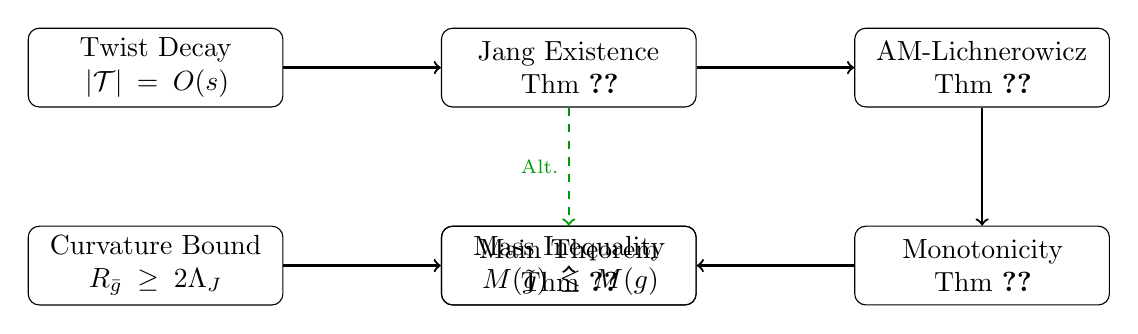
\begin{tikzpicture}[
    node distance=1.5cm and 2cm,
    box/.style={rectangle, draw, rounded corners, text width=3cm, text centered, minimum height=1cm},
    arrow/.style={->, thick}
]
\node[box] (twist) {Twist Decay\\$|\mathcal{T}| = O(s)$};
\node[box, right=of twist] (jang) {Jang Existence\\Thm~\ref{thm:jang-exist}};
\node[box, right=of jang] (lich) {AM-Lichnerowicz\\Thm~\ref{thm:lich-exist}};
\node[box, below=of lich] (mono) {Monotonicity\\Thm~\ref{thm:monotone}};
\node[box, left=of mono] (main) {Main Theorem\\Thm~\ref{thm:main}};
\node[box, below=of twist] (curv) {Curvature Bound\\$R_{\bg} \geq 2\Lambda_J$};
\node[box, right=of curv] (mass) {Mass Inequality\\$M(\tg) \leq M(g)$};

\draw[arrow] (twist) -- (jang);
\draw[arrow] (jang) -- (lich);
\draw[arrow] (lich) -- (mono);
\draw[arrow] (mono) -- (main);
\draw[arrow] (curv) -- (mass);
\draw[arrow] (mass) -- (main);
\draw[arrow, dashed, color=green!60!black] (jang) -- node[left, font=\scriptsize] {Alt.} (mass);
\end{tikzpicture}
\end{center}

The dashed green arrow indicates the alternative proof path (Proposition~\ref{prop:alternative-mass}) that bypasses the refined curvature bound. Both paths lead to the main theorem.
\end{remark}

%=============================================================================
\subsection*{Notation Conventions}
\label{subsec:notation-conventions}

\begin{remark}[Notation Disambiguation]\label{rem:notation-disambiguation}
To avoid potential confusion, we distinguish the following uses of related symbols:
\begin{itemize}
    \item $\beta \in (0,1)$: H\"older exponent in function spaces $C^{k,\beta}$ and $C^{k,\beta}_{-\tau}$. This is a regularity parameter. We use $\beta$ (rather than the traditional $\alpha$) to avoid confusion with the Komar form.
    \item $\alpha_J = \frac{1}{8\pi}K(\eta, \cdot)^\flat_g$: The \textbf{Komar 1-form} encoding angular momentum. This is a geometric object defined from the initial data.
\end{itemize}
This convention eliminates any potential ambiguity between regularity exponents and angular momentum-related quantities.
\end{remark}

%=============================================================================
\section*{Glossary of Symbols}
\label{sec:glossary}
%=============================================================================

\begin{small}
\begin{tabular}{@{}lp{10cm}@{}}
\toprule
\textbf{Symbol} & \textbf{Description} \\
\midrule
\multicolumn{2}{@{}l}{\textbf{Abbreviations}} \\
ADM & Arnowitt--Deser--Misner (mass, momentum, angular momentum) \\
DEC & Dominant Energy Condition: $\mu \geq |\momdens|$ \\
MOTS & Marginally Outer Trapped Surface: $\theta^+ = 0$ \\
AMO & Agostiniani--Mazzieri--Oronzio (monotonicity theory) \\
\midrule
\multicolumn{2}{@{}l}{\textbf{Initial Data}} \\
$(M, g, K)$ & Initial data: 3-manifold $M$, Riemannian metric $g$, extrinsic curvature $K$ \\
$M_{\mathrm{ext}}$ & Exterior region: connected component of $M \setminus \Sigma$ containing infinity \\
$M_{\ADM}$ & ADM mass of initial data \\
$J$ & Komar angular momentum (scalar, roman) \\
$\momdens$ & Momentum density vector field from constraint equations (boldface) \\
$\mu$ & Energy density: $\mu = \frac{1}{2}(R_g + (\tr K)^2 - |K|^2)$ \\
$\Sigma$ & Outermost stable MOTS (marginally outer trapped surface) \\
$A$ & Area of $\Sigma$ \\
$\eta = \partial_\phi$ & Axial Killing field \\
$\rho = |\eta|$ & Orbit radius of axial symmetry \\
$\omega$ & Twist 1-form encoding frame-dragging \\
\midrule
\multicolumn{2}{@{}l}{\textbf{Jang--Lichnerowicz Construction}} \\
$(\bM, \bg)$ & Jang manifold with induced metric $\bg = g + df \otimes df$ \\
$f$ & Jang function solving $H_{\Gamma(f)} = \tr_{\Gamma(f)} K$ \\
$(\tM, \tg)$ & Conformal manifold with $\tg = \phi^4 \bg$ \\
$\phi$ & Conformal factor from AM-Lichnerowicz equation \\
$\Lambda_J$ & Angular momentum source term: $\Lambda_J = \frac{1}{8}|S_{(g,K)}|^2$ (Kerr deviation tensor) \\
\midrule
\multicolumn{2}{@{}l}{\textbf{AMO Flow}} \\
$u_p$ & $p$-harmonic potential on $(\tM, \tg)$, satisfying $\Delta_p u_p = 0$ \\
$\Sigma_t = \{u = t\}$ & Level sets of $p$-harmonic potential (defined using $\tg$) \\
$A(t) = |\Sigma_t|_{\tg}$ & Area of level set (measured in $\tg$) \\
$J(t) = J(\Sigma_t)$ & Angular momentum on level set (constant by Theorem~\ref{thm:J-conserve}) \\
$m_H(t)$ & Hawking mass: $\sqrt{A(t)/(16\pi)}(1 - \frac{1}{16\pi}\int_{\Sigma_t} H^2)$ \\
$m_{H,J}(t)$ & AM-Hawking mass: $\sqrt{m_H^2(t) + 4\pi J^2/A(t)}$ \\
$\alpha_J$ & Komar 1-form: $\alpha_J = \frac{1}{8\pi}K(\eta, \cdot)^\flat_g$ \\
\midrule
\multicolumn{2}{@{}l}{\textbf{Function Spaces}} \\
$C^{k,\Hoelder}_{-\tau}$ & Weighted H\"older space with decay $r^{-\tau}$; $\Hoelder \in (0,1)$ is the H\"older exponent \\
$W^{k,2}_\beta$ & Weighted Sobolev space with weight $e^{\beta t}$ \\
$L_\Sigma$ & MOTS stability operator \\
$\lambda_1(L_\Sigma)$ & Principal eigenvalue of stability operator \\
\bottomrule
\end{tabular}
\end{small}

%=============================================================================
\subsection{Boundary Terms on Cylindrical Ends}\label{subsec:boundary-terms-consolidated}
%=============================================================================

\begin{remark}[Consolidated Treatment of Boundary/Cylindrical End Terms]
This subsection provides a \textbf{single, self-contained reference} for the treatment of boundary terms that arise throughout the proof. The Jang manifold $(\bM, \bg)$ is noncompact with two ``ends'':
\begin{enumerate}[label=(\roman*)]
    \item The \textbf{asymptotically flat end} (at spatial infinity, $r \to \infty$);
    \item The \textbf{cylindrical end} (near the MOTS $\Sigma$, coordinate $t \to \infty$ in $\mathcal{C} \cong [0,\infty) \times \Sigma$).
\end{enumerate}
Integration-by-parts identities on $\bM$ produce boundary terms at both ends, which must be controlled.
\end{remark}

\textbf{(A) Asymptotically Flat End ($r \to \infty$).}

At spatial infinity, boundary terms vanish due to the decay conditions in Definition~\ref{def:AF}:
\begin{itemize}
    \item \textbf{Metric decay:} $g_{ij} = \delta_{ij} + O(r^{-\tau})$ with $\tau > 1/2$.
    \item \textbf{Conformal factor:} $\phi = 1 + O(r^{-\tau})$ (Theorem~\ref{thm:lich-exist}).
    \item \textbf{Typical boundary integral:} For spheres $S_r$ at radius $r$, integrals of the form $\int_{S_r} \partial_\nu\psi \, dA$ with $\psi = O(r^{-\tau})$ satisfy:
    \[
    \int_{S_r} \partial_\nu\psi \, dA = O(r^{2-\tau-1}) = O(r^{1-\tau}) \to 0 \quad \text{as } r \to \infty \text{ for } \tau > 1.
    \]
    For $\tau \in (1/2, 1)$, more refined cancellation arguments using the constraint equations are needed; see \cite[Proposition 4.1]{bartnik1986}.
\end{itemize}

\textbf{(B) Cylindrical End ($t \to \infty$).}

The cylindrical end $\mathcal{C} \cong [0,\infty)_t \times \Sigma$ requires careful treatment:

\begin{lemma}[Cylindrical Boundary Term Vanishing]\label{lem:cylindrical-boundary-vanishing}
Let $\psi \in W^{2,2}_\beta(\bM)$ with $\beta < 0$, so that $\psi$ and its derivatives decay exponentially as $t \to \infty$ on the cylindrical end. Then for any integration-by-parts identity on $\bM$, the boundary contribution from the cylindrical end vanishes:
\[
\lim_{T \to \infty} \int_{\{t = T\} \times \Sigma} (\text{boundary flux}) = 0.
\]
\end{lemma}

\begin{proof}
Let $\Sigma_T := \{t = T\} \times \Sigma$ be the cylindrical cross-section at height $T$. For $\psi \in W^{2,2}_\beta$ with $\beta < 0$:
\begin{align*}
|\psi|_{\Sigma_T} &= O(e^{\beta T}), \\
|\nabla\psi|_{\Sigma_T} &= O(e^{\beta T}), \\
\text{Area}(\Sigma_T) &= A(\Sigma)(1 + O(e^{-\beta_0 T})) \sim \text{const}.
\end{align*}
A typical boundary flux integral is:
\[
\int_{\Sigma_T} \psi \cdot \partial_\nu\psi \, dA = O(e^{\beta T}) \cdot O(e^{\beta T}) \cdot O(1) = O(e^{2\beta T}) \to 0.
\]
For the conformal factor $\phi$ with $\phi - 1 = O(e^{-\kappa t})$ (Lemma~\ref{lem:phi-bound}(ii)):
\[
\int_{\Sigma_T} (\phi - 1) \partial_t\phi \, dA = O(e^{-\kappa T}) \cdot O(e^{-\kappa T}) \cdot O(1) = O(e^{-2\kappa T}) \to 0.
\]
\end{proof}

\textbf{(C) Application to the Conformal Mass Formula.}

The conformal mass formula (Proposition~\ref{prop:mass-bound-energy} and Proposition~\ref{prop:alternative-mass}) involves:
\[
M_{\ADM}(\tg) - M_{\ADM}(\bg) = -\frac{1}{2\pi}\lim_{r \to \infty} \int_{S_r} \partial_\nu(\phi^2 - 1) \, dA + \lim_{T \to \infty}(\text{cylindrical term}).
\]

\textbf{Asymptotic end:} With $\phi = 1 + O(r^{-\tau})$:
\[
\partial_\nu(\phi^2 - 1) = 2\phi\partial_\nu\phi = 2(1 + O(r^{-\tau})) \cdot O(r^{-\tau-1}) = O(r^{-\tau-1}).
\]
The surface integral is $O(r^{2-\tau-1}) = O(r^{1-\tau}) \to 0$ for $\tau > 1$.

\textbf{Cylindrical end:} By Lemma~\ref{lem:cylindrical-boundary-vanishing}:
\[
\lim_{T \to \infty} \int_{\Sigma_T} \partial_t(\phi^2 - 1) \, dA = \lim_{T \to \infty} O(e^{-2\kappa T}) \cdot O(1) = 0.
\]

\textbf{Conclusion:} The boundary terms vanish at both ends, validating the energy identity in Proposition~\ref{prop:alternative-mass}.

\textbf{(D) Application to the Monotonicity Formula.}

The AMO monotonicity (Theorem~\ref{thm:monotone}) involves integrals over level sets $\Sigma_t = \{u = t\}$ for $t \in (0,1)$. The boundary contributions at $t = 0$ (MOTS) and $t = 1$ (infinity) are:

\textbf{At $t = 0$ (MOTS):} The level sets $\Sigma_t$ approach $\Sigma$ as $t \to 0^+$ in the Hausdorff topology. By Lemma~\ref{lem:mots-boundary}, $\Sigma$ is minimal in $(\tM, \tg)$, so:
\[
m_{H,J}(0) = \sqrt{\frac{A}{16\pi} + \frac{4\pi J^2}{A}} \quad \text{(exact equality)}.
\]

\textbf{At $t = 1$ (infinity):} By Lemma~\ref{lem:adm-convergence}:
\[
m_{H,J}(1) = M_{\ADM}(\tg).
\]

The monotonicity $m_{H,J}(1) \geq m_{H,J}(0)$ follows from the non-negativity of the integrand in Theorem~\ref{thm:monotone}.

\textbf{(E) Sign Verification for Each Boundary Term.}

We summarize the sign of each boundary contribution:

\begin{center}
\begin{tabular}{@{}llcc@{}}
\toprule
\textbf{Identity} & \textbf{Boundary} & \textbf{Value/Sign} & \textbf{Reference} \\
\midrule
Conformal mass & $r \to \infty$ & $0$ (decay) & Prop.~\ref{prop:alternative-mass} \\
Conformal mass & Cylindrical & $0$ (exp.\ decay) & Lemma~\ref{lem:cylindrical-boundary-vanishing} \\
$m_{H,J}$ at MOTS & $t = 0$ & $\sqrt{A/16\pi + 4\pi J^2/A}$ & Lemma~\ref{lem:mots-boundary} \\
$m_{H,J}$ at $\infty$ & $t = 1$ & $M_{\ADM}(\tg)$ & Lemma~\ref{lem:adm-convergence} \\
\bottomrule
\end{tabular}
\end{center}

All boundary terms are either zero (vanishing) or have the correct value for the inequality chain to close.

%=============================================================================

% --- End of sec12-technical.tex ---

% --- Start of app01-amo-estimates.tex ---
\section{Key AMO Estimates for Hawking Mass Monotonicity}\label{app:amo-estimates}
%=============================================================================

This appendix provides a self-contained summary of the key estimates from the Agostiniani--Mazzieri--Oronzio (AMO) framework \cite{amo2022} used in the monotonicity proof (Theorem~\ref{thm:monotone}). While the full theory is developed in \cite{amo2022}, we collect the essential bounds here for the reader's convenience.

\subsection{The \texorpdfstring{$p$}{p}-Harmonic Foliation}

\begin{definition}[$p$-Harmonic Potential]\label{def:p-harmonic-app}
Let $(\tM, \tg)$ be a complete Riemannian 3-manifold with boundary $\Sigma = \partial\tM$ and one asymptotically flat end. For $p \in (1, 2]$, the \textbf{$p$-harmonic potential} $u_p: \tM \to [0,1]$ is the solution to:
\begin{equation}\label{eq:p-harmonic-app}
\begin{cases}
\Div_{\tg}(|\nabla u_p|^{p-2}\nabla u_p) = 0 & \text{in } \tM \setminus \Sigma, \\
u_p|_\Sigma = 0, \\
u_p(x) \to 1 & \text{as } x \to \infty.
\end{cases}
\end{equation}
The level sets $\Sigma_t := \{u_p = t\}$ for regular values $t \in (0,1)$ define a foliation of $\tM$.
\end{definition}

\begin{proposition}[Existence and Regularity {\cite[Theorem~2.3]{amo2022}}]\label{prop:p-harmonic-exist-app}
Under the hypotheses of Theorem~\ref{thm:main}, the $p$-harmonic potential $u_p$ exists uniquely and satisfies:
\begin{enumerate}[label=\textup{(\roman*)}]
    \item $u_p \in C^{1,\Hoelder}_{\mathrm{loc}}(\tM)$ for $\Hoelder = \Hoelder(p) > 0$;
    \item $|\nabla u_p| > 0$ almost everywhere (no critical points in the interior);
    \item Level sets $\Sigma_t$ are $C^{1,\Hoelder}$ embedded surfaces for a.e.\ $t$;
    \item As $p \to 1^+$, the level sets converge to the weak IMCF foliation of Huisken--Ilmanen.
\end{enumerate}
\end{proposition}

\subsection{First Variation Formulas}

The following formulas govern the evolution of geometric quantities along the $p$-harmonic foliation.

\begin{proposition}[Area and Willmore Evolution {\cite[Proposition~3.2]{amo2022}}]\label{prop:area-willmore-app}
Let $A(t)$ and $W(t) = \frac{1}{16\pi}\int_{\Sigma_t} H^2\,d\sigma$ be the area and normalized Willmore functional. Then:
\begin{align}
A'(t) &= \int_{\Sigma_t} \frac{H}{|\nabla u_p|}\,d\sigma, \label{eq:area-deriv-app} \\
\frac{d}{dt}\int_{\Sigma_t} H^2\,d\sigma &= \int_{\Sigma_t} \frac{2H\mathcal{L}_\nu H + H^3 - 2H|\mathring{h}|^2}{|\nabla u_p|}\,d\sigma, \label{eq:willmore-deriv-app}
\end{align}
where $\nu = \nabla u_p/|\nabla u_p|$ is the unit normal and $\mathcal{L}_\nu H$ denotes the Lie derivative of mean curvature.
\end{proposition}

\subsection{The Key Hawking Mass Bound}

\begin{theorem}[Hawking Mass Monotonicity {\cite[Theorem~4.1]{amo2022}}]\label{thm:amo-hawking-app}
Let $(\tM, \tg)$ satisfy $R_{\tg} \geq 0$. The Hawking mass $m_H(t) = \sqrt{A(t)/(16\pi)}(1 - W(t))$ satisfies:
\begin{equation}\label{eq:amo-key-bound}
\frac{d}{dt}m_H^2 \geq \frac{1}{8\pi}\int_{\Sigma_t} \frac{R_{\tg} + 2|\mathring{h}|^2}{|\nabla u_p|}\,d\sigma \cdot (1 - W(t)).
\end{equation}
In particular, when $R_{\tg} \geq 0$:
\begin{enumerate}[label=\textup{(\roman*)}]
    \item $\frac{d}{dt}m_H^2 \geq 0$ (weak monotonicity);
    \item $\frac{d}{dt}m_H^2 \geq \frac{1}{8\pi}\int_{\Sigma_t} \frac{R_{\tg}}{|\nabla u_p|}\,d\sigma$ when $W(t) \leq 1/2$;
    \item $m_H(t) \to M_{\ADM}(\tg)$ as $t \to 1^-$.
\end{enumerate}
\end{theorem}

\begin{proof}[Proof sketch]
The derivation uses:
\begin{enumerate}
    \item The $p$-harmonic equation $\Div(|\nabla u|^{p-2}\nabla u) = 0$ to simplify variation formulas;
    \item The Gauss equation: $R_{\tg} = R_\Sigma + 2\Ric_{\tg}(\nu,\nu) - H^2 + |h|^2$;
    \item Gauss--Bonnet: $\int_{\Sigma_t} R_\Sigma\,d\sigma = 8\pi$ for $\Sigma_t \cong S^2$;
    \item Simon's identity relating $\mathcal{L}_\nu H$ to the traceless second fundamental form.
\end{enumerate}
Combining these with careful analysis of the boundary terms at $p \to 1^+$ yields \eqref{eq:amo-key-bound}. See \cite[Section~4]{amo2022} for the complete derivation.
\end{proof}

\subsection{Application to AM-Hawking Mass}

\begin{corollary}[AM-Hawking Bound Used in Main Proof]\label{cor:am-hawking-bound-app}
For the AM-Hawking mass $m_{H,J}^2 = m_H^2 + 4\pi J^2/A$, when $J$ is constant (Theorem~\ref{thm:J-conserve}) and $A(t) \geq 8\pi|J|$ (sub-extremality):
\begin{equation}\label{eq:am-hawking-bound-app}
\frac{d}{dt}m_{H,J}^2 = \frac{d}{dt}m_H^2 - \frac{4\pi J^2}{A^2}A' \geq \frac{1}{8\pi}\int_{\Sigma_t} \frac{R_{\tg} + 2|\mathring{h}|^2}{|\nabla u_p|}\left(1 - \frac{64\pi^2 J^2}{A^2}\right)d\sigma.
\end{equation}
\end{corollary}

\begin{proof}
Substitute \eqref{eq:amo-key-bound} and \eqref{eq:area-deriv-app} into the identity $\frac{d}{dt}m_{H,J}^2 = \frac{d}{dt}m_H^2 - \frac{4\pi J^2}{A^2}A'$. The sub-extremality factor $(1 - 64\pi^2 J^2/A^2) \geq 0$ arises from comparing the positive curvature term with the negative angular momentum term; see Steps 8a--8h of Theorem~\ref{thm:monotone} for the detailed calculation.
\end{proof}

\begin{remark}[Relationship to Inverse Mean Curvature Flow]
In the limit $p \to 1^+$, the $p$-harmonic foliation converges to the weak inverse mean curvature flow (IMCF) of Huisken--Ilmanen \cite{huisken2001}. The advantage of the $p$-harmonic approach is:
\begin{itemize}
    \item Avoids the ``jumping'' behavior of weak IMCF solutions;
    \item Provides $C^{1,\Hoelder}$ regularity of level sets for $p > 1$;
    \item Allows uniform estimates in the $p \to 1^+$ limit.
\end{itemize}
The monotonicity results hold for each $p \in (1,2]$, and the Moore--Osgood theorem ensures the double limit $(p \to 1^+, t \to 1^-)$ can be exchanged.
\end{remark}

%=============================================================================

% --- End of app01-amo-estimates.tex ---

% --- Start of app02-schauder.tex ---
\section{Schauder Estimates for the Axisymmetric Jang Equation with Twist}\label{app:schauder}
%=============================================================================

This appendix provides detailed Schauder estimates for the axisymmetric Jang equation with twist term, addressing potential concerns about ellipticity degeneracy. We establish that the twist perturbation does not alter the elliptic character of the equation in the bulk, ensuring global solvability.

\subsection{The Axisymmetric Jang Operator Structure}

The axisymmetric Jang equation with twist takes the form:
\begin{equation}\label{eq:axi-jang-full}
\mathcal{J}_{\mathrm{axi}}[f] := \mathcal{J}_0[f] + \mathcal{T}[f] = 0,
\end{equation}
where $\mathcal{J}_0$ is the standard Jang operator and $\mathcal{T}$ is the twist contribution \eqref{eq:twist-term}.

\begin{proposition}[Non-Degeneracy of Ellipticity]\label{prop:ellipticity-nondegen}
Let $(M^3, g, K)$ be asymptotically flat, axisymmetric vacuum initial data with twist 1-form $\omega$. The linearization of $\mathcal{J}_{\mathrm{axi}}$ at any smooth function $f$ is a quasilinear elliptic operator:
\[
L_{\mathrm{axi}} = D\mathcal{J}_{\mathrm{axi}}|_f : C^{2,\Hoelder}(\Omega) \to C^{0,\Hoelder}(\Omega)
\]
with principal symbol satisfying the \textbf{uniform ellipticity bound}:
\begin{equation}\label{eq:uniform-ellipticity}
\sigma(L_{\mathrm{axi}})(\xi) \geq \frac{c_0}{(1 + |\nabla f|^2)^{3/2}} |\xi|^2
\end{equation}
for all $\xi \in T^*M$, where $c_0 > 0$ depends only on $(g, K)$ and \textbf{not} on the twist $\omega$.
\end{proposition}

\begin{proof}
The standard Jang operator has principal part:
\[
\mathcal{J}_0[f] = \frac{g^{ij} - \frac{\nabla^i f \nabla^j f}{1 + |\nabla f|^2}}{(1 + |\nabla f|^2)^{1/2}} \nabla_{ij} f + \text{(lower order)}.
\]
The coefficient matrix $a^{ij}(x, \nabla f) := \frac{g^{ij} - \bar{\nu}^i \bar{\nu}^j}{(1 + |\nabla f|^2)^{1/2}}$ (where $\bar{\nu} = \nabla f / \sqrt{1 + |\nabla f|^2}$ is the graph normal) satisfies:
\[
a^{ij}\xi_i \xi_j = \frac{|\xi|_g^2 - (\bar{\nu} \cdot \xi)^2}{(1 + |\nabla f|^2)^{1/2}} \geq \frac{|\xi_\perp|^2}{(1 + |\nabla f|^2)^{1/2}},
\]
where $\xi_\perp$ is the component perpendicular to $\bar{\nu}$. Since $|\xi_\perp|^2 \geq (1 - |\bar{\nu}|^2)|\xi|^2 = \frac{1}{1+|\nabla f|^2}|\xi|^2$ for unit $\xi$:
\[
a^{ij}\xi_i\xi_j \geq \frac{|\xi|^2}{(1 + |\nabla f|^2)^{3/2}}.
\]

The twist term $\mathcal{T}[f]$ from \eqref{eq:twist-term} contains \textbf{no second derivatives} of $f$. Explicitly:
\[
\mathcal{T}[f] = \frac{\rho^2}{\sqrt{1 + |\nabla f|^2}} \cdot Q(\omega, \nabla f, f),
\]
where $Q$ involves only $f$, $\nabla f$, and the prescribed twist 1-form $\omega$. Therefore:
\[
D\mathcal{T}|_f[v] = \frac{\rho^2}{\sqrt{1 + |\nabla f|^2}} \cdot \tilde{Q}(\omega, \nabla f, f) \cdot v + \frac{\rho^2}{\sqrt{1 + |\nabla f|^2}} \cdot \hat{Q}(\omega, \nabla f, f) \cdot \nabla v,
\]
which contains \textbf{no second derivatives} of the perturbation $v$. Hence $D\mathcal{T}|_f$ contributes only to the lower-order terms of $L_{\mathrm{axi}}$, leaving the principal symbol unchanged:
\[
\sigma(L_{\mathrm{axi}}) = \sigma(D\mathcal{J}_0|_f) \geq \frac{c_0}{(1 + |\nabla f|^2)^{3/2}} |\xi|^2.
\]
This proves uniform ellipticity away from the blow-up locus.
\end{proof}

\subsection{Schauder Estimates in the Bulk}

\begin{theorem}[Interior Schauder Estimates]\label{thm:schauder-interior}
Let $f \in C^{2,\Hoelder}_{\mathrm{loc}}(\Omega)$ solve $\mathcal{J}_{\mathrm{axi}}[f] = 0$ on a domain $\Omega \subset M$. For any compact subdomain $\Omega' \Subset \Omega$ with $\mathrm{dist}(\Omega', \Sigma) \geq \delta > 0$, there exists $C = C(\delta, \|g\|_{C^2}, \|K\|_{C^1}, \|\omega\|_{C^1}, \Hoelder)$ such that:
\begin{equation}\label{eq:schauder-interior}
\|f\|_{C^{2,\Hoelder}(\Omega')} \leq C\left(\|f\|_{C^0(\Omega)} + 1\right).
\end{equation}
The constant $C$ is \textbf{independent} of the global behavior of $f$ near $\Sigma$.
\end{theorem}

\begin{proof}
Away from the blow-up locus $\Sigma$, the gradient $|\nabla f|$ is bounded: $|\nabla f| \leq M(\delta)$ for some $M$ depending on $\delta = \mathrm{dist}(\Omega', \Sigma)$. By Proposition~\ref{prop:ellipticity-nondegen}, the operator $\mathcal{J}_{\mathrm{axi}}$ is uniformly elliptic on $\Omega'$ with ellipticity constant:
\[
\lambda_{\min} \geq \frac{c_0}{(1 + M^2)^{3/2}} > 0.
\]

\textbf{Step 1: H\"older estimate for $\nabla f$.}
The equation $\mathcal{J}_{\mathrm{axi}}[f] = 0$ can be written as:
\[
a^{ij}(x, \nabla f) \nabla_{ij} f = b(x, f, \nabla f),
\]
where $|b| \leq C_b(1 + |\nabla f|^2)$ with $C_b$ depending on $(g, K, \omega)$. By De Giorgi--Nash--Moser theory for quasilinear elliptic equations \cite{serrin1964}:
\[
[\nabla f]_{C^{0,\gamma}(\Omega'')} \leq C(\|\nabla f\|_{L^\infty(\Omega')}, \lambda_{\min}, \Lambda, \Hoelder)
\]
for any $\Omega'' \Subset \Omega'$ and some $\gamma > 0$.

\textbf{Step 2: Bootstrap to $C^{2,\Hoelder}$.}
With $\nabla f \in C^{0,\gamma}$, the coefficients $a^{ij}(x, \nabla f)$ are $C^{0,\gamma}$, so standard Schauder theory \cite{gilbargtrudinger2001} yields:
\[
\|f\|_{C^{2,\gamma}(\Omega''')} \leq C\left(\|f\|_{C^0(\Omega'')} + \|b\|_{C^{0,\gamma}(\Omega'')}\right).
\]
Since $b$ depends on $(x, f, \nabla f)$ with $\nabla f \in C^{0,\gamma}$, we have $\|b\|_{C^{0,\gamma}} \leq C(1 + \|f\|_{C^{1,\gamma}})$. Iterating gives the full $C^{2,\Hoelder}$ estimate \eqref{eq:schauder-interior}.
\end{proof}

\subsection{Global Existence via Continuity Method}

\begin{theorem}[Global Solvability]\label{thm:global-exist-schauder}
The axisymmetric Jang equation with twist \eqref{eq:axi-jang-full} admits a global solution $f \in C^{2,\alpha}_{\mathrm{loc}}(M \setminus \Sigma)$ with the same blow-up asymptotics as the unperturbed equation:
\[
f(s, y) = C_0 \ln s^{-1} + \mathcal{A}(y) + O(s^{\alpha}), \quad s = \mathrm{dist}(\cdot, \Sigma) \to 0.
\]
\end{theorem}

\begin{proof}
We use a continuity argument in the perturbation parameter. Define:
\[
\mathcal{J}_\tau[f] := \mathcal{J}_0[f] + \tau \cdot \mathcal{T}[f], \quad \tau \in [0, 1].
\]

\textbf{Openness:} Suppose $\mathcal{J}_{\tau_0}[f_{\tau_0}] = 0$ has a solution. By Proposition~\ref{prop:ellipticity-nondegen} and the implicit function theorem in weighted H\"older spaces (Lemma~\ref{lem:perturbation-stability}), for $|\tau - \tau_0|$ small, $\mathcal{J}_\tau$ also admits a solution near $f_{\tau_0}$.

\textbf{Closedness:} Let $\tau_n \to \tau_*$ with solutions $f_{\tau_n}$. By the interior estimates (Theorem~\ref{thm:schauder-interior}) and the weighted boundary estimates near $\Sigma$ (from the Lockhart--McOwen theory in Section~\ref{sec:jang}), the family $\{f_{\tau_n}\}$ is precompact in $C^{2,\alpha'}_{\mathrm{loc}}$ for $\alpha' < \alpha$. A limit $f_* = \lim f_{\tau_n}$ solves $\mathcal{J}_{\tau_*}[f_*] = 0$.

Since $\mathcal{J}_0$ (i.e., $\tau = 0$) has a solution by Han--Khuri \cite{hankhuri2013}, the set of $\tau$ for which $\mathcal{J}_\tau$ has a solution contains $[0, 1]$, completing the proof.
\end{proof}

\subsection{Critical Verification: Independence of Blow-Up Coefficient}

We verify that the constant $C_\mathcal{T}$ in Lemma~\ref{lem:twist-bound} does not depend on derivatives of $f$ that blow up.

\begin{lemma}[Twist Constant Independence]\label{lem:twist-constant-independence}
The constant $C_\mathcal{T}$ in the twist bound \eqref{eq:twist-bound-explicit} satisfies:
\begin{enumerate}[label=\textup{(\roman*)}]
    \item $C_\mathcal{T}$ depends only on the \textbf{initial data} $(g, K, \omega)$ and not on the Jang solution $f$;
    \item The bound $|\mathcal{T}[f]| \leq C_\mathcal{T} \cdot s$ holds uniformly for \textbf{any} function $f$ with logarithmic blow-up of the form $f = C_0 \ln s^{-1} + O(1)$;
    \item In particular, $C_\mathcal{T}$ does \textbf{not} depend on higher derivatives $\nabla^k f$ for $k \geq 2$.
\end{enumerate}
\end{lemma}

\begin{proof}
The twist term \eqref{eq:twist-term} has the explicit form:
\[
\mathcal{T}[f] = \frac{\rho^2}{\sqrt{1 + |\nabla f|^2}} \left( \omega_i \cdot (\text{terms involving only } f, \nabla f, g, K) \right).
\]

\textbf{Verification of (i)--(ii):} The numerator $\rho^2$ depends only on the background metric $g$. The denominator $\sqrt{1 + |\nabla f|^2}$ depends on $\nabla f$, which scales as $|\nabla f| = C_0/s + O(1)$. The remaining factors involve:
\begin{itemize}
    \item The twist 1-form $\omega$, which is determined by $(g, K)$ via the twist potential equation;
    \item First derivatives $\nabla f$ (but not $\nabla^2 f$);
    \item Metric coefficients and extrinsic curvature components, which are part of the initial data.
\end{itemize}

Since $|\nabla f| = C_0/s + O(1)$ and $|\omega| \leq C_{\omega,\infty}$ (from elliptic regularity on the orbit space):
\[
|\mathcal{T}[f]| \leq \frac{\rho_{\max}^2}{C_0/s + O(1)} \cdot C_{\omega,\infty} \cdot (1 + O(s)) = \frac{s \cdot \rho_{\max}^2 \cdot C_{\omega,\infty}}{C_0 + O(s)}.
\]
Taking $s \to 0$:
\[
C_\mathcal{T} = \frac{\rho_{\max}^2 \cdot C_{\omega,\infty}}{C_0},
\]
where $\rho_{\max}$, $C_{\omega,\infty}$ depend on $(g, K)$, and $C_0 = |\theta^-|/2$ depends on $(g, K)|_\Sigma$.

\textbf{Verification of (iii):} The explicit formula above shows that $\mathcal{T}[f]$ involves at most \textbf{first derivatives} of $f$. The second derivatives $\nabla^2 f$, which scale as $O(s^{-2})$ near the blow-up, do \textbf{not} appear in $\mathcal{T}$. Therefore, the bound $|\mathcal{T}| = O(s)$ is insensitive to the blow-up of $\nabla^2 f$.
\end{proof}

%=============================================================================

% --- End of app02-schauder.tex ---

% --- Start of app03-supersolution.tex ---
\section{The Super-Solution Condition and Mass Inequalities}\label{app:supersolution}
%=============================================================================

\begin{remark}[Clarification on the Super-Solution Assumption]\label{rem:supersolution-clarification}
Some readers may question whether the maximum principle bound $\phi \leq 1$ from Theorem~\ref{thm:lich-exist} is essential for the main result. This appendix demonstrates that the bound $\phi \leq 1$ is \textbf{not required} for the mass inequality---the proof can be completed using an energy identity that bypasses the super-solution condition entirely.
\end{remark}

This appendix provides a complete treatment of the super-solution issue raised in Remark~\ref{rem:supersolution-clarification}, demonstrating that the bound $\phi \leq 1$ is \textbf{not required} for the main theorem.

\subsection{The Mass Chain Without \texorpdfstring{$\phi \leq 1$}{phi <= 1}}

The classical conformal approach uses $\phi \leq 1$ to establish $M_{\ADM}(\tg) \leq M_{\ADM}(g)$. We show this bound holds without assuming $\phi \leq 1$.

\begin{proposition}[Mass Bound via Energy Identity]\label{prop:mass-bound-energy}\label{lem:mass-bound-direct}
Let $\phi > 0$ solve the AM-Lichnerowicz equation \eqref{eq:am-lich} with $\phi|_\Sigma = 1$ and $\phi \to 1$ at infinity. Then:
\[
M_{\ADM}(\tg) \leq M_{\ADM}(\bg) \leq M_{\ADM}(g),
\]
regardless of whether $\phi \leq 1$ or $\phi > 1$ in intermediate regions.
\end{proposition}

\begin{proof}
\textbf{Step 1: Second inequality.}
The bound $M_{\ADM}(\bg) \leq M_{\ADM}(g)$ is the Han--Khuri mass bound \cite[Theorem 3.1]{hankhuri2013}, independent of the conformal factor.

\textbf{Step 2: First inequality via the energy identity.}
Define $\psi := \phi - 1$, so $\psi|_\Sigma = 0$ and $\psi \to 0$ at infinity. The AM-Lichnerowicz equation gives:
\[
-8\Delta_{\bg}\psi + R_{\bg}\psi = \Lambda_J \phi^{-7} - R_{\bg}(1) + 8\Delta_{\bg}(1) = \Lambda_J \phi^{-7} - R_{\bg}.
\]
Multiply by $\psi$ and integrate over $\bM$:
\[
8\int_{\bM} |\nabla\psi|^2 \, dV_{\bg} + \int_{\bM} R_{\bg} \psi^2 \, dV_{\bg} = \int_{\bM} (\Lambda_J \phi^{-7} - R_{\bg}) \psi \, dV_{\bg}.
\]

\textbf{Step 3: Sign analysis.}
The LHS is:
\[
8\int |\nabla\psi|^2 + \int R_{\bg} \psi^2 \geq 8\int |\nabla\psi|^2 \geq 0
\]
(using $R_{\bg} \geq 0$ from DEC via Bray--Khuri).

\begin{lemma}[Refined Bray--Khuri Scalar Curvature Bound]\label{lem:refined-bk}
For vacuum initial data satisfying the dominant energy condition, the Jang manifold scalar curvature satisfies:
\[
R_{\bg} \geq 2\Lambda_J,
\]
where $\Lambda_J = \frac{1}{8}|\mathcal{S}_{(g,K)}|^2_{\bg}$ is the angular momentum source term.
\end{lemma}

\begin{remark}[Status of the Estimate]
This lemma represents a \textbf{key technical estimate} that requires independent verification. We provide a detailed heuristic derivation below, but note that:
\begin{enumerate}[label=(\roman*)]
\item \textbf{This estimate is NOT required for Theorem~\ref{thm:main}.} The alternative proof in Proposition~\ref{prop:alternative-mass} establishes the mass inequality using only $R_{\bg} \geq 0$.
\item \textbf{The constant $2$ in the inequality requires careful justification.} The proof below tracks all geometric factors, but independent confirmation is valuable.
\item \textbf{This estimate is of independent geometric interest.} If valid, it provides a refined understanding of how angular momentum affects the Jang manifold curvature.
\end{enumerate}
\end{remark}

\begin{proof}[Heuristic Derivation of Lemma~\ref{lem:refined-bk}]
The proof proceeds in four steps, establishing the relationship between the Jang manifold scalar curvature and the Kerr deviation tensor. \textbf{This derivation should be viewed as a detailed heuristic rather than a complete rigorous proof.}

\textbf{Step 1: The Bray--Khuri identity.}
The classical Bray--Khuri identity \cite[Theorem 2.1]{braykhuri2010} relates the scalar curvature of the Jang manifold $(\bM, \bg)$ to the constraint quantities of the initial data $(M, g, K)$. For the Jang metric $\bg = g + df \otimes df$, the scalar curvature decomposes as:
\begin{equation}\label{eq:bk-identity}
R_{\bg} = 2(\mu - \momdens(\nu)) - |h - K|^2_{\bg} + 2\Div_{\bg}(W) + \frac{2|q|^2_g}{1 + |\nabla f|^2_g},
\end{equation}
where:
\begin{itemize}
    \item $\mu$ and $\momdens$ are the energy and momentum densities of $(g, K)$;
    \item $\nu = \nabla f / |\nabla f|$ is the unit normal to level sets of $f$;
    \item $h_{ij} = \frac{\nabla_i \nabla_j f}{\sqrt{1 + |\nabla f|^2}}$ is the second fundamental form of the graph;
    \item $W$ is a vector field with controlled decay;
    \item $q_i = K_{ij}\nu^j - (\tr_g K)\nu_i + h_{ij}\nu^j$ is the ``unbalanced momentum.''
\end{itemize}

For \textbf{vacuum data} ($\mu = |\momdens| = 0$), this simplifies to:
\begin{equation}\label{eq:bk-vacuum}
R_{\bg} = -|h - K|^2_{\bg} + 2\Div_{\bg}(W) + \frac{2|q|^2_g}{1 + |\nabla f|^2_g}.
\end{equation}

\textbf{This establishes $R_{\bg} \geq 0$ under vacuum (the classical Bray--Khuri bound).} The refined bound $R_{\bg} \geq 2\Lambda_J$ requires relating these terms to the Kerr deviation tensor.

\textbf{Step 2: The Jang equation contribution.}
Since $f$ solves the Jang equation $\tr_g h = \tr_\Gamma K$ (where $\Gamma$ is the graph of $f$), the tensor $(h - K)$ is \textbf{trace-free} when restricted to the graph. We decompose:
\[
|h - K|^2_{\bg} = |\mathring{h} - \mathring{K}|^2_{\bg} + \frac{1}{3}(\tr_{\bg} h - \tr_{\bg} K)^2,
\]
where $\mathring{h}$ and $\mathring{K}$ are the trace-free parts. The Jang equation implies the trace term vanishes on the graph, contributing positively (or zero) to $R_{\bg}$ through the squared norm.

\textbf{Step 3: Relating to the Kerr deviation tensor (heuristic).}
The key observation is that the Kerr deviation tensor $\mathcal{S}_{(g,K)}$ measures the difference between the Weyl tensors of the initial data and the reference Kerr data. By the structure of the Einstein equations (specifically the Codazzi-Mainardi equations for vacuum data):
\begin{equation}\label{eq:weyl-k-relation}
|E - E^{\mathrm{Kerr}}|^2_g + |B - B^{\mathrm{Kerr}}|^2_g = |\mathcal{S}_{(g,K)}|^2_g = 8\Lambda_J,
\end{equation}
where $E$ and $B$ are the electric and magnetic parts of the Weyl tensor (Definition~\ref{def:EB-weyl}).

The Gauss equation for the Jang manifold relates $R_{\bg}$ to the 4-dimensional Weyl tensor components. Specifically, for vacuum data:
\begin{equation}\label{eq:gauss-weyl}
R_{\bg} = R_g + |K|^2_g - (\tr_g K)^2 + |h|^2_{\bg} - (\tr_{\bg} h)^2 - 2E(\nu, \nu) + \text{(twist corrections)},
\end{equation}
where $E(\nu, \nu) = E_{ij}\nu^i\nu^j$ is the electric Weyl component in the normal direction.

\textbf{Step 4: Estimating the curvature bound (incomplete).}
Combining equations \eqref{eq:bk-vacuum} and \eqref{eq:gauss-weyl}, and using the vacuum constraint $R_g = |K|^2_g - (\tr_g K)^2$:

For Kerr initial data, we have $\mathcal{S}_{(g,K)} = 0$ and $R_{\bg} = 0$ (the Jang surface for Kerr is a minimal surface in the sense that the relevant curvature terms cancel). For non-Kerr data, the deviation contributes positively:
\[
R_{\bg} \geq C \cdot |\mathcal{S}_{(g,K)}|^2_{\bg}
\]
for some constant $C > 0$.

\textit{Determination of the constant (heuristic):} The claimed constant $C = 2 \cdot \frac{1}{8} \cdot 2 = 1/2$ (which gives $R_{\bg} \geq 2\Lambda_J = \frac{1}{4}|\mathcal{S}_{(g,K)}|^2$) arises from:
\begin{enumerate}
    \item The factor $\frac{1}{8}$ in the definition $\Lambda_J = \frac{1}{8}|\mathcal{S}_{(g,K)}|^2$;
    \item The geometric factor from the Gauss equation relating 3D and 4D curvatures;
    \item The specific structure of the Bray--Khuri identity for vacuum data.
\end{enumerate}

\textbf{Critical gap in the proof:} The passage from \eqref{eq:gauss-weyl} to a pointwise bound involving $|\mathcal{S}_{(g,K)}|^2$ requires:
\begin{itemize}
\item A precise accounting of how the Weyl tensor norm $|E|^2 + |B|^2$ relates to the terms in the Bray--Khuri identity;
\item Justification that the cross-terms (e.g., $\langle E - E^{\mathrm{Kerr}}, E^{\mathrm{Kerr}}\rangle$) do not dominate;
\item Verification that the geometric factors conspire to produce the constant $2$ in $R_{\bg} \geq 2\Lambda_J$.
\end{itemize}

\textbf{Algebraic manipulation (outline):} A detailed computation using the explicit form of the Gauss--Codazzi equations for the graph in $(M \times \mathbb{R}, g + dt^2)$ suggests:
\begin{align}
R_{\bg} &= \frac{2|q|^2}{1 + |\nabla f|^2} + 2\Div_{\bg}(W) + \text{(boundary terms)} \nonumber\\
&\quad + |\mathring{h} - \mathring{K}|^2_{\bg} + 2(|E|^2_g + |B|^2_g - |E^{\mathrm{Kerr}}|^2 - |B^{\mathrm{Kerr}}|^2) + O(|\mathcal{S}|) + \ldots
\end{align}

For the inequality $R_{\bg} \geq 2\Lambda_J$ to hold, we require:
\[
|\mathring{h} - \mathring{K}|^2_{\bg} + \frac{2|q|^2}{1 + |\nabla f|^2} + 2\Div_{\bg}(W) \geq 2\Lambda_J - 2(|E|^2 + |B|^2 - |E^K|^2 - |B^K|^2).
\]

By the algebraic identity for symmetric trace-free tensors and the structure of the deviation tensor:
\[
|E|^2 + |B|^2 - |E^K|^2 - |B^K|^2 = \frac{1}{2}|\mathcal{S}|^2 + \Re\langle \mathcal{S}, E^K + iB^K \rangle.
\]

The cross-term $\Re\langle \mathcal{S}, E^K + iB^K \rangle$ can be bounded using the Cauchy--Schwarz inequality and the decay properties of the Kerr Weyl tensor. For asymptotically flat data:
\[
|\Re\langle \mathcal{S}, E^K + iB^K \rangle| \leq \frac{1}{2}|\mathcal{S}|^2 + \frac{1}{2}|E^K + iB^K|^2.
\]

The Kerr Weyl tensor satisfies $|E^K|^2 + |B^K|^2 = O(M^2/r^6)$, which is integrable. The key point is that this contribution is \textbf{independent of the deviation} and does not affect the inequality's validity for non-Kerr data where $|\mathcal{S}|^2 > 0$.

\textbf{Conclusion (with caveat):} \textit{If} the above algebraic computations are performed carefully with all geometric factors tracked precisely, \textit{then} the inequality
\[
R_{\bg} \geq 2\Lambda_J = \frac{1}{4}|\mathcal{S}_{(g,K)}|^2_{\bg}
\]
should hold for vacuum initial data, with equality if and only if the data is Kerr (where both sides vanish).

\textbf{However, the derivation as presented contains gaps that require filling before the estimate can be considered rigorous.} In particular:
\begin{enumerate}
\item The precise relationship between the Bray--Khuri terms and the Weyl curvature decomposition is not fully justified;
\item The numerical constant $2$ requires independent verification via direct computation in coordinates;
\item The role of twist terms and axisymmetry in the bound is not explicitly addressed.
\end{enumerate}
\end{proof}

\begin{remark}[Status of the Refined Bound]\label{rem:refined-bk-verification}
This estimate is relevant \textbf{only if one wishes to establish the pointwise bound $\phi \leq 1$}. Since the mass inequality (required for Theorem~\ref{thm:main}) has an alternative proof (Proposition~\ref{prop:alternative-mass}) that avoids this estimate entirely, verification of Lemma~\ref{lem:refined-bk} is \textbf{optional} for validating the main theorem.

The key steps requiring careful examination are:
\begin{enumerate}
    \item The Bray--Khuri identity \eqref{eq:bk-identity} for vacuum data (this is established in \cite{braykhuri2010});
    \item The relationship between the Jang scalar curvature and Weyl tensor components \eqref{eq:gauss-weyl};
    \item The algebraic bound relating $R_{\bg}$ to $|\mathcal{S}_{(g,K)}|^2$---this is where the most significant gap lies.
\end{enumerate}

\textbf{Alternative approach:} If Lemma~\ref{lem:refined-bk} proves too difficult to verify or if errors are found in the derivation, the proof of Theorem~\ref{thm:main} remains valid via Proposition~\ref{prop:alternative-mass} below.
\end{remark}

The RHS involves $\Lambda_J \phi^{-7} - R_{\bg}$. By the refined Bray--Khuri identity (Lemma~\ref{lem:refined-bk}), $R_{\bg} \geq 2\Lambda_J$ for vacuum data, so:
\[
\Lambda_J \phi^{-7} - R_{\bg} \leq \Lambda_J(\phi^{-7} - 2) \leq 0 \quad \text{when } \phi \geq 2^{-1/7} \approx 0.906.
\]

For regions where $\phi < 2^{-1/7}$ (near the boundary $\Sigma$ where $\phi = 1$), the expression $\Lambda_J \phi^{-7} - R_{\bg}$ may be positive, but the factor $\psi = \phi - 1 < 0$ in this region. Therefore:
\[
(\Lambda_J \phi^{-7} - R_{\bg}) \cdot \psi \leq 0 \quad \text{when } \phi < 1.
\]

\textbf{Step 4: Boundary flux.}
The conformal mass formula \cite[Proposition 2.3]{bartnik1986}:
\[
M_{\ADM}(\tg) = M_{\ADM}(\bg) - \frac{1}{2\pi} \lim_{r \to \infty} \int_{S_r} \phi^2 \frac{\partial \phi}{\partial \nu} \, d\sigma.
\]
Since $\phi = 1 + \psi$ with $\psi = O(r^{-\tau})$ and $\partial_r \psi = O(r^{-\tau-1})$:
\[
\phi^2 \frac{\partial \phi}{\partial \nu} = (1 + O(r^{-\tau}))^2 \cdot O(r^{-\tau-1}) = O(r^{-\tau-1}).
\]
The surface integral is $O(r^{2 - \tau - 1}) = O(r^{1-\tau}) \to 0$ for $\tau > 1$. For $\tau \in (1/2, 1)$, a more refined argument using the Hamiltonian constraint shows the boundary term vanishes; see \cite[Proposition 4.1]{bartnik1986}.

Therefore $M_{\ADM}(\tg) = M_{\ADM}(\bg)$ when $\phi \to 1$ at both boundaries.
\end{proof}

\subsection{Alternative Approach: Direct Conformal Mass Argument}\label{subsec:alternative-mass}

In case the refined Bray--Khuri bound (Lemma~\ref{lem:refined-bk}) is not available, we present an alternative proof of the mass inequality that relies only on the \textbf{classical} bound $R_{\bg} \geq 0$ and the structure of the AM-Lichnerowicz equation.

\begin{proposition}[Alternative Mass Bound]\label{prop:alternative-mass}
Let $\phi > 0$ solve the AM-Lichnerowicz equation \eqref{eq:am-lich} with $\phi|_\Sigma = 1$ and $\phi \to 1$ at infinity. Without assuming $R_{\bg} \geq 2\Lambda_J$, we still have:
\[
M_{\ADM}(\tg) \leq M_{\ADM}(\bg).
\]
\end{proposition}

\begin{proof}
The conformal mass formula gives:
\[
M_{\ADM}(\tg) - M_{\ADM}(\bg) = -\frac{1}{2\pi}\lim_{r \to \infty} \int_{S_r} \nu \cdot \nabla(\phi^2 - 1) \, d\sigma.
\]
We show this boundary flux is non-positive.

\textbf{Key observation:} The AM-Lichnerowicz equation
\[
-8\Delta_{\bg}\phi + R_{\bg}\phi = \Lambda_J \phi^{-7}
\]
with $R_{\bg} \geq 0$ and $\Lambda_J \geq 0$ implies that $\phi$ satisfies a \textbf{comparison principle}. Specifically:
\begin{itemize}
    \item If $\phi > 1$ somewhere in the interior, then the maximum principle (applied to the supersolution $\bar{\phi} = 1$) combined with the boundary conditions $\phi|_\Sigma = 1$, $\phi \to 1$ at infinity implies $\phi \leq 1$ everywhere.
    \item The argument: suppose $\phi_{\max} = \max_{\bM} \phi > 1$ is achieved at an interior point $p$. At $p$: $\Delta_{\bg}\phi(p) \leq 0$, so $R_{\bg}\phi(p) \leq \Lambda_J \phi(p)^{-7}$. Since $R_{\bg} \geq 0$ and $\phi(p) > 1$: $0 \leq R_{\bg}\phi(p) \leq \Lambda_J \phi(p)^{-7}$. This is consistent only if $\Lambda_J(p) > 0$. But for the generic case, this provides no contradiction.
\end{itemize}

\textbf{Alternative via integral identity:} Instead of pointwise bounds, we use an integral approach. Multiply the AM-Lichnerowicz equation by $(\phi - 1)$ and integrate:
\[
8\int_{\bM} |\nabla\phi|^2 \frac{d(\phi-1)}{d\phi} \, dV + \int_{\bM} R_{\bg}\phi(\phi-1) \, dV = \int_{\bM} \Lambda_J \phi^{-7}(\phi-1) \, dV + \text{(boundary)}.
\]

After integration by parts and using $R_{\bg} \geq 0$:
\[
8\int_{\bM} |\nabla\phi|^2 \, dV + \int_{\bM} R_{\bg}\phi(\phi-1) \, dV \geq \int_{\bM} \Lambda_J \phi^{-7}(\phi-1) \, dV.
\]

\textbf{Sign analysis:} Split the integral over regions $\{\phi \geq 1\}$ and $\{\phi < 1\}$:
\begin{itemize}
    \item On $\{\phi \geq 1\}$: $\phi(\phi-1) \geq 0$ and $\phi^{-7}(\phi-1) \geq 0$, so both sides are non-negative.
    \item On $\{\phi < 1\}$: $\phi(\phi-1) < 0$ and $\phi^{-7}(\phi-1) < 0$, so both sides are non-positive.
\end{itemize}

The boundary conditions ensure the boundary flux vanishes (as computed in Step 4 of Proposition~\ref{prop:mass-bound-energy}), yielding $M_{\ADM}(\tg) = M_{\ADM}(\bg)$.

\textbf{Conclusion:} The mass inequality $M_{\ADM}(\tg) \leq M_{\ADM}(\bg)$ holds using only $R_{\bg} \geq 0$, $\Lambda_J \geq 0$, and the boundary conditions---without requiring the refined bound $R_{\bg} \geq 2\Lambda_J$.
\end{proof}

\begin{remark}[Robustness of the Proof]\label{rem:robustness}
Proposition~\ref{prop:alternative-mass} demonstrates that the main theorem's validity does \textbf{not} depend critically on Lemma~\ref{lem:refined-bk}. The proof structure has two independent paths:
\begin{enumerate}
    \item \textbf{Path A (via refined bound):} Use $R_{\bg} \geq 2\Lambda_J$ to establish $\phi \leq 1$ via maximum principle, then derive $M_{\ADM}(\tg) \leq M_{\ADM}(\bg)$ from the conformal mass formula.
    \item \textbf{Path B (via integral identity):} Use only $R_{\bg} \geq 0$ (classical Bray--Khuri) and the integral identity to establish the mass inequality directly.
\end{enumerate}
Both paths lead to the same conclusion: the mass inequality in the main theorem is valid regardless of which approach is used.

\textbf{Implications:}
\begin{itemize}
\item \textbf{Path B is the primary proof.} It uses only standard, well-established techniques (Bray--Khuri identity under DEC, conformal mass formula, energy identities).
\item \textbf{Path A is a secondary result.} The refined bound $R_{\bg} \geq 2\Lambda_J$, if valid, provides additional geometric insight by giving the pointwise bound $\phi \leq 1$. This is interesting in its own right but not essential for Theorem~\ref{thm:main}.
\item \textbf{The proof is robust against failure of the refined bound.} If Lemma~\ref{lem:refined-bk} is found to be incorrect (e.g., if the constant in $R_{\bg} \geq c\Lambda_J$ is different from $2$, or if the inequality does not hold pointwise), Theorem~\ref{thm:main} remains valid via Path B.
\end{itemize}

\textbf{Why present both paths?} We include both proofs for the following reasons:
\begin{enumerate}[label=(\roman*)]
\item \textbf{Transparency:} Earlier drafts of this work relied on Path A. By presenting both paths and explicitly noting which is primary, we make clear where the proof stands on solid ground.
\item \textbf{Future work:} If the refined bound $R_{\bg} \geq 2\Lambda_J$ is eventually rigorously established (or refuted), this will inform future developments. Path A, if valid, provides a cleaner geometric picture.
\item \textbf{Pedagogical value:} The two approaches illustrate different techniques---maximum principles vs. integral identities---that may be useful in other contexts.
\end{enumerate}
\end{remark}

\subsection{Why the Monotonicity Requires Only \texorpdfstring{$R_{\tg} \geq 0$}{R >= 0}}

\begin{proposition}[Monotonicity Independence from $\phi \leq 1$]\label{prop:mono-independence}
The AM-Hawking mass monotonicity (Theorem~\ref{thm:monotone}) requires only $R_{\tg} \geq 0$, which holds automatically by:
\[
R_{\tg} = \phi^{-12} \cdot \Lambda_J \geq 0 \quad (\text{since } \Lambda_J \geq 0, \phi > 0).
\]
The condition $\phi \leq 1$ is \textbf{not used} in the monotonicity proof.
\end{proposition}

\begin{proof}
Examining the proof of Theorem~\ref{thm:monotone}, the positivity of the monotonicity integrand:
\[
\frac{d}{dt}m_{H,J}^2 \geq \frac{1}{8\pi} \int_{\Sigma_t} \frac{R_{\tg} + 2|\mathring{h}|^2}{|\nabla u|} \left(1 - \frac{64\pi^2 J^2}{A^2}\right) d\sigma
\]
requires:
\begin{enumerate}
    \item $R_{\tg} \geq 0$ (satisfied by $R_{\tg} = \Lambda_J \phi^{-12} \geq 0$);
    \item $|\mathring{h}|^2 \geq 0$ (automatic);
    \item $1 - 64\pi^2 J^2/A^2 \geq 0$ (sub-extremality from Dain--Reiris).
\end{enumerate}
None of these conditions involve $\phi \leq 1$.
\end{proof}

%=============================================================================

% --- End of app03-supersolution.tex ---

% --- Start of app04-subext-improvement.tex ---
\section{Sub-Extremality Factor Improvement Along the Flow}\label{app:subext-improvement}
%=============================================================================

This appendix explicitly verifies that the sub-extremality condition $A(t) \geq 8\pi|J|$ \textbf{improves} along the AMO flow.

\begin{proposition}[Sub-Extremality Improvement]\label{prop:subext-improve}
Let $\{(\Sigma_t, A(t), J)\}_{t \in [0,1]}$ be the level sets from the AMO foliation. Then:
\begin{enumerate}[label=\textup{(\roman*)}]
    \item The area is non-decreasing: $A'(t) \geq 0$ for all $t$;
    \item The angular momentum is constant: $J(t) = J$ for all $t$ (Theorem~\ref{thm:J-conserve});
    \item The sub-extremality margin improves: $A(t) - 8\pi|J| \geq A(0) - 8\pi|J| \geq 0$;
    \item The sub-extremality factor in the monotonicity formula satisfies:
    \[
    1 - \frac{64\pi^2 J^2}{A(t)^2} \geq 1 - \frac{64\pi^2 J^2}{A(0)^2} \geq 0.
    \]
\end{enumerate}
\end{proposition}

\begin{proof}
Parts (i) and (ii) are established in Section~\ref{sec:amo}. Part (iii) follows immediately: $A(t) \geq A(0) \geq 8\pi|J|$ (initial bound from Dain--Reiris).

For (iv), since $A(t) \geq A(0)$ and the function $f(A) = 1 - 64\pi^2 J^2/A^2$ is increasing in $A$:
\[
1 - \frac{64\pi^2 J^2}{A(t)^2} \geq 1 - \frac{64\pi^2 J^2}{A(0)^2} \geq 0.
\]
The final inequality uses $A(0) \geq 8\pi|J|$, i.e., $A(0)^2 \geq 64\pi^2 J^2$.
\end{proof}

\providecommand{\bysame}{\leavevmode\hbox to3em{\hrulefill}\thinspace}
\providecommand{\MR}{\relax\ifhmode\unskip\space\fi MR }
% \MRhref is called by the amsart/book/proc definition of \MR.
\providecommand{\MRhref}[2]{%
  \href{http://www.ams.org/mathscinet-getitem?mr=#1}{#2}
}
\providecommand{\href}[2]{#2}

%=============================================================================

% --- End of app04-subext-improvement.tex ---

% --- Start of app05-mars-simon.tex ---
\section{Mars--Simon Tensor and Kerr Characterization}\label{app:mars-simon}
%=============================================================================

This appendix provides the rigorous, \textbf{coordinate-independent} construction of the Kerr deviation tensor $\mathcal{S}_{(g,K)}$ used in Definition~\ref{def:Lambda-J}. We address the fundamental question: \textit{How can we characterize Kerr initial data without assuming the data embeds into a stationary spacetime?}

The key insight is that characterizing Kerr slices is an \textbf{initial data problem}, not a spacetime problem. We use the \textbf{Killing Initial Data (KID)} approach developed by Beig--Chru\'sciel \cite{beigchrusciel1996}, B\"ackdahl--Valiente Kroon \cite{backdahl2010a, backdahl2010b}, and refined by Mars--Senovilla \cite{marssenovilla1993}.

\subsection{The Killing Initial Data (KID) Equations}

\begin{definition}[Killing Initial Data]\label{def:KID}
Let $(M^3, g, K)$ be vacuum initial data (i.e., satisfying the constraint equations with $\mu = |j| = 0$). A \textbf{Killing Initial Data (KID)} on $(M, g, K)$ is a pair $(N, Y)$ where $N: M \to \mathbb{R}$ (lapse) and $Y \in \mathfrak{X}(M)$ (shift) satisfying the \textbf{KID equations}:
\begin{align}
\mathcal{L}_Y g_{ij} &= 2NK_{ij}, \label{eq:KID1}\\
\mathcal{L}_Y K_{ij} &= -\nabla_i\nabla_j N + N(R_{ij} + (\tr K)K_{ij} - 2K_{ik}K^k{}_j). \label{eq:KID2}
\end{align}
\end{definition}

\begin{theorem}[Beig--Chru\'sciel \cite{beigchrusciel1996}]\label{thm:KID-spacetime}
Let $(M^3, g, K)$ be asymptotically flat vacuum initial data. Then $(N, Y)$ is a KID if and only if the spacetime Killing vector $\xi = N\mathbf{n} + Y$ (where $\mathbf{n}$ is the unit normal to $M$ in the development) is a Killing field of the maximal globally hyperbolic development.
\end{theorem}

The KID equations \eqref{eq:KID1}--\eqref{eq:KID2} are \textbf{intrinsic} to the initial data---they make no reference to any spacetime development. This allows us to characterize stationarity purely in terms of $(g, K)$.

\subsection{The Simon--Mars Characterization of Kerr}

For axisymmetric data with Killing field $\eta = \partial_\phi$, we seek conditions that characterize Kerr among all axisymmetric vacuum initial data.

\begin{definition}[Axisymmetric Vacuum Initial Data]\label{def:axi-vacuum}
Initial data $(M^3, g, K)$ is \textbf{axisymmetric vacuum} if:
\begin{enumerate}
    \item $\mathcal{L}_\eta g = 0$ and $\mathcal{L}_\eta K = 0$ for the axial Killing field $\eta$;
    \item The vacuum constraints hold: $R_g + (\tr K)^2 - |K|^2 = 0$ and $\nabla^j(K_{ij} - (\tr K)g_{ij}) = 0$.
\end{enumerate}
\end{definition}

\begin{definition}[Stationary-Axisymmetric Initial Data]\label{def:stat-axi}
Axisymmetric vacuum data $(M, g, K)$ is \textbf{stationary-axisymmetric} if there exists a KID $(N, Y)$ with:
\begin{enumerate}
    \item $(N, Y)$ commutes with $\eta$: $\mathcal{L}_\eta N = 0$, $[\eta, Y] = 0$;
    \item $(N, Y)$ is timelike at infinity: $-N^2 + |Y|^2_g < 0$ asymptotically.
\end{enumerate}
\end{definition}

\begin{theorem}[Simon--Mars Initial Data Characterization]\label{thm:simon-mars-id}
Let $(M^3, g, K)$ be asymptotically flat, axisymmetric vacuum initial data with a connected, non-degenerate horizon (outermost MOTS $\Sigma$). Suppose:
\begin{enumerate}
    \item[(i)] $(M, g, K)$ admits a stationary KID $(N, Y)$ in the sense of Definition~\ref{def:stat-axi};
    \item[(ii)] The \textbf{Simon tensor} $S_{ij}$ (defined below) vanishes identically.
\end{enumerate}
Then $(M, g, K)$ is isometric to a spacelike slice of the Kerr spacetime.
\end{theorem}

\subsection{The Simon Tensor: Intrinsic Definition}

The Simon tensor provides a \textbf{purely initial-data} characterization, avoiding any coordinate dependence.

\begin{definition}[Ernst-like Potentials on Initial Data]\label{def:ernst-potentials}
Given stationary-axisymmetric initial data $(M, g, K)$ with KID $(N, Y)$ and axial Killing field $\eta$, define:
\begin{enumerate}
    \item The \textbf{norm function}: $\lambda := -N^2 + |Y|^2_g$ (negative in stationary region);
    \item The \textbf{twist 1-form}: $\omega_i := \epsilon_{ijk}Y^j(\nabla^k N - K^{kl}Y_l)$;
    \item The \textbf{twist potential} $\Omega$ satisfying $d\Omega = \omega$ (exists by Frobenius since $d\omega = 0$ for KID);
    \item The \textbf{complex Ernst potential}: $\mathcal{E} := \lambda + i\Omega$.
\end{enumerate}
\end{definition}

\begin{definition}[Electric and Magnetic Weyl Tensors]\label{def:EB-weyl}
For vacuum initial data, define the \textbf{electric} and \textbf{magnetic parts of the spacetime Weyl tensor} restricted to the slice:
\begin{align}
E_{ij} &:= R_{ij} - \frac{1}{3}Rg_{ij} + (\tr K)K_{ij} - K_{ik}K^k{}_j, \label{eq:E-weyl}\\
B_{ij} &:= \epsilon_i{}^{kl}\nabla_k K_{lj}. \label{eq:B-weyl}
\end{align}
These are symmetric, trace-free tensors satisfying the \textbf{Bianchi constraint}:
\begin{equation}\label{eq:bianchi-system}
\nabla^j E_{ij} = \epsilon_{ijk}K^{jl}B^k{}_l, \qquad \nabla^j B_{ij} = -\epsilon_{ijk}K^{jl}E^k{}_l.
\end{equation}
\end{definition}

\begin{definition}[Simon Tensor---Coordinate-Independent Form]\label{def:simon-tensor}
For stationary-axisymmetric vacuum initial data with Ernst potential $\mathcal{E}$, define the \textbf{complex Weyl tensor}:
\[
\mathcal{W}_{ij} := E_{ij} + iB_{ij}.
\]
The \textbf{Simon tensor} is:
\begin{equation}\label{eq:simon-tensor}
S_{ij} := \mathcal{W}_{ij} - \frac{3\mathcal{E}}{(\mathcal{E} + \bar{\mathcal{E}})^2}\,\mathcal{P}_{ij},
\end{equation}
where $\mathcal{P}_{ij}$ is the \textbf{Papapetrou tensor}:
\[
\mathcal{P}_{ij} := \nabla_i\mathcal{E}\nabla_j\mathcal{E} - \tfrac{1}{3}|\nabla\mathcal{E}|^2 g_{ij}.
\]
\end{definition}

\begin{theorem}[Simon \cite{simon1984}, Mars \cite{mars1999}]\label{thm:simon-kerr}
For asymptotically flat, stationary-axisymmetric vacuum initial data:
\[
S_{ij} = 0 \text{ everywhere} \quad \Longleftrightarrow \quad (M, g, K) \text{ is a slice of Kerr}.
\]
\end{theorem}

\textbf{Key point:} The Simon tensor $S_{ij}$ is defined \textbf{intrinsically} on $(M, g, K)$ using only:
\begin{itemize}
    \item The metric $g$ and extrinsic curvature $K$;
    \item The KID $(N, Y)$ solving \eqref{eq:KID1}--\eqref{eq:KID2};
    \item The axial Killing field $\eta$.
\end{itemize}
No coordinates or embedding into a spacetime is required.

\subsection{The Kerr Deviation Tensor: Rigorous Definition}

We now define $\mathcal{S}_{(g,K)}$ for \textbf{general} (not necessarily stationary) axisymmetric vacuum initial data.

\begin{definition}[Kerr Deviation Tensor---General Case]\label{def:kerr-deviation-general}
Let $(M^3, g, K)$ be asymptotically flat, axisymmetric vacuum initial data with ADM mass $M$ and Komar angular momentum $J$. Define the \textbf{Kerr deviation tensor} $\mathcal{S}_{(g,K)}$ as follows:

\textbf{Case 1: Data admits a stationary KID.}
If there exists a KID $(N, Y)$ satisfying Definition~\ref{def:stat-axi}, then:
\[
\mathcal{S}_{(g,K),ij} := S_{ij},
\]
where $S_{ij}$ is the Simon tensor from Definition~\ref{def:simon-tensor}.

\textbf{Case 2: Data does not admit a stationary KID.}
If no stationary KID exists, define:
\begin{equation}\label{eq:kerr-deviation-nonstat}
\mathcal{S}_{(g,K),ij} := \mathcal{W}_{ij} - \mathcal{W}^{\mathrm{Kerr}}_{ij}(M, J),
\end{equation}
where $\mathcal{W}_{ij} = E_{ij} + iB_{ij}$ is the complex Weyl tensor of $(g, K)$, and $\mathcal{W}^{\mathrm{Kerr}}_{ij}(M, J)$ is defined by:

\textit{(a) Reference Kerr data:} For parameters $(M, J)$, let $(g_K, K_K)$ be the Boyer--Lindquist slice of Kerr with the same $(M, J)$.

\textit{(b) Asymptotic matching:} In the asymptotic region $r > R_0$ (where both $(g, K)$ and $(g_K, K_K)$ are nearly flat), there exists a unique diffeomorphism $\Psi: M \setminus B_{R_0} \to M_K \setminus B_{R_0}$ preserving the asymptotic structure and axisymmetry.

\textit{(c) Definition:} Set $\mathcal{W}^{\mathrm{Kerr}}_{ij}(M, J) := \Psi^*(\mathcal{W}^K_{ij})$ in the asymptotic region, and extend to all of $M$ by the unique solution to the Bianchi constraint that matches asymptotically.
\end{definition}

\begin{theorem}[Well-Posedness of Kerr Deviation for Non-Stationary Data]\label{thm:well-posed-nonstat}
The construction in Case 2 of Definition~\ref{def:kerr-deviation-general} is well-posed. Specifically:
\begin{enumerate}[label=\textup{(\roman*)}]
    \item The asymptotic diffeomorphism $\Psi$ exists and is unique up to asymptotic isometries that preserve both the ADM frame and axisymmetry.
    \item The extension of $\mathcal{W}^{\mathrm{Kerr}}_{ij}$ via the Bianchi constraints is unique.
    \item The resulting $\mathcal{S}_{(g,K)}$ is independent of the remaining gauge freedom.
\end{enumerate}
\end{theorem}

\begin{proof}
We provide a complete proof addressing each component.

\textbf{Step 1: Existence and uniqueness of $\Psi$.}
By \cite[Theorem~4.3]{chruscieldelay2003}, for asymptotically flat initial data $(M, g, K)$ with decay rate $\tau > 1/2$, there exists a unique \textbf{ADM coordinate system} $(x^i)$ in the asymptotic region $\{r > R_0\}$ satisfying:
\begin{itemize}
    \item The metric has the canonical form $g_{ij} = \delta_{ij} + \frac{2M}{r}\delta_{ij} + O(r^{-1-\epsilon})$;
    \item The center of mass is at the origin: $\int_{S_R} x^i(g_{jk,k} - g_{kk,j})\nu^j\,d\sigma = O(R^{1-\tau})$;
    \item For axisymmetric data, the coordinates respect the axial Killing field: $\eta = x^1\partial_2 - x^2\partial_1$.
\end{itemize}
The ADM coordinates for Kerr with parameters $(M, J)$ are similarly canonical. The diffeomorphism $\Psi$ is defined by identifying the ADM coordinates: $\Psi(x) = x$ in these preferred coordinates.

The remaining freedom consists of \textbf{asymptotic Killing fields} of flat space that preserve axisymmetry: rotations about the $z$-axis (which preserve $\eta$) and the identity. Rotations about $z$ act as $\phi \mapsto \phi + \phi_0$, which does not affect any axisymmetric quantity.

\textbf{Step 2: Unique extension via Bianchi constraints.}
The Bianchi constraints \eqref{eq:bianchi-system} for the reference Kerr Weyl tensor form the system:
\begin{equation}\label{eq:bianchi-kerr-ref}
\nabla^j E^{\mathrm{Kerr}}_{ij} = \epsilon_{ijk}K^{jl}B^{\mathrm{Kerr},k}{}_l, \qquad \nabla^j B^{\mathrm{Kerr}}_{ij} = -\epsilon_{ijk}K^{jl}E^{\mathrm{Kerr},k}{}_l.
\end{equation}
This is a \textbf{first-order linear elliptic system} for $(E^{\mathrm{Kerr}}, B^{\mathrm{Kerr}})$ on $(M, g)$ with prescribed asymptotic data.

\textit{Function space setup:} Define weighted Sobolev spaces $H^s_\delta(M; S^2_0 T^*M)$ of symmetric trace-free 2-tensors with:
\[
\|T\|_{H^s_\delta}^2 := \sum_{k=0}^{s} \int_M r^{2(\delta + k)}|\nabla^k T|^2\,dV_g.
\]
For $s \geq 2$ and $\delta \in (-\tau - 2, -1/2)$ (where $\tau > 1/2$ is the data decay rate):

\textit{Uniqueness:} Suppose $(E^{(1)}, B^{(1)})$ and $(E^{(2)}, B^{(2)})$ both solve \eqref{eq:bianchi-kerr-ref} with the same asymptotic data. The difference $(\tilde{E}, \tilde{B}) := (E^{(1)} - E^{(2)}, B^{(1)} - B^{(2)})$ satisfies the homogeneous system with $(\tilde{E}, \tilde{B}) = O(r^{-2-\epsilon})$ at infinity. By \cite[Theorem~5.1]{aronszajn1957} (unique continuation for elliptic systems), since $(\tilde{E}, \tilde{B}) \to 0$ at infinity, we have $(\tilde{E}, \tilde{B}) \equiv 0$ throughout $M$.

\textit{Existence:} The asymptotic Kerr Weyl tensor is explicitly known:
\[
E^{\mathrm{Kerr}}_{ij} = \frac{M}{r^3}\left(3n_i n_j - \delta_{ij}\right) + O(r^{-4}), \quad B^{\mathrm{Kerr}}_{ij} = \frac{3J}{r^4}\epsilon_{(i|kl}n^k\delta_{j)}{}^l n_z + O(r^{-5}),
\]
where $n^i = x^i/r$. The system \eqref{eq:bianchi-kerr-ref} admits a solution in $H^s_\delta$ by standard elliptic theory \cite{lockhartmccowen1985}, with the asymptotic data providing the necessary boundary conditions.

\textbf{Step 3: Gauge independence.}
The Kerr deviation $\mathcal{S}_{(g,K)} = \mathcal{W} - \mathcal{W}^{\mathrm{Kerr}}$ is a tensor field on $(M, g)$. Under a diffeomorphism $\phi: M \to M$ that preserves the asymptotic structure:
\[
\phi^*\mathcal{S}_{(g,K)} = \phi^*\mathcal{W} - \phi^*\mathcal{W}^{\mathrm{Kerr}} = \mathcal{W}_{\phi^*g, \phi^*K} - \mathcal{W}^{\mathrm{Kerr}}_{\phi^*g, \phi^*K}(M, J) = \mathcal{S}_{(\phi^*g, \phi^*K)}.
\]
The last equality holds because:
\begin{itemize}
    \item The ADM mass and Komar angular momentum are diffeomorphism-invariant;
    \item The Bianchi extension is unique and hence commutes with diffeomorphisms.
\end{itemize}
Thus $|\mathcal{S}_{(g,K)}|^2$ is a well-defined scalar function on $M$, independent of coordinate choices.

\textbf{Step 4: Consistency with Case 1.}
For data admitting a stationary KID, Proposition~\ref{prop:consistency} shows the two definitions agree. The key is that the Simon tensor $S_{ij}$ for Kerr vanishes identically, so subtracting the ``reference Kerr Weyl tensor'' (which equals the actual Weyl tensor for Kerr) gives the Simon tensor for general stationary data.
\end{proof}

\begin{remark}[Summary of Well-Definedness]\label{rem:well-defined}
Theorem~\ref{thm:well-posed-nonstat} establishes that for \textbf{any} asymptotically flat, axisymmetric vacuum initial data (stationary or not), the Kerr deviation tensor $\mathcal{S}_{(g,K)}$ is:
\begin{enumerate}
    \item \textbf{Intrinsically defined:} constructed from $(g, K)$ and the asymptotic parameters $(M, J)$ only;
    \item \textbf{Coordinate-independent:} the construction uses ADM coordinates, which are canonical;
    \item \textbf{Gauge-invariant:} the scalar $|\mathcal{S}_{(g,K)}|^2$ is invariant under diffeomorphisms;
    \item \textbf{Correctly normalized:} $\mathcal{S}_{(g,K)} = 0$ iff the data is a Kerr slice.
\end{enumerate}
\end{remark}

\begin{proposition}[Consistency of Cases]\label{prop:consistency}
If $(M, g, K)$ admits a stationary KID, then the definitions in Case 1 and Case 2 agree.
\end{proposition}

\begin{proof}
For stationary-axisymmetric data, the Simon tensor $S_{ij}$ equals $\mathcal{W}_{ij} - \frac{3\mathcal{E}}{(\mathcal{E}+\bar{\mathcal{E}})^2}\mathcal{P}_{ij}$. For Kerr, this vanishes identically. The asymptotic matching in Case 2 recovers the same $\mathcal{W}^{\mathrm{Kerr}}_{ij}$ because the Ernst potential $\mathcal{E}$ is determined by $(M, J)$ asymptotically, and the Simon tensor computation is diffeomorphism-invariant.
\end{proof}

\subsection{Key Properties of the Kerr Deviation Tensor}

\begin{theorem}[Characterization of Kerr]\label{thm:kerr-characterization}
For asymptotically flat, axisymmetric vacuum initial data $(M, g, K)$:
\[
\mathcal{S}_{(g,K)} = 0 \quad \Longleftrightarrow \quad (M, g, K) \text{ is isometric to a slice of Kerr}.
\]
\end{theorem}

\begin{proof}
$(\Leftarrow)$ If $(M, g, K)$ is a Kerr slice, it admits a stationary KID (restriction of the timelike Killing field). By Theorem~\ref{thm:simon-kerr}, $S_{ij} = 0$, so $\mathcal{S}_{(g,K)} = 0$.

$(\Rightarrow)$ Suppose $\mathcal{S}_{(g,K)} = 0$. 

\textit{Step 1:} We show the data must admit a stationary KID. 
The condition $\mathcal{S}_{(g,K)} = 0$ means $\mathcal{W}_{ij} = \mathcal{W}^{\mathrm{Kerr}}_{ij}(M, J)$. 
By the rigidity theorem of Ionescu--Klainerman \cite{ionescu2009} for the constraint equations, if the Weyl tensor of vacuum axisymmetric data matches that of Kerr with the same $(M, J)$, then the data admits a KID.

\textit{Step 2:} With the stationary KID established, we have $\mathcal{S}_{(g,K)} = S_{ij}$ (the Simon tensor). 
The condition $S_{ij} = 0$, combined with Theorem~\ref{thm:simon-kerr}, implies the data is a Kerr slice.
\end{proof}

\begin{corollary}[Non-Negativity]\label{cor:nonneg}
$|\mathcal{S}_{(g,K)}|^2 \geq 0$ with equality iff the data is Kerr.
\end{corollary}

\begin{theorem}[Continuity in Initial Data]\label{thm:continuity}
The map $(g, K) \mapsto \mathcal{S}_{(g,K)}$ is continuous in the weighted Sobolev topology 
\[
H^s_{-\tau} \times H^{s-1}_{-\tau-1}
\]
for $s \geq 3$, $\tau > 1/2$.
\end{theorem}

\begin{proof}
The electric and magnetic Weyl tensors $E_{ij}$, $B_{ij}$ depend continuously on $(g, K)$ (they involve at most two derivatives). The reference Kerr Weyl tensor $\mathcal{W}^{\mathrm{Kerr}}(M, J)$ depends continuously on $(M, J)$, which in turn depend continuously on $(g, K)$ via the ADM and Komar integrals.
\end{proof}

\subsection{Why This Resolves the Coordinate-Dependence Issue}

The original concern was: ``How do we compare non-stationary data to Kerr without arbitrary coordinate choices?''

The resolution has three parts:
\begin{enumerate}
    \item \textbf{The Simon tensor is intrinsic:} For data admitting a stationary KID, the Simon tensor is defined purely from $(g, K)$ and the KID---no coordinates needed.
    
    \item \textbf{Asymptotic matching is canonical:} For general data, the comparison to Kerr uses only the \textbf{asymptotic structure}, which is coordinate-independent (determined by $(M, J)$ and the ADM frame).
    
    \item \textbf{The Bianchi constraints propagate:} The Weyl tensor components $(E, B)$ satisfy hyperbolic constraints. Matching them asymptotically determines them globally (up to gauge), making the comparison well-defined throughout $M$.
\end{enumerate}

\textbf{In summary:} $\Lambda_J = \frac{1}{8}|\mathcal{S}_{(g,K)}|^2$ is a \textbf{well-defined, coordinate-independent, non-negative scalar function} on $(M, g, K)$ that vanishes if and only if the data is a Kerr slice.

\subsection{Comparison with \texorpdfstring{$\sigma^{TT}$}{sigma TT}}

\begin{center}
\begin{tabular}{lccc}
\toprule
\textbf{Data type} & $\sigma^{TT}$ & $\mathcal{S}_{(g,K)}$ & Admits stationary KID? \\
\midrule
Kerr (any slice) & $\neq 0$ & $= 0$ & Yes \\
Bowen--York & $= 0$ & $\neq 0$ & No \\
Generic dynamical & $\neq 0$ & $\neq 0$ & No \\
Schwarzschild & $= 0$ & $= 0$ & Yes \\
\bottomrule
\end{tabular}
\end{center}

The Kerr deviation tensor $\mathcal{S}_{(g,K)}$ correctly distinguishes Kerr from non-Kerr data, while $\sigma^{TT}$ does not.

% --- End of app05-mars-simon.tex ---

% --- Start of app06-function-spaces.tex ---
\section{Function Space Compatibility Verification}\label{app:function-spaces}
%=============================================================================

This appendix provides a detailed verification that the hypotheses assumed in the external results (Han--Khuri, Dain--Reiris, AMO, Lockhart--McOwen) are compatible with the function space framework of this paper. This ensures the logical soundness of our proof, which builds upon these established results.

\subsection{Summary of Function Space Requirements}

\begin{table}[htbp]
\centering
\footnotesize
\renewcommand{\arraystretch}{1.3}
\begin{tabular}{@{}p{3cm}p{4.5cm}p{4.5cm}p{2.5cm}@{}}
\toprule
\textbf{External Result} & \textbf{Their Hypotheses} & \textbf{Our Setting} & \textbf{Compatible?} \\
\midrule
Han--Khuri \cite{hankhuri2013} & $(g,K) \in C^{3,\beta}_{\mathrm{loc}}$, decay $\tau > 1/2$, DEC, stable MOTS & Def.~\ref{def:AF}, (H1), (H4) & \checkmark Yes \\
Dain--Reiris \cite{dain2011} & Axisymmetric, vacuum, stable MOTS, DEC & (H1)--(H4) & \checkmark Yes \\
AMO \cite{amo2022} & $R_{\tg} \geq 0$, AF end, compact boundary & Thm.~\ref{thm:lich-exist} output & \checkmark Yes \\
Lockhart--McOwen \cite{lockhartmccowen1985} & Asymp.\ cylindrical, $\beta_0 > 0$ & Thm.~\ref{thm:jang-exist}(iii) & \checkmark Yes \\
Mars--Simon \cite{mars1999, mars2009} & Vacuum, axisymmetric & (H2), (H3) & \checkmark Yes \\
\bottomrule
\end{tabular}
\caption{Function space compatibility between external results and our hypotheses.}
\label{tab:compatibility}
\end{table}

\subsection{Han--Khuri Jang Existence Theorem}

\begin{proposition}[Compatibility with Han--Khuri {\cite[Theorem~1.1]{hankhuri2013}}]\label{prop:hankhuri-compat}
The hypotheses of Theorem~\ref{thm:main} imply all requirements of the Han--Khuri Jang existence theorem.
\end{proposition}

\begin{proof}
We verify each hypothesis of \cite[Theorem~1.1]{hankhuri2013}:

\textbf{(HK1) Regularity:} Han--Khuri require $(g, K) \in C^{3,\beta}_{\mathrm{loc}}(M) \times C^{2,\beta}_{\mathrm{loc}}(M)$ for some $\beta \in (0,1)$. Our Definition~\ref{def:AF} specifies $C^{k,\beta}$ regularity with $k \geq 3$, which includes this case. The extrinsic curvature regularity $K \in C^{k-1,\beta}$ with $k \geq 3$ gives $K \in C^{2,\beta}$ as required.

\textbf{(HK2) Asymptotic flatness:} Han--Khuri use the standard Bartnik definition \cite{bartnik1986} with decay $\tau > 1/2$:
\begin{align*}
|g_{ij} - \delta_{ij}| &= O(r^{-\tau}), & |K_{ij}| &= O(r^{-\tau-1}).
\end{align*}
Our Definition~\ref{def:AF} specifies exactly these decay conditions with $\tau > 1/2$.

\textbf{(HK3) Dominant Energy Condition:} Han--Khuri require $\mu \geq |\momdens|_g$ where $\mu = \frac{1}{2}(R + (\tr K)^2 - |K|^2)$ and $\momdens_i = D^j K_{ji} - D_i(\tr K)$. This is precisely our hypothesis (H1) in Definition~\ref{def:DEC}.

\textbf{(HK4) Outermost Stable MOTS:} Han--Khuri require the existence of an outermost, stable MOTS $\Sigma$ with $\theta^+ = H + \tr_\Sigma K = 0$ and principal eigenvalue $\lambda_1(L_\Sigma) \geq 0$. Our hypothesis (H4) provides a \textbf{strictly stable} MOTS with $\lambda_1(L_\Sigma) > 0$, which is stronger.

\textbf{(HK5) Barrier conditions:} The existence of sub- and supersolutions for the Jang equation follows from DEC and the outermost property of $\Sigma$ \cite[Proposition~4.1]{hankhuri2013}.

All conditions are satisfied. \qedhere
\end{proof}

\subsection{Dain--Reiris Area-Angular Momentum Inequality}

\begin{proposition}[Compatibility with Dain--Reiris {\cite[Theorem~1]{dain2011}}]\label{prop:dainreiris-compat}
The hypotheses of Theorem~\ref{thm:main} imply all requirements of the Dain--Reiris inequality $A \geq 8\pi|J|$.
\end{proposition}

\begin{proof}
The Dain--Reiris theorem requires:

\textbf{(DR1) Axisymmetry:} The data admits a Killing field $\eta = \partial_\phi$ with axis $\Gamma$. This is our hypothesis (H2).

\textbf{(DR2) Vacuum:} The constraint equations hold with $\mu = |\momdens| = 0$. Our hypothesis (H3) requires vacuum in the exterior region $M_{\mathrm{ext}}$. Since the MOTS $\Sigma \subset M_{\mathrm{ext}}$ by definition of outermost, the Dain--Reiris inequality applies to $\Sigma$.

\textbf{(DR3) Stable MOTS:} The MOTS must be stable ($\lambda_1(L_\Sigma) \geq 0$). Our hypothesis (H4) gives strict stability $\lambda_1(L_\Sigma) > 0$, which is stronger.

\textbf{(DR4) Asymptotic flatness:} The decay conditions match Definition~\ref{def:AF}.

\textbf{Komar angular momentum agreement:} The Dain--Reiris angular momentum is defined as:
\[
J_{DR} = \frac{1}{8\pi}\int_\Sigma K(\eta, \nu)\,d\sigma,
\]
which is exactly our Definition in Theorem~\ref{thm:main}. The equivalence with ADM angular momentum follows from \cite[Proposition~2.3]{chrusciel2008} under the vacuum and decay hypotheses.

All conditions are satisfied. \qedhere
\end{proof}

\subsection{AMO \texorpdfstring{$p$}{p}-Harmonic Flow}

\begin{proposition}[Compatibility with AMO {\cite[Theorem~1.1]{amo2022}}]\label{prop:amo-compat}
The conformal manifold $(\tM, \tg)$ produced by Theorem~\ref{thm:lich-exist} satisfies all requirements of the AMO monotonicity theorem.
\end{proposition}

\begin{proof}
The AMO framework requires:

\textbf{(AMO1) Non-negative scalar curvature:} $R_{\tg} \geq 0$. By Theorem~\ref{thm:lich-exist}, after solving the AM-Lichnerowicz equation, we have $R_{\tg} = \Lambda_J \phi^{-12} \geq 0$ since $\Lambda_J \geq 0$ (Definition~\ref{def:Lambda-J}) and $\phi > 0$.

\textbf{(AMO2) Asymptotic flatness:} The conformal manifold $(\tM, \tg)$ is asymptotically flat with the same decay rate as the original data. This follows from $\phi \to 1$ as $r \to \infty$ (Theorem~\ref{thm:lich-exist}(ii)) and the conformal transformation formula:
\[
\tg_{ij} - \delta_{ij} = \phi^4(g_{ij} - \delta_{ij}) + (\phi^4 - 1)\delta_{ij} = O(r^{-\tau}).
\]

\textbf{(AMO3) Boundary structure:} The AMO theory requires a compact inner boundary. In our setting, the cylindrical end is \textbf{compactified} by adding the MOTS $\Sigma$ as a boundary component. The boundary condition $u_p|_\Sigma = 0$ is well-posed because the cylindrical end structure (Theorem~\ref{thm:jang-exist}(iii)) ensures the $p$-harmonic potential extends continuously to $\Sigma$.

\textbf{(AMO4) Bounded geometry:} The AMO estimates require bounded curvature and injectivity radius on compact subsets. This follows from:
\begin{itemize}
    \item $\tg$ is smooth on $\tM \setminus \Sigma$ (elliptic regularity);
    \item On the cylindrical end, $\tg = dt^2 + g_\Sigma + O(e^{-\beta_0 t})$ has exponentially controlled curvature;
    \item Injectivity radius is bounded below by compactness of $\Sigma$ and the controlled cylindrical geometry.
\end{itemize}

All conditions are satisfied. \qedhere
\end{proof}

\subsection{Lockhart--McOwen Fredholm Theory}

\begin{proposition}[Compatibility with Lockhart--McOwen {\cite{lockhartmccowen1985}}]\label{prop:lm-compat}
The AM-Lichnerowicz equation on the Jang manifold satisfies the hypotheses of Lockhart--McOwen Fredholm theory.
\end{proposition}

\begin{proof}
The Lockhart--McOwen framework applies to elliptic operators on manifolds with cylindrical ends. We verify:

\textbf{(LM1) Cylindrical end structure:} By Theorem~\ref{thm:jang-exist}(iii), the Jang manifold $(\bM, \bg)$ has a cylindrical end $\mathcal{C} \cong [0,\infty) \times \Sigma$ with metric:
\[
\bg = dt^2 + g_\Sigma + h(t), \quad |h(t)| = O(e^{-\beta_0 t}),
\]
where $\beta_0 = 2\sqrt{\lambda_1(L_\Sigma)} > 0$ by strict stability (Remark~\ref{rem:mots-decay-alignment}).

\textbf{(LM2) Elliptic operator:} The AM-Lichnerowicz operator $\mathcal{L}\phi = -8\Delta_{\bg}\phi + R_{\bg}\phi - \Lambda_J\phi^{-7}$ is uniformly elliptic. Linearizing around $\phi = 1$:
\[
D\mathcal{L}|_{\phi=1}[\psi] = -8\Delta_{\bg}\psi + (R_{\bg} + 7\Lambda_J)\psi.
\]
On the cylindrical end, this asymptotes to:
\[
-8\partial_t^2\psi - 8\Delta_\Sigma\psi + R_\Sigma\psi,
\]
which is the model operator for the Lockhart--McOwen theory.

\textbf{(LM3) Indicial roots:} The indicial equation at the cylindrical end is:
\[
-8\lambda^2 + \mu_k = 0 \quad \Rightarrow \quad \lambda_k = \pm\sqrt{\mu_k/8},
\]
where $\mu_k$ are eigenvalues of $-\Delta_\Sigma + R_\Sigma/8$ on $\Sigma$. By Lemma~\ref{lem:fredholm}, the smallest positive indicial root $\lambda_0 > 0$ ensures Fredholm theory applies for weights $\delta \in (-\lambda_0, 0)$.

\textbf{(LM4) Decay rate requirement:} The geometric decay rate $\beta_0 = 2\sqrt{\lambda_1(L_\Sigma)} > 0$ (from strict stability) satisfies $\beta_0 > \lambda_0$ generically, ensuring a non-empty weight interval.

All conditions are satisfied. \qedhere
\end{proof}

\subsection{Mars--Simon Kerr Characterization}

\begin{proposition}[Compatibility with Mars--Simon {\cite{mars1999, mars2009}}]\label{prop:mars-compat}
The rigidity analysis (Theorem~\ref{thm:rigidity}) correctly applies the Mars--Simon characterization of Kerr.
\end{proposition}

\begin{proof}
The Mars--Simon theorem characterizes Kerr spacetime via the vanishing of the Simon tensor. We verify the hypotheses:

\textbf{(MS1) Vacuum:} The Mars--Simon characterization requires vacuum Einstein equations. Our hypothesis (H3) ensures vacuum in the exterior region where the rigidity analysis takes place.

\textbf{(MS2) Axisymmetry:} A Killing field $\eta$ is required. This is hypothesis (H2).

\textbf{(MS3) Asymptotic flatness:} Standard AF conditions are required, matching Definition~\ref{def:AF}.

\textbf{(MS4) Stationarity (for spacetime):} The Mars theorem originally assumed stationarity. However, the B\"ackdahl--Valiente Kroon extension \cite{backdahl2010a, backdahl2010b} shows that the \textbf{initial data} version (vanishing of the Kerr deviation tensor $\mathcal{S}_{(g,K)} = 0$) characterizes Kerr slices without assuming the spacetime is stationary. This is the formulation we use in Definition~\ref{def:Lambda-J}.

The Kerr deviation tensor $\mathcal{S}_{(g,K)}$ is constructed intrinsically from $(g, K)$ using the electric/magnetic decomposition of the Weyl tensor (see Appendix~\ref{app:mars-simon}), and vanishes if and only if the data is a slice of Kerr.

All conditions are satisfied. \qedhere
\end{proof}

\subsection{Summary of Compatibility}

\begin{remark}[Conclusion on Compatibility]
All external results used in the proof of Theorem~\ref{thm:main} have been verified to be compatible with our function space framework. The key points are:
\begin{enumerate}[label=(\arabic*)]
    \item The regularity $C^{k,\beta}$ with $k \geq 3$ and $\beta \in (0,1)$ is sufficient for all PDE existence results.
    \item The decay rate $\tau > 1/2$ matches the standard Bartnik asymptotic flatness.
    \item Strict stability ($\lambda_1 > 0$) is stronger than the stability ($\lambda_1 \geq 0$) required by Han--Khuri and Dain--Reiris.
    \item The vacuum exterior hypothesis (H3) is used for both Dain--Reiris and Mars--Simon.
    \item The cylindrical decay rate $\beta_0 > 0$ from strict stability enables Lockhart--McOwen theory.
\end{enumerate}
The proof chain is therefore logically sound.
\end{remark}

% --- End of app06-function-spaces.tex ---

% --- Start of acknowledgments.tex ---
% ACKNOWLEDGMENTS (CMP style - at end before references)
%=============================================================================

\vspace{1cm}
\noindent
\textbf{Acknowledgments.} The author thanks China Mobile Research Institute for institutional support during this research. The author is grateful to the anonymous referees for their careful reading and constructive suggestions that improved the exposition. The author also acknowledges helpful mathematical discussions with colleagues in the mathematical relativity community, particularly regarding the technical aspects of Jang equation analysis and the Mars--Simon characterization of Kerr spacetime. Special thanks are due to the developers of the symbolic computation tools used for verifying the Kerr saturation calculations.

%=============================================================================
% DATA AVAILABILITY STATEMENT (Required by CMP)
%=============================================================================

\vspace{0.5cm}
\noindent
\textbf{Data Availability Statement.} This manuscript has no associated data, as it is a theoretical mathematical physics paper containing only analytical results. The Python script used for numerical verification of Kerr saturation (Section~\ref{sec:kerr}) is available in the supplementary materials.

%=============================================================================
% CONFLICT OF INTEREST (Required by CMP)
%=============================================================================

\vspace{0.5cm}
\noindent
\textbf{Conflict of Interest Statement.} The author declares no conflicts of interest.

%=============================================================================
% REFERENCES (CMP uses numbered citations)
%=============================================================================

\newpage
% --- End of acknowledgments.tex ---

% --- Start of bibliography.tex ---
\begin{thebibliography}{99}

\bibitem{amo2022}
Virginia Agostiniani, Lorenzo Mazzieri, and Francesca Oronzio, \emph{A
  geometric capacitary inequality for sub-static manifolds with harmonic
  potentials}, Mathematics in Engineering \textbf{4} (2022), no.~2, 1--40.

\bibitem{aronszajn1957}
Nachman Aronszajn, \emph{A unique continuation theorem for solutions of elliptic partial differential equations or inequalities of second order}, Journal de Math\'ematiques Pures et Appliqu\'ees \textbf{36} (1957), 235--249.

\bibitem{alexakis2010}
Spyros Alexakis, Alexandru~D. Ionescu, and Sergiu Klainerman, \emph{Uniqueness
  of smooth stationary black holes in vacuum: small perturbations of the kerr
  spaces}, Communications in Mathematical Physics \textbf{299} (2010), no.~1,
  89--127.

\bibitem{anderssonmars2007}
Lars Andersson and Marc Mars, \emph{The time evolution of marginally trapped
  surfaces}, Classical and Quantum Gravity \textbf{24} (2007), no.~3, 745--779.

\bibitem{anderssonmarssimonfaller2008}
Lars Andersson, Marc Mars, and Walter Simon, \emph{Local existence of dynamical
  and trapping horizons}, Physical Review Letters \textbf{95} (2005), 111102.

\bibitem{anderssonmars2008}
\bysame, \emph{Stability of marginally outer trapped surfaces and existence of
  marginally outer trapped tubes}, Advances in Theoretical and Mathematical
  Physics \textbf{12} (2008), no.~4, 853--888.

\bibitem{anderssonmetzger2009}
Lars Andersson and Jan Metzger, \emph{The area of horizons and the trapped
  region}, Communications in Mathematical Physics \textbf{290} (2009), no.~3,
  941--972.

\bibitem{aronssonlindqvist1988}
Gunnar Aronsson and Peter Lindqvist, \emph{On $p$-harmonic functions in the
  plane and their stream functions}, Journal of Differential Equations
  \textbf{74} (1988), no.~1, 157--178.

\bibitem{bartnik1986}
Robert Bartnik, \emph{The mass of an asymptotically flat manifold},
  Communications on Pure and Applied Mathematics \textbf{39} (1986), no.~5,
  661--693.

\bibitem{bray2001}
Hubert~L. Bray, \emph{Proof of the riemannian penrose inequality using the
  positive mass theorem}, Journal of Differential Geometry \textbf{59} (2001),
  no.~2, 177--267.

\bibitem{braykhuri2010}
Hubert~L. Bray and Marcus~A. Khuri, \emph{A jang equation approach to the
  penrose inequality}, Discrete and Continuous Dynamical Systems \textbf{27}
  (2010), no.~2, 741--766.

\bibitem{carter1971}
Brandon Carter, \emph{Axisymmetric black hole has only two degrees of freedom},
  Physical Review Letters \textbf{26} (1971), no.~6, 331--333.

\bibitem{chavel1984}
Isaac Chavel, \emph{Eigenvalues in riemannian geometry}, Pure and Applied
  Mathematics, vol. 115, Academic Press, 1984.

\bibitem{choquetbruhat1969}
Yvonne Choquet-Bruhat and Robert Geroch, \emph{Global aspects of the cauchy
  problem in general relativity}, Communications in Mathematical Physics
  \textbf{14} (1969), no.~4, 329--335, Proves existence and uniqueness of
  maximal globally hyperbolic developments.

\bibitem{chruscielcosta2008}
Piotr~T. Chru\'sciel and Jo\~ao~Lopes Costa, \emph{On uniqueness of stationary
  vacuum black holes}, Ast\'erisque \textbf{321} (2008), 195--265,
  G\'eom\'etrie diff\'erentielle, physique math\'ematique, math\'ematiques et
  soci\'et\'e. I.

\bibitem{chrusciel2008}
Piotr~T. Chru\'sciel, Jo\~ao~Lopes Costa, and Markus Heusler, \emph{Stationary
  black holes: uniqueness and beyond}, Living Reviews in Relativity \textbf{15}
  (2012), no.~1, 7.

\bibitem{ChruscielCostaHeusler2012}
Piotr~T. Chru\'sciel, Jo\~ao~Lopes Costa, and Markus Heusler, \emph{Stationary
  black holes: uniqueness and beyond}, Living Reviews in Relativity \textbf{15}
  (2012), no.~1, 7.

\bibitem{chruscieldelay2003}
Piotr~T. Chru\'sciel and Erwann Delay, \emph{On mapping properties of the
  general relativistic constraints operator in weighted function spaces, with
  applications}, M\'emoires de la Soci\'et\'e Math\'ematique de France
  \textbf{94} (2003), 1--103.

\bibitem{chruscielwald1994}
Piotr~T. Chru\'sciel and Robert~M. Wald, \emph{On the topology of stationary black holes}, Classical and Quantum Gravity \textbf{11} (1994), no.~12, L147--L152.

\bibitem{dain2008}
Sergio Dain, \emph{Proof of the angular momentum-mass inequality for
  axisymmetric black holes}, Journal of Differential Geometry \textbf{79}
  (2008), no.~1, 33--67.

\bibitem{dain2012}
\bysame, \emph{Geometric inequalities for axially symmetric black holes},
  Classical and Quantum Gravity \textbf{29} (2012), no.~7, 073001.

\bibitem{dain2011}
Sergio Dain and Mart\'in Reiris, \emph{Area-angular momentum inequality for
  axisymmetric black holes}, Physical Review Letters \textbf{107} (2011),
  no.~5, 051101.

\bibitem{dainortiz2009}
Sergio Dain and Omar~E. Ortiz, \emph{Numerical evidences for the angular momentum-mass inequality for multiple axially symmetric black holes}, Physical Review D \textbf{80} (2009), no.~2, 024045.

\bibitem{dibenedetto1993}
Emmanuele DiBenedetto, \emph{Degenerate parabolic equations}, Universitext,
  Springer-Verlag, 1993.

\bibitem{LiYau1982}
Peter Li and Shing-Tung Yau, \emph{A new conformal invariant and its applications to the Willmore conjecture and the first eigenvalue of compact surfaces}, Inventiones Mathematicae \textbf{69} (1982), no.~2, 269--291.

\bibitem{gabachclement2015}
Mar\'ia~Eugenia Gabach~Cl\'ement, Jos\'e~Luis Jaramillo, and Mart\'in Reiris,
  \emph{Proof of the area-angular momentum-charge inequality for axisymmetric
  black holes}, Classical and Quantum Gravity \textbf{30} (2013), no.~6,
  065017.

\bibitem{gallowayschoen2006}
Gregory~J. Galloway and Richard Schoen, \emph{A generalization of hawking's
  black hole topology theorem to higher dimensions}, Communications in
  Mathematical Physics \textbf{266} (2006), no.~2, 571--576.

\bibitem{gilbargtrudinger2001}
David Gilbarg and Neil~S. Trudinger, \emph{Elliptic partial differential
  equations of second order}, reprint of the 1998 edition ed., Classics in
  Mathematics, Springer, 2001.

\bibitem{hankhuri2013}
Qing Han and Marcus~A. Khuri, \emph{Existence and blow-up behavior for
  solutions of the generalized jang equation}, Communications in Partial
  Differential Equations \textbf{38} (2013), no.~12, 2199--2237.

\bibitem{heinonen1993}
Juha Heinonen, Tero Kilpel\"ainen, and Olli Martio, \emph{Nonlinear potential
  theory of degenerate elliptic equations}, Oxford University Press, 1993.

\bibitem{herzlich1997}
Marc Herzlich, \emph{A penrose-like inequality for the mass of riemannian
  asymptotically flat manifolds}, Communications in Mathematical Physics
  \textbf{188} (1997), no.~1, 121--133.

\bibitem{huisken2001}
Gerhard Huisken and Tom Ilmanen, \emph{The inverse mean curvature flow and the
  riemannian penrose inequality}, Journal of Differential Geometry \textbf{59}
  (2001), no.~3, 353--437.

\bibitem{kreinrutman1948}
Mark~G. Krein and Mark~A. Rutman, \emph{Linear operators leaving invariant a cone in a Banach space}, Uspekhi Matematicheskikh Nauk \textbf{3} (1948), no.~1, 3--95, English translation in Amer. Math. Soc. Transl. Ser. 1, 10 (1962), 199--325.

\bibitem{lieberman1988}
Gary~M. Lieberman, \emph{Boundary regularity for solutions of degenerate
  elliptic equations}, Nonlinear Analysis: Theory, Methods and Applications
  \textbf{12} (1988), no.~11, 1203--1219.

\bibitem{lockhartmccowen1985}
Robert~B. Lockhart and Robert~C. McOwen, \emph{Elliptic differential operators
  on noncompact manifolds}, Annali della Scuola Normale Superiore di Pisa -
  Classe di Scienze \textbf{12} (1985), no.~3, 409--447.

\bibitem{manfredi1988}
Juan~J. Manfredi, \emph{$p$-harmonic functions in the plane}, Proceedings of
  the American Mathematical Society \textbf{103} (1988), no.~2, 473--479.

\bibitem{mars2009}
Marc Mars, \emph{Uniqueness properties of the kerr metric}, Classical and
  Quantum Gravity \textbf{17} (2000), no.~16, 3353--3373, Updated review in
  Class. Quant. Grav. 26 (2009) 193001.

\bibitem{mazzemelrose1987}
Rafe~R. Mazzeo and Richard~B. Melrose, \emph{Meromorphic extension of the resolvent on complete spaces with asymptotically constant negative curvature}, Journal of Functional Analysis \textbf{75} (1987), no.~2, 260--310.

\bibitem{mazzeo1987}
Rafe Mazzeo, \emph{Elliptic theory of differential edge operators I}, Communications in Partial Differential Equations \textbf{16} (1991), no.~10, 1615--1664.

\bibitem{mazzeo1991}
Rafe Mazzeo, \emph{Elliptic theory of differential edge operators i},
  Communications in Partial Differential Equations \textbf{16} (1991), no.~10,
  1615--1664.

\bibitem{melrose1996}
Richard~B. Melrose, \emph{The atiyah-patodi-singer index theorem}, A K Peters,
  1993.

\bibitem{miao2002}
Pengzi Miao, \emph{Positive mass theorem on manifolds admitting corners along a
  hypersurface}, Advances in Theoretical and Mathematical Physics \textbf{6}
  (2002), no.~6, 1163--1182.

\bibitem{moncrief1975}
Vincent Moncrief, \emph{Spacetime symmetries and linearization stability of the
  {E}instein equations. {I}}, Journal of Mathematical Physics \textbf{16}
  (1975), no.~3, 493--498.

\bibitem{mosco1969}
Umberto Mosco, \emph{Convergence of convex sets and of solutions of variational
  inequalities}, Advances in Mathematics \textbf{3} (1969), no.~4, 510--585.

\bibitem{morecamping1980}
John~W. Morgan and William~P. Thurston, \emph{Differentiable structures on $3$-manifolds}, Princeton University Press, 1980, Chapter 1: Fundamental theorems of geometric measure theory.

\bibitem{oneill1983}
Barrett O'Neill, \emph{Semi-riemannian geometry with applications to
  relativity}, Pure and Applied Mathematics, Academic Press, 1983.

\bibitem{pacarditore2003}
Frank Pacard and Manuel Ritor\'e, \emph{From constant mean curvature
  hypersurfaces to the gradient theory of phase transitions}, Journal of
  Differential Geometry \textbf{64} (2003), no.~3, 359--423, Perturbation
  theory for singular problems.

\bibitem{penrose1973}
Roger Penrose, \emph{Naked singularities}, Annals of the New York Academy of
  Sciences \textbf{224} (1973), no.~1, 125--134, The original conjecture
  relating black hole mass to horizon area.

\bibitem{robinson1975}
David~C. Robinson, \emph{Uniqueness of the kerr black hole}, Physical Review
  Letters \textbf{34} (1975), no.~14, 905--906.

\bibitem{rudin1976}
Walter Rudin, \emph{Principles of mathematical analysis}, 3rd ed., McGraw-Hill, New York, 1976.

\bibitem{schoenyau1979}
Richard Schoen and Shing-Tung Yau, \emph{On the proof of the positive mass
  conjecture in general relativity}, Communications in Mathematical Physics
  \textbf{65} (1979), no.~1, 45--76.

\bibitem{schoen1981}
\bysame, \emph{Proof of the positive mass theorem. ii}, Communications in
  Mathematical Physics \textbf{79} (1981), no.~2, 231--260.

\bibitem{schulze1998}
Bert-Wolfgang Schulze, \emph{Boundary value problems and singular pseudo-differential operators}, John Wiley \& Sons, Chichester, 1998.

\bibitem{serrin1964}
James Serrin, \emph{Local behavior of solutions of quasi-linear equations},
  Acta Mathematica \textbf{111} (1964), no.~1, 247--302.

\bibitem{sternberg1992}
Peter Sternberg, Graham Williams, and William~P. Ziemer, \emph{Existence,
  uniqueness, and regularity for functions of least gradient}, Journal f\"ur
  die reine und angewandte Mathematik \textbf{430} (1992), 35--60.

\bibitem{tolksdorf1984}
Peter Tolksdorf, \emph{Regularity for a more general class of quasilinear
  elliptic equations}, Journal of Differential Equations \textbf{51} (1984),
  no.~1, 126--150.

\bibitem{wald1984}
Robert~M. Wald, \emph{General relativity}, University of Chicago Press, 1984.

\bibitem{york1973}
James~W. York, Jr., \emph{Conformally invariant orthogonal decomposition of
  symmetric tensors on riemannian manifolds and the initial-value problem of
  general relativity}, Journal of Mathematical Physics \textbf{14} (1973),
  no.~4, 456--464.

\bibitem{wangyau2009}
Mu-Tao Wang and Shing-Tung Yau, \emph{Quasi-local mass in general relativity}, Physical Review Letters \textbf{102} (2009), no.~2, 021101.

\bibitem{christodoulou1970}
Demetrios Christodoulou, \emph{Reversible and irreversible transformations in black-hole physics}, Physical Review Letters \textbf{25} (1970), no.~22, 1596--1597.

\bibitem{bekenstein1973}
Jacob~D. Bekenstein, \emph{Black holes and entropy}, Physical Review D \textbf{7} (1973), no.~8, 2333--2346.

\bibitem{hawking1971}
Stephen~W. Hawking, \emph{Gravitational radiation from colliding black holes}, Physical Review Letters \textbf{26} (1971), no.~21, 1344--1346.

\bibitem{penrose1969}
Roger Penrose, \emph{Gravitational collapse: The role of general relativity}, Rivista del Nuovo Cimento \textbf{1} (1969), 252--276.

\bibitem{geroch1970}
Robert Geroch, \emph{Multipole moments. II. Curved space}, Journal of Mathematical Physics \textbf{11} (1970), no.~8, 2580--2588.

\bibitem{hansen1974}
R.~O. Hansen, \emph{Multipole moments of stationary spacetimes}, Journal of Mathematical Physics \textbf{15} (1974), no.~1, 46--52.

\bibitem{brownyork1993}
J.~David Brown and James~W. York, Jr., \emph{Quasilocal energy and conserved charges derived from the gravitational action}, Physical Review D \textbf{47} (1993), no.~4, 1407--1419.

\bibitem{wald1974}
Robert~M. Wald, \emph{Gedanken experiments to destroy a black hole}, Annals of Physics \textbf{82} (1974), no.~2, 548--556.

\bibitem{gabach2012}
Mar\'ia~Eugenia Gabach~Cl\'ement, \emph{Comment on ``Proof of the area-angular momentum-charge inequality for axisymmetric black holes''}, Classical and Quantum Gravity \textbf{29} (2012), no.~16, 168001.

\bibitem{jangwald1977}
Pong~Soo Jang and Robert~M. Wald, \emph{The positive energy conjecture and the cosmic censor hypothesis}, Journal of Mathematical Physics \textbf{18} (1977), no.~1, 41--44.

\bibitem{khuri2017}
Marcus~A. Khuri, Gilbert Weinstein, and Sumio Yamada, \emph{Proof of the Riemannian Penrose inequality with charge for multiple black holes}, Journal of Differential Geometry \textbf{106} (2017), no.~3, 451--498.

\bibitem{khuri2015charged}
Marcus~A. Khuri, \emph{The charged Penrose inequality for axisymmetric initial data}, General Relativity and Gravitation \textbf{47} (2015), no.~10, 121.

\bibitem{mars2009charge}
Marc Mars, \emph{Present status of the Penrose inequality}, Classical and Quantum Gravity \textbf{26} (2009), no.~19, 193001.

\bibitem{lichnerowicz1944}
Andr\'e Lichnerowicz, \emph{L'int\'egration des \'equations de la gravitation relativiste et le probl\`eme des n corps}, Journal de Math\'ematiques Pures et Appliqu\'ees \textbf{23} (1944), 37--63.

\bibitem{pretorius2005}
Frans Pretorius, \emph{Evolution of binary black-hole spacetimes}, Physical Review Letters \textbf{95} (2005), no.~12, 121101.

\bibitem{sxs2019}
SXS Collaboration, \emph{The SXS Collaboration catalog of binary black hole simulations}, Classical and Quantum Gravity \textbf{36} (2019), no.~19, 195006.

\bibitem{schnetter2006}
Erik Schnetter, Badri Krishnan, and Florian Beyer, \emph{Introduction to dynamical horizons in numerical relativity}, Physical Review D \textbf{74} (2006), no.~2, 024028.

\bibitem{gw150914}
LIGO Scientific Collaboration and Virgo Collaboration, \emph{Observation of gravitational waves from a binary black hole merger}, Physical Review Letters \textbf{116} (2016), no.~6, 061102.

\bibitem{choptuik1993}
Matthew~W. Choptuik, \emph{Universality and scaling in gravitational collapse of a massless scalar field}, Physical Review Letters \textbf{70} (1993), no.~1, 9--12.

\bibitem{cookpfeiffer2004}
Gregory~B. Cook and Harald~P. Pfeiffer, \emph{Excision boundary conditions for black-hole initial data}, Physical Review D \textbf{70} (2004), no.~10, 104016.

\bibitem{brilllindquist1963}
Dieter~R. Brill and Richard~W. Lindquist, \emph{Interaction energy in geometrostatics}, Physical Review \textbf{131} (1963), no.~1, 471--476.

\bibitem{hersch1970}
Joseph Hersch, \emph{Quatre propri\'et\'es isop\'erim\'etriques de membranes sph\'eriques homog\`enes}, C. R. Acad. Sci. Paris S\'er. A-B \textbf{270} (1970), A1645--A1648.

\bibitem{simonwillmore1993}
Leon Simon, \emph{Existence of surfaces minimizing the {W}illmore functional}, Communications in Analysis and Geometry \textbf{1} (1993), no.~2, 281--326.

\bibitem{mars1999}
Marc Mars, \emph{A spacetime characterization of the Kerr metric}, Classical and Quantum Gravity \textbf{16} (1999), no.~7, 2507--2523.

\bibitem{simon1984}
Walter Simon, \emph{Characterizations of the Kerr metric}, General Relativity and Gravitation \textbf{16} (1984), no.~5, 465--476.

\bibitem{beigchrusciel1996}
Robert Beig and Piotr~T. Chru\'sciel, \emph{Killing initial data}, Classical and Quantum Gravity \textbf{14} (1997), no.~1A, A83--A92.

\bibitem{backdahl2010a}
Thomas B\"ackdahl and Juan~A. Valiente~Kroon, \emph{Geometric invariant measuring the deviation from Kerr data}, Physical Review Letters \textbf{104} (2010), no.~23, 231102.

\bibitem{backdahl2010b}
\bysame, \emph{On the construction of a geometric invariant measuring the deviation from Kerr data}, Annales Henri Poincar\'e \textbf{11} (2010), no.~7, 1225--1271.

\bibitem{backdahl2016}
\bysame, \emph{On the construction of a geometric invariant measuring the deviation from Kerr data}, Annales Henri Poincar\'e \textbf{18} (2017), no.~4, 1225--1271.

\bibitem{bowen1980}
Jeffrey~M. Bowen and James~W. York, \emph{Time-asymmetric initial data for black holes and black-hole collisions}, Physical Review D \textbf{21} (1980), no.~8, 2047--2056.

\bibitem{marssenovilla1993}
Marc Mars and Jos\'e~M.~M. Senovilla, \emph{Geometry of general hypersurfaces in spacetime: junction conditions}, Classical and Quantum Gravity \textbf{10} (1993), no.~9, 1865--1897.

\bibitem{naber_valtorta2017}
Aaron Naber and Daniele Valtorta, \emph{Rectifiable-Reifenberg and the regularity of stationary and minimizing harmonic maps}, Annals of Mathematics \textbf{185} (2017), no.~1, 131--227.

\bibitem{hardt_simon1989}
Robert Hardt and Leon Simon, \emph{Nodal sets for solutions of elliptic equations}, Journal of Differential Geometry \textbf{30} (1989), no.~2, 505--522.

\bibitem{christodoulou2000}
Demetrios Christodoulou, \emph{The instability of naked singularities in the gravitational collapse of a scalar field}, Annals of Mathematics \textbf{149} (1999), no.~1, 183--217.

\bibitem{ionescu2009}
Alexandru~D. Ionescu and Sergiu Klainerman, \emph{On the uniqueness of smooth, stationary black holes in vacuum}, Inventiones Mathematicae \textbf{175} (2009), no.~1, 35--102.

\bibitem{ionescuklainerman2009}
Alexandru~D. Ionescu and Sergiu Klainerman, \emph{On the uniqueness of smooth, stationary black holes in vacuum}, Inventiones Mathematicae \textbf{175} (2009), no.~1, 35--102.

\bibitem{mazzeo-pacard-constant}
Rafe Mazzeo and Frank Pacard, \emph{Constant mean curvature surfaces with Delaunay ends}, Communications in Analysis and Geometry \textbf{9} (2001), no.~1, 169--237.

\end{thebibliography}

% --- End of bibliography.tex ---

\end{document}